%!TEX root=documentation-bachlorthesis-speicherarchitektur-lstucker.tex



\documentclass[
oneside, % einseitiges Dokument
a4paper, % Papierformat
pdftex,
fontsize=11pt,
%headsepline, % use headinclude also! (see M. Kohm)
% footsepline, % use footinclude also! (see M. Kohm)
% headinclude, % count head to text body (not to margin)
% footinclude, % count foot to text body (not to margin)
% BCOR8mm, % set extra margin for book fixation
openany,
titlepage, % es wird eine Titelseite verwendet
draft=false, % Status des Dokuments (final/draft)
ngerman % für Umlaute, Silbentrennung etc.
]{scrbook}

%\usepackage{helvet}
% Umlaute ----------------------------------------------------------------------
%   Umlaute/Sonderzeichen wie ‰¸ˆfl direkt im Quelltext verwenden (CodePage).
%   Erlaubt automatische Trennung von Worten mit Umlauten.
% ------------------------------------------------------------------------------
\usepackage[utf8]{inputenc}
\usepackage[T1]{fontenc}
\usepackage{textcomp} % Euro-Zeichen etc.

% Anpassung an Landessprache
\usepackage[ngerman]{babel} %Thomas hatte noch English drin

%!TEX root=documentation-bachlorthesis-speicherarchitektur-lstucker.tex

% meta-information -----------------------------------------------------------
%   Definition von globalen Parametern, die im gesamten Dokument verwendet
%   werden können (z.B auf dem Deckblatt etc.).
%
%   ACHTUNG: Wenn die Texte Umlaute oder ein Esszet enthalten, muss der folgende
%            Befehl bereits an dieser Stelle aktiviert werden:
%            \usepackage[latin1]{inputenc}
% ------------------------------------------------------------------------------
\newcommand{\titel}{Speicherarchitektur für Massendaten einer Webapplikation}
\newcommand{\untertitel}{Webapplikation}
\newcommand{\art}{Bachlorthesis}
\newcommand{\fachgebiet}{Betriebsysteme}
\newcommand{\autor}{Lucien Stucker}
\newcommand{\autoremail}{stuckluc@students.zhaw.ch}
\newcommand{\studienbereich}{Informatik}
\newcommand{\matrikelnr}{06-557-540}
\newcommand{\dozent}{Beat Seeliger}
\newcommand{\dozentemail}{xsel@zhaw.ch}
\newcommand{\jahr}{2012}
\newcommand{\ort}{Zürich}
\newcommand{\logo}{logo_zhaw.png}


\usepackage{geometry}
\usepackage{fancyhdr}
\fancyhead[L]{\leftmark}
\fancyhead[R]{}

\usepackage{graphicx} % Grafiken
\graphicspath{{media/}} % hier liegen die Bilder des Dokuments

% sorgt daf¸r, dass Leerzeichen hinter parameterlosen Makros nicht als Makroendezeichen interpretiert werden
\usepackage{xspace}

\usepackage{enumerate}

% Schrift
\usepackage{helvet}
% \usepackage{lmodern} % bessere Fonts
\usepackage{relsize} % Schriftgröfle relativ festlegen
\usepackage{ascii}

\usepackage{setspace} % Einfache Definition der Zeilenabstände 
\onehalfspacing % Zeilenabstand 1,5 Zeilen



% zum Einbinden von Programmcode
\usepackage{listings}
\usepackage[parfill]{parskip}
\usepackage{color}
\usepackage[table]{xcolor}
\usepackage[T1]{fontenc}
\usepackage[utf8]{inputenc}
\usepackage[toc,page]{appendix}
\usepackage{multirow} 
\usepackage{tabularx}
\usepackage{longtable}

% Farben
\definecolor{hsztblue}{cmyk}{0.946,0.452,0,0.349}
\definecolor{hellgelb}{rgb}{1,1,0.9}
\definecolor{light-gray}{gray}{0.95}

% URL verlinken, lange URLs umbrechen etc. -------------------------------------
\usepackage{url}
%% Define a new 'leo' style for the package that will use a smaller font.
\makeatletter
\def\url@leostyle{%
  \@ifundefined{selectfont}{\def\UrlFont{\sf}}{\def\UrlFont{\small\ttfamily}}}
\makeatother
\urlstyle{leo} % Now actually use the newly defined style.


\usepackage{minitoc} % ToC for chapters
\minitoc[n] % No caption for mini ToCs



%\fancyfoot[RO, LE] {\thepage}

% http://stackoverflow.com/questions/586572/make-code-in-latex-look-nice
%\lstset{breaklines=true,frame=single,basicstyle=\ttfamily}

\lstset{
basicstyle=\small\ttfamily,
numbers=left,
numberstyle=\tiny,
frame=b,
columns=fullflexible,
showstringspaces=true,
breaklines=true
}

\lstdefinelanguage{JavaScript}{
     keywords={attributes, class, classend, do, empty, endif, endwhile, fail, function, functionend, if, implements, in, inherit, inout, not, of, operations, out, return, set, then, types, while, use},
     keywordstyle=\color{blue}\bfseries,
     ndkeywords={},
     ndkeywordstyle=\color{black}\bfseries,
     identifierstyle=\color{black},
     sensitive=false,
     comment=[l]{//},
     commentstyle=\color{black}\ttfamily,
     stringstyle=\color{red}\ttfamily
  }


% \renewcommand{\familydefault}{\sfdefault} % Standardschriftart Helvet

\newcommand*\oldurlbreaks{} % Handle long urls
\let\oldurlbreaks=\UrlBreaks
\renewcommand{\UrlBreaks}{\oldurlbreaks\do\a\do\b\do\c\do\d\do\e%
  \do\f\do\g\do\h\do\i\do\j\do\k\do\l\do\m\do\n\do\o\do\p\do\q%
  \do\r\do\s\do\t\do\u\do\v\do\w\do\x\do\y\do\z\do\?\do\&}



\usepackage{titlepic} % http://typethinker.blogspot.com/2008/08/picture-on-title-page-in-latex.html

\usepackage{hyperref}
\hypersetup{
    unicode=false, % non-Latin characters in Acrobat’s bookmarks
    pdftoolbar=true, % show Acrobat’s toolbar?
    pdfmenubar=true, % show Acrobat’s menu?
    pdffitwindow=false, % window fit to page when opened
    pdfstartview={FitH}, % fits the width of the page to the window
    pdftitle={\art - \titel}, % title
    pdfauthor={\autor}, % author
    pdfsubject={\titel \untertitel}, % subject of the document
    pdfcreator={\autor}, % creator of the document
    pdfproducer={\autor}, % producer of the document
    pdfkeywords={solr} {nutch} {information} {retrieval}, % list of keywords
    pdfnewwindow=true, % links in new window
    colorlinks=true, % false: boxed links; true: colored links
    linkcolor=black, % color of internal links
    citecolor=black, % color of links to bibliography
    filecolor=black, % color of file links
    urlcolor=black % color of external links
}

% http://en.wikibooks.org/wiki/LaTeX/Glossary
%\usepackage[toc,xindy,acronym]{glossaries}

\usepackage{acronym} % [printonlyused]


%\usepackage[toc,xindy]{glossaries}
%\makeglossaries
%\input{Include/Glosar_Terme}

% für Index-Ausgabe mi
\usepackage{makeidx}
\setcounter{secnumdepth}{4} %nunmbers
\setcounter{tocdepth}{3} %inhaltsverzeichnis
\makeindex

% Glossar
\usepackage[
acronym,      %ein Abkürzungsverzeichnis erstellen
toc]          %Einträge im Inhaltsverzeichnis]{glossaries}
{glossaries}
\makeglossaries

% Seitenraender -----------------------------------------------------------------
\setlength{\headheight}{26pt}
\geometry{a4paper, top=25mm, left=40mm, right=25mm, bottom=30mm,
headsep=10mm, footskip=12mm}
% Uni Freiburg entfield links 2,5 cm; rechts 2,5 cm; oben 2,5 cm; unten 2 cm

\usepackage[font=small,labelfont=bf]{caption} % Caption auch in non-float tabellen/bildern setzen. Benutzung: \mycaption{table|figure}{Titel}

\DeclareCaptionFont{white}{\color{white}}
\DeclareCaptionFormat{listing}{\colorbox{gray}{\parbox{\textwidth}{#1#2#3}}}
\captionsetup[lstlisting]{format=listing,labelfont=white,textfont=white}

\newcommand{\mycaption}[2]{
\begin{minipage}[c]{0.8\linewidth}
\renewcommand{\figurename}{Abbildung}
\captionsetup{type=figure}
\captionof{#1}{#2}
\end{minipage}
}

\newcounter{qcounter}
\newcounter{para} \setcounter{para}{0}
\newcommand{\newpara}{%
  \refstepcounter{para}%
  \noindent\llap{\thepar. }\quad}
\newcommand{\oldpara}[1]{%
  \noindent\llap{\ref{#1}. }\quad}

\newcommand{\refbf}[1]{\textbf{\ref{#1}}}
\newcommand{\refsoll}[1]{\textbf{\nameref{#1}}}
\newcommand{\refko}[1]{\textbf{\nameref{#1}}}
\newcommand{\reftab}[1]{\textbf{Tabelle (\ref{#1})}}
\newcommand{\reflisting}[1]{\textbf{Listing \ref{#1}}}
\newcommand{\refabb}[1]{\textbf{Abbildung \ref{#1}}}
\newcommand{\refchap}[1]{\textbf{Kapitel \ref{#1}}}
\newcommand{\refsec}[1]{\textbf{Absatz \ref{#1}}}
\newcommand{\refeql}[1]{\textbf{Gleichung \ref{#1}}}
\newcommand{\refeqlb}[1]{\textbf{Berechnung \ref{#1}}}

\usepackage[fleqn]{amsmath}

\usepackage{tabularx}
\newcolumntype{L}[1]{>{\raggedright\arraybackslash}p{#1}} % linksbündig mit Breitenangabe
\newcolumntype{C}[1]{>{\centering\arraybackslash}p{#1}} % zentriert mit Breitenangabe
\newcolumntype{R}[1]{>{\raggedleft\arraybackslash}p{#1}} % rechtsbündig mit Breitenangabe
\newcommand{\ltab}{\raggedright\arraybackslash} % Tabellenabschnitt linksbündig
\newcommand{\ctab}{\centering\arraybackslash} % Tabellenabschnitt zentriert
\newcommand{\rtab}{\raggedleft\arraybackslash} % Tabellenabschnitt rechtsbündig

\setlength{\baselineskip}{16.5pt} % 16 pt usual spacing between lines


%Footnote
\newcommand{\footnoteremember}[2{\footnote{#2}\newcounter{#1}\setcounter{#1}%{\value{footnote}}}
\newcommand{\footnoterecall}[1]{\footnotemark[\value{#1}]}

\begin{document}

\frontmatter
\pagestyle{empty}
\pagenumbering{alph}
%!TEX root=documentation-bachlorthesis-speicherarchitektur-lstucker.tex

\thispagestyle{plain}
\begin{titlepage}
\sffamily
	\renewcommand{\headheight}{4.5cm}
	% \renewcommand{\familydefault}{\sfdefault} % Standardschriftart Helvet 
    \begin{center}

	\huge{\textbf{\titel}}\\
%	 \vspace{1.5cm}
%	\LARGE{\untertitel}\\
	 \vspace{1.5 cm}
	\LARGE{\textbf{\art}}\\
	 \vspace{2cm}
	
    	\includegraphics[width=80mm, keepaspectratio = true]{\logo}

    \normalsize
    \vspace{2cm}
    \vspace{2.5cm}

 \normalsize{
    \begin{tabular}{ll}
     Abgabe: & 22. Mai 2012\\
     Präsentation: & 6. Juli 2011\\\\
     Student: &\autor, \autoremail\\
     Dozent: & \dozent, \dozentemail \\
     Studienbereich: & \studienbereich\\
    \end{tabular}\\
    }
\end{center}
\rmfamily
\end{titlepage} %title
\cleardoublepage

\pagestyle{fancy}

\pagenumbering{roman}
\setcounter{page}{1}

\phantomsection
 %\renewcommand{\contentsname}{Inhaltsverzeichnis}
\renewcommand{\chaptername}{Kapitel}
% \renewcommand{\listfigurename}{Abbildungsverzeichnis}


\tableofcontents
\cleardoublepage

\listoffigures % Abbildungsverzeichnis
\mtcaddchapter\addcontentsline{toc}{chapter}{\listfigurename}
\cleardoublepage

% Tabellenverzeichnis
\listoftables 
\cleardoublepage

\lstlistoflistings  % Listings-Verzeichnis
\mtcaddchapter\addcontentsline{toc}{chapter}{Source Code Verzeichnis}
\cleardoublepage %tableofcontents
\cleardoublepage

\mainmatter
\pagenumbering{arabic}
%\setcounter{page}{1}
% Load at the beginngin that we can use it
%!TEX root=../documentation-bachlorthesis-speicherarchitektur-lstucker.tex

\newglossaryentry{ATA}{ name={ATA}, description={Advanced Technology Attachment (ATA) ist eine Speicher Schnittstellen Standard für die Verbindung und Datentransfer zwischen Computer und Speichermedien. \url{http://www.t13.org/}}}

\newglossaryentry{eSATA}{ name={eSATA}, description={External Serial Advanced Technology Attachment (SATA) ist die externe Version von SATA welche robustere Stecker verwendet und längere Kabel von bis zu zwei Meter unterstützt. Wie SATA wird eSATA von der Organisation Serial ATA International Organisation verwaltet. \url{http://www.sata-io.org/}}}

\newglossaryentry{SATA}{ name={SATA}, description={Serial Advanced Technology Attachment (SATA) ist einen Standard Schnittstelle für die Verbindung und Datentransfer zwischen Computer und Speichermedien. SATA ersetzt dabei Parallel ATA und erreicht eine Übertragungsgeschwindigkeit bis 6Gb/s. Der Standard wird von der Serial ATA International Organisation verwaltet. \url{http://www.sata-io.org/}}}

\newglossaryentry{SCSI}{ name={SCSI}, description={Small Computer System Interface (SCSI) ist eine Schnittstelle für die Verbindung und Datentransfer zwischen Computer und Speichermedium. Es gibt mehre SCSI Standards welche von der Organisation T10 Verwaltet werden. \url{http://www.t10.org/}}}

\newglossaryentry{SAS}{ name={SAS}, description={Serial Attached SCSI (SAS) ist eine serielle Schnittstelle für die Verbindung und Datentransfer zwischen Computer und Speichermedium. SAS erlaubt eine Übertragung der Daten mit bis zu 12Gb/s. SATA wurde weitgehend zu SATA kompatibel gehalten. STA wird von der Organisation SCSI Trade Association verwaltet. \url{http://www.scsita.org/}}}

\newglossaryentry{SNIA}{ name={SNIA}, description={Storage Networking Industry Assocation (SNIA) ist eine Non-Profit mit dem Ziel Standards und Ausbildungsprogramme für die IT-Industry im Speicherbereich zu erschaffen. \url{http://www.snia.org/}}}


\newglossaryentry{RFC}{ name={RFC}, description={Request for Comments (RFC) sind Dokumente, über Internet, inklusive der technischen Spezifikation und Richtlinien, welche von der Organisation Internet Engineering Task Force entwickelt wurde. "'Das RFC wird erst nach erfolgter Diskussion unter der Aussicht des Internet Architecture Board (IAB) herausgegeben und fungiert als Quasistandard. Jedes RFC enthält eine eindeutige, vorlaufende Nummer, die kein zweites Mal zu gewiesen wird."' \cite{Microsoft2003} \url{http://www.rfc-editor.org/}}}

\newglossaryentry{UDP}{ name={UDP}, description={User Datagram Protocol (UDP) ist eine Verbindungsloses Netzwerkprotokoll der Transportschicht. UDP gibt keine Garantie das eine Versendetes Packet bei Empfänger ankommt, oder das es in der selben Reihenfolge wie es Versendet wurde ankommt.}}

\newglossaryentry{TCPIP}{ name={TCP IP}, description={Transmission Control Protocol / Internet Protocol (TCP/IP) ist eine Netzwerkprotokoll Famile für die Kommunikation von Hosts im Internet. TCP/IP verwendet verschiedene Protokolle, dazu zählen die beiden Hauptprotokolle TCP und IP welche den Namen von TCP/IP auch bestimmen}}

\newglossaryentry{IBM}{ name={IBM}, description={International Business Machines Corporation (IBM) ist ein führendes unternehmen in Software, Hardware und IT-Dienstleistung Bereich }}

\newglossaryentry{HP}{ name={HP}, description={Hewlett-Packard Company (HP), ist das umsatzstärkste IT-Unternehmen der Welt }}

\newglossaryentry{HitachiDataSystems}{ name={Hitachi Data Systems}, description={Hitachi Data Systems ist ein Japanische Tochter Firma von Hitachi und ist einer der grössten Speichersystem Hersteller}}

\newglossaryentry{Cisco}{ name={Cisco}, description={Cisco Systems ist eine US Amerikanisches multiinternationales Unternehmen, welches Netzwerk Equipment entwirft und Herstellt}}

\newglossaryentry{EMC}{ name={EMC}, description={EMC Corporation (EMC), ist einer der Führenden Disk Array Speicher Hersteller }}

\newglossaryentry{Dell}{ name={Dell}, description={Dell Computer Corporation (Dell), ist ein der grössten IT-Unternehmen der Welt }}

\newglossaryentry{IETF}{ name={IETF}, description={Die Internet Engineering Task Force ist eine Organisation welche Internet Standards entwickelt und veröffentlicht. \url{http://www.ietf.org/ }}}

\newglossaryentry{CPU}{ name={CPU}, description={Central Processing Unit ist der Hauptprozessor eines Computersystems, welcher die Befehle von Programmen und Betriebsystem verarbeitet}}

\newglossaryentry{CIFS}{ name={CIFS}, description={Common Internet File System (kurz CIFS) wurde 1996 von Microsoft eingeführt und beschreibt eine erweiterte Version von SMB. CIFS und SMB sind eine Netzwerkdateisystem vergleichbar mit NFS und wird vorwiegend im MS Windows Bereich eingesetzt}}

\newglossaryentry{SSH}{ name={SSH}, description={Secure Shell (kurz. SSH) ist ein Programm bzw. Protokoll, welche es ermöglicht über eine Verschlüsselte Verbindung in einen entfernten Rechner über das Netzwerk bzw. Internet sich anzumelden und dort auf dem Rechner Kommandos auszuführen}}

\newglossaryentry{Primearen-Daten}{ name={Primären-Daten}, description={Die Primären-Daten sind die Orginal-Daten, auf welches das Rechensystem Zugriff hat, um die Daten auszulesen oder zu manipulieren}}

\newglossaryentry{IO}{ name={I/O}, description={IO ist die Englische Abkürzung für Input/Output was für Eingabe/Ausgabe steht. Unter Eingabe/Ausgabe versteht man die Kommunikation eines Information System. Zum Beispiel wird die Kommunikation von einer Festplatten mit dem Kontroller als Eingabe/Ausgabe bezeichnet}}

\newglossaryentry{XDR}{ name={XDR}, description={Die eXternal Data Representation (kurz XDR) Spezifikation stellt ein Standardisierte Verfahren zur Präsentation von gebräuchlichsten Daten Typen über das Netzwerk zur Verfügung. Dies löst das Problem der verschiedenen Byte-Reihenfolge (Big Endian), Speicherausrichtung auf unterschiedlichen Kommunikations Partner}}

\newglossaryentry{Hosting}{ name={Hosting}, description={Hosting versteht man die Unterbringung von Internetprojekten, die sich in der Regel auch öffentlich durch das Internet abrufen lassen. Diese Aufgabe übernehmen Internet-Dienstleistungsanbieter (Provider) die Web-Speicher, Datenbanken, E-Mail-Adressen und weitere Produkte anbieten und zum Austausch von Daten durch das Internet dienen. \url{https://de.wikipedia.org/wiki/Hosting}}}

\newglossaryentry{Provider}{ name={Hosting}, description={Provider zu deutsch auch Internetdienstanbieter oder Internetdienstleister sind Anbieter von Diensten, Inhalten oder technischen Leistungen, die für die Nutzung oder den Betrieb von Inhalten und Diensten im Internet erforderlich sind. \url{https://de.wikipedia.org/wiki/Internetdienstanbieter}}}

\newglossaryentry{POSIX}{ name={POSIX}, description={Portable Operating System Interface (kurz POSIX) ist eine von IEEE entwickelter Standard, welche die Schnittstelle zwischen Applikation und Betriebsystem darstellt. Die aktuelle Version des Standards ist IEEE Std 1003.1-2008 \url{http://www.opengroup.org/austin/papers/posix_faq.html}}}

\newglossaryentry{POSIXIO}{ name={POSIX-IO}, description={POSIX IO (kein Offizellername) ist der Teil des POSIX Standard welche die IO Schnittstelle definiert}}

\newglossaryentry{FUSE}{ name={FUSE}, description={Filesystem in Userspace (kurz FUSE), ermöglicht die Implementierung eines voll Funktionsfähigen Dateisystem in Userspace. Normaler weise laufen 
FUSE wurde urspünglich Entwickelt um AVFS zu unterstützen, ist jedoch heute ein seperates Projekt. \url{http://fuse.sourceforge.net/}}} 

\newglossaryentry{FileLocking}{ name={FileLocking}, description={File locking erlaubt es einen Prozess den exklusiven Zugriff auf eine Datei oder teile einer Datei und zwingt ander Prozesse die auf die selbe Ressource zugreifen wollen zu warten bis das Locking aufgehoben wurde }}

\newglossaryentry{API}{ name={API}, description={Application Programming Interface (kurz API) auch Anwendungsprogrammierschnittstelle genannt. "'Ein Satz an Routinen, die vom Betriebsystem des Computers für die Verwendung aus Anwendungsprogrammen heraus angeboten werden und diverse Dienste zur Verfügung stellen."' \cite{MicrosoftComputerLex}}}

\newglossaryentry{MIT}{ name={MIT}, description={Die MIT Lizenz stammt von Massachusetts Institute of Technology und erlaub die die Verwendung von Software welche Quelloffen ist als auch software welche nicht Quell geschlossene ist. Die genauen Lizenz Bestimmungen sind unter folgenden URL zu finden \url{http://www.opensource.org/licenses/mit-license.php}}}

\newglossaryentry{GNU GPL}{ name={GNU GPL}, description={Die GNU General Public License Lizenz auch GPL genannt stammt von der Free Software Foundation und regelt die Lizenzierung von Freie Software. Es gibt drei Versionen der GPL welche unter folgenden URL beschrieben sind \url{http://www.gnu.org/licenses/}}}

\newglossaryentry{RPC}{ name={RPC}, description={Remote Procedure Call (RPC) ist ein Protokoll, dass es einen Programm ermöglicht einen Dienst eines Anderen Programm, welches auf einen anderen Computer befindet, aufzurufen ohne die Details des Netzwerkes kennen zu müssen}}

\newglossaryentry{REST}{ name={REST}, description={Representational State Transfer (REST) ist gemäss Wikipedia ein Programmierparadigma für Webanwendungen. \url{https://de.wikipedia.org/wiki/Representational_State_Transfer}}}

\newglossaryentry{SOAP}{ name={SOPA}, description={SOAP ist gemäss Wikipedia ist ein Netzwerkprotokoll, mit dessen Hilfe Daten zwischen Systemen ausgetauscht und Remote Procedure Calls durchgeführt werden können. \url{https://de.wikipedia.org/wiki/SOAP}}}

\newglossaryentry{Ruby}{ name={Ruby}, description={Ruby ist eine interpretierte und objektorientierte Programmiersprache und beinhaltet einige bewährte Prinzipien wie z.B. "'DuckTyping"' und "'Principle of Least Suprice"'. Die Entwickler von Ruby stellen sich selber den Anspruch eine Programmiersprache zu schaffen, die durch Ihre Natürlichkeit einfach erlernbar ist und es den Programmierern ermöglicht, einfachen und übersichtlichen Code zu schreiben, welcher aber nicht seine Mächtigkeit und innere Komplexität verliert.
Ruby hat sich in den letzten Jahren von einer kaum beachteten Programmiersprache zu einem Publikums-Magneten entwickelt. Es gibt eine stetig wachsende offene Community "'Gemeinschaft"', welche sich und die Sprache durch Austausch von Erfahrungen und Ideen weiterbringen möchte.
Ein Grund für die hohe Bereitschaft der Community die Sprache Ruby weiter zu bringen ist der Umstand, dass die Programmiersprache vollständig OpenSource ist und unter der Lizenz der Ruby-License und GPL steht. Zudem ist die Sprache fast beliebig erweiterbar und bestehende Funktionen können einfach durch eigene Funktionen ausgetauscht werden}}




\input{chapter/vorwort}
\cleardoublepage
\chapter{Zusammenfassung}
!TEX root=../documentation-bachlorthesis-speicherarchitektur-lstucker.tex

\cleardoublepage
\chapter{Definitionen}

\section{Speichereinheit}
In der Arbeit werden die Angaben zu den Speichereinheiten anhand des SI-Standards \cite{Technology1998} verwendet, welcher zwischen Dezimal Präfixe, wie sie bei Festplatten angewendet werden, und Binär Präfixen unterscheidet.

\section{RAID-5}\label{RAID-5}

Ein RAID-5 Festplatten-Array besteht aus N identischen Festplatten auf welchen die Daten verteilt gespeichert sind. Die Einheit an Daten, welche auf derselben physischen Festplatte platziert ist, bevor weitere Daten auf eine andere Festplatte geschrieben werden, wird als eine Stripe-Einheit bezeichnet.
In der \refabb{abb:RAID-5 Architektur} wird eine Stripe-Einheit durch Blöcke dargestellt. Z.B. stellt A1 eine Stripe-Einheit dar. \cite{Kuratti1995}

Stripe-Einheiten, welche auf allen Festplatten verteilt denselben physikalischen Platz bzw. Adressbereich belegen, bezeichnet man als Stripe. In der \refabb{abb:RAID-5 Architektur} sind diese durch gleichfarbige Blöcke dargestellt. Hier repräsentieren z.B. die Stripe-Einheiten A1, A2, A3 und $A_{p}$ einen Stripe.
Jeder Stripe enthält mehrere Daten Stripe-Einheiten und eine Parität Stripe-Einheit. Eine Parität Stripe-Einheit ist eine XOR-Verknüpfung aller Daten Stripe-Einheiten eines Stripes. Durch die Speicherung und Berechnung einer Parität Stripe-Einheit pro Stripe, ermöglicht es in einem RAID-5 den Ausfall einer einzelnen Festplatte zu kompensieren. Die verlorenen Stripe-Einheiten der ausgefallenen Festplatte können durch das Lesen aller vorhandenen Daten Stripe-Einheiten und der Parität Stripe-Einheit der noch intakten Festplatten wiederberechnet bzw. rekonstruiert werden. Die Anzahl der Stripe-Einheiten eines Stripes ist durch die Stripe Width  ($W_{s}$) definiert. Die Anzahl der Daten Stripe-Einheiten in jedem Stripe ist durch $W_{s} -1$ definiert. \cite{Kuratti1995}

\begin{center}
\includegraphics[width=\linewidth, keepaspectratio = true]{media/Raid-5.png}
\mycaption{figure}{\label{abb:RAID-5 Architektur} RAID-5 Architektur \textit{RAID-5} \cite{Wikipedia2006}}
\end{center}

Die einzelnen Parität Stripe-Einheiten werden in rotierender Folge über die Festplatten verteilt. Dieses Verfahren trägt dazu bei, die I/O Last, welche durch Anfragen eine Aktualisierung der Parität veranlassen, auf die einzelnen Festplatten besser zu verteilen. Weil die Daten in einem RAID-5 auf mehrere Festplatten verteilt sind, erhöht sich die Wahrscheinlichkeit, dass eine Festplatte bei einer I/O Operation beteiligt ist, was wiederum den Datendurchsatz und die I/O Rate eines Array erhöht. \cite{Kuratti1995}

Für die Speicherung der Parität, muss ein Teil der gesamten Festplattenkapazität reserviert werden. Die für die Daten verfügbare Nettokapazität eines RAID-5 Arrays mit n Festplatten und s Speicherkapazität pro Festplatte lässt sich mit folgender Formel \cite{Kuratti1995} berechnen:

\begin{equation}
\mbox{Speicherkapaziät RAID-5}=(N-1)*S
\label{eqn:MaxSpeicherkapazitätRAID5}
\end{equation}
 
\section{Spare-Disk}
Spare-Disk sind leere Festplatten, welche bei einen Ausfall einer Festplatte im RAID vom RAID System automatisch als Ersatz Festplatte verwendet werden kann. Durch den Einsatz von Spare-Disk verkleinert sich die MMTR, dadurch das die Wiederherstellung des RAID sofort nach dem erkennen des Festplattenausfalls starten kann. 

\section{MTTR}
MTTR  ist die Abkürzung von "Mean Time To Recovery"' und bedeutet so viel wie die durchschnittliche Zeit, welche eine Komponente benötigt, um sich nach einem Fehler wieder herzustellen. Die MTTR in einen RAID-5 berechnet sich aus der Zeit bis eine Ersatzfestplatte installiert ist und der Disk Wiederherstellungszeit. 

\begin{equation}
MTTR_{RAID}=Replacement+Rebuild_{RAID}
\label{eqn:MTTR-RAID-5}
\end{equation}

Die Disk Wiederherstellungszeit in einem RAID-5 kann von den folgenden Faktoren abhängig sein:
\begin{itemize}
\item Anzahl der Festplatten
\item Speicherkapazität
\item Periodisierung der Rekonstruktion gegenüber dem normalen I/O
\item  normale I/O-Last während der Rekonstruktion
\item  CPU Last
\end{itemize}

Für die Ist-Analyse stehen keine aussagekräftigen Statistiken für die Disk Wiederherstellungszeit zur Verfügung. Es wird deshalb angenommen, dass heute eine allfällige MTTR 24 Stunden betragen würde.


\section{MTBF}
MTBF ist die Abkürzung von "Mean Time Between Failure"' und bedeutet so viel wie die durchschnittliche Betriebszeit einer Komponenten bis ein Fehler eintritt. Hersteller von Festplatten geben diesen Wert an, um die durchschnittliche Lebensdauer einer Festplatte zu beschreiben. 

Die MTBF mit n Festplatten berechnet man in einem RAID-5 \cite{Chen1994} wie folgt:
\begin{equation}
MTBF_{RAID-5}=\frac{MTBF_{Disk}^2}{N*(N-1)*MTTR_{Disk}}
\label{eqn:MTBF-RAID-5}
\end{equation}

\section{Verfügbarkeit}
Ein Service bzw. ein System gilt als verfügbar, wenn es seine dafür bestimmte Tätigkeit vollständig erfüllt. Die Wahrscheinlichkeit, in welcher ein Service in einer definierten Periode verfügbar ist, bezeichnet man als Verfügbarkeit \cite{Held2004}. Im Idealfall darf eine Service nie ausfallen und soll immer verfügbar sein. In der Realität ist eine perfekte Verfügbarkeit kaum gewährleistet. Es wird angestrebt, die erforderliche oder gewünschte Verfügbarkeit möglichst genau auszudrücken, damit mit Kennzahlen und Metriken die Verfügbarkeit definiert und gemessen werden kann. 

Die Verfügbarkeit wird aus dem Verhältnis der verfügbaren Zeit (Updatime) und der nicht verfügbaren Zeit (Downtime) eines Services \cite{Held2004} bemessen:

\begin{equation}
\mbox{Verfügbarkeit} = \frac{\mbox{Uptime}}{ \mbox{Downtime} + \mbox{Updatime} }
\label{eqn:Verfügbarkeit}
\end{equation}

\section{Datenverfügbarkeit}
Die Datenverfügbarkeit beschreibt die vom Hardware Speicherhersteller und dem Serviceanbieter als Speicherdienstleister "'Storage Service Provider (SSP)"'  gewährleistete Verfügbarkeit der Daten und die zugesicherte Antwortzeit beim Datenzugriff während dem Normalbetrieb \cite{TechTarget2001}.

In dieser Arbeit wird der Begriff dazu verwendet, die gewährleistete Verfügbarkeit für den Datenzugriff des Speichersystems zu beschreiben. Die Datenverfügbarkeit aus der Sicht des Endbenutzers der Webapplikation wird mit diesen Begriff nicht definiert. 

\section{Hochverfügbarkeit}
Die Autorin Andrea Held beschreibt in Ihren Buch den Begriff "Hochverfügbar" wie folgt:
\begin{quotation}\em
Ein System gilt als hochverfügbar, wenn eine Anwendung auch im Fehlerfall weiterhin verfügbar ist und ohne unmittelbaren menschlichen Eingriff weiter genutzt werden kann. In der Konsequenz heisst dies, dass der Anwender kein oder nur eine kurze Unterbrechung wahrnimmt.\end{quotation}\cite{Held2004}

Hardvard Research Group hat die Verfügbarkeit in Verfügbarkeitsklassen eingeteilt:

\begin{itemize}
\item Conventional (AEC-0): Funktion kann unterbrochen werden, Datenintegrität ist nicht essentiell
\item Highly Reliable (AEC-1): Funktion kann unterbrochen werden, Datenintegrität muss jedoch gewährleistet sein.
\item High Availability (AEC-2): Funktion darf nur innerhalb festgelegter Zeit beziehungsweise zur Hauptbetriebszeit minimal unterbrochen werden.
\item Fault Resilient (AEC-3): Funktion muss innerhalb festgelegter Zeiten beziehungsweise während der Hauptbetriebszeit ununterbrochen aufrechterhalten werden.
\item Fault Tolerant (AEC-4): Funktion muss ununterbrochen aufrechterhalten werden. Der 24*7 Betrieb (24 Stunden, 7 Tage die Woche) muss gewährleistet sein.
\item Disaster tolerant (AEC-5): Funktion muss unter allen Umständen verfügbar sein.
\end{itemize}
\cite{Held2004}

In der Arbeit werden zur Verfügbarkeitsbestimmung die Verfügbarkeitsklassen von Harvard Research Group verwendet.

\section{Daten Integrität}
Daten können durch Manipulationen oder durch Bit Fehler verfälscht werden. Solche Verfälschungen können zu Informationsverlust in den Daten bis hin zu vollständigen Korruption der Daten führen. 
Bernd Panzer-Steindel hat zusammen mit Tim Bell, Olof Barring und Peter Kelment am CERN die Integrität von Daten untersucht. Ihre Untersuchung hat gezeigt, dass die Fehlerrate auf dem Niveau von $10^{-7}$ liegt, und hat verschiedene Ursprünge. Eine Ursprung stellt die Festplatte selbst dar, für den Untersuch haben Sie auf 3000 Server alle zwei Stunden ein 2 Gigabyte Datei mit einen speziellen Bit Muster geschrieben, neu eingelesen und mit dem Muster verglichen. Nach einer Laufzeit von 5 Wochen hatten es 500 Fehler auf 100 Server gegeben.\cite{Panzer-steindel2007}

\section{Standortübergreifend}
Für die Gefahren von Datenverlust oder den Verlust der Verfügbarkeit bei einen Ausfall eines Standort zu vermeiden, werden die Daten Standort übergreifend verfügbar gemacht. Häufig werden dazu die Daten an zwei Standort gleichzeitig geschrieben und optional an einen dritten weiter entfernten Standort zeitversetzt geschrieben. 
%!TEX root=../documentation-bachlorthesis-speicherarchitektur-lstucker.tex

\cleardoublepage
\chapter{Ist-Analyse}
Ziel der Ist-Analyse ist es, mit der Situationsanalyse den aktuellen Stand des bestehenden Systems bzw. der Speicherinfrastruktur zu beschreiben und zu bewerten.
Die Angaben für die Ist-Analyse wurden in diversen Interviews mit dem Auftraggeber und aus den von ihm gelieferten schriftlichen Dokumenten erhoben und zusammengestellt.

\section{Bestandesaufnahme}
\subsection{Anwendungs-Architektur}
Die genaue Anwendungs-Architektur wird hier nicht beschrieben, da dies die Geschäftsgeheimnisse des Auftraggebers verletzen würde. Es werden deshalb nur die Teile davon beschrieben, welche die Geschäftsgeheimnisse des Auftragsgebers nicht verletzen.

Die Applikation ist eine Web-Applikation, welche auf dem Web-Framework Ruby On Rails aufsetzt.
Wie dem Namen "Ruby On Rails" zu entnehmen ist, basiert das Framework auf der Programmiersprache Ruby. Ruby ist eine dynamische, Objekt-orientierte, interpretierbare Programmiersprache, von Yukihiro Matsumoto 1995 hervorgebracht. Ein Ruby Programm benötigt für deren Ausführung keine Kompilation.

Ruby On Rails auch Rails oder RoR genannt, implementiert eine Model-View-Controller Architektur. Die drei Sub-Frameworks, spielen dabei eine signifikante Rolle in der Separierung des Codes: Active Record, Action View, und Action Controller. Die drei Sub-Frameworks sind auch im refabb{abb:Rails-Architektur} dargestellt (nach \cite{Bachle2007}).

\begin{center}
\includegraphics[width=\linewidth, keepaspectratio = true]{media/rails-architecure.png}
\mycaption{figure}{\label{abb:Rails-architektur}Rails Architektur \textit{RAID-5} \cite{Wikipedia2006}}
\end{center}

Beides, Ruby On Rails (auch nur "Rails" genannt) und Ruby sind Open-Source Programme. Die Quellprogramme sind für jeden Programmierer offen. Ruby wird unter der Lizenz "'Ruby License"' und GPL veröffentlicht, während Rails unter der "MIT License" veröffentlicht ist.

\subsection{System-Architektur}\label{System-Architektur}
Die bestehende System-Architektur besteht aus einem einzelnen Server, welcher von einem bekannten deutschen Webhosting-Provider gemietet wird. Beim gemieteten System handelt es sich um einen x64 Mikroarchitektur.

\subsection{Speicher-Architektur}
Die Speicher-Architektur besteht aus einem internen Block-basierendem RAID-5 Speicher. Die im Server verbauten Festplatten (RAID-5) werden mittels dem Linux Software RAID Kernel\footnote{\url{https://raid.wiki.kernel.org/}} und dem Verwaltungstool mdadm\footnote{\url{http://neil.brown.name/blog/mdadm}} zu einer logischen Einheit zusammengefasst. Für das RAID-5 werden drei  "'SATA 2"' Festplatten verwendet, welche jeweils eine Speicherkapazität von 2 Terabyte bzw. 1.818 Tebibyte aufweisen.

Im RAID Speicher ist ein root Dateisystem für das Betriebsystem, die Webapplikation, Datenbank, Logdateien und Bilddaten installiert.

\subsection{Speicherkapazität}
Die von RAID-5 zur Verfügung gestellte Speicherkapazität beträgt gemäss \refeqlb{eqn:RAID-5-3disk} 3.636 Tebibyte, davon sind nach Installation des Dateisystems $\approx 3.5$ Tebibyte bzw. $\ca. 3.8 $ Terabyte effektiv verfügbar. Davon sind anhand des \textit{df} Befehls,  wie im\reflisting{df} ersichtlich, $\ca. 2.5$ Terabyte für das Betriebsystem, die Webapplikation, Datenbank, Logdateien und Bilddaten reserviert. Als freier Speicherplatz verbleiben $\ca. 1.3$ Terabyte.

\begin{equation}
\mbox{Speicherkapazität RAID-5}= (3 - 1) * 1.818  \, \mathrm{TiB} =  3.636 \, \mathrm{TiB}
\label{eqn:RAID-5-3disk}
\end{equation}

\begin{lstlisting}[label=df, language=Bash, caption=Report Dateisystem Speicherplatz Belegung in Dezimal Prefix ]
root@www1:~# df -h
Filesystem            Size  Used Avail Use% Mounted on
simfs                      3.8T  2.5T  1.3T   67% /
\end{lstlisting}
\footnote{\url{http://www.debianadmin.com/manpages/dfmanpage.htm}}

\subsection{Datenwachstum}
Das \refabb{abb:disk-usage-by-year} zeigt den Speicherzuwachs von Mitte Juni bis Ende November.

\begin{center}
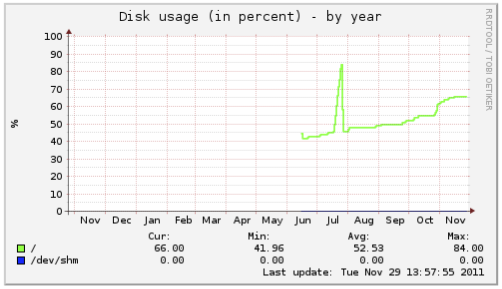
\includegraphics[width=\linewidth, keepaspectratio = true]{media/disk-usage-by-year.png}
\mycaption{figure}{\label{abb:disk-usage-by-year}Verhältnis von Speicheplatzverbrauch zur Speicherkapazität in Prozent in einer Zeitspanne von einen Jahr}
\end{center}

\subsection{Zugriffswachstum}
Für die Ist-Aufnahme konnten keine historischen Messdaten zur Verfügung gestellt werden.

\subsection{Skalierbarkeit Datenvolumen}
Während dem Betrieb ist ein Ausbau der Speicherkapazität (Skalierbarkeit) nicht möglich. Eine Vergrösserung der Speicherkapazität ist nur durch einen Wechsel auf ein anderes Hostingprodukt möglich. Dies erfordert eine Migration auf eine neue Server-Plattform. 

\subsection{Skalierbarkeit Datenzugriffe}
Keine Skalierbarung möglich. 

\subsection{Daten Durchsatz I/O}
Für die Ist-Aufnahme konnten keine Messdaten zur Verfügung gestellt werden.

\subsection{Daten Redundanz}

Die Daten-Redundanz wird durch das RAID-5 gewährleistet.

\subsection{Datenverfügbarkeit}
Stromausfälle und Netzwerkstörungen im Rechenzentrum des Hosting Providers führten zu Störungen und Ausfällen in der Webapplikation und in der Datenauslieferung. Die Störungen wurden jedoch nicht dokumentiert, weshalb keine statistische messbare Aussage über die erreichte Datenverfügbarkeit gemacht werden kann.

\subsection{Daten Sicherheit}
Die Daten sind durch physischen Fremdzugriff mittels Verschlüsselung geschützt. Für die Verschlüsselung wird das Device Mapper Module dm-crypt eingesetzt. dm-crypt verschlüsselt die Daten bereits auf Blockebene und ist somit für das Dateisystem tranRAID-5nt.

\subsection{Daten Integrität}
Zu jedem Bild wird eine Hash Prüfsumme gespeichert, die bei jedem Sicherung geprüft wird. Die Daten-Integrität ist somit sichergestellt.

\subsection{Sicherung}
Es wird täglich mittels dem Tool ccollect\footnote{\url{http://www.nico.schottelius.org/software/ccollect/}} ein R-Sync Sicherung der Daten erstellt. Das Sicherung wird ausser Hause gelagert.

\subsection{Wirtschaftlichkeit}
Die Kosten für die Speicherung der Daten inklusive Webinfrastruktur sind vergleichsweise zu alternativen Lösungen tief.

\subsection{Lokalität}

Die Web-Applikation inklusive dessen \gls{Primären-Daten} werden am selben Standort betrieben. Die Sicherungsdaten werden an einen seperaten Standort gelagert. Der Zugriff auf Sicherungs-Daten ist innerhalb 30 Minuten möglich.

\section{Analyse-Ergebnisse}

\subsection{System-Architektur}

\subsection{Datenwachstum und Speicherkapazität}
Die Messdaten aus dem  \refabb{abb:disk-usage-by-year} zeigen, dass das Datenvolumen seit  Juni 2011 bis Ende November 2011 mit Ausnahme einer unregelmässigen Spitze und einem grösseren Wachstumsschub Ende Oktober kontinuierlich zugenommen hat. Die etwas erhöhte Spitze lässt sich durch eine vorübergehende technische Änderung am System erklären und hat somit für die Auswertung keine Relevanz. Während der erwähnten Zeitspanne hat das Datenvolumen von 1,634 Terabyte auf 2,546 Terabyte zugenommen. Dies entspricht einer Datenzuwachsrate von 0,912 Terabyte bzw. 55,8\% in fünf Monate. Das Durchschnittliche Datenwachstum beträgt 0,182 Terabyte bzw. 11,1\% pro Monat.

Setzt sich der bisherige Trend fort, so ist die verfügbare Speicherkapazität von 3,8 Terabyte in weniger als 7 Monate erschöpft. Berücksichtigt man bei diesem durchschnittlichen Datenwachstum mögliche Wachstumsschübe für Neukunden, welche durch das Einlesen von deren bestehende Bilddatenbanken entstehen könnten, so reduziert sich die Kapazitätsreserve nach unten und würde eine vorzeitige Umstellung auf ein neues System bedingen.

Gemäss des Auftraggebers ist ferner ein neues Feature für die Web-Applikation geplant, welches den Speicherplatzbedarf verdoppeln würde. Die aktuelle Speichersituation lässt momentan den produktiven Einsatz des neuen Feature nicht zu. Das durchschnittliche Datenwachstum würde voraussichtlich auf 0,364 Terabyte pro Monat steigen.

Die jetzige Speicherkapazität erfüllt schon heute die Anforderungen nicht mehr.

\begin{equation}
\mbox{Datenwachstum}_{Monate5} = 2,546  \mathrm{TB} - 1,634 \mathrm{TB} =  0,912 \mathrm{TB}
\label{eqn:Verfügbarkeit_5Monate}
\end{equation}

\begin{equation}
\mbox{Datenwachstum}_{Monate5} = \frac{0,912 \mathrm{TB}}{\frac{1,634 \mathrm{TB}}{100 \%}} =  55,813\%
\label{eqn:Verfügbarkeit_5Monate_in_Prozent}
\end{equation}

\begin{equation}
\mbox{Durchschnittliches Datenwachstum}_{Monate} = \frac{0,912 \mathrm{TB}}{5\mathrm{m}} =  0,1824 \mathrm{TB}
\label{eqn:Verfügbarkeit_1Monate}
\end{equation}

\begin{equation}
\mbox{Durchschnittliches Datenwachstum}_{Monate} = \frac{55,813\%}{5 \mathrm{m}} = 11,162\%
\label{eqn:Verfügbarkeit_1Monate_in_Prozent}
\end{equation}

\subsection{Skalierbarkeit Datenvolumen}\label{AnalyseSkalierbarkeitDatenvolumen}
Die Eingesetzte Speicherarchitektur lässt eine Skalierung des Datenvolumen mittels hinzufügen von weiteren Festplatten oder durch Migration auf grösseren Festplatten zu. Die maximale Anzahl von Festplatten wird dabei durch die Anzahl vorhandenen SATA Anschlüsse im Server bestimmt. Beim eingesetzten Server handelt sich um eine Hosting Produkt welche meist begrenzt ausbaubar ist. Bei Hosting Produkte erfolgt eine Skalierung meist durch eine Wechsel auf eine besser ausgebautes Hosting Produkt. 

\subsection{Skalierbarkeit Datenzugriffe}
Eine mögliche Skalierung bezüglich des Datendurchsatzes könnte durch schnellere Festplatten, durch eine optimierte Verteilung der I/O-Operationen auf verschiedene Festplatten oder durch die Verteilung der Daten auf weitere Systeme erreicht werden. Zu beachten sind auch hier dieselben Prämissen, wonach wie beim Ausbau des Datenvolumens das bestehende System nur sehr begrenzt ausgebaut werden kann bzw. auf ein anderes Hostingprodukt migriert werden müsste.

\textbf{Skalierung durch schnellere Festplatten:}
Moderne Festplatten, mit Ausnahme von den teuren Solid State Disk (SSD), bieten zwar eine grössere Speicherdichte aber aufgrund der erreichten physikalischen Grenzen keine bedeutend effizientere IOPS versprechen. Eine Festplatte mit 7200 RPM erreicht durchschnittlich ein IOPS zwischen 75 und 100 IOPS. Bei SSD Disks wurden schon 1'190'000 IOPS in einem einzelnen PCI Geräte gemessen.\cite{Symantec2011} \cite{Fusionio} 
Ein Wechsel auf die genannten SSD Festplatten, ist aktuell noch mit sehr hohen Kosten pro Gigabyte verbunden. Gartner geht davon aus, dass 2012 die Preise pro Gigabyte bei SSD auf durchschnittliche 1\$ sinken werden. Gegenüber den heutigen Preisen bei konventionellen Festplatten von 30 Cents pro Gigabyte ist dies immerhin 3x teurer. Aus diesem Grund werden SSD Disks bei grossen Datenvolumen meist noch nicht eingesetzt, ausser spezielle Anforderungen an die Performance rechtfertigen die höhere Investition. \cite{AgamShah2011}

\textbf{Skalierung duch Verteilung der I/O Operationen:}
Ein RAID oder Volume Manager bietet die Möglichkeit, die I/O Operationen auf mehrere Festplatten zu verteilen. In einem RAID-5 verkleinert sich wie in Kapitel \refchap{AnalyseSkalierbarkeitDatenvolumen} beschrieben, die MTTF mit jeder weiteren Festplatte. Zudem sind die verfügbaren Anschlüsse in einem Server ebenfall ein zu berücksichtigen limitierender Faktor.

\textbf{Skalierung durch Verteilung der Daten:}
Nicht alle Kategorien von Daten haben die gleichen Anforderungen an den Durchsatz. Datenbanken z.B. benötigen in der Regeln einen höheren IOPS als statische Daten wie z.B. Bild-Daten, welche weniger oft abgefragt werden. Für die Verteilung der Daten ist eine Änderung in der System-Architektur und allenfalls in der Anwendungs-Architektur notwendig. Ein Beispiel für eine solche Anpassung der System-Architektur wäre die Auslagerung der Datenbank auf ein separates System, welches mit schnellen Solid State Disk ausgerüstet ist. 

\subsection{Redundanz}
Eine RAID-5 System bietet wie im \refsec{RAID-5} beschrieben, keine 1:1 Redundanz. Die Daten sind im RAID-5 nicht doppelt gespeichert, sondern werden bei einen Datenverlust mittels XOR Operation aus den Parität Stripes und den vorhandenen Daten Stripe-Einheiten berechnet. 

Bei einen Zugriff auf einen verlorenen Daten Stripe werden die Daten online berechnet. 

Treten bei einer Festplatte Fehler auf, werden die verlorenen Daten bei einem Zugriff aus dem Parität Stripe Einheit.??? Der Zugriff auf die Daten ist durch die Berechnung der Daten aus dem Parität Stripe Einheit Online möglich. Wird die ausgefallen Festplatte durch eine neu intakte Festplatte ersetzt, können die Daten durch einen Rebuild während des Betriebs wieder hergestellt werden. Durch die Berechnung und Schreib/Lese Operationen im RAID während des Wiederherstellungprozesses verschlechtert sich der Datendurchsatz und I/O Rate für den Datenzugriff wesentlich.

Einen Ausfall einer weiteren Festplatten kann das RAID-5 System nicht mehr kompensieren und führt zu einem physischen Datenverlust aller Online-Daten. Die Daten müssen in der Folge mittels des Sicherung eingelesen und wiederhergestellt werden, was jedoch nur im Offline-Betrieb möglich ist. 

Bei Festplatten welchen aus dem gleichen Produktionszyklus stammen, kann die Wahrscheinlichkeit eines weiteren Ausfall höher sein, im vergleich zu Festplatten die aus unterschiedlichen Produktionszyklen stammen.

\subsection{Service- und Daten-Verfügbarkeit}
Die bisherige System-Architektur gemäss dem Ist-Bestand ermöglichen keine AEC-2 Hochverfügbarkeit. Grund dafür ist die Fokussierung auf einen einzelnen Server in der System-Architektur. Der Server stellt eine "'Single Point of Failure"' (SPOF) dar. Tritt beim Server eine Störung auf, wie Sie zum Beispiel Aufgrund eines Gerätedefekts oder Softwarefehler auftreten können, kann der Service nicht von einem redundantem System übernommen oder weitergeführt werden. Eine Störung kann also die Verfügbarkeit während den Betriebszeiten starl gefährden und entspricht nicht den heutigen Anforderungen.

Die Netzwerkverfügbarkeit wird vom Hosting Anbieter gemäss den Allgemeinen Geschäftsbedingungen \cite{Ag2009} mit einer Verfügbarkeit von 99\% im Jahresmittel gewährleistet. Die Verfügbarkeit könnte somit bei einem 24x365 Stunden Betrieb während 87,6 Stunden nicht gewährleistet sein.

Das Speichersystem für sich selbst betrachtet kann die Verfügbarkeit und die Daten-Integrität gewährleisten, sofern keine Störungen durch einen Festplattendefekt eintreten. Das Speichersystem, welches ein interner Block-basierenden RAID-5 Speicher darstellt, ist ein Bestandteil des Serversystems und weist deshalb die selbe Verfügbarkeitsstufe wie das Serversystem auf. Die Service und Datenverfügbarkeit weist aus den genannten Gründen eine Verfügbarkeit Stufe von '"Highly Reliable"' AEC-2 auf.

Die im \refsec{System-Architektur}  beschriebene System-Architektur gewährleistet keine Hochverfügbarkeit der Daten. Einer der Gründe dafür ist, dass die Applikation nur auf einem einzelnen Server betrieben wird, dessen Hardware mit Ausnahme der Festplatten keine Redundanz aufweist und nicht für Hochverfügbar ausgelegt ist. 

Die Applikation wird auf einem einzelnen Server betrieben. Der Server und dessen Hardware mit Ausnahme der Festplatten stellen einen "'Single Point of Failure"' (SPOF) dar. Fällt der Server wegen eines Hardwaredefektes oder einem Softwarefehler aus, sind Daten und Anwendung für den Endbenutzer nicht mehr verfügbar.

Zudem werden die Daten und Applikation nur an einem Standort betrieben. Treten unvorhersehbare Ereignisse auf, wie z.B. ein lokaler Stromausfall, ein Brand oder eine Naturkatastrophe, kann der Betrieb nicht ohne die Wiederherstellung des ganzen Systems inklusive Daten von Sicherung wieder aufgenommen werden. Sofern nicht ein gemieteter Ersatzserver bereitsteht, muss ebenfalls die Beschaffung und Installation eines neuen Systems bei einem anderen Hosting Provider zur Ausfallzeit (Downtime) mit einberechnet werden. Der Service wäre während einer längeren Zeit nicht mehr verfügbar. Ein Kundenverlust und weitere Konsequenzen könnten die Folge sein.

\subsection{Daten Sicherheit}
Durch die Festplattenverschlüsselung sind die Daten bei abgeschaltetem Server vor unberechtigten Zugriffen geschützt. Befindet sich der Server jedoch im laufenden Betrieb, bietet die Verschlüsselung keinen Schutz vor Datendiebstahl. 

In einem Interview mit Ben Schwan im Technology Review hat Edward W. Felden, Professor für Informatik an der Princeton University den Grund dafür erklärt. 

\begin{quotation}\em
... ,die Dechiffrierungsschlüssel bei einer Festplattenverschlüsselung sitzen immer irgendwo im DRAM-Speicher. Um an sie heranzukommen, schaltet der Angreifer zunächst den Strom des Rechners aus und stellt die Energieversorgung dann gleich wieder her. Dann bootet er die Maschine in ein spezielles, böswilliges Betriebssystem hinein. Zu diesem Zeitpunkt enthält der Speicher noch immer die Originalinformationen, die verfügbar waren, als der Rechner noch nicht abgeschaltet wurde – die gewünschten Schlüssel natürlich auch. Das kurze Abschalten des Stroms hat daran rein gar nichts geändert. Der Angreifer kann dann die gewünschten Dechiffrierungsschlüssel aus dem Speicher auslesen und damit die geschützten Informationen auf der Festplatte jederzeit entschlüsseln\end{quotation}\cite{Schwan2008}

Des weiteren bietet eine Festplatten keinen Schutz bei Schwachstellen in der Software oder  der Konfiguration im laufenden Betrieb. Grund dafür ist, dass das Betriebsystem und Anwendungen über eine Verschlüsselungsschicht unverschlüsselt zugreifbar sind.


%!TEX root=../documentation-bachlorthesis-speicherarchitektur-lstucker.tex

\cleardoublepage
\chapter{Szenarien Beschreibung}
Der Auftraggeber hat gewünscht, bei der Evaluation der Speicherlösungen mehrere Szenarien in der Volumenentwicklung über die Zeit zu berücksichtigen. 

Die beschriebenen Szenarien sind mit den Auftraggeber besprochen worden. Die folgenden Annahmen wurden nicht aufgrund eines vorhandenen Geschäftsplan aufgebaut und können von den definierten Geschäftszielen des Auftraggebers abweichen. 


\section{Szenario-1 Schwaches Datenvolumen und geringes Wachstum im Datenzugriff}\label{Szenario1}
Bei Szenario-1 wird angenommen, dass sich der Kundenzuwachs, welche die Dienstleistung zur Speicherung und Aufbereitung Ihrer Bilddaten verwenden, marginal steigert. In diesen Fall beträgt das durchschnittliche Datenwachstum 0.25 Tebibyte pro Monat und bewegt sich in einem vergleichbaren Umfang wie im bisherigen Umfang, siehe Beschrieb des Ist-Zustands.


Datenwachstum in Tebibyte pro Monat: 0.25 Tebibyte

Bilder\footnote{Durchschnittsgrösse von 100 Mebibyte pro Bild} Zuwachs pro Monat: 4'690 Bilder

Speichervolumen in 36 Monaten: 11.5 Tebibyte

Anzahl Bilder\footnotemark[\value{footnote}] in 36 Monaten: 168'821 Bilder

\section{Szenario-2 Starkes Wachstum der Daten / starkes Wachstum der Abfragen}
Im Szenario-2 wird davon ausgegangen, dass die Kundenbasis im Vergleich zum Ist-Zustand stark anwächst. Durch die substantielle Zunahme an Neukunden beträgt der durchschnittliche Datenzuwachs 6 Tebibyte pro Monat.


Datenwachstum in Tebibyte pro Monat: 6 Tebibyte

Bilder\footnotemark[\value{footnote}] Zuwachs pro Monat: 12'583 Bilder

Speichervolumen in 36 Monaten: 218,5 Tebibyte

Anzahl Bilder\footnotemark[\value{footnote}] in 36 Monaten: 458'228 Bilder
 

%!TEX root=../documentation-bachlorthesis-speicherarchitektur-lstucker.tex
\cleardoublepage
\chapter{Soll-Analyse}
Bei der Soll-Analyse sollen die erarbeiteten Szenarien aus dem Szenarienbeschrieb berücksichtigt werden. 

\section{Szenario-1}\label{Soll-1}

\subsection{Verfügbarkeit}
Die Verfügbarkeit soll durchgehend von Speichersystem bis zum Web-Service mindestens dem AEC-2 Standard von Harvard Research entsprechen. Dies bedeutet, dass die Verfügbarkeit der Applikation, beziehungsweise der Daten, dass der Betrieb nur innerhalb festgelegter Zeitblöcke, beziehungsweise nur während der Hauptbetriebszeit minimal unterbrochen werden darf. Die bestehende Infrastruktur besteht nur aus einem einzelnen Web-Server. Dieser enthält gleichzeitig auch das Speichersystem mit seinen internen Festplatten, welche mit einem RAID-5 zusammengefasst sind. Eine defekte Komponente des Web-Servers würde das gesamte System zum Erliegen bringen. Wie in der Ist-Analyse beschrieben, erfüllt das Speichersystem für sich alleine zwar eine genügende Verfügbarkeit gemäss Definition von Harvard Research von AEC-2. Die restlichen Komponenten bzw. Softwarekomponenten des Web-Services, erfüllen diesen Anspruch allerdings nicht. Die bestehende Speicherarchitekur kann den Speicher nicht ohne Anpassung der Architektur, an weitere Web-Server zur Verfügung stellen.

Die Daten müssen mindesten in einfacher Redundanz vorhanden sein. 

Um den AEC-2 Standard zu erfüllen, ist es nicht notwendig, dass die \gls{Primearen-Daten} standortübergreifend verfügbar sind.

\subsection{Datenzugriff}
Die bestehende Speicherarchitektur konnte die bisherigen Datenzugriffe mit einem Web-Server zufriedenstellend erfüllen. Es wird davon ausgegangen, dass sich die Anzahl Datenzugriffe für die Bildaufbereitung und Speicherung von neuen Bilddaten nicht weiter steigert. Mit der erhöhten Anforderung bezüglich der Verfügbarkeit ist es notwendig, dass der Datenzugriff auf das Speichersystem von mindestens einem weiteren Web-Server erfolgen kann. 

Der \gls{POSIXIO} Zugriff soll nach Möglichkeit für die einfache Integration in die Web-Applikation unterstützt werden.

Der simultane Lesezugriff auf das gleiche Objekt muss unterstützt werden.

Der simultane Schreibvorgang auf ein Objekt muss nicht unterstützt werden.

\subsection{Speicherkapazität}
Für die Erfüllung der Speicheranforderungen des Szenario-1 muss das Speichersystem den Speicherausbau auf mindestens 16.1 Tebibyte unterstützen. In den 16.1 Tebibyte ist eine Reserve von 40\% für ein mögliches künftiges Wachstum oder als Migrationsreserve einkalkuliert. Nicht berücksichtigt ist eine gewollte Redundanz der Speicherkapazität.

Das Speichersystem soll ca. 400'000 Objekte verwalten können.

Das Speichersystem soll zudem die Speicherung von Objekten von bis zu 2 Gibibyte Grösse unterstützen.

\subsection{Datenqualität}

Die Selbstheilung von Objekten ist nicht gefordert kann aber als Option berücksichtigt werden.

Die standortübergreifende Datensicherung soll möglich sein.
Die konsistente Wiederherstellung der Daten aus einer Sicherung muss möglich sein. 

\subsection{Vergleich mit Ist-Zustand}
Im Vergleich der neuen Anforderungen mit dem Ist-Zustand ergeben sich folgende Vorteile:

\begin{itemize}
\item Durchgehende Verfügbarkeit nach AEC-2 Standard
\item Redundante Web-Server
\item Kein Single Point of Failure
\item Erfüllt die Anforderungen an die Speicherkapazität für die nächsten 3 Jahre
\item Ermöglicht mehrere gleichzeitige Lesezugriffe auf das gleiche Objekt
\end{itemize}

\section{Szenario-2}

\subsection{Verfügbarkeit}
Die Verfügbarkeit soll dem AEC-4 Standard von Harvard Research entsprechen. Das bedeutet, dass die Applikationen und Daten unterbrechungsfrei verfügbar sein müssen.  Der 24*7 Betrieb (24 Stunden, 7 Tage die Woche) muss gewährleistet sein. Bei hoher Kundenzahl und Speichervolumen würde ein Betriebsunterbruch der Web-Services grossen Imageschaden verursachen und die Kunden bezüglich der Zuverlässigkeit der benötigten Services verunsichern.

Die Daten müssen mindesten in einfacher, idealerweise in doppelter Redundanz vorhanden sein. 

Die \gls{Primearen-Daten} müssen mindestens an zwei Standorten gehalten werden.

\subsection{Datenzugriff}
Durch die gleichzeitig vielen Datenzugriffe muss es möglich sein, die Daten durch mehrere Web-Server zur Verfügung zu stellen.

Der \gls{POSIXIO} Zugriff soll nach Möglichkeit für die einfache Integration in die Web-Applikation unterstützt werden.

Der simultane Lesezugriff auf das gleiche Objekt muss möglich sein.

Der simultane Schreibvorgang auf ein Objekt muss nicht unterstützt werden.

\subsection{Speicherkapazität}
Für die Erfüllung der Speicheranforderungen des Szenario-2, muss das Speichersystem 306 Tebibyte unterstützen. In den 306 Tebibyte ist eine Reserve von 40\% für ein mögliches künftiges Wachstum oder als Migrationsreserve einkalkuliert. Nicht berücksichtigt ist eine gewollte Redundanz der Speicherkapazität.

Geht man von einem Datenzuwachs von 6 Tebibyte pro Monat aus, wird das Speichervolumen für alle Bilddaten nach 36 Monaten bereits 218,5 Tebibyte betragen. Berücksichtigt man zusätzliche Reserven von 40\%, so muss das Speichersystem mindestens 306 Tebibyte zur Verfügung stellen. Darin ist die Datenredundanz nicht eingerechnet.

Das Speichersystem soll 9'500'000 Objekte verwalten können.

Das Speichersystem soll zudem die Speicherung von Objekten von bis zu 2 Gibibyte Grösse unterstützen.

\subsection{Datenqualität}
Wegen der grossen Datenmenge soll die Selbstheilung von Objekten unterstützt werden. Damit verringert sich der Bedarf für die manuelle Wiederherstellung eines Objektes.

Die standortübergreifende Datensicherung soll möglich sein.
Die konsistente Wiederherstellung der Daten aus einer Sicherung muss möglich sein.

\subsection{Vergleich mit Ist-Zustand}
Im Vergleich der neuen Anforderungen mit dem Ist-Zustand ergeben sich folgende Vorteile:

\begin{itemize}
\item Durchgehende Verfügbarkeit nach AEC-7 Standard
\item Redundante Web-Server
\item Kein Single Point of Failure
\item Erfüllt die Anforderungen an die Speicherkapazität für die nächsten 3 Jahre
\item Unterstützung von Selbstheilung von korrupten Objekten
\item Ermöglicht mehrere gleichzeitige Lesezugriffe auf das gleiche Objekt
\end{itemize}
%!TEX root=../documentation-bachlorthesis-speicherarchitektur-lstucker.tex

\cleardoublepage
\chapter{Entscheidungsfindung bei Evaluationen}\label{kab:Entscheidungsfindung}
\section{Grundlagen}
Evaluation ist der systematische Prozess der Datensammunlung und Analyse, um eine Entscheidung treffen zu können.
\section{AHP}
Für das Evaluations- bzw. Bewertungsverfahren wurde das Analytische Hierachie-Prozess-Verfahren (AHP) angewendet. AHP wurde in den siebziger Jahren von Thomas L. Saaty zur Lösung mehrkriterieller Entscheidungsprobleme entwickelt und basiert unter anderem auf einem mathematischen Modell.
\cite{Reichardt2003}

Der Entscheidungsprozesse ist beim AHP wie der Name ausdrückt eben analytisch und hierarchisch. Die Analyse beruht auf mathematischen und logischen Entschlüssen. Auf das genaue mathematische Verfahren wird in dieser Arbeit nicht eingegangen. Sie kann in diverser Literatur nachgelesen werden. \cite{Reichardt2003}

Im AHP Verfahren werden alle Kriterien derselben Ebene in Paarvergleiche bewertet und anhand 9-Punkte-Bewertungsskale aus der \reftab{tab:9PBewertungsskala} bzw. der umgekehrten Relation aus der \reftab{tab:UmgekehrteBewertungsskala} gewichtet.

Nach der Berechnung der Kriterien-Prioritätenbestimmung, werden die Alternativen in Paarvergleiche zu jedem Kriterium anhand derselben 9-Punkte-Bewertungsskale verglichen und bewertet. Anschliessend wird wiederum durch Berechnung der Gewinner ermittelt.

\begin{table}[htbp]
\caption{9-Punkte-Bewertungsskala \cite{Reichardt2003}}
\begin{tabular}{|c|L{3.5cm}|L{8.5cm}|}
\hline
\multicolumn{1}{|l|}{} & Definition & Interpretation \\ \hline
 1 &  gleiche Bedeutung &  Beide verglichenen Elemente haben die gleiche ""Bedeutung für das nächsthöhere Element. \\ \hline
3 &  etwas grössere "" ""Bedeutung & 
Erfahrung und Einschätzung sprechen für eine ""
etwas größere Bedeutung eines Elements im 
Vergleich zu einem anderen \\ \hline
5 &  erheblich grössere "" Bedeutung & 
Erfahrung und Einschätzung sprechen für eine "" 
erheblich größere Bedeutung eines Elements im ""
Vergleich zu einem anderen \\ \hline
7 &  sehr viel grössere ""Bedeutung & 
Die sehr viel größere Bedeutung eines Elements 
hat sich in der Vergangenheit klar gezeigt. \\ \hline
9 &  absolut dominierend &  Es handelt sich um den größtmöglichen ""
Bedeutungsunterschied zwischen zwei 
Elementen \\ \hline
\multicolumn{1}{|l|}{2,4,6,8} & Zwischenwerte &  \\ \hline
\end{tabular}
\label{tab:9PBewertungsskala}
\end{table}

\begin{table}[htbp]
\caption{Umgekehrte Relationen der Bewertungsskala \cite{Reichardt2003}}
\begin{tabular}{|c|L{3.5cm}|L{7.3cm}|}
\hline
\multicolumn{1}{|l|}{} & Definition & Interpretation \\ \hline
1 & gleiche Bedeutung & Beide verglichenen Elemente haben die gleiche 
Bedeutung für das nächsthöhere Element. \\ \hline
 1/3 & etwas geringere Bedeutung & Erfahrung und Einschätzung sprechen für eine 
etwas geringere Bedeutung eines Elements im 
Vergleich zu einem anderen.  \\ \hline
 1/5 & erheblich geringere Bedeutung & 
Erfahrung und Einschätzung sprechen für eine 
erheblich geringere Bedeutung eines Elements im 
Vergleich zu einem anderen \\ \hline
 1/7 & sehr viel geringere Bedeutung & 
Die sehr viel geringere Bedeutung eines Elements 
hat sich in der Vergangenheit klar gezeigt \\ \hline
 1/9 & absolut unterlegen & Es handelt sich um den größtmöglichen 
Bedeutungsunterschied zwischen zwei 
Elementen \\ \hline
\multicolumn{1}{|l|}{1/2, 1/4, 1/6, 1/8} & Zwischenwerte &  \\ \hline
\end{tabular}
\label{tab:UmgekehrteBewertungsskala}
\end{table}

\subsection{Software Unterstützung}
Der Berechnungsaufwand nimmt mit zunehmender Anzahl Alternativen und Kriterien zu. Aus diesem Grund ist es empfehlenswert, die Evaluation Software-unterstützt durchzuführen.

Alle Berechnungen in dieser Arbeit wurden mit der Software "'AHP Decision"' von "'True North Software"' durchgeführt.

%!TEX root=../documentation-bachlorthesis-speicherarchitektur-lstucker.tex
\cleardoublepage
\chapter{Speicherarchitekturen}

Sowohl private Personen als auch Unternehmen haben unterschiedliche Anforderungen an die Speicherung ihrer Daten. Während früher die Daten in der Regel in einem integrierten Speicher des Computersystems verwaltet wurden, werden heute eine breite Paletten an Speicherlösungen am Markt angeboten. Ein Grund dafür ist der kontinuierlich wachsende Bedarf an mehr Speicherkapazität aber auch zusätzliche Anforderungen an die Verwaltung der Daten, die Datensicherung. Spezifische Daten zu suchen und zu bearbeiten soll heute einfach, effizient und zu günstigen Kosten möglich sein, was laufend neue Lösungsansätze bedingt und es nicht einfacher macht, auf das richtige Pferd bzw. Technologie zu setzen. Wer möchte morgen schon gezwungen sein, seine mühsam aufbereiteten Daten in einem aufwendigen Migrationsverfahren, womöglich mit einem notwendigen Datenverlust, in ein neues System zu übernehmen? Eine genauere Betrachtung des Angebotsmarktes für die vorhandenen und die künftigen sich durchzusetzenden Technologien drängt sich deshalb auf.

Die heutigen am Markt erhältlichen Speicherarchitekturen lassen sich in der obersten Kategorie in Block- (Block-based), Datei- (File-based) und Objekt- (Object-based) basierte adressierende Systeme unterteilen. Die Kategorien zur Einteilung der verschiedenen Lösungen lässt sich nicht exakt zuordnen, da einige Speicherlösungen aus einem Mix aus mehreren Kategorien bestehenden können.

\section{Block-basierend}
Die Block-basierende Speicherarchitektur ist wohl die traditionellste von allen und ist die am weitverbreiteste Form. Die meisten Computersysteme, sei es Server, Desktop-PCs, Tablet-PC, Smartphones, Spielkonsole, verwaltet ihre Daten in einem blockbasierenden Speicher. Als Speichermedium wird in diesen Geräten oft eine magnetische Festplatte, Solid State Disk oder ein Flash-Speicher verwendet.

Bei Block-Speicher werden Daten in Blöcke gelesen und gespeichert (adressiert), ein Block bildet sich aus einer Sequenz von Bits bzw. Bytes. Die Grösse eines Blocks wird als Blocklänge bezeichnet und ist bei allen Blöcken einer Einheit gleich gross. 

Experten wie Mike Mesnier, Greg Ganger und Erik Riedel, sehen jedoch bei zunehmender Speichergrösse und Komplexität von Systemen fundamentale Einschränkungen von Block-Schnittstellen.

\begin{quotation}
\em Since the first disk drive in 1956, disks have grown by over six orders of magnitude in density and over four orders in performance, yet the storage interface (i.e., blocks) has remained largely unchanged. Although the stability of the block-based interfaces of SCSI and ATA/IDE has benefited systems, it is now becoming a limiting factor for many storage architectures. As storage infrastructures increase in both, size and complexity, the functions that system designers want to perform are fundamentally limited by the block interface. \end{quotation}\cite{Mesnier2003}

Vergleicht man die Performance der ersten Festplatte, welche von IBM produziert wurde, mit einer heute erhältlichen Seagate Festplatte (Jahr 2011), so hat sich die Speicherdichte von 2000 bit per Quadratzoll auf 625 Gigabyte und die Transferrate von 8 Kilobyte auf 600 Megabyte pro Sekunde verbessert. \cite{Seagate2011}\cite{Seagate2011a}

Für den Zugriff auf blockbasierende Speichersysteme werden meist Schnittstellen-Protokolle wie das Small Computer System Interface (SCSI) oder Advanced Technology Attachment (\gls{ATA}) verwendet. Diese Protokolle wurden jedoch in einer Zeit entwickelt, als man davon ausging, dass ein Blockspeicher jeweils nur von einem Computersystem verwendet wird und nicht mit mehreren Computersystemen geteilt werden soll. Diese Annahme für single user systems stimmt für den Consumer Elektronic Bereich mehrheitlich noch heute. In Bereichen jedoch, in denen grosse Speicherkapazitäten oder eine hohe Verfügbarkeit für viele gleichzeitige Benutzer gefordert sind, wie dies viele Geschäftsanwendungen charakterisiert, stimmen diese Annahmen nicht mehr.

Für blockbasierende Speicher, welche nicht als Server-interne Speicher bestehen, unterscheidet man den Direct Attached Storage (DAS) und das Storage Area Network (SAN). 

\subsection{Direct Attached Storage}
Bei DAS handelt es sich, wie es aus der englischen Bezeichnung zu entnehmen ist, um Speicher, welcher direkt an ein Computersystem angeschlossen wird. Bei DAS Enclosure handelt sich um ein Gehäuse mit mehreren verbauten Festplatten, welche üblicherweise über einen Host-Bus-Adapter an ein Computersytem angeschlossen werden. Als Schnittstellen-Protokoll werden \gls{ATA}, \gls{SATA}, \gls{eSATA}, \gls{SCSI}, \gls{SAS} oder Fibre Channel eingesetzt. DAS können mit mehreren Computersystemen geteilt werden, sofern genügend Schnittstellen zur Verfügung stehen.

\subsection{Storage Area Network}
Die Storage Networking Industry Association (\gls{SNIA}) definiert ein Storage Area Network (SAN) als ein Netzwerk, dessen primärer Bestimmungszweck das Transferieren von Daten zwischen Computersysteme und Speicherelemente und unter Storage Elemente ist. Ein SAN besteht aus einer Kommunikations-Infrastruktur, welches eine physische Verbindung und eine Management-Schicht beinhaltet, das die Verbindungen, die Speichereinheiten und das Computersystem organisiert, damit der Datentransfer sicher und robust erfolgen kann. Der Begriff SAN wird normalerweise (aber nicht notwendigerweise) mit dem Block I/O Service in Verbindung gebracht und weniger mit dem Datei-Zugriff-Service. \cite{SNIA2011}

Je nach SAN Implementierung kommen folgende Geräte bzw. Komponenten vor:
\begin{itemize}
\item Server
\item Host Bus Adapter
\item Gigabit Interface Converter
\item SAN-Switch
\item Storage system (Speichersystem)
\item Tape Library
\item Logical Unit
\end{itemize}

\paragraph*{Server} 
Der Server greift über das SAN auf Ressourcen von Speichersystem oder Tape Library zu. In einzelnen Fällen kann der Server selbst über SAN anderen Servern Speicher zur Verfügung stellen.

\paragraph*{Host Bus Adapter}
Host Bus Adapter (HBA) für das SAN sind intelligente Hardwareschnittstellen, welche für die Verbindung von Server in einem SAN verwendet werden. Sofern die Server nicht bereits mit einem Host Bus Adapter ausgerüstet sind, können diese normalerweise durch Host Bus Adapter in form von Steckkarten erweitert werden. Der Host Bus Adapter selber hat pro Port einen Einschub, in welche ein Gigabit Interface Converter eingebaut wird. \cite{Christopher2009}

\paragraph*{Gigabit Interface Converter}
Der Gigabit Interface Converter ist eine modulare Schnittstelle, welche elektrische Signale in optische Signale umwandeln. \cite{SNIA2011}

\paragraph*{SAN-Switch}
Der SAN Switch ist ein Koppler, welcher dezidiert für die SAN-Umgebung verwendet wird.

\paragraph*{Speichersystem}
Das Speichersystem stellt im SAN den geteilten Speicher zur Verfügung. Gemäss den IT Marktforschung und Analyse Unternehmen Gartner gehören \gls{EMC}, \gls{IBM}, NetApp, \gls{Dell}, \gls{HP}, \gls{HitachiDataSystems} zu den Marktführern. \cite{RogerW.CoxPushanRinnenStanleyZaffos2011}

\paragraph*{Tape Library}
Tape Library ist eine Bandbibliothek, in welchem sich ein oder mehrere Bandlaufwerke und mehrere Magnetbänder befinden und meistens der automatische Bandwechsel mittels eines Bandroboters realisiert wird. Das Tape Library wird für die Sicherung von Daten auf Band eingesetzt.

\paragraph*{Logical Unit}
Ein Logical Unit ist ein Gerät, welches über SCSI-Protokoll über das Logical Unit Number (LUN) andressiert wird. Das Gerät wird, technisch nicht korrekt, oft als LUN bezeichnet. Im Speichersystem werden z.B. mehrere Festplatten mittels RAID zu einer Einheit zusammengefasst. Sofern keine weitere Virtualisierung von dem Speicherhersteller zum Einsatz kommt, wird die zusammengefasste Einheit wiederum in Speichereinheiten aufgeteilt und diese als LUN dem Server zugeteilt. \cite{SNIA2011}

\subsubsection{Fibre Channel}
SCSI ist zwar sehr populär, ist jedoch mit 80 Mbps Geschwindigkeit, mit maximal 25 Meter Buslänge und mit maximal 32 Geräten pro Bus, ein limitierender Faktor für viele Anwendungen. Unter anderem wegen den erwähnten Limitierungen von SCSI hat das American National Standards Institute (ANSI) die Fibre Channel Technik entwickelt. Fibre Channel ist ein mehrschichtiges Netzwerk, welches die charakteristischen Funktionen für die Übertragung von Daten über ein Netzwerk definiert. Der Standard enthält von der physikalischen Schnittstelle, Daten Codierung, Übertragungssteuerung (Link Control), Fluss Kontrolle, bis hinzu den Protokoll Schnittstellen. Im Vergleich zu anderen Netzwerken beinhaltet die Fibre Channel Architektur einen signifikanten Anteil von Hardware Prozessen, um eine hohe Performance zu erreichen. \cite{Gupta2002}\cite{Christopher2009}

Beim Design von Fibre Channel hat man darauf geachtet, die besten charakteristischen Eigenschaften der I/O Bus-Kommunikation (Channel) zwischen zwei Geräten und der Netzwerk- Kommunikation zwischen mehreren Geräten zu kombinieren. Die Channel-Kommunikation ist im Vergleich zur Netzwerk-Kommunikation, hardwareintensive, schnell und produziert wenig Overhead. Netzwerk-Kommunikation ist hingegen abhängig von der Softwareimplementierung, das Protokoll, unterstützt aber die Kommunikation für eine grosse Anzahl von Geräten.

Anders als es der Namen von Fibre-Channel vermuten lässt, ist Fibre-Channel nicht auf Fiberoptik-Kabel als Träger-Medium beschränkt, sondern lässt sich ebenso mit Kupferkabel betreiben. Aufgrund von physikalischen Eigenschaften ist das Fiberoptik-Kabel gegenüber dem Kupferkabel in Geschwindigkeit kombiniert mit Distanz überlegen. So liegt die maximale Distanz bei Kupferkabel bei 30 Metern bei einer Geschwindigkeit von 1 Gbps, bei höheren Geschwindigkeiten wird die maximale Distanz noch weiter reduziert. Beim Fiberoptic-Kabel wird die maximale Distanz der Signalübertragung von der Installationsqualität, des Fiberoptic-Kabeltyps, des Kern-Durchmessers, der Lichtwellenlänge Rundreise Latenz und der eingesetzter Hardware bestimmt. Je weiter das Licht innerhalb des Kabels übertragen werden muss, desto grösser ist der Verlust der ursprünglichen Signalstärke. Mit spezieller Hardware können auch Distanzen von bis zu 600 Kilometer \footnote{\url{http://www.enterprisestorageforum.com/industrynews/article.php/2171801/Synchronous-SAN-Sets-Fibre-Channel-Distance-Record.htm}} erreicht werden.

Es gibt drei Fibre Channel Topologien:
\begin{itemize}
\item Point-to-Point
\item Arbitrated-Loop
\item Switched-Fabric
\end{itemize}

\paragraph*{Point-to-Point-Topologie}
Die Point-to-Point-Topologie ist die direkte Verbindung von zwei Fibre Channel Geräten. Oft handelt es sich um eine Verbindung von einem Server und einem Speichersystem, wie dies im Direct Attached Storage (DAS) Umfeld vorkommt. \cite{Christopher2009}

\paragraph*{Arbitrated-Loop-Topologie}
Bei der Arbitrated-Loop-Topologie können bis zu 126 Knoten (NL\_Ports) in einem geteilten Bus-Ring zusammengeschlossen werden. In diesem Ring kann eine Verbindung zwischen zwei Ports aktiv sein, während alle anderen Ports als Repeater arbeiten und das Signal weiterleiten. Die Arbitrated-Loop-Topologie ist in seiner Architektur dem Token-Ring ähnlich. \cite{Gupta2002}\cite{Christopher2009}

\paragraph*{Switched-Fabric-Topologie}
Die klassische SAN Topologie basiert auf der Switched-Fabric-Topologie. Eine Switched-Fabric-Topologie besteht aus einer oder mehreren Switches, die zu einer Fibre-Channel-Fabric zusammengeschlossen werden. Die einzelnen involvierten FC-Geräte, wie Server oder Storagesysteme, werden über eine oder mehrere Ports an eine Switched-Fabric angeschlossen. In einer Fabric können bis zu $2^{24}$ Ports angeschlossen werden. \cite{Gupta2002}\cite{Christopher2009}

Mit der Switched-Fabic-Topologie lassen sich verschiedene Fabric Topologien bilden.
Die einfachste Topologie, welche die Eliminierung von "'Single Point of Failure"' zum Ziele hat, ist die Dual Switch Topologie, wie in der \refabb{abb:DualSwitchTopologie} dargestellt. In dieser Topologie dient jeder Switch als eigenständige Fabric. Die FC-Geräte wie Server und Storagesysteme werden jeweils pro Fabric bzw. Switch mit mindestens einem FC-Port angeschlossen. Durch den Einsatz von Path Management Software auf dem Server, kann eine vom Speichersystem zugeteilte Logical Unit über mehrere Path angesprochen werden. Diese Implementierung bietet gleich verschiedene Vorteile. Wenn ein Path oder eine ganze Fabric ausfallen sollte, übernimmt der andere Path automatisch die Kommunikation. Bei Wartungsarbeiten an Komponenten einer Fabric kann der Service ohne Downtime des Gesamtsystems weiter betrieben werden. Moderne Path Management Software und Speichersysteme unterstützen zudem die Lastverteilung (Loadbalance) der I/O-Last über alle Paths. \cite{Christopher2009}

\begin{center}
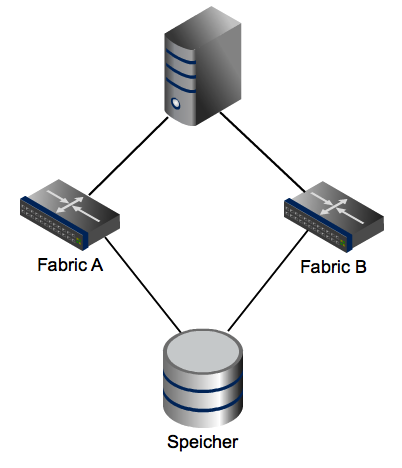
\includegraphics[width=\linewidth, keepaspectratio = true]{media/dualSwitchTopologie.png}
\mycaption{figure}{\label{abb:DualSwitchTopologie}Fibre Channel SAN mit Dual Switch Topologie}
\end{center}

Die Meshed Fabric Topologie erhöht die zusätzlich die Ausfallsicherheit innerhalb einer einzelnen Fabric. Für die Meshed Fabric sind pro Fabric mindestens vier Fibre Channel SAN Switches erforderlich. Jeder Switch wird, wie in \refabb{abb:MashedFabricTopologie} ersichtlich, mit mindestens einem Path, den sogenannten Inter-Switch-Link (ISL), zu allen anderen Switches in der Fabric verbunden. Die Meshed Fabric kann den gleichzeitigen Ausfall von mehreren Kabeln und Switches verkraften, ohne dass deshalb die ganze Fabric ausfällt. \cite{Christopher2009}

\begin{center}
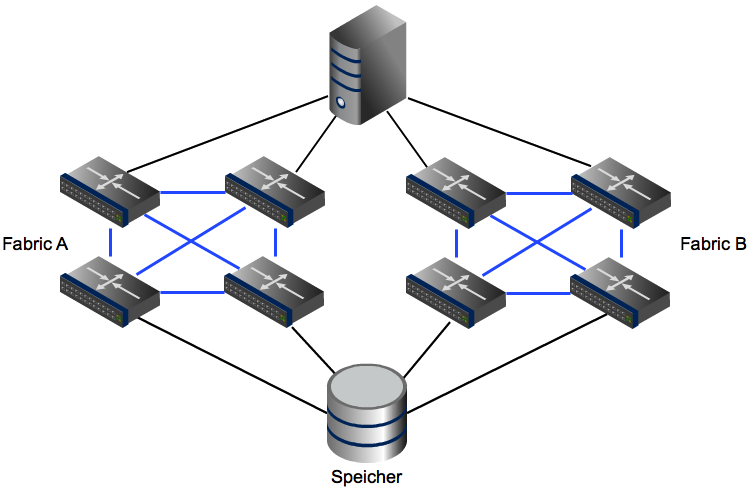
\includegraphics[width=\linewidth, keepaspectratio = true]{media/MashedFabric.png}
\mycaption{figure}{\label{abb:MashedFabricTopologie}Fibre Channel SAN mit Mashed Fabric Topologie}
\end{center}

\subsubsection{iSCSI}
Das SCSI-Protokoll ist ein populäres Protokoll für die Kommunikation mit I/O Geräten speziell für Speichergeräte. SCSI weist die Client-Server Architektur auf, wobei die Clients bei SCSI Interfaces als "initiators" bezeichnet werden und die logische Einheit vom Server als "target".

SCSI Protokoll wurde schon über Protokolle transportiert, jedoch waren all die Transportprotokolle in der Distanz limitiert. \gls{IBM} startete 1996 mit der Forschung für die Übertragung von SCSI über das Ethernet, dabei untersuchte \gls{IBM}, ob sich der Transport mittels IP oder \gls{TCPIP} besser eignen würde. Messungen zeigten damals, dass in einem lokalen Netzwerk der Transport mittels IP besser als \gls{TCPIP} geeignet ist. Mit den erwarteten künftigen Entwicklungen bezüglich des Datentransports über die lokalen Netzwerkgrenzen hinaus war hingegen der Einsatz von TCP/IP die bessere Wahl. 1999 hatten sich \gls{IBM} und \gls{Cisco} darauf geeinigt, "SCSI over TCP/IP" gemeinsam in einer Internet Engineering Task Force (\gls{IETF}) als Industriestandard weiterzuentwickeln \cite{JohnL.202}. Die definitive Spezifikation von SCSI over \gls{TCPIP} ist im \gls{RFC} 3720 mit dem Namen iSCSI im April 2004 fertiggestellt worden. \cite{J.Satran2004}

% \paragraph*{Kosten}
Für den Betrieb eines Fibre Channel SAN sind spezielle Hardware und Fibre Channel Kenntnisse notwenig. Da bei iSCSI dieselbe Technik wie im Computernetzwerk verwendet wird, benötigt der Aufbau und Betrieb von Netzwerk Infrastruktur und Management Software Lösungen keine zusätzliche Ausbildung, was die Gesamtbetriebskosten (TCO) substanziell senkt.

Grundsätzlich kann jeder Computer, welcher mit einem Netzwerkanschluss ausgerüstet ist und einen iSCSI Software Treiber hat, iSCSI nutzen. Computer, welche genügende Prozessorleistung aufweisen, können die zusätzliche Last für die Verarbeitung von iSCSI mit konventionellen Netzwerkkarten lösen. Computersysteme für welche die Verarbeitungsgeschwindigkeit kritisch ist, kann diese zusätzliche Last eine Bürde sein. Vergleichbar wie bei Fibre Channel gibt es für iSCSI spezielle Netzwerkkarten bzw. Host Bus Adapter, welche mittels TCP/IP Offload Engine (TOE) und volle iSCSI Offload Engine im eigenen Chip die \gls{TCPIP} bzw. iSCSI Pakete verarbeiten. Solche Netzwerkkarten entlasten die Central Processing Unit (\gls{CPU}) des Servers wesentlich und weisen bessere Werte in der Latenz auf.

% \paragraph*{Netzwerk}
In einem Ethernet Netzwerk verwaltet sich jeder Switch mehr oder weniger autonom und führt eine eigene Weiterleitungstabelle, mit welcher der Switch entscheidet, über welchen Port ein Ethernet Paket ausgeliefert werden muss. Dazu enthält die Weiterleitungstabelle pro MAC Adresse den dazugehörigen Port. Trifft ein Ethernet Paket mit noch unbekannter MAC Adresse ein, leitet der Switch das Paket über alle Ports weiter. Durch die Rückantwort vom Zielsystem lernt der Switch, über welchen Port dieses erreichbar ist. Werden in einem Switch Netzwerk benachbarte Switches untereinander über mehrere Pfade verbunden, kann es in einem solchen Szenario vorkommen, dass das Paket wieder am ursprünglichen Switch ankommt, wenn der benachbarte Switch die MAC-Adresse ebenfalls nicht kennt. Es entsteht dadurch eine Verdoppelung des Ethernet Paketes im Netzwerk bzw. es kommt zu einer Schleifenbildung, was in der Folge zu einer Netzwerkstörung führt. Mittels Spanning Tree Protokoll (STP) sollen solche Schleifen vermieden werden. Das Spanning Tree Protokoll erstellt eine Baum Topologie mit jeweils einem aktiven Path zwischen zwei Switches. Diese Topologie hat verschiedene Nachteile: 

\begin{itemize}
\item Beim Topologie-Wechsel wird im Netzwerk der Spanning Tree neu ausgehandelt. Während dieser Neuaushandlung ist der Datentransport während mindestens 15 Sekunden unterbrochen. Ein typischer Topologiewechsel kann zum Beispiel durch einen Pfad-Ausfall zwischen zwei Switches hervorgerufen werden.

\item In einer Baum-Hierarchie müssen die Pakete innerhalb des Baumes der Hierarchie entsprechend weitergeleitet werden (auf und ab) und können nicht über einen theoretisch direkteren Pfad quer weitergeleitet werden. Befindet sich z.B das Ziel auf der anderen Baumseite, muss das Paket die ganze Hierarchie hinauf und auf der anderen Seite hinunter bis zum Zielsystem weitergeleitet werden. Könnten die Switches über mehrere Pfade miteinander kommunizieren, so würde dem Datentransport über den direkten Weg nichts im Wege stehen und würde zudem weniger Switches involvieren bzw. belasten.
\end{itemize}

Hersteller wie Brocade haben diese Problematik für den Betrieb von iSCSI SAN erkannt und haben Lösungen entwickelt, welche das Prinzip von Fibre Channel Fabrics für Ethernet Netzwerke umsetzen. Bislang ist dafür noch kein allgemein verbindlicher Standard entstanden und proprietäre Lösungen sich im Markt kaum durchsetzen können.

%\paragraph*{Sicherheit}
Wie beim Fibre Channel SAN sollte im Geschäftsumfeld iSCSI über ein dediziertes Netzwerk laufen. Die Abgrenzung erhöht die Sicherheit einerseits und das Storage Netzwerk ist andererseits klar von anderen Netzwerken abgeschottet. Fehlerhafte Firewall-Regeln für das Computer Netzwerk haben keinen direkten Einfluss auf die Sicherheit des Datennetzwerkes. Störungen oder Überlast im Computer Netzwerk beeinflussen nicht die iSCSI Verbindungen. Mittels IPsec kann die Sicherheit durch die verbesserte Authentifizierung und der optionaler Verbindungsverschlüsselung weiter erhöht werden. 

%\paragraph*{Integrität}
iSCSI stellt die Integrität des übermittelten Paketes mit dem CRC-32c Digests sicher. 

\paragraph*{Skalierbarkeit Datenvolumen}
Einem Server können mehrere Logical Units zugeteilt werden. Durch den Einsatz eines Volume Managers können mehrere Logical Units zu einer grossen logischen Volume zusammengefasst werden. Sollte die Kapazität eines Speichersystems nicht ausreichen, kann ein weiteres Speichersystem an das SAN angeschlossen werden.

\paragraph*{Durchsatz I/O}
Die Firma Netapp zählt zu den Marktführern für unternehmensweite NAS Speicherlösungen. Neben dem "Network File System" (NFS), unterstützen die Speicherlösungen von Netapp auch die Integration von Logical Units über iSCSI als auch über Fibre Channel. Saad Jafri und Chris Lemmons von Netapp haben die Bereitstellung von Speichern über die verschiedenen Verfahren bezüglich Performance für eine VMWare vSphere Umgebung untersucht. Netapp weisst in ihrem Report nicht die konkreten Messwerte aus, sondern lediglich die Werte im Vergleich zu einem 4Gb Fibre Channel.

Wie im \refabb{abb:NetappIOPS} von Netapp zu entnehmen ist, sind die I/O pro Sekunden Werte von iSCSI in einen 1Gb Ethernet Netzwerk im Vergleich zu dem 4Gb Fibre Channel rund 8\%tiefer. Wobei höhere Werte bei I/0 pro Sekunden besser sind. Im 10 Gb Ethernet Netzwerk erreicht iSCSI dieselben Werte wie Fibre Channel in einem 8Gb Netzwerk. \cite{Jafri2011}

\begin{center}
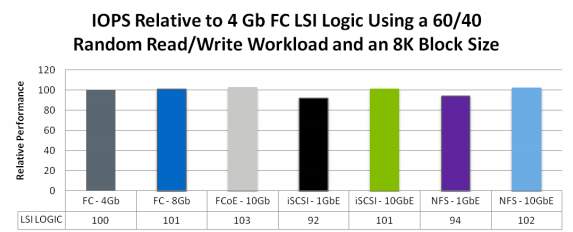
\includegraphics[width=\linewidth, keepaspectratio = true]{media/netapp_iops.png}
\mycaption{figure}{\label{abb:NetappIOPS}Netapp IOPS Durchsatz für alle unterstützten Protokolle im Vergleich zu 4Gb FC mit 8K Blockgrösse\cite{Jafri2011}}
\end{center}

Der Report von Netapp hat ebenfalls die Latenz verglichen. Bei der Latenz möchte man einen möglichst tiefen Wert erreichen. Gemäss \refabb{abb:NetappLatenz} ist die Latenz von iSCSI in einen 1 Gb Ethernet Netzwerk rund 9\% höher als bei Fibre Channel in einem 4Gb Netzwerk. Bei iSCSI in 10Gb Ethernet waren die Werte gleich gut wie Fibre Channel im 4Gb Netzwerk. Das Fibre Channel in einem 8Gb Netzwerk hatte jedoch rund 1\% tiefere Werte.\cite{Jafri2011}

\begin{center}
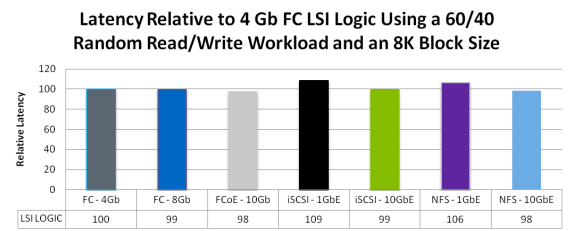
\includegraphics[width=\linewidth, keepaspectratio = true]{media/netapp_latence.png}
\mycaption{figure}{\label{abb:NetappLatenz}Netapp Latenz für alle unterstützten Protokolle im Vergleich zu 4Gb FC mit 8K Blockgrösse \cite{Jafri2011}}
\end{center}
 
\subsection{Logical Volume Manager}
Logical Volume Manager oder Dateisysteme, welche die Logik eines Logical Volume Managers kombinieren, ermöglichen mehrere Block-Geräte bzw. Logical Units zu einer grossen logischen Volume zusammenzufassen. Dies birgt den Vorteil, dass die maximale Grösse eines Block-Gerätes nicht der limitierende Faktor des darauf installierten Dateisystems ist. Neben dem Erstellen von Logischen Volumes können einige Logical Volume Manager den Last-Zugriff auf die verschiedenen Block-Geräte durch Striping optimaler verteilen und sorgen damit für eine besser Performance beim Datenzugriff. Eine weitere Aufgabe des Logical Volume Managers ist die redundante Haltung der Daten durch Spiegelung. Mittels serverseitiger Spiegelung (Host-Based Mirroring) können die Daten von zwei Standorten zur Verfügung gestellt werden. Dazu werden von zwei Speichersystemen, welche an unterschiedlichen Standorten installiert sind, gleich viele und gleich grosse Logical Units über das SAN dem Computersystem zugeteilt.

Klassische Server Linux Distributoren, wie Red Hat, Suse und Debian inkl. Ubuntu liefern den quelloffenen Logical Volume Manager 2 (LVM2) in ihrem Distributionspacket mit. Der LVM2 kann theoretisch auf einem 64-Bit System eine Logical Volume von 8 Exabyte bilden und adressieren. \cite{Levine2009}

Das ursprünglich von Oracle als ZFS-Ersatz entwickelte Btrfs Dateisystem könnte sich künftig zum Standard Dateisystem für viele Linux Server Distributionen mausern. Das für Solaris entwickelte ZFS als auch Btrfs kombinieren Dateisystem und Logical Volume Manager. Btrfs selbst wurde jedoch noch nicht als stabile Version veröffentlicht und ist deshalb für den produktiven Betrieb noch nicht empfehlenswert. \cite{Redler2011}


\subsection{Datei System}
Betriebssysteme adressieren die Daten auf Block-Geräten nicht direkt an, sondern greifen über das darüberliegende Dateisystem zu. Das Dateisystem organisiert wie und wo Dateien auf den Block-Geräten abgelegt werden und verwalten die freie Speicherkapazität. Einige Dateisysteme regeln auch die Zugriffsberechtigungen auf die Daten. Die Block-Geräte (Logical Units) können im SAN oder DAS an verschiedene Computersysteme gleichzeitig zugeteilt werden. Es ist die Aufgabe des Dateisystems sicherzustellen, dass mehrere Computersysteme gleichzeitig vom gleichen Dateisystem lesen bzw. auf dieses schreiben können. Konventionelle Dateisysteme wie Ext3 unter Linux gehen von einer exklusiven Nutzung des Speichers aus. Dieses Dateisystem enthält keine Funktionen, die den gleichzeitigen Zugriff auf Daten regeln. Problematik beim gleichzeitigen Zugriff ist die Sicherstellung der Datenkonsistenz. Schreiben zum Beispiel zwei Computersysteme gleichzeitig in dieselbe Datei, ist zu regeln, welche Änderung gültig ist, um Dateninkonsistenz zu vermeiden. Dateisysteme, welche den gleichzeitigen Datenzugriff erlauben, regeln den Zugriff auf Dateien z.B. mit einem Sperrmechanismus (locking). Schreibt ein Computersystem in eine solche gleichzeitig benutzte Datei, wird die Datei für Änderungen durch das andere Computersystemen gesperrt. Dieser muss sich den neuen aktuellen Stand mit einem Daten-Refresh wieder holen. Cluster Dateisysteme wie Red Hat Global Filesystem (GFS) und Red Hat Global Filesystem 2 (GFS2) unterstützen dieses Sperren. Das Dateisystem Red Hat GFS Version 2 unterstützt bei einem 64-bit-System theoretisch Dateisysteme bis 8 Exabyte, Red Hat gewährleistet jedoch nur einen Support von maximal 100 Terabyte. \cite{Levine2011}

Dateisysteme wie ZFS und Btrfs stellen die Integrität der Daten vor Veränderung, wie dies zum Beispiel durch einen Bit-Fehler auf dem Block Gerät oder im Memory entstehen könnte, mittels Prüfsumme sicher. Dabei wir zur jeder Datei eine Hash-Prüfsumme abgespeichert. Wird die Datei gelesen, wird die Prüfsumme aus der Datei neu berechnet und mit der abgespeicherten Prüfsumme verglichen. Sofern das Dateisystem ebenfalls gespiegelt ist, korrigiert das Dateisystem die fehlerhafte Datei aus der intakten Kopie automatisch. Dieses Verfahren wird auch als selbstheilend (self-healing) bezeichnet. \cite{Bonwick2005}\cite{Oracle}

Dateisysteme können mittels Sicherungssoftware auf Bandlaufwerke oder andere Speichermedien gesichert werden.


\section{Datei-Basierend}
Bei Datei-basierten Speicherarchitekturen werden Daten nicht wie bei Block-basierten Speicherarchitekturen über Blocke adressiert, sondern über Dateien.

Mit dem Aufkommen von Desktop-Computern, wurde die Rechenlast des zentralen Mainframecmputer wesentlich entlastet (verteilte Rechenlast auf viele kleine Rechner). Ohne die Vernetzung der Desktop-Computer mussten die Daten mittels portablen Speichermedien ausgetauscht werden. Dies mag in kleinen Umgebungen noch praktikabel gewesen zu sein, wurde jedoch mit der steigenden Anzahl der Teilnehmer zusehends schwieriger bis unmöglich. Verfügbarkeit und Konsistenz der Daten konnte nicht zufriedenstellend gelöst werden. Die direkte Vernetzung der Desktop-Computer erlaubte zwar den effizienten Datenaustausch über das Netzwerk, bot aber trotzdem keine gefällige Lösung für die Datenkonsistenz und Datensicherung. Die bessere Lösung war der gemeinsame zentral angelegte Speicher, in welchem sämtliche Unternehmensdaten für alle Benutzer verfügbar gehalten und mit einem regelmässigen Backup gesichert wurden. Alle Anwender verfügten immer über die aktuellste Version der Daten. Unternehmen wie Sun Microsystem, IBM, Microsoft und Apple erkannten die Bedürfnisse der Benutzer und entwickelten für ihre Betriebsysteme die Funktionen für den geteilten Datenzugriff.

Zu den bekanntesten und weitverbreitesten Lösungen zählen NFS und \gls{CIFS} (SMB).


\subsection{Network File System}
Das ursprünglich rein von der Firma SUN Microsystems (heute Oracle) 1984 entwickeltes Network-File-System, ermöglicht den gemeinsamen Zugriff von mehreren Computersystemen auf das Dateisystem eines zentralen Host (Server), als ob der einzelne Benutzer Zugriff auf ein lokales Dateisystem hat. Die zweite Version von NFS erschien 1989 und war die erste Version welche von Internet Standard Request for Comments (\gls{RFC}) standardisiert wurde und unter der \gls{RFC} Nummer 1094 \footnote{\url{http://tools.ietf.org/html/rfc1094}} veröffentlicht wurde. Für den Transport des NFS Protokolls wurde bis Version zwei ausschliesslich das \gls{UDP} Transportprotokoll unterstützt.
Die Version 3 von NFS (\gls{RFC} 1813)\footnote{\url{http://tools.ietf.org/html/rfc1813}}, die 1995 veröffentlicht wurde, war die erste Version, in der Computer, Betriebsystem, Netzwerk-Architektur und Transport-Protokoll unabhängig ist. Die Unabhängigkeit wird mit der Verwendung von Remote Procedure Call (\gls{RPC}) erreicht, welches wiederum ein eXternal Data Representation (\gls{XDR}) verwendet. \cite{Stern2001}

\begin{center}
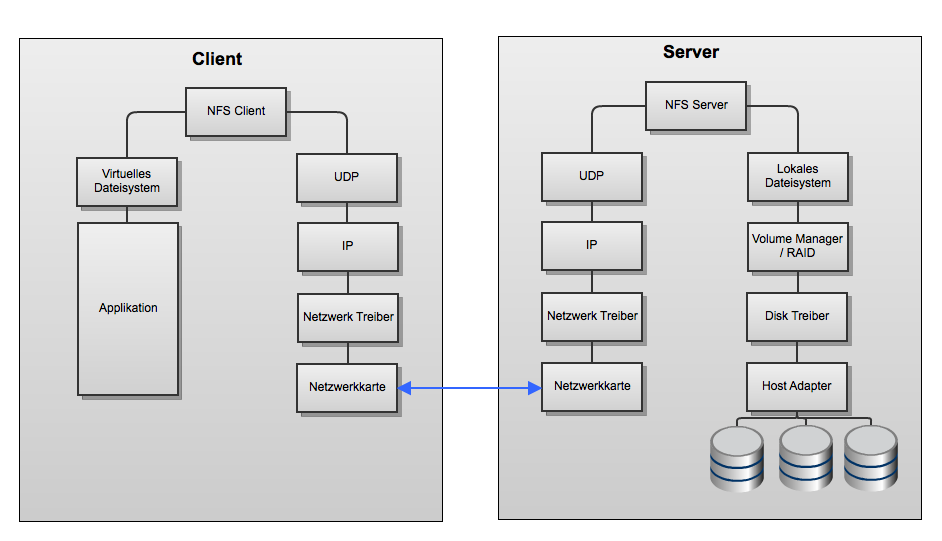
\includegraphics[width=\linewidth, keepaspectratio = true]{media/NFS.png}
\mycaption{figure}{\label{abb:NFSArchitektur}NFS Architektur \cite{Jafri2011}}
\end{center}

Wie im \refabb{abb:NFSArchitektur} zu entnehmen ist, ist NFS eine weitere Schicht, welche auf dem Dateisystem und dessen Block-Geräten des Computersystems bzw. Speichersystem aufbaut. So ist es zum Beispiel die Aufgabe des Dateisystems bzw. des Block-Gerätes, die Redundanz und Integrität der gespeicherten Daten sicherzustellen. 

Die Datenkonsistenz für den gleichzeitigen Zugriff von mehreren Computern stellt NFS mit einem separaten Protokoll, dem Network-Lock-Manager (NLM) sicher. Der Network-Lock-Manager sorgt dafür, dass eine Datei, welche von einem Computersystem geändert wird, vor der Änderung durch andere Benutzer, gesichert ist. Wenn ein Client eine Sperrung angefordert hat, muss derselbe Client dem Server die Entsperrung mitteilen, nachdem er die Daten nicht mehr benötigt. Diese Sperrlogik führt jedoch zu Problemen, wenn der Client vor der Entsperrung ein Systemabsturz erleidet, also die Entsperrung gar nicht mehr melden kann und somit die Datei für alle anderen Benutzer gesperrt bleibt.
NFS setzt mit NLM das Advisory Locking Sperr-Verfahren ein. Das bedeutet, dass andere Clients beim Zugriff auf eine gesperrte Datei nur darauf hingewiesen werden, dass die Datei gesperrt ist, ohne den Client daran zu hindern, eine gewünschte Änderung an den Daten vorzunehmen. \cite{Stern2001}

Seit Version 4 von NFS Protokoll (\gls{RFC} 3530) ist das Sperrverfahren (Locking) im Protokoll selber implementiert. Dadurch entfällt der zusätzliche Einsatz des Network Lock Managers. NFS Version 4 unterstützt zudem das Sperren eines Bytes-Bereiches innerhalb einer Datei. Der Client erhält vom Server lediglich einen Leasing-Zeitraum für die Sperrung (Lock), welche der Client vor Ablauf der Frist wieder erneuern muss, um sie aufrechtzuerhalten. NFS in der Version 4 erlaubt ferner das Sperrverfahren Mandatory Locking, das allen anderen Clients nicht ermöglicht, sich über die Sperrung hinwegzusetzen. \cite{Callaghan2003}

Indem NFS auf TCP/IP als Kommunikationsprotokoll aufbaut, kann eine NFS Freigabe, Standort übergreifend festgelegt werden. Es gilt auch hier, dass die Latenz und die Bandbreite der Verbindung zwischen den Standorten entscheidend ist und limitierend wirken kann.

NFS selbst hat keine eigene Implementierung für die Sicherstellung der Datenintegrität. Stattdessen verlässt sich NFS seit Version 2 auf die TCP und Ethernet Fehlererkennung. TCP prüft im Standardverfahren die Integrität mit einer 16-Bit-Integer Prüfsumme. Die 16-Bit-Integer Prüfsumme erkennt Fehler im pseudo IP-Header, TCP-Header und Daten. Das Verfahren zeigt Schwächen bei einzel Bit-Fehlererkennung. Ethernet verwendet für die Fehlererkennung eine CRC32 Prüfsumme. Diese ist zwar effektiv in der Erkennung und Behebung von Bit-Fehlern, bietet aber keinen durchgehenden (End-to-End) Schutz. Grund dafür ist beim Wechseln der Kollisionsdomäne-Paketes, wie es bei einen Swtich oder Router der Fall ist, da jedes Mal eine neu CRC32 Prüfsumme erstellt wird. Bei NFS ab Version 4 kann der Datentransfer zusätzlich mit Kerberos abgesichert werden. Kerberos hat einen strengen Schutz gegen Manipulationen am Datenpaket und stellt somit die Integrität der Daten sicher. Nachteilig ist nur, dass Kerberos zusätzlich eingerichtet werden muss. \cite{JohnL.202}

Bis und mit Version 4 war die Verarbeitung der Metadaten und die Verarbeitung der Daten in einem Protokoll und Server implementiert. NFS skalierte deshalb bei der Verarbeitung von Dateien mit grossem Speicherplatzbedarf nicht ausreichend. Fragt ein NFS-Client einen NFS-Server für eine Datei an, prüft der Server die Metadaten. Die Metadaten geben Auskunft über den Speicherort, die Grösse, das Erstellungsdatum und das Änderungsdatum einer Datei und wandelt die Anfrage in einen Disk I/O um. Die Daten der Datei werden gesammelt und über das Netzwerk übertragen. Bei kleinen Dateien benötigt der Server den grössten Zeitanteil für das Sammeln der Daten, während bei grossen Dateien der Transfer der Daten über das Netzwerk selbst der limitierende Faktor ist.
Mit der Entwicklung von pNFS konnte der Transfer der Daten parallelisiert werden. Die Architektur von NFS wurde dazu in mehrere Komponenten aufgeteilt. Der NFS Server besteht neu aus einem getrennten Metadaten Server und einem oder mehreren Daten-Servern. Die Aufgabe des Metadatenservers besteht darin, Ort und Art der Datenspeicherung zu verwalten. Die Daten-Server hingegen kümmern sich um Lese- und Schreibanfragen von den Clients.
Bei einer Anfrage für eine grosse Datei können mehrere Daten-Server parallel Teile der Datei dem Client ausliefern. Der Client kann dann die verschiedenen Teile wieder zu einer ganzen Datei zusammensetzen. \cite{Shepler2010}\cite{Group2010}

Mit der NFS Version 4.1 wurde pNFS Bestandteil von NFS und ist seit 2010 im \gls{RFC} 5661 standardisiert. Server Linux Distributoren, wie Red Hat haben vorerst NFS 4.1, erst als Vorschau in ihre Distribution integriert. \cite{EastJacquelynnMichaelHidep-Smith2011}




\subsection{NAS Appliance}

Network Attached Storage (NAS) sind Speichersysteme mit einem angepassten Dateisystem für den gemeinsamen Dateizugriff in einer heterogenen Computer Netzwerkumgebung, welche über ein LAN angeschlossen sind. Als Speicher verwenden NAS je nach Typ interne Festplatten, Direct Attached Storage oder einen über SAN angefügten Speicher.
An Clients stellen NAS den Speicher über NFS, CIFS, ISCSI zur Verfügung. High-End NAS können den Speicher auch über Fibre-Channel zur Verfügung stellen.

Gemäss Gartner gehören die Anbieter \gls{IBM}, \gls{EMC} und NetAPP zu den führenden NAS Anbietern im Midrange und High-End-Bereich. Gemäss Garnter gehört Magic Quadrant Netapp zusammen mit EMC zu den innovativsten Anbietern.

\begin{quotation}
\em 
\textbf{Strengths}
\begin{itemize}
\item NetApp remains one of the few truly unified storage providers among all top-tier vendors, with its software features continuing to be industry benchmarks. The company was able to regain some of the NAS revenue market share that it had lost in 2009. Its fast revenue growth in 2010 was driven by its successful campaign targeted at midsize enterprises with the value propositions of NFS supporting VMware and unified storage in consolidating Windows application storage.

\item In 2010, NetApp increased its aggregate up to 100TB with Data ONTAP 8.0.1 and introduced compression to complement its popular deduplication capability. It added a RESTful object storage interface (based on its acquisition of Bycast) to its unified storage, targeting global content repositories. On the hardware side, it launched new systems with better performance and denser disk shelves.

\item NetApp's new software bundles have simplified the procurement process and made software pricing more affordable. For customers seeking converged infrastructure, NetApp launched FlexPod for VMware with its partners Cisco and VMware, offering packages including servers, storage and switches.
\end{itemize}
\textbf{Cautions} 
\begin{itemize}
\item The vast majority of the Data ONTAP 8.0 adoption was on the 7 mode (instead of the cluster mode) for larger aggregates, while the early adoption of the cluster mode focuses on high- performance NFS file services. The cluster mode is not ready for mainstream enterprise customers who require those 7-mode features that are still missing in the cluster mode. The ONTAP 8.1 scheduled for release later this year will likely continue to support the two modes: clustered and nonclustered modes of operation.
\item While NetApp continues to enjoy its leading edge in unified storage, it's facing fiercer competition in the high-end NAS market, where file systems larger than 100TB are required and where high performance without the expensive Flash Cache is desired.
NetApp is also challenged in the low-end NAS and unified storage market with new products from both major and emerging competitors.
\end{itemize}
\end{quotation}\cite{RogerW.CoxPushanRinnenStanleyZaffos2011}


\section{Objekt-Basierend}

\subsection{Verteilte Dateisysteme}
Verteilte Dateisysteme sind Dateisysteme, welche ihren Speicher aus dem Speicher von mehren Computersysteme bilden. Somit werden die Daten auf mehre Computersysteme verteilt gespeichert, meist geschieht diese Redundant, dass heisst die Daten werden mehrfach auf Verschiedenen Computersysteme abgelegt um den Datenverlust beim Ausfall eines Computersystems zu vermeiden. Eines der bekanntesten Konzepte für Verteilte Dateisystem stammt von Google.

Unternehmen wie Google, welche Web-Applikationen mit Millionen von Anwendern betreiben und einen Speicherbedarf von hunderten Terrabyte bis Petabyte an Daten haben, stellen naturgemäss höchste Anforderungen an das Speichersystem. Google hat deshalb für das eigene verteilte Dateisystem das sogenannte Google Filesystem entwickelt. Google hat beim Design des Dateisystems angenommen, dass es auf gewöhnlichen und günstigen Hardwarekomponenten installiert wird, welche des öfteren Komponentenfehler haben könnten. Der Ausfall von Komponenten wird nicht als Sonderfall behandelt, sondern ist die Norm. Ferner handelt es sich bei den gespeicherten Daten eher um riesige Dateien mit einer Grösse von 100 Megabyte bis Multi-Gigabytes. Die Auslastung wird primär durch zwei Arten von Lesevorgängen verursacht. Das Lesen eines ganzen Datenstroms und das regellose Lesen. Die Schreibbelastung wird durch grosse sequentielle Schreibvorgänge verursacht. Dateien werden erweitert oder modifiziert. Als Architektur hat Google einen Cluster bestehend aus einem einzigen Metadaten-Server und mehreren Chunksservern gewählt. Die Daten werden bei Google in Einheiten unterteilt, den sogenannten Chunks. Jeder Chunk erhält eine eindeutige Identifizierung. Die Chunks werden über mehrere Chunkserver repliziert (Redundanz), um die Ausfallsicherheit zu gewährleisten. Der Metadaten-Server speichert in seinem Arbeitsspeicher die Daten bestehend aus Namensraum, Berechtigung Informationen, die Zuordnung der Datei zu den Chunks und den Speicherort der Chunks. Google hat das eigene Dateisystem bis anhin nicht veröffentlicht, hat jedoch eine Studie über das Design und die Architekturprinzipien veröffentlicht. Einige der heute erhältlichen verteilten Dateisysteme, wie Hadoop Distributed Filesystem (HDFS) und CloudStore beruhen auf denselben Architekturprinzipien wie sie die Google Studie darstellt. \cite{Ghemawat2003}\cite{Across2008}\cite{Rao2011} 

Neben Google Konzept, gibt es auch Konzepte von anderen Organisationen wie z.B. Amazon, welches mit Ihren Objekt-Basierten Speicher genannt Amazon S3 einen Online Speicher Ihren Kunden anbietet. Amazon S3 ist auf die Speicherung von sehr grossen Datenmengen konzipiert. Mit OpenStack Object Storage steht eine vergleichbare Quelloffene Alternative zu Amazon S3 zur Verfügung.

%!TEX root=../documentation-bachlorthesis-speicherarchitektur-lstucker.tex
\cleardoublepage
\chapter{Marktübersicht}

Dieser Abschnitt behandelt den Speichermarkt für primäre Speicher. Mit der Marktübersicht soll aufgezeigt werden, welche Speicherlösungskategorien in welchen Marktsegmente gefunden werden können und welche Hersteller sich im Markt etabliert haben. Zudem wird in einem kurzen Überblick dargestellt, welche Trends im Speichermarkt aktuell sind.

\section{Speicherlösungen}
Die erhältlichen Speicherlösungen lassen sich in die folgenden Kategorien aufteilen: 
\begin{itemize}
\item Konsumer Speicher
\item NAS Speicher
\item Modulare Disk Array Speicher
\item Verteilte Dateisystem Cluster Speicher 
\item Online Speicher auch Cloud Storage genannt.
\end{itemize}

\paragraph*{Konsumer Speicher}
Unter diesem Begriff werden die Speicher für Konsumer Elektronik, wie Notebook, PC, Smartphones, Mulitmedia Center, Audio Player, Camcorder usw. verstanden. Der Speicher basiert vorwiegend auf Blockgeräten wie Festplatten, Flash Disks, Solid State Disk etc.

\paragraph*{NAS Speicher}
NAS Produkte sind gemäss Gartner Speichersysteme, welche mit optimierten Dateisystemen gemeinsamen Dateizugriff für die im LAN angeschlossenen heterogenen Computer Systeme ermöglichen. Die NAS Produkte können ihren Speicher von internen Disks oder Direct-Attached Storage sowie von SAN Array Speicher zur Verfügung stellen. Die NAS Produkte verwenden für den gemeinsamen Dateizugriff Industrie Standardprotokolle, wie zB. Network File System (NFS) in Unix Umgebungen, oder Common Internet File System (CIFS) für Windows-Umgebungen. 
Viele NAS Produkte unterstützen heute natives ISCSI und in einigen Fällen Fibre Channel, um den Speicher auch über Logical Units zur Verfügung zu stellen. Die NAS Produkte werden mit einem für ihre Aufgaben optimierten Betriebsystem betrieben. \cite{RogerW.CoxPushanRinnenStanleyZaffos2011}

\paragraph*{Modulare Disk Array Speicher}
Modulare Disk Array Speicher sind Speichersysteme mit doppelten Controllern oder Node Cluster Architektur, welche den Speicher über Block Zugriffsprotokolle wie Fibre Channel oder ISCSI zur Verfügung stellen. Sie werden mit vom Hersteller vorkonfigurierten Festplatten ausgeliefert. Die Festplatten werden mit eigener Konfiguration oder mittels Konfiguration des Herstellers für die gewünschte Redundanz im Speichersystem in RAID-Einheiten zusammengefasst. Die Modularen Disk Arrays werden vorwiegend im SAN, manchmal auch im DAS Bereich eingesetzt.

\paragraph*{Verteilte Dateisystem Cluster Speicher}
Verteilte Dateisystemspeicher sind Speicher Cluster, welche den Speicher verteilt über mehrere handelsübliche Computerhardware zu einem grossen Speicher zusammenfassen und diese über eine API Anwendung zur Verfügung stellen. Die gespeicherten Daten werden meist in mehrfacher Redundanz über mehre Cluster Nodes im Speicher Cluster verteilt. Neben wenigen spezialisierten Anbieter werden die meisten verteilten Dateisystem Cluster-Speicher als individuelle Lösungen auf eigener Computer-Hardware betrieben.

\paragraph*{Online Speicher (Cloud Storage)}
Online Speicher, auch Cloud Storage genannt, wird von Gartner als Speichersystem beschrieben, welches seine verfügbare Kapazität über eine Wide-Area-Network inklusive dem Internet als Dienstleistung zur Verfügung stellt. Als Dienst ist die Speicherkapazität nach oben und nach unten skalierbar und wird nach dem jeweiligen Bedarf des Benutzers verrechnet. Dies ist mit der Versorgung von Strom durch einen Elektrizitätsversorger vergleichbar. \cite{AdamW.Couture2010}

\section{Marktsegment}
Der Speichermarkt kann in die Marktsegmente Heimanwender, Kommerz und Grossdatenanbieter unterteilt werden.

\paragraph*{Heimanwender/ Homeoffice} 
Der Heimanwender hat im Vergleich zu den anderen Marktsegmenten einen geringen Speicherbedarf. Seine Speicherlösungen beschränken sich in der Regel auf den internen Speicher seines Computersystems und seiner Elektronikgeräten. Für Heimanwender, welche einen etwas grösseren Speicherbedarf benötigen, (zum Beispiel Multimedia Inhalte oder Home Office) hat sich ein Markt für einfache NAS Systeme etabliert, welche in der Regel Speicherplatzgrössen bis zu 9 Tebibyte erlauben.


\paragraph*{Kommerz}
Zum Marktsegment 'Kommerz' gehören KMUs und Grossunternehmen in der Sparte Handel, Industrie und Dienstleitung. Diese Anbieter haben einen mittleren bis hohen Bedarf an Speicherkapazität, im Tebibyte Bereich. 

Unternehmen, welche tiefe Anforderungen an die eigene IT-Infrastruktur haben, verwenden ihre Speicherlösungen primär für den gemeinsamen Datenzugriff. 

%Dazu kommen oft NAS Speicherlösungen oder im Server integrierte Speicher zum Einsatz.

Unternehmen mit hohen Anforderungen an die eigene IT-Infrastruktur (z.B. Finanzdienstleister), verwenden ihre Speicherlösung für den gemeinsamen Datenzugriff auf Datenbanken und unstrukturierte Daten als hochverfügbare Systemumgebung.

%Die hochverfügbaren Systeme für den Betrieb von grossen relationalen Datenbanken, verwenden Modulare Disk Array Speicher, welche mittels Storage Area Network (kurz SAN) ihren Computersystemen redundant gesicherten Datenspeicher zur Verfügung stellt. Für den gemeinsamen Datenzugriff setzen diese Unternehmen ebenfalls auf NAS Speicherlösungen.

\paragraph*{Grosse Datenanbieter}
Zu den grossen Datenanbieter zählen Webdienstleister wie Google, Facebook, Yahoo, Amazone und Unternehmen aus der Multimedia Industrie wie Pixar Studios, RedBull, aber auch Forschungseinrichtungen wie Cern oder Bibliotheken wie die Amerikanische Library of Congress.
Diese verwalten in ihren Speichern grosse Datenvolumen im Bereich von mehreren hundert Tebibyte bis Exbibyte. 

Für die Speicherung solcher Datenmengen stützen sie sich auf verteilte Dateisystem Cluster Speicher oder hochleistungs NAS Speicherlösungen. 

\section{Gross Datenanbieter}
Gemäss den Anforderungen des Auftraggebers und den beshriebenen Szenarien zählt das zu evaluierende Speichersystem zum Marktsegment der Grossen Datenanbieter. Diese Arbeit und Marktanalyse beschränkt sich deshalb auf dieses Marktsegment.

Demzufolge beschäftigen wir uns mit Speicherlösungen in der Kategorie NAS Speicher, Modulare Disk Array Speicher, Verteilte Dateisystem Cluster Speicher und Online Speicher (Cloud Storage).

\section{Welche aktuellen Speicherlösungen konnten sich im Markt etablieren?}
\label{sec:MarktEtabliert}
%welche Systeme habe sich in jüngster Vergangenheit durchgesetzt und welcher Trend ist zu erwarten?

\paragraph*{NAS Speicherlösungen}
Gartner hat die Anbieter von NAS im mittleren und oberen Marktsegment auf deren Marktchancen hin untersucht. Gartner hat diese in Marktführer, Herausforderer, Visionäre und Nichen-Anbieter gegliedert. Es wurden nur Anbieter berücksichtigt, die NAS Lösungen ab einem Preis von 25'000 \$ anbieten, die mindestens eines der Protokolle NFS oder CIFS unterstützen und ein Betriebseinkommen von mindestens 5 Millionen Doller ausweisen. 

Als Marktführer wurden Anbieter, welche einen bedeutenden Marktanteil haben, ausreichend Marketing- und Verkaufs-Kapazitäten haben und technologisch führend und innovativ sind.

Als Herausforderer gelten Anbieter mit einem starken Produkt, welche einen namhaften Marktanteil besitzen und über Ressourcen verfügen, diesen ausbauen zu können. Die Anbieter sind jedoch zu wenig Visionär, um sich als Marktführer zu qualifizieren.

Als Visionäre gelten Anbieter, die ein einzigartiges, innovatives Produkte anbieten, welches operationale oder finanziell wichtige End-Benuzter Probleme anspricht, jedoch noch nicht bewiesen haben, einen substantiellen Marktanteil gewinnen zu können.

Als Nischen-Anbieter gelten Hersteller, welche clevere Produkte vermarkten, die auf kundenspezifische Bedürfnisse oder Marktsegmente ausgerichtet sind.

Wie aus der \refabb{abb:MagicQuaderNAS} zu entnehmen ist, stuft Gartner die NetApp dicht gefolgt von EMC als Marktleader ein. Als Herausforderer gilt Oracle und als Visionär gilt BlueArc.

Gartner sieht die Stärken von NetApp darin, dass dieser als einer der wenigen wirklichen Storage Anbieter alle Marktstufen abdeckt und mit Software-Features weiterhin die Messlatte der Industrie vorgibt. NetApp hat seinen Unternehmensgewinn in 2010 stark gesteigert. Zu deren Schwächen gehören, dass in der neuen Version ihrer Betriebsystem-Software noch nicht alle Funktionen von der alten Version integriert werden konnten, welche aber weitgehend zu den allgemein geforderten Features zählen.

Zu den Stärken von EMC zählt Gartner die Übernahme von Isilon's, einem visionären Anbieter, welcher starke Wachstumschancen im traditionellen Datencenter und im Cloud Service Markt hat. Gleichzeitig schwächt die Übernahme von Isilon den Hersteller, weil sich die Produkte nun den Funktionen und Einsatzgebieten überlappen und sich die Kunden fragen, wie der Fahrplan der künftigen Entwicklung aussieht, bevor der Kunde neue Investitionen tätigt.

Zu den Stärken von BlueArc zählt Gartner, dass BlueArc mit Titan und Mercury ein NAS System anbietet, welches hoch-performant und Modular ausbaubar ist. Zu den wichtigsten benötigten Verbesserungen gehören die ultraschnelle objektbasierte Replikation im Katastrophenfall. Als weitere Schwachstelle sieht Gartner zudem den kleinen Marktanteil.

\begin{center}
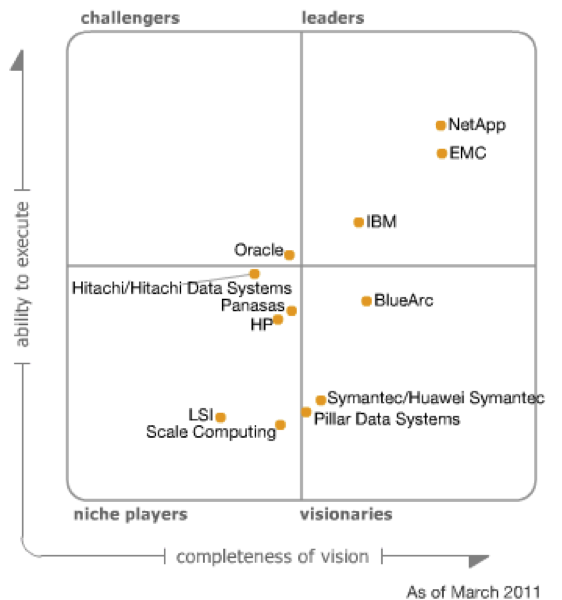
\includegraphics[, keepaspectratio = true]{media/magicquader_nas.png}
\mycaption{figure}{\label{abb:MagicQuaderNAS} Gartner Magic Quader März 2011}
\end{center}

\paragraph*{Modulare Disk Array Speicher}
Gartner hat die Anbieter von Modularen Disk Array im mittleren und oberen Bereich auf deren Marktchancen hin untersucht und hat diese in Marktführer, Herausforderer, Visionäre und Nichen-Anbieter unterteilt. Es wurden nur Anbieter berücksichtig die Modularen Disk Array Lösungen ab einem Preis von 25'000\$ anbieten und in den Märkten Nord Amerika, EMEA oder Japan und Asien Pazifik vertreten sind.

Als Marktführer wurden Anbieter, welche einen bedeutenden Marktanteil haben, ausreichend Marketing- und Verkaufs-Kapazitäten haben und technologisch führend und innovativ sind.

Als Herausforderer gelten Anbieter mit einem starken Produkt, welche einen namhaften Marktanteil besitzen und über Ressourcen verfügen, diesen ausbauen zu können. Die Anbieter sind jedoch zu wenig Visionär, um sich als Marktführer zu qualifizieren.

Als Visionäre gelten Anbieter, die ein einzigartiges, innovatives Produkte anbieten, welches operationale oder finanziell wichtige End-Benuzter Probleme anspricht, jedoch noch nicht bewiesen haben, einen substantiellen Marktanteil gewinnen zu können.

Als Nischen-Anbieter gelten Hersteller, welche clevere Produkte vermarkten, die auf kundenspezifische Bedürfnisse oder Marktsegmente ausgerichtet sind.

Wie aus der \refabb{abb:MagicQuaderModularDiskarrays} zu entnehmen ist, stuft Gartner EMC, NetApp, HP, Dell und Hitachi Data System zu den Marktführern ein. Oracle und Fujitsu sieht Gartner als Herausforderer und XIO wird als visionär bezeichnet.
 
\begin{center}
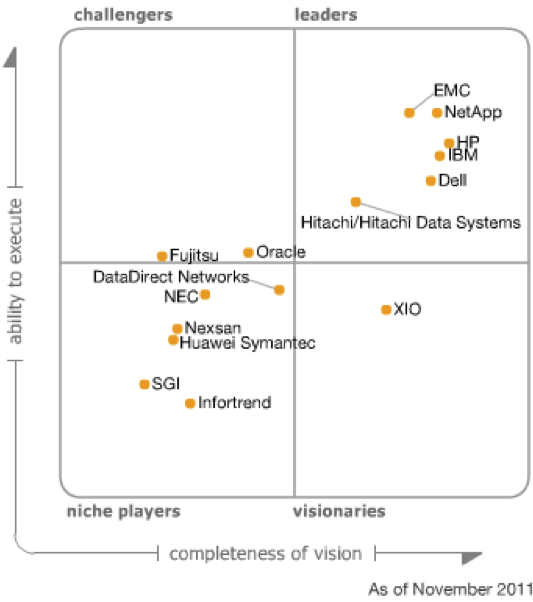
\includegraphics[, keepaspectratio = true]{media/magicquader_modulardiskarrays.png}
\mycaption{figure}{\label{abb:MagicQuaderModularDiskarrays} Gartner Magic Quader Modular Disk ArrayMärz 2011}
\end{center}


\paragraph*{Distributed Filesystem Cluster Speicherlösungen}
Zu den bekannten Vertreter der Distributed Filesystems gehören Hadoop HDFS, Gluster, Lustre. Alle drei haben gemeinsam, dass es sich bei den Lösungen um Open-Source Software handelt.

Hadoop basiert auf dem Design-Konzept von Google Filesystem und Google Mapreduce. The Guardian hat Apache Hadoop 2011 als Erfinder des Jahres ausgezeichnet. InfoWorld hat Hadoop für den InfoWorld 2012 Technology Award gewählt und für Gartner zählt Hadoop zu den top 10 Technologie-Trends, welche Einfluss auf die Informatik Infrastruktur nehmen. 
Zu dem prominentesten Unternehmen die Hadoop einsetzen und mitentwickeln zählen Yahoo und Facebook. Neben den beiden genannten gibt es mtllerweile viele weitere namhafte Unternehmen wie IBM, AOL, Twitter die Hadoop einsetzen. \cite{Guardian}\cite{Wayner2012}\cite{Casonato2012}\cite{Hadoop2012}

GlusterFS wurde von der Firma Gluster Inc. als Opensource Projekt entwickelt. Im Jahr 2011 wurde GlusterInc von der Firma Red Hat Inc. übernommen, um Lösungen für den Big Data Bereich anbieten zu können. Red Hat wurde mit der Übernahme von Gluster Inc zum Hauptunterstützer von GlusterFS.

\paragraph*{Online Speicher}
Zu den ersten grossen und wohl der bekannteste Online-Speicher Anbieter zählt Amazone mit ihrem S3 Produkt. Amazone veröffentlicht zwar keine Finanzdaten über ihre Cloud Produkte, hingegen veröffentlichte Amazon Daten bezüglich dem Wachstum der Anzahl gespeicherten Objekten. Gemäss eigenen Aussagen speicherte Amazon im Jahr 2006 ca. 2.9 Milliarden Objekte, im Jahr 2010 wahren es bereits 269 Milliarden Objekte. Dieses Ergebnis könnte Amazon im Jahr 2011 mit 762 Milliarden Objekten mehr als verdoppeln. \cite{Barr2012}

\begin{center}
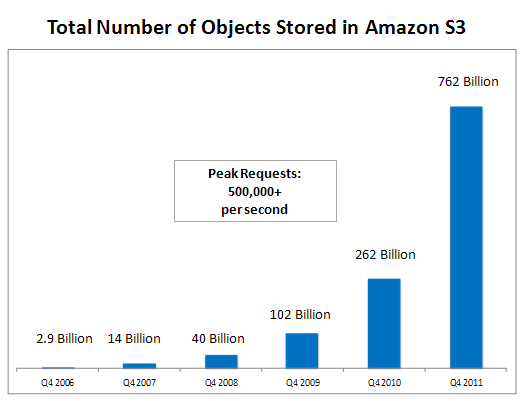
\includegraphics[, keepaspectratio = true]{media/s3_growth_2011_3.png}
\mycaption{figure}{\label{abb:AnzahlObjekteAmazonS3} 
\cite{Barr2012}Anzal gespeicherte Objekte in Amazon S3 \cite{Barr2012}}
\end{center}

Neben Amazon zählt RackSpace zu den führenden Cloud Anbietern. Wie Amazon bietet auch RackSpace den Online Speicher für jedermann an. Ihr Online Speicher wird unter der Produkt Bezeichnung Cloud File vermarktet. Hinter Cloud File steckt ein selbst entwickelter Speicher, OpenStack Object Storage mit Code Name Swift genannt. RackSpace hat an OpenStack Object Storage ein Jahr lang entwickelt und diese wie ihre anderen Cloud Eigenentwicklungen als Quelloffenes Projekt unter OpenStack veröffentlicht. Zu OpenStack tragen neben Rackspace weitere nahmhafte Unternehmen wie \gls{Dell}, \gls{HP}, Citrix, AMD, NetApp, Suse, AT\&T, NASA und andere bei.
RackSpace setzt ferner den selbst entwickelten OpenStack Object Storage als Online Speicher ein. \cite{OpenStack}

In der Schweiz ist die Entwicklung von Cloud Storage noch nicht so weit fortgeschritten wie in Amerika. Zu den wenigen Anbietern gehört unter anderem die Swisscom.


\section{Trend}
Für Gartner zählen Modular Disk Array Speicher und NAS zu den etablierten Speicherlösungen. Online Speicher (Cloud Storage) sieht Gartner eher als Speicherlösungen der Zukunft, welche sie laufend beobachtet und einen festen Platz in ihren Marktanalysen bekommen hat. 


%weshalb wiso warum

% wenig anbieter welche grosse datenanbieter 

% statistic massendaten
%!TEX root=../documentation-bachlorthesis-speicherarchitektur-lstucker.tex
\cleardoublepage
\chapter{Evaluation}

\section{Soll-Kriterien festlegen}
Die gewählten Kriterien für die Evaluation wurden zusammen mit dem Auftraggeber im Gespräch festgelegt. In einem weiteren Schritt wurden die einzelnen Kriterien nach ihrer logischen Zugehörigkeit hierarchisch geordnet und verfeinert (\refabb{abb:AHPKriterienbaum}). Die überarbeitete Kriterienauswahl wurde anlässlich eines weiteren Meetings mit dem Auftraggeber besprochen und fixiert. 

Die Kriterien sind für die späteren Verweise hierarchisch nummeriert.

\begin{center}
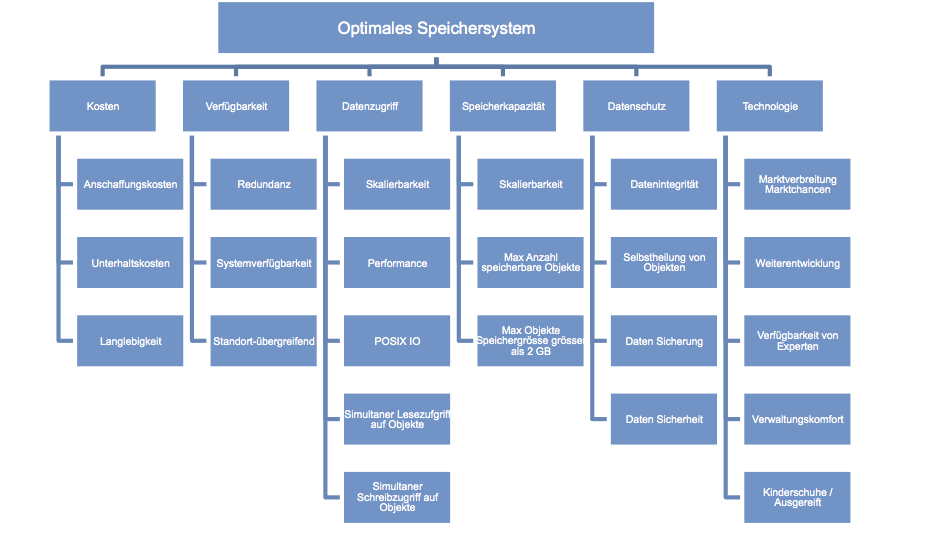
\includegraphics[width=\linewidth, keepaspectratio = true]{media/ahp_kriterienbaum.png}
\mycaption{figure}{\label{abb:AHPKriterienbaum} Optimales Speichersystem Kriterien}
\end{center}

\subsection{Haupt Soll-Kriterien festlegen}
Die Hauptkriterien sind in der obersten Hierarchie-Ebene dargestellt und werden durch ihre Unterkriterien weiter verfeinert und definiert.
\setcounter{paragraph}{0}
\renewcommand\theparagraph{Soll-\arabic{paragraph}}
\paragraph{Kosten}\label{Soll-1}
Die Kosten sollen einen gewinnbringenden Betrieb ermöglichen. 

\paragraph{Verfügbarkeit}\label{Soll-2}
Die Anforderungen an die Verfügbarkeit der Daten ist pro Szenario beschrieben und sollen entsprechend erfüllt werden. 

\paragraph{Datenzugriffe}\label{Soll-3}
Die Anzahl Datenzugriffe soll skalierbar sein. Es soll möglich sein, von mehreren Webservern gleichzeitig auf den Datenspeicher zugreifen zu können. Der Datenzugriff soll über POSIX IO oder über ein dokumentiertes API erfolgen können.

\paragraph{Speicherkapazität}\label{Soll-4}
Die Speicherkapazität soll die Speicheranforderungen der verschiedenen Szenerien erfüllen. Zudem soll die Speicherung von grossen Dateien bis zu 2 Gigabyte möglich sein.

\paragraph{Datenschutz}\label{Soll-5}
Der beschriebene Datenschutz soll jederzeit gewährleistet sein. Entscheidend ist der Schutz gegen die unerlaubte Veränderung von Daten. Für den Auftraggeber wichtig ist die laufende Sicherung der Daten, um den Verlust von Daten zu verhindern.

\paragraph{Technologie}\label{Soll-6}
Die Technologie bzw. das Produkt soll im Markt verbreitet sein, oder die Aussicht auf eine zukünftige Verbreitung im Markt. Zudem sollte die Technologie ausgereift sein, damit eine stabiler Betrieb gewährleistet ist. Nach Möglichkeit sollten genügen Experten verfügbar sein die sich mit der Technologie auskennen.

\subsection{Unter Soll-Kriterien festlegen}
Die Unterkriterien mit der gleichen Nummer-Ebene gehören zum selben Oberkriterium und werden später bei der Kriteriengewichtung untereinander direkt verglichen.

\setcounter{paragraph}{0}
\renewcommand\theparagraph{Soll-1-\arabic{paragraph}}

\paragraph{Anschaffungskosten}\label{Soll-1-1}
Die IT Infrastruktur soll über eine Abschreibungsdauer von 5 Jahren ausgelegt werden. Die gewählte Lösung kann sowohl eine Miete der Anlagen (Hosting) als auch die eigene Beschaffung der Hardware-Infrastruktur enthalten (managed servers). Um die Anbieter besser vergleichen zu können sind die Kosten auf 3 Jahre zu berechnen. 

\paragraph{Unterhaltskosten}\label{Soll-1-2}
Zu den Unterhaltskosten zählen sämtliche anfallenden Kosten für den Betrieb und Unterhalt der IT Infrastruktur eines Hosting-Anbieters. Nicht dazu zählen Kosten für die Anwendungs-Software (Anschaffung und Entwicklung) sowie die internen Kosten des Auftraggebers, sofern diese nicht direkt mit dem Betrieb der IT Infrastruktur verbunden sind (nicht direkt zurechenbare Kosten).

\paragraph{Nachhaltigkeit}\label{Soll-1-3}
Die Gesamtkosten (Anschaffung und Unterhalt) soll auf drei Jahre für alle Varianten gerechnet werden. Dabei soll auf eine gute Qualität der Komponenten für den Betrieb über 5 Jahre geachtet werden. Eine nachhaltige Planung steht im Vordergrund. Im Vergleich sollen sowohl die Anschaffungskosten und die Betriebskosten separat und auch insgesamt (TCO über 3 Jahre) verglichen werden.
Die Gesamtkosten sollten 50 \% der Einnahmen aus derselben Periode (3 Jahre) nicht übersteigen, damit ein langjähriger Betrieb wirtschaftlich realisierbar ist. Je tiefer die Gesamtkosten bei gleichbleibender Qualität, umso besser die Bewertung.

\setcounter{paragraph}{0}
\renewcommand\theparagraph{Soll-2-\arabic{paragraph}}

\paragraph{Redundanz}\label{Soll-2-1}
Die redundante Haltung von aktiven Daten, welche gelesen und manipuliert werden können, ermöglicht eine höhere Verfügbarkeit der Daten, z.B. beim Ausfall einer Systemkomponente. Die doppelte Datenhaltung wie sie bei der Datensicherung oder Archivierung entsteht, fällt nicht unter den Begriff "redundante Daten", da diese nicht direkt zur Erhöhung der Datenverfügbarkeit beiträgt. Die Speicherlösung sollte die Daten mindestens doppelt, oder wenn möglich dreifach redundant halten. 


\paragraph{Systemverfügbarkeit}\label{Soll-2-2}
Die verbesserte Systemverfügbarkeit, wird durch Software- oder Hardware-Redundanz erreicht. Die IT Infrastruktur (Server, Speicher, Netzwerk usw. soll möglichst redundant ausgelegt sein, um eine Verfügbarkeit nach AEC-3 Standard zu gewährleisten.

\paragraph{Standort-übergreifend}\label{Soll-2-3}
Die aktiven Daten sollen nach Möglichkeit an mindesten zwei voneinander getrennten Standorten gespeichert werden, um den Dienst auch im Falle des Ausfalls eines Rechenzentrums aufrecht erhalten zu können.

\setcounter{paragraph}{0}
\renewcommand\theparagraph{Soll-3-\arabic{paragraph}}

\paragraph{Skalierbarkeit}\label{Soll-3-1}
Die Speicherlösung sollte bei Bedarf den Speicher gleichzeitig an bis zu 30 Serversysteme zur Verfügung stellen können.

\paragraph{Performance}\label{Soll-3-2}
Die Speicherlösung soll eine IO-Performance von mindesten 27.31 MBit pro Sekunde haben.

\paragraph{POSIX IO}\label{Soll-3-3}
Die POSIX IO (inoffizielle Bezeichnung) ist ein Teil des POSIX Standards, welche die IO Schnittstelle für POSIX kompatible Applikationen definiert. Der Standard definiert ferner die Funktionen read(), write(), open(), close() inklusive deren Fehlerbehandlung. Die Speicherlösung soll für eine einfache Implementierung nach Möglichkeit diesen Standard unterstützen. 

\paragraph{Simultaner Lesezugriff auf Objekte}\label{Soll-3-4}
Das gleichzeitige Lesen desselben Objektes von zwei oder mehreren Serversystemen soll möglich sein.

\paragraph{Simulataner Schreibzugriff auf Objekte}\label{Soll-3-5}
Das gleichzeitige Schreiben auf dasselbe Objekte von zwei oder mehreren Serversystemen soll optional möglich sein.

\setcounter{paragraph}{0}
\renewcommand\theparagraph{Soll-4-\arabic{paragraph}}

\paragraph{Skalierbarkeit}\label{Soll-4-1}

\paragraph{Max Anzahl speicherbare Objekte}\label{Soll-4-2}
Das Speicherlösung soll die Anzahl der speicherbaren Objekte gemäss den Soll-Szenarien unterstützen. 

\paragraph{Max Objektgrösse von bis zu 2 GB}\label{Soll-4-3}
Das Speichersystem muss die Speicherung von Objekten mit einer Speichergrösse von bis zu 2 Gigabyte unterstützen.

\setcounter{paragraph}{0}
\renewcommand\theparagraph{Soll-5-\arabic{paragraph}}

\paragraph{Datenintegrität}\label{Soll-5-1}
Die Datenintegrität der gespeicherten Daten soll gewährleistet sein.

\paragraph{Selbstheilung von Objekten}\label{Soll-5-2}
Die Selbstheilung von beschädigten Daten soll nach Möglichkeit unterstützt werden. Diese Funktion ist bei der Verwaltung von grossen Datenmengen eine wichtige und geschätzte Funktion.

\paragraph{Datensicherung}\label{Soll-5-3}
Die gespeicherten Daten sollen mit einem effizienten Sicherungsverfahren gesichert werden können. Wenn die aktiven Daten nicht an zwei Standorten zur Verfügung gestellt werden können, wie in (\refsoll{Soll-2-3}) definiert, ist es zwingend erforderlich, dass der Sicherungsdatenträger an einem zweiten, physisch getrennten Standort gelagert wird.

\paragraph{Datensicherheit}\label{Soll-5-4}
Die Datenzugriffsberechtigung wird in der Applikation implementiert. Die Speicherlösung soll zudem sicherstellen, dass die Daten nicht von unerlaubten Dritten gelesen oder manipuliert werden können (physischer und logischer Zugriffsschutz).

\setcounter{paragraph}{0}
\renewcommand\theparagraph{Soll-6-\arabic{paragraph}}

\paragraph{Marktverbreitung / Marktchancen}\label{Soll-6-1}
Die Speicherlösung soll im Markt etabliert sein oder Tendenzen aufweisen, welche in den nächsten fünf Jahren die Verbreiterung im Markt wahrscheinlich erscheinen lässt.

\paragraph{Weiterentwicklung}\label{Soll-6-2}
Die Speichertechnologien, welche aktiv weiterentwickelt werden, sollen höher bewertet werden.

\paragraph{Verfügbarkeit von Experten}\label{Soll-6-3}
Die Verfügbarkeit von Experten einer etablierten Speicherlösungstechnologie soll sichtbar sein. Dabei soll das Expertenwissen regional breit verfügbar sein. Die Verfügbarkeit von Experten in der Schweiz ist höher zu werten als im Ausland.

\paragraph{Verwaltungskomfort}\label{Soll-6-4}
Die Speichertechnologie soll für die geforderte Datenmengen mit einem möglichst geringem Verwaltungsaufwand ermöglichen.

\paragraph{Kinderschuhe / Ausgereift}\label{Soll-6-5}
Die Speichertechnologie soll ausgereift und stabil laufen. Eine Implementierung von Beta-Versionen ist nicht erwünscht.

\section{KO-Kriterien}
Die KO-Kriterien sind Muss-Kriterien, welche von dem gewählten Speichersystem erfüllt werden müssen. Speichersysteme welche die KO-Kriterien nicht erfüllen, werden bei der AHP-Evaluation ausgeschlossen. Die KO-Kriterien wurde mit dem Auftraggeber besprochen und vereinbart.

\setcounter{paragraph}{0}
\renewcommand\theparagraph{KO-\arabic{paragraph}}

\paragraph{Dateigrösse bis 2 Gigibyte}\label{KO-1}
Die Speicherung von Dateien muss eine Objektgrösse von bis zu 2 Gibibyte erlauben.

\paragraph{Speicherkapazität Szenarien}\label{KO-2}
Die geforderten Speicherkapazitäten der Szenerien plus dem benötigten Speicherplatz für die Datenredundanz muss von der Speicherlösung unterstützt werden.

\paragraph{Kosten-Spannweite}\label{KO-3}
Die Kosten der teuersten Speicherlösung, darf nicht dreimal teurer sein, als die günstigste Lösung.

\section{Auswahl der Alternativen / Vertreter}
Mit dem Auftraggeber wurde definiert, dass für die Speicherlösungen, SAN, NAS, Distributed Filesystem Cluster, Online Speicher und dedizierter Webserver je ein Vertreter für die Evaluation ausgewählt werden sollen. Die Lösungen wurden nach Marktverbreitung und Technologie-Leader ausgewählt.

Die Alternativen/ Vertreter sind für die späteren Verweise nummeriert.

\setcounter{paragraph}{0}
\renewcommand\theparagraph{Al-\arabic{paragraph}}
\paragraph{Hetzner}\label{Al-1}
Dedizierte Webserver zählen im engeren Sinn nicht als reine Speicherlösungen. Der deutsche Hosting-Anbieter Hetzner bietet allerdings dedizierte Webserver mit der in Szenario 1 geforderten Speicherkapazität (siehe \refsec{Szenario-1}). Die bestehende Lösung wurde mit Hetzner Webserver realisiert. Hetzner als dedizierter Webserver Anbieter wurde deshalb auch berücksichtigt. 

\paragraph{NetApp NFS}\label{Al-2}
Als Vertreter für die NAS Speicherlösung wurde die NetApp FAS2240-4 gewählt. Für die Entscheidung zu NetApp haben dazu beigetragen, dass die Firma NetApp zu den Marktführern im NAS Bereich gehört und von Gartner als innovativ eingestuft wurde. Zudem pflegt die Firma ein breites Partnernetzwerk in der Schweiz.

\paragraph{NetApp iSCSI}\label{Al-3}
Als Vertreter für Block Speicherlösung wurde ebenfalls die NetApp FAS2240-4 gewählt. Die NetApp FAS2240-4 beherrscht ebenfalls iSCSI und FC SAN und kann somit als Block Speicherlösung ebenfalls eingesetzt werden. Für iSCSI im Vergleich zu FC-SAN spricht, dass neben der Ethernet-Netzwerk Technologie nicht zusätzliche Netzwerk Technologien eingesetzt werden müssen.

\paragraph{OpenStack Object Storage}\label{Al-4}

Als Vertreter für verteilten Speicher war ursprünglich Hadoop HDFS vorgesehen. In der aktuellen Version ist der Name-Node von HDFS noch ein Single Point of Failure (SPOF). Zudem liegen die Stärken bei HDFS bei den Datenprozessen für gespeicherte Objekte mittels MapReduce Algorithmus. Aus diesem Grund wurden weitere verteilte Dateisystem untersucht, wie etwa GlusterFS und OpenStack Object Storage. OpenStack Object Storage soll von der Architektur vergleichbar sein wie Amazon S3. Bei gewichtigen Online Speicheranbieter wird RackSpace erfolgreich eingesetzt. Ein weiterer Grund die für OpenStack Object Storage spricht, ist das gelungene quelloffene Projekt, das viele namhafte IT-Hersteller als Partner gewinnen konnte.

\paragraph{Amazon S3}\label{Al-5}
Amazon S3 wurde als Representant für Online Speicherlösungen gewählt. Amazon S3 ist gemäss \refsec{sec:MarktEtabliert} einer der etabliertesten Anbieter, wenn nicht die erfolgreichste Online Speicherlösung zur Zeit. Amazon betreibt mehrere Rechenzentrum verteilt auf mehrere Kontinenten. Für den Auftraggeber würde das Europäische Rechenzentrum in Frage kommen.


\subsection{Gewichtung der Soll-Kriterien mit AHP}

In diesem Abschnitt werden alle Soll-Kriteren der gleichen Hierarchie-Ebene bzw. gleichen Unter-Kriterien paarweise miteinander verglichen und mit der Skala \reftab{tab:9PBewertungsskala} aus dem \refchap{kab:Entscheidungsfindung} gewichtet.

% Vergleich mit Kosten
\paragraph*{\refsoll{Soll-1} verglichen mit \refsoll{Soll-2} (\ref{Soll-1}/\ref{Soll-2})} 
Mit steigenden Anforderungen an die Verfügbarkeit steigen auch die Kosten. Der Betrieb einer Infrastruktur eines Service-Anbieters muss kostendeckend sein. Einen Ausfall des Systems während definierten Betriebszeiten (das System muss online verfügbar sein), hat ebenfalls Auswirkungen auf das Unternehmen. So kann es zum Imageverlust, zu Kundenabgängen führen, oder die Zahlung von Entschädigungen erfordern. Die Rekonstruktion eines Datenverlustes kann trotz Sicherungskopie bei grossen Datenmengen zeitintensiv und kostspielig sein. Aus diesen Gründen ist ein gute Balance zwischen Kosten und Verfügbarkeit zu finden. Die Kosten sind deshalb im Vergleich zur Verfügbarkeit etwas grösser zu gewichten.

\textbf{Gewichtung: 3}

\paragraph*{\refsoll{Soll-1} verglichen mit \refsoll{Soll-3} (\ref{Soll-1}/\ref{Soll-3})}
Die Unterkriterien von Datenzugriffe sind mit der Skalierbarkeit der Datenzugriffe, Performance usw. wichtige Entscheidungskriteren. Dennoch sind diese im Vergleich zu den Kostenkriterien etwas tiefer zu gewichten. Grund dafür ist, dass der profitable Betrieb der Web-Applikation sichergestellt werden muss. Die Kosten sind deshalb etwas höher zu gewichten als die Datenzugriffe.

\textbf{Gewichtung: 3}

\paragraph*{\refsoll{Soll-1} verglichen mit \refsoll{Soll-4}}
Die Kosten und die Speicherkapazität sind gleich hoch bis etwas höher zu gewichten. Grund dafür ist, dass die Speicherlösung den rentablen Betrieb der Web-Applikation ermöglichen muss. Zugleich ist sicherzustellen, dass die geforderte Speicherkapazität vom Speichersystem erfüllt wird. Diese Kriterien sind deshalb gleich hoch zu gewichten.

\textbf{Gewichtung: 2}

\paragraph*{\refsoll{Soll-1} verglichen mit \refsoll{Soll-5}}
Für eine Web-Dienstleistung ist der Schutz der Daten wichtig. Wird die Plattform Opfer eines Hackersangriffes und wird dies publik, kann dies zu einem grossen Imageverlust führen. Aus diesem Grund ist sicherzustellen, das die Web-Applikation sicher betrieben werden kann. Die Sicherheit muss jedoch in erster Linie auf der Web-Applikation und dem Webserver sichergestellt werden und in zweiter Priorität auf dem Speichersystem. Die Kosten sind deshalb im Vergleich zum Datenschutz sehr viel bis absolut höher zu gewichten.

\textbf{Gewichtung: 8}

\paragraph*{\refsoll{Soll-1} verglichen mit \refsoll{Soll-6}}
Wie in den anderen Vergleichen ist sicherzustellen, dass die Web-Applikation rentabel betrieben werden kann. Deshalb sind möglichst tiefe Betriebskosten anzustreben. Die Kosten sind deshalb in Vergleich zur Technologie erheblich grösser zu gewichten.

\textbf{Gewichtung: 7}

% Vergleich mit Verfügbarkeit
\paragraph*{\refsoll{Soll-2} verglichen mit \refsoll{Soll-3}}
Aus Sicht des Anwenders ist die Verfügbarkeit der Daten höher zu gewichten als der möglichst schnelle Zugriff oder die Art und Weise wie der Zugriff stattfindet. Allerdings kann eine lange Wartezeit beim Ausliefern der Daten für den Anwender ebenfalls als "'nicht verfügbar"' empfunden werden. Es ist daher wichtig, dass der Zugriff auch vom Speichersystem effizient bewältig werden kann. Die Verfügbarkeit ist deshalb gleich bis etwas grösser zu gewichten als der Datenzugriff.

\textbf{Gewichtung: 2}

\paragraph*{\refsoll{Soll-2} verglichen mit \refsoll{Soll-4}}
Zum Geschäftsmodell der Web-Applikation gehört das Bereitstellung von Speicherkapazität für die Speicherung von grossen Bilddaten. Sind die Speicherkapazitäten ausgeschöpft und ist keine Wachstum mehr in der Speicherkapazität möglich, verliert der Auftraggeber ein neues Geschäft oder verliert gar einen bestehenden Kunden und kann mit dem Marktwachstum nicht Schritt halten. Aus diesem Grund ist die Verfügbarkeit etwas geringer zu gewichten als die Speicherkapazität.

\textbf{Gewichtung: 1/3}

\paragraph*{\refsoll{Soll-2} verglichen mit \refsoll{Soll-5}}
Um eine möglichst hohe Verfügbarkeit zu erreichen, werden zur Gewährleistung der Verfügbarkeit Massnahmen für den Datenschutz unternommen. Aus diesem Grund ist die Verfügbarkeit höher zu gewichten. 
Die Verfügbarkeit kann auch durch Schwachstellen erheblich höher zu gewichten sein als der Datenschutz.

\textbf{Gewichtung: 5}

\paragraph*{\refsoll{Soll-2} verglichen mit \refsoll{Soll-6}}
Für den Betrieb ist sicherzustellen, dass die Verfügbarkeit gewährleistet ist. Im Vergleich zur Marktverbreitung und die Verfügbarkeit von Experten ist deshalb die Verfügbarkeit erheblich bis sehr viel grösser zu gewichten.

\textbf{Gewichtung: 6}

% Vergleich mit Datenzugriffe
\paragraph*{\refsoll{Soll-3} verglichen mit \refsoll{Soll-4}}
Die Skalierbarkeit der Datenzugriff ist für ein Speichersystem fast gleich wichtig wie die Skalierbarkeit der Speicherkapazität. Die Art und Weise wie der Zugriff stattfindet, ist hingegen weniger wichtig als die maximale Grösse eines Objektes. Deshalb ist der Datenzugriff etwas weniger gross zu gewichten als die Speicherkapazität. 

\textbf{Gewichtung: 3}

\paragraph*{\refsoll{Soll-3} verglichen mit \refsoll{Soll-5}}
Für die Web-Applikation ist es wichtig, dass die geforderten Zugriffe auf das Speichersystem verarbeitbar sind. Die Sicherheit der Daten soll zudem vorwiegend aus Sicht der Applikation sichergestellt werden. Aus diesem Grund ist der Datenzugriff sehr viel grösser zu gewichten als der Datenschutz.

\textbf{Gewichtung: 7}

\paragraph*{\refsoll{Soll-3} verglichen mit \refsoll{Soll-6}}
Für die Web-Applikation ist es wichtig, dass die geforderten Zugriffe auf das Speichersystem verarbeitbar sind. Für den Langzeitbetrieb ist es aber auch wichtig, dass die Speichertechnologie mit den künftîgen Anforderungen des Marktes Schritt halten kann. Deshalb ist der Datenzugriff erheblich grösser zu gewichten als die Technologie.

\textbf{Gewichtung: 5}

% Vergleich mit Speicherkapazität
\paragraph*{\refsoll{Soll-4} verglichen mit \refsoll{Soll-5}}
Zum Geschäftsmodell der Web-Applikation gehört das Bereitstellung von Speicherkapazität zur Speicherung von grossen Bilddaten. Sind die Speicherkapazitäten erschöpft und ist kein Wachstum mehr möglich, kann der Auftraggeber mit den Marktanorderungen nicht mehr Schritt halten. Der Datenschutz der Daten ist ebenfalls wichtig. Der Schutz der Daten muss jedoch hauptsächlich auf der Applikationsseite erfolgen. Aus diesem Grund ist die Speicherkapazität sehr viel bis absolut grösser zu gewichten als der Datenschutz.

\textbf{Gewichtung: 8}

\paragraph*{\refsoll{Soll-4} verglichen mit \refsoll{Soll-6}}
Für den langfristigen Betrieb ist es wichtig, dass die Technologie laufend den neuen Marktanforderungen angepasst werden kann und genügend Experten vorhanden sind, welche mit der Technologie vertraut sind. Für das Geschäftsmodell ist es aber wichtiger, die notwendige Speicherkapazität zur Verfügung stellen zu können. Deshalb ist die Speicherkapazität sehr viel wichtiger als die Technologie.

\textbf{Gewichtung: 7}

% Vergleich mit Datenschutz
\paragraph*{\refsoll{Soll-5} verglichen mit \refsoll{Soll-6}}
Für den langfristigen Betrieb ist es wichtig, dass die Technologie laufend den neuen Marktanforderungen angepasst werden kann und genügend Experten vorhanden sind, welche mit der Technologie vertraut sind. Aus diesem Grund ist der Datenschutz etwas bis erheblich geringer zu gewichten als die Technologie.

\textbf{Gewichtung: 4}

\begin{table}[htbp]
\caption{AHP Gewichtung Top Kriterien}
\begin{tabular}{|l|r|r|r|r|r|r|r|}
\hline
\multicolumn{ 8}{|c|}{\textbf{Top Kriterien}} \\ \hline
 & \multicolumn{1}{l|}{\textbf{K}} & \multicolumn{1}{l|}{\textbf{V}} & \multicolumn{1}{l|}{\textbf{D}} & \multicolumn{1}{l|}{\textbf{S}} & \multicolumn{1}{l|}{\textbf{Ds}} & \multicolumn{1}{l|}{\textbf{T}} & \multicolumn{1}{l|}{\textbf{Gewicht}} \\ \hline
\textbf{Kosten (K)} & \textbf{1} & 3 & 3 & 2 & 8 & 7 & 0.353 \\ \hline
\textbf{Verfügbarkeit (V)} & 1/3 & \textbf{1} & 2 & 1/3 & 5 & 6 & 0.155 \\ \hline
\textbf{Datenzugriff (D)} & 1/3 & 1/2 & \textbf{1} & 1/4 & 7 & 5 & 0.122 \\ \hline
\textbf{Speicherkapazität (S)} & 0.5 & 3 & 4 & \textbf{1} & 8 & 7 & 0.299 \\ \hline
\textbf{Datenschutz (Ds)} & 1/8 & 1/5 & 1/7 & 1/8 & \textbf{1} & 1/4 & 0.026 \\ \hline
\textbf{Technologie (T)} & 1/7 & 1/6 & 1/5 & 1/7 & 4 & \textbf{1} & 0.045 \\ \hline
\textbf{Konsistenz Kennzahl} & 0.083 \\ \cline{1-2}
\end{tabular}
\label{AHPTop}
\end{table}

\subsubsection*{Gewichtung Kosten}

Wie nach der Gewichtung und in der \reftab{tab:AHPKosten} zu entnehmen ist, haben die Unterhaltskosten, gefolgt von Langlebigkeit die höhere Gewichtung als die Anschaffungskosten.

Die Paarvergleiche im Detail:

\paragraph*{\refsoll{Soll-1-1} verglichen mit \refsoll{Soll-1-2} (\ref{Soll-1-1}/\ref{Soll-1-2})}
Die Betriebskosten sind der Hauptkostenfakor in der Lebenszeit eines Informations-Systems. Gemäss Gartner fielen die weltweiten IT-Kosten im Jahr 2011 um 20 \% für Computer Hardware und um 43 \% für IT-Serviceleistungen. Zudem steigen die Kosten zum Beispiel von Disk Array Speicher nach Ablauf der ordentlichen vom Hersteller gewährleisteten Wartung, wegen teuren weiterführenden Wartungsverträge stark an.
Aus diesem Grund sind die Anschaffungskosten im Vergleich zu den Unterhaltskosten erheblich geringer zu gewichten.

\textbf{Gewichtung: 1/5}

\paragraph*{\refsoll{Soll-1-1} verglichen mit \refsoll{Soll-1-3} (\ref{Soll-1-1}/\ref{Soll-1-3})}
Fällt die Langlebigkeit eines Systems, weil es technologisch veraltet ist oder weil die Kosten für Wartungsverträge nach Ablauf der ordentlichen Wartung im Vergleich zur Neubeschaffung unrentabel sind, kurz aus. Sind erneut Kosten in der Anschaffung und Migration der Daten notwendig. Aus diesem Grund sind die Anschaffungskosten im Vergleich zur Langlebigkeit etwas geringer zu gewichten.

\textbf{Gewichtung: 1/3}


\paragraph*{\refsoll{Soll-1-2} verglichen mit \refsoll{Soll-1-3} (\ref{Soll-1-2}/\ref{Soll-1-3})}
Der Hauptkostenfakor in der Lebenzeit eines Informationssystems sind die Betriebskosten. Steigen diese Kosten aufgrund hoher Wartungvertragskosten mit der Lebenspanne des Systems an, kann sich der Betrieb als unrentabel herausstellen. Aus diesem Grund sind die Betriebskosten im Vergleich zur Langlebigkeit etwas grösser zu gewichten.

\textbf{Gewichtung: 3}

\begin{table}[htbp]
\caption{AHP Kosten}
\begin{tabular}{|l|r|l|l|l|}
\hline
\multicolumn{ 5}{|c|}{\textbf{Kosten}} \\ \hline
 & \multicolumn{1}{l|}{\textbf{A}} & \textbf{U} & \textbf{L} & \textbf{Gewicht} \\ \hline
\textbf{Anschaffung (A)} & 1 & \multicolumn{1}{r|}{0,2} & \multicolumn{1}{r|}{0,333} & \multicolumn{1}{r|}{0,105} \\ \hline
\textbf{Unterhaltskosten (U)} & 5 & \multicolumn{1}{r|}{1} & \multicolumn{1}{r|}{3} & \multicolumn{1}{r|}{0,637} \\ \hline
\textbf{Langlebigkeit (L)} & 3 & \multicolumn{1}{r|}{0,333} & \multicolumn{1}{r|}{1} & \multicolumn{1}{r|}{0.258} \\ \hline
\textbf{Konsistenz Kennzahl} & 0.033 \\ \cline{1-2}
\end{tabular}
\label{tab:AHPKosten}
\end{table}

\subsubsection*{Gewichtung Verfügbarkeit}

Wie nach der Gewichtung und in der \reftab{tab:AHPVerfügbarkeit} zu entnehmen ist, hat die Redundanz eine erheblich höhere Gewichtung als die Systemverfügbarkeit und Standortübergreifende Verfügbarkeit.

Die Paarvergleiche im Detail:

\paragraph*{\refsoll{Soll-2-1} verglichen mit \refsoll{Soll-2-2} (\ref{Soll-2-1}/\ref{Soll-2-2})}
Die Daten eines Informationssystem sind dessen wertvollstes Gut. Mit höherer Redundanz der Daten steigt auch die Verfügbarkeit der Daten.
Die Gesamtverfügbarkeit hängt jedoch auch von der Verfügbarkeit der einzelnen Systemkomponenten zusammen. Deshalb sollten die Daten systemübergreifend redundant sein, um ein hohe Verfügbarkeit zu gewährleisten. Gemäss eigener Erfahrungen ist die Zahl der Datenträgerausfällen höher als die restlichen Komponentenausfällen eines Systems. Die Datenredundanz ist deshalb erheblich grösser zu gewichten als die Systemredundanz.

\textbf{Gewichtung: 5}

\paragraph*{\refsoll{Soll-2-1} verglichen mit \refsoll{Soll-2-3} (\ref{Soll-2-1}/\ref{Soll-2-3})}
Die Standortübergreifende Verfügbarkeit der Daten kann nur mit Redundanz der Daten erreicht werden. Aus diesem Grund ist die Datenredundanz absolut höher zu gewichten als die standortübergreifende Verfügbarkeit.

\textbf{Gewichtung: 9}

\paragraph*{\refsoll{Soll-2-2} verglichen mit \refsoll{Soll-2-3} (\ref{Soll-2-2}/\ref{Soll-2-3})}
Die standortübergreifende Verfügbarkeit des System kann, erreicht werden, wenn die Daten auf mehrere Standorte verteilt werden und an diesen Standorten die Daten von einem lokalen System gelesen werden können. Das zweite System sollte idealerweise ein baugleiches Gerät sein, welches am zweiten Standort abgeschaltet ist und bei einem Ausfall am Hauptstandort hochgefahren wird.
Um die Verfügbarkeit zu gewährleisten, sollten keine manuellen Eingriffe erforderlich sein, da diese mit einem Unterbruch der Dienstleistung verbunden wäre. Aus diesem Grund ist die Systemverfügbarkeit etwas höher bis erheblich höher zu gewichten als die standortübergreifende Verfügbarkeit.

\textbf{Gewichtung: 4}

\begin{table}[htbp]
\caption{AHP Verfügbarkeit}
\begin{tabular}{|l|c|c|c|l|}
\hline
\multicolumn{ 5}{|c|}{\textbf{Verfügbarkeit}} \\ \hline
 & \multicolumn{1}{l|}{\textbf{R}} & \multicolumn{1}{l|}{\textbf{Sv}} & \textbf{St} & \textbf{Gewicht} \\ \hline
\textbf{Redundanz (R)} & 1 & 5 & \multicolumn{1}{r|}{9} & \multicolumn{1}{r|}{0,743} \\ \hline
\textbf{Systemverfügbarkeit (Sv)} & 1/5 & 1 & \multicolumn{1}{r|}{4} & \multicolumn{1}{r|}{0,194} \\ \hline
\textbf{Standort-Übergreifend (St)} & 1/9 & 1/4 & \multicolumn{1}{r|}{1} & \multicolumn{1}{r|}{0,063} \\ \hline
\textbf{Konsistenz Kennzahl} & 0,061 \\ \cline{1-2}
\end{tabular}
\label{tab:AHPVerfügbarkeit}
\end{table}

\subsubsection*{Gewichtung Datenzugriff}

Wie nach der Gewichtung und in der \reftab{tab:AHPDatenzugriff} zu entnehmen ist, hat die Fähigkeit für simultane Lesezugriffe auf Objekte dicht gefolgt von Skalierbarkeit der Datenzugriffe die höchste Gewichtung, gefolgt von Performance und der Unterstützung von POSIX IO. Die kleinste Gewichtung hat der simultane Schreibzugriff auf Objekte.


Die Paarvergleiche im Detail:

\paragraph*{\refsoll{Soll-3-1} verglichen mit \refsoll{Soll-3-2} (\ref{Soll-3-1}/\ref{Soll-3-2})}
Die Skalierung der Anzahl Datenzugriffe von mehreren Systemen ermöglicht die Web-Applikation höher redundant zu betreiben und die Verarbeitung der Bilddaten auf mehrere Server zu verteilen. Der maximale Datendurchsatz ist daher weniger bedeutend als dessen balansierten Verteilung der Zugriffe auf mehrere Server. Eine Speicherlösung, welche eine schlechte Performance aufweist, skaliert in der Regel ebenfalls nicht. Aus diesem Grund ist die Skalierung der Datenzugriffe etwas grösser zu gewichten als die Performance 

\textbf{Gewichtung: 3}

\paragraph*{\refsoll{Soll-3-1} verglichen mit \refsoll{Soll-3-3} (\ref{Soll-3-1}/\ref{Soll-3-2})}
Ist ein Zugriff auf die Daten über POSIX IO möglich, fällt allenfalls die Anpassung der entwickelten Web-Applikation geringer aus, als wenn er auf die Daten per API zugreifen muss. Für den Betrieb der Web-Applikation ist die Skalierung der Anzahl Datenzugriffe sehr viel bis absolut bedeutender als die Methode des Datenzugriffs.

\textbf{Gewichtung: 8}


\paragraph*{\refsoll{Soll-3-1} verglichen mit \refsoll{Soll-3-4} (\ref{Soll-3-1}/\ref{Soll-3-4})}
Der simultane Lesezugriff auf ein Objekt ermöglicht ein Objekt von mehreren Servern gleichzeitig zu lesen und dem Anwender darzustellen. Wird dies nicht unterstützt, kann dem Benutzer die Bilddatei nicht dargestellt werden, wenn ein anderer Besucher dieselbe Bilddatei gerade betrachtet. Aus diesem Grund ist die Skalierung und der simultane Lesezugriff auf Objekte gleich bedeutend.

\textbf{Gewichtung: 1}


\paragraph*{\refsoll{Soll-3-1} verglichen mit \refsoll{Soll-3-5} (\ref{Soll-3-1}/\ref{Soll-3-5})}
Der simultane Schreibzugriff auf ein Objekt erlaubt ein Objekt gleichzeitig von zwei oder mehreren Systemen bearbeiten zu können. Die Web-Applikation des Auftraggeber führt jedoch keine Änderungen an einer original Bilddatei durch, sondern erstellt modifizierte Kopien. Aus diesem Grund ist der gleichzeitige Schreibzugriff auf ein Objekt absolut geringer zu gewichten als die Skalierung des Datenzugriffs.

\textbf{Gewichtung: 9}

\paragraph*{\refsoll{Soll-3-2} verglichen mit \refsoll{Soll-3-3} (\ref{Soll-3-2}/\ref{Soll-3-3})}
Für den Betrieb der Web-Applikation ist die Performance der Datenzugriffe erheblich bis sehr viel bedeutender als die Methode des Datenzugriffs.

\textbf{Gewichtung 6}

\paragraph*{\refsoll{Soll-3-2} verglichen mit \refsoll{Soll-3-4} (\ref{Soll-3-2}/\ref{Soll-3-4})}
Die Performance ist erheblich geringer bedeutend als der simultane Lesezugriff auf Objekte. Grund dafür ist, dass das gleiche Objekte von mehreren Web-Servern gelesen werden kann, um diese den Website Besuchern darstellen können 

\textbf{Gewichtung: 1/5}

\paragraph*{\refsoll{Soll-3-2} verglichen mit \refsoll{Soll-3-5} (\ref{Soll-3-2}/\ref{Soll-3-5})}
Weil keine Manipulationen an der original Bilddatei durchgeführt wird, ist die Performance des Datenzugriff erheblich höher zu gewichten als der simultane Schreibzugriff auf Objekte. 

\textbf{Gewichtung: 5}


\paragraph*{\refsoll{Soll-3-3} verglichen mit \refsoll{Soll-3-4} (\ref{Soll-3-3}/\ref{Soll-3-4})}
Die Zugriffsmethode der Web-Applikation kann bei Bedarf durch die Entwickler angepasst werden. Für den Betrieb der Web-Applikation ist daher die Zugriffsmethode auf die Bilddaten erheblich geringer bedeutend als der simultane Lesezugriff.

\textbf{Gewichtung: 1/5}


\paragraph*{\refsoll{Soll-3-3} verglichen mit \refsoll{Soll-3-5} (\ref{Soll-3-3}/\ref{Soll-3-5})}
Weil keine Änderungen an original Bilddateien durchgeführt werden, ist es für den Auftraggeber bedeutender, dass ein Zugriff über POSIX IO möglich ist.

\textbf{Gewichtung: 3}


\paragraph*{\refsoll{Soll-3-4} verglichen mit \refsoll{Soll-3-5} (\ref{Soll-3-4}/\ref{Soll-3-5})}
Die Webapplikation des Auftraggeber führt keine Änderungen an der original Bilddatei durch, was den simultanen Schreibzugriff auf Objekten für den Betrieb der Web-Applikation von geringer Bedeutung ist. Der simultane Lesezugriff auf Objekten muss für den Betrieb der Web-Applikation möglich sein, damit die Bilddaten in mehreren Websitzungen gleichzeitig dargestellt werden können. Deshalb ist der simultane Lesezugriff gegenüber dem simultanen Schreibzugriff absolut höher gewichtet.

\textbf{Gewichtung: 9}

\begin{table}[htbp]
\caption{AHP Gewichtung Datenzugriff}
\begin{tabular}{|l|c|c|c|c|c|l|}
\hline
\multicolumn{ 7}{|c|}{\textbf{Datenzugriff}} \\ \hline
 & \multicolumn{1}{l|}{\textbf{SK}} & \multicolumn{1}{l|}{\textbf{Pe}} & \multicolumn{1}{l|}{\textbf{POI}} & \multicolumn{1}{l|}{\textbf{L}} & \multicolumn{1}{l|}{\textbf{S}} & \multicolumn{1}{l|}{\textbf{Gewicht}} \\ \hline
\textbf{Skalierbarkeit (Sk)} & 1 & 3 & 8 & 1 & 9 & 0,364 \\ \hline
\textbf{Performance (Pe)} & 1/3 & 1 & 6 & 1/5 & 5 & 0,158 \\ \hline
\textbf{POSIX IO (POI)} & 1/8 & 1/6 & 1 & 1/5 & 3 & 0,056 \\ \hline
\textbf{Simultaner Lesezugriff auf Objekte (L)} & 1 & 5 & 5 & 1 & 9 & 0,392 \\ \hline
\textbf{Simultaner Schreibzugriff auf Objekte (S)} & 1/9 & 1/5 & 1/3 & 1/9 & 1 & 0,031 \\ \hline
\textbf{Konsistenz Kennzahl} & 0,08 \\ \cline{1-2}
\end{tabular}
\label{tab:AHPDatenzugriff}
\end{table}

\subsubsection*{Gewichtung Speicherkapazität}


Wie nach der Gewichtung und in der \reftab{tab:AHPSpeicherkapazität} zu entnehmen ist, hat die Skalierbarkeit zusammen mit der max. Anzahl speicherbarer Objekte die höchste Gewichtung. Die Möglichkeit zur Speicherung von Objekte grösser als 2 GiB hat die tiefste Gewichtung, da die mindest Speichergrösse von bis zu 2 GiB bereits als KO Kriterium \ref{KO-1} festgelegt wurde und es sich somit um ein optionales Kriterium handelt.

Die Paarvergleiche im Detail:

\paragraph*{\refsoll{Soll-4-1} verglichen mit \refsoll{Soll-4-2} (\ref{Soll-4-1}/\ref{Soll-4-2})}
Die Skalierung der Speicherkapazität ist gleich zu gewichten wie die maximale Anzahl speicherbarer Objekte. Beides sind limitierende Faktoren, die bei erreichen der Grenze die Speicherung von neuen Objekten verunmöglichen. Erreicht man die Grenze der speicherbaren Objekten, kann die vorhandene freie Speicherkapazität nicht für neue Objekte verwendet werden. Umgekehrt wenn die Speicherkapazität nicht ausgebaut werden kann, kann die freie Kapazität an speicherbaren Objekten nicht dazu verwendet werden, neue Objekte zu speichern.

\textbf{Gewichtung: 1}

\paragraph*{\refsoll{Soll-4-1} verglichen mit \refsoll{Soll-4-3} (\ref{Soll-4-1}/\ref{Soll-4-3})}
Die Skalierbarkeit der Speicherkapazität ist für den Betrieb sehr viel höher zu gewichten als die maximale Speichergrösse für Objekte grösser als 2 Gigibyte.

\textbf{Gewichtung: 7}

\paragraph*{\refsoll{Soll-4-2} verglichen mit \refsoll{Soll-4-3} (\ref{Soll-4-2}/\ref{Soll-4-3})}
Die maximale Anzahl speicherbarer Objekte ist für den Betrieb sehr viel höher zu gewichten als die maximale Speichergrösse für Objekte grösser als 2 Gigibyte.

\textbf{Gewichtung: 7}

\begin{table}[htbp]
\caption{AHP Gewichtung Speicherkapazität}
\begin{tabular}{|l|c|c|c|l|}
\hline
\multicolumn{ 5}{|c|}{\textbf{Speicherkapazität}} \\ \hline
 & \multicolumn{1}{l|}{\textbf{S}} & \textbf{A} & \textbf{O} & \textbf{Gewicht} \\ \hline
\textbf{Skalierbarkeit (S)} & 1 & \multicolumn{1}{r|}{1} & \multicolumn{1}{r|}{7} & \multicolumn{1}{r|}{0,467} \\ \hline
\textbf{Max Anzahl speicherbare Objekte (A)} & 1 & \multicolumn{1}{r|}{1} & \multicolumn{1}{r|}{7} & \multicolumn{1}{r|}{0,467} \\ \hline
\textbf{Max Objekt Speichergrösse grösser als 2 GiB (O)} & 1/7 & \multicolumn{1}{r|}{1/7} & \multicolumn{1}{r|}{1} & \multicolumn{1}{r|}{0.067} \\ \hline
\textbf{Konsistenz Kennzahl} & 0 \\ \cline{1-2}
\end{tabular}
\label{tab:AHPSpeicherkapazität}
\end{table}

\subsubsection*{Gewichtung Datenschutz}

Wie nach der Gewichtung und in der \reftab{tab:AHPDatenschutz} zu entnehmen ist, hat das Kriterium Datensicherung gefolgt von Datenintegrität die höchste Gewichtung. Erheblich weniger Gewichtung haben Selbstheilung von Objekten und Datensicherheit.

Die Paarvergleiche im Detail:


\paragraph*{\refsoll{Soll-5-1} verglichen mit \refsoll{Soll-5-2} (\ref{Soll-5-1}/\ref{Soll-5-2})}
Damit das Speichersystem beschädigte Objekte selbständig heilen kann, ist es erforderlich, dass die Objekte redundant gespeichert werden und die Integrität der gespeicherten Objekte geprüft wird. Die Integrität der Objekte wird dabei mit einer zuvor erstellten und gespeicherten Hash-Prüfsumme verglichen. Aus diesem Grund ist die Datenintegrität erheblich höher zu gewichten als die Selbstheilung von Objekten.

\textbf{Gewichtung: 5}

\paragraph*{\refsoll{Soll-5-1} verglichen mit \refsoll{Soll-5-3} (\ref{Soll-5-1}/\ref{Soll-5-3})}
Verliert man alle primären Daten durch einen Hard- bzw. Software Fehler oder durch unerlaubtes Einwirken von Dritten, ist es unerlässlich, dass eine vollständige und konsistente Sicherungskopie der Daten besteht, um keinen totalen Datenverlust hinnehmen zu müssen.
Wenn ferner die Datenintegrität nicht sichergestellt ist, besteht ebenfalls die Gefahr eines Datenverlustes. Ist ein Objekt nicht mehr integer sondern korrupt und wird dies nicht vor der Datensicherung festgestellt, besteht die Gefahr eines Datenverlustes.
Der Verlust aller Daten ist schwerwiegender als der Verlust einzelner Daten.
Aus diesem Grund ist die Datenintegrität geringer zu gewichten als die Datensicherung.

\textbf{Gewichtung: 1/3}

\paragraph*{\refsoll{Soll-5-1} verglichen mit \refsoll{Soll-5-4} (\ref{Soll-5-1}/\ref{Soll-5-4})}
Primär muss bei einer Webapplikation die Datensicherheit innerhalb der Webapplikation sichergestellt werden. Aus diesem Grund ist die Datensicherheit sehr viel höher zu gewichten als die Datenintegrität.

\textbf{Gewichtung: 7}

\paragraph*{\refsoll{Soll-5-2} verglichen mit \refsoll{Soll-5-3} (\ref{Soll-5-2}/\ref{Soll-5-3})}
Die Selbstheilung von Daten stellt sicher, dass alle redundant gespeicherten Primären-Daten}integer sind. Durch die Selbstheilung verringert sich das Risiko des Datenverlustes. 
Der Verlust aller Daten ist jedoch schwerwiegender als der Verlust einzelner Daten.
Aus diesem Grund ist die Selbstheilung der Daten erheblich geringer zu gewichten als die Datensicherung.

\textbf{Gewichtung: 1/5}

\paragraph*{\refsoll{Soll-5-2} verglichen mit \refsoll{Soll-5-4} (\ref{Soll-5-2}/\ref{Soll-5-4})}
Primär muss bei einer Webapplikation die Datensicherheit innerhalb der Webapplikation sichergestellt werden. Aus diesem Grund ist die Selbsheilung der Daten etwas höher zu gewichten als die Datensicherheit.

\textbf{Gewichtung: 3}

\paragraph*{\refsoll{Soll-5-3} verglichen mit \refsoll{Soll-5-4} (\ref{Soll-5-3}/\ref{Soll-5-4})}
Die Datensicherheit ist primär auf der Web-Applikationschicht zu gewährleisten und zu realisieren. Erfährt man einen Datenverlust durch das Einwirken von Dritten, ist sicherzustellen, dass eine Sicherungskopie der Daten existiert. Aus diesem Grund ist die Sicherung der Daten sehr viel höher zu gewichten als die Sicherheit. 

\textbf{Gewichtung: 7}

\begin{table}[htbp]
\caption{AHP Gewichtung Datenschutz}
\begin{tabular}{|l|c|c|c|c|l|}
\hline
\multicolumn{6}{|c|}{\textbf{Datenschutz}} \\ \hline
 & \multicolumn{1}{c|}{\textbf{I}} & \multicolumn{1}{c|}{\textbf{H}} & \multicolumn{1}{c|}{\textbf{B}} & \multicolumn{1}{c|}{\textbf{S}} & \multicolumn{1}{l|}{\textbf{Gewicht}} \\ \hline
\textbf{Datenintegrität (I)} & 1 & 5 & 1/3 & 7 & \multicolumn{1}{r|}{0,311} \\ \hline
\textbf{Selbstheilung von Objekten (H)} & 1/5 & 1 & 1/5 & 3 & \multicolumn{1}{r|}{0,097} \\ \hline
\textbf{Datensicherung (B)} & 3 & 5 & 1 & 7 & \multicolumn{1}{r|}{0,544} \\ \hline
\textbf{Datensicherheit (S)} & 1/7 & 1/3 & 1/7 & 1 & \multicolumn{1}{r|}{0,048} \\ \hline
\textbf{Konsistenz Kennzahl} & 0,084 \\ \cline{1-2}
\end{tabular}
\label{tab:AHPDatenschutz}
\end{table}

\subsubsection*{Gewichtung Technologie}

Wie nach der Gewichtung und in der \reftab{tab:AHPTechnologie} zu entnehmen ist, hat das Kriterium Ausgereift mit Abstand die höchste Gewichtung. Die zweithöchste Gewichtung ist der Weiterentwicklung zugeordnet, gefolgt von der Verfügbarkeit von Experten und der Marktverbreitung/Marktchancen. Am wenigsten Gewicht wird dem Verwaltungskomfort zugeteilt.

Die Paarvergleiche im Detail:


\paragraph*{\refsoll{Soll-6-1} verglichen mit \refsoll{Soll-6-2} (\ref{Soll-6-1}/\ref{Soll-6-2})} Ein Technologie, die nicht mehr weiterentwickelt wird, hat trotzt einer allfälligen grossen Marktverbreitung über kurz oder lang keine Chancen und wird durch neuere und bessere Technologien aus dem Markt verdrängt. Beim Entscheid zu einer neuen Lösung ist es wichtig, dass man sich für ein Technologie entscheidet, welche noch nicht am Ende ihres Lebenszyklus angelangt ist. Aus diesem Grund ist die Marktverbreitung/Marktchance erheblich geringer zu gewichten als die Weiterentwicklung.

\textbf{Gewichtung: 1/5}


\paragraph*{\refsoll{Soll-6-1} verglichen mit \refsoll{Soll-6-3} (\ref{Soll-6-1}/\ref{Soll-6-3})}
Mit einer hohe Marktverbreitung ist in der Regeln die Verfügbarkeit von Experten ebenfalls gegeben. Aus diesem Grund ist die Marktverbreitung und die Verfügbarkeit von Experten gleich zu gewichten

\textbf{Gewichtung: 1}

\paragraph*{\refsoll{Soll-6-1} verglichen mit \refsoll{Soll-6-4} (\ref{Soll-6-1}/\ref{Soll-6-4})}
Ein Produkt welches hohen Verwaltungskomfort aufweist, jedoch wegen anderen Faktoren ein schlechte Marktverbreitung oder Marktchancen aufweist, ist für den langfristigen Betrieb eher ungeeignet. Die Marktverbreitung ist deshalb etwas höher zu gewichten als der Verwaltungskomfort.

\textbf{Gewichtung: 3}

\paragraph*{\refsoll{Soll-6-1} verglichen mit \refsoll{Soll-6-5} (\ref{Soll-6-1}/\ref{Soll-6-5})}
Für den Betrieb der Web-Applikation ist es wichtig, dass die Speicherlösung technisch und und im Alltagseinsatz ausgereift ist. Die Marktverbreitung ist deshalb absolut geringer zu gewichten als eine ausgereifte Speicherlösung.

\textbf{Gewichtung: 1/9}

\paragraph*{\refsoll{Soll-6-2} verglichen mit \refsoll{Soll-6-3} (\ref{Soll-6-2}/\ref{Soll-6-3})}
Eine Technologie, welche nicht mehr weiter entwickelt wird, lauft Gefahr, den Marktanforderungen bald nicht mehr zu genügen und könnte in der Folge von neuen Technologien ersetzt werden. Der Rückgang der Marktanteile der Technologie hat auch zur Folge, dass der Nachwuchs sich in den alten Technologien ebenfalls weiterbilden muss. Dies wiederum hat zur Folge, dass die Anzahl Experten mittelfristig ebenfalls abnimmt. Aus diesem Grund ist die Weiterentwicklung erheblich höher zu gewichten als die Verfügbarkeit von Experten.

\textbf{Gewichtung: 5}

\paragraph*{\refsoll{Soll-6-2} verglichen mit \refsoll{Soll-6-4} (\ref{Soll-6-2}/\ref{Soll-6-4})}

Die Weiterentwicklung ist für den Langzeitbetrieb wichtiger als der Verwaltungskomfort. Bestehende Schwächen im Verwaltungskomfort könnten in weiterentwickelten Versionen behoben oder verbessert sein. Die Weiterentwicklung wird deshalb für den Langzeitbetrieb sehr viel höher gewichtet als der Verwaltungskomfort.

\textbf{Gewichtung: 7}

\paragraph*{\refsoll{Soll-6-2} verglichen mit \refsoll{Soll-6-5} (\ref{Soll-6-2}/\ref{Soll-6-5})}
Für den Betrieb der Web-Applikation ist es wichtig, dass die Speicherlösung technisch und betrieblich ausgereift ist. Die Weiterentwicklung ist deshalb erheblich geringer zu gewichten als eine ausgereifte Speicherlösung.

\textbf{Gewichtung: 1/5}


\paragraph*{\refsoll{Soll-6-3} verglichen mit \refsoll{Soll-6-4} (\ref{Soll-6-3}/\ref{Soll-6-4})}
Bietet ein Speicherlösung einen hohen Verwaltungskomfort, kann die Verwaltung in der Regel schneller und von weniger gut geschultem Personal durchgeführt werden. Folglich verringert sich die Abhängigkeit zu Experten. Für die Konzeption, Inbetriebnahme, spätere Optimierung und Problemlösungen der Speicherinfrastruktur ist man in der Regel weiterhin auf das Wissen von Experten angewiesen. Aus diesem Grund ist es wichtig, dass der Zugriff auf Expertenwissen vorhanden ist. Die Verfügbarkeit von Experten ist deshalb, erheblich höher zu gewichten als der Verwaltungskomfort. 

\textbf{Gewichtung: 5}

\paragraph*{\refsoll{Soll-6-3} verglichen mit \refsoll{Soll-6-5} (\ref{Soll-6-3}/\ref{Soll-6-5})}
Für den Betrieb der Web-Applikation ist es wichtig, dass die Speicherlösung technisch und betrieblich ausgereift sind. Ein nicht ausgereiftes Produkt könnte massive Mängel ausweisen, die einen effizienten Betrieb gefährden würden, falls dies nicht gänzlich durch Experten kompensiert werden könnte. Die Verfügbarkeit von Experten ist deshalb sehr viel geringer zu gewichten als die ausgereifte Speicherlösung.

\textbf{Gewichtung: 1/7}

\paragraph*{\refsoll{Soll-6-4} verglichen mit \refsoll{Soll-6-4} (\ref{Soll-6-3}/\ref{Soll-6-5})}
Für den Betrieb der Web-Applikation ist es wichtig, dass die Speicherlösung technisch und betrieblich ausgereift ist. Der höchste Verwaltungskomfort bringt letztendlich nichts, wenn das Produkt Mängeln aufweist und den Betrieb gefährdet.

Der Verwaltungskomfort ist deshalb absolut geringer zu gewichten als die ausgereifte Speicherlösung.

\textbf{Gewichtung: 1/9}

\begin{table}[htbp]
\caption{AHP Gewichtung Technologie}
\begin{tabular}{|l|c|c|c|c|c|r|}
\hline
\multicolumn{ 7}{|c|}{\textbf{Technologie}} \\ \hline
 & \textbf{M} & \textbf{W} & \textbf{E} & \textbf{V} & \textbf{A} & \multicolumn{1}{l|}{\textbf{Gewicht}} \\ \hline
\textbf{Marktverbreitung/Marktchancen (M)} & 1 & 1/5 & 1 & 3 & 1/9 & 0.064 \\ \hline
\textbf{Weiterentwicklung (W)} & 5 & 1 & 5 & 7 & 1/5 & 0.238 \\ \hline
\textbf{Verfügbarkeit von Experten (E)} & 1 & 1/2 & 1 & 5 & 1/7 & 0.079 \\ \hline
\textbf{Verwaltungskomfort (V)} & 1/3 & 1/7 & 1/2 & 1 & 1/9 & 0.031 \\ \hline
\textbf{Ausgereift (A)} & 9 & 5 & 7 & 9 & 1 & 0.588 \\ \hline
\textbf{Konsistenz Kennzahl} & \multicolumn{1}{r|}{0.094} \\ \cline{1-2}
\end{tabular}
\label{tab:AHPTechnologie}
\end{table}


\section{Analyse Alternativen auf KO-Kriterien}

\section{Daten Sammeln}
\subsection{\ref{Al-1}: Hetzner Server}
Hetzner ist einer der grössten Hosting Anbieter in Deutschland und bietet seit 1997 für Unternehmen und Privatpersonen Hosting-Produkte an. In den vergangenen Jahren hat Hetzner von diversen Computer-Magazinen Auszeichnungen bekommen. Hetzner betreibt in Deutschland mehrere Rechenzentren die mehrfach redundant an das Internet angeschlossen sind.

Die \refabb{abb:Hetzner-Infrastruktur} zeigt den gemieteten Hetzner Server mit dem internen RAID Disk Speicher. In \refabb{abb:HetznerRaidSpeicher} wird die interne Architektur des RAID-Speichers mit den verschiedenen Speicherschichten dargestellt.

\begin{center}
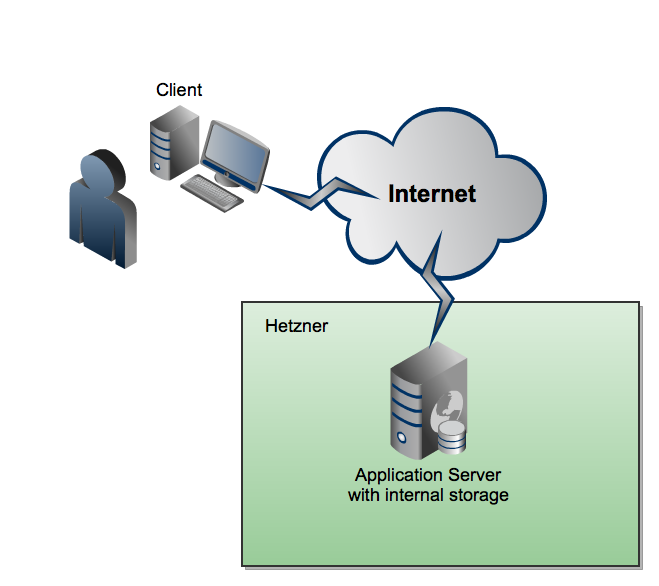
\includegraphics[width=\linewidth, keepaspectratio = true]{media/Hetzner.png}
\mycaption{figure}{\label{abb:Hetzner-Infrastruktur} Dezidierter Server System und Netzwerk Architektur }
\end{center}



\subsubsection*{Speicherkapazität}
Der grösste dedizierte Server, welcher Hetzner in seinem Produktkatalog führt, ist der Root-Server XS 29. Der XS 29 ist mit 15 mal 3 Terabyte SATA Festplatten ausgerüstet. Mit dem zusätzlich eingebauten Hardware-RAID-Controller lassen sich die 15 Festplatten zu einen RAID zusammenfügen.
Als CPU hat der Server einen Intel Xeon E3-1245 Quad-Core eingebaut und verfügt über 16 Gigabyte Hauptspeicher. 

Die max. Grösse einer Datei ist vom Dateisystem abhängig. ext3 oder "third extended filesystem" genannt, ist bei den meisten bekannten Linux Distributoren das standard Dateisystem. Die maximale Grösse einer Datei hängt von der verwendeten Blockgrösse ab. Nach eigenen Tests ist die standard Blockgrösse bei Debian, Ubuntu, Red Hat und Suse 4 Kibibyte gross. Bei einer Blockgrösse von 4 Kibibyte, kann eine Datei maximal 2 Tebibyte und das Dateisystem 16 Tebibyte gross sein. \cite{Card1993}

Die maximale Anzahl an Objekten hängt von der Grösse des Dateisystems ab. Bei einem 16 Tebibyte unterstützt die standard Konfiguration maximal 17'592'186'044'416 Objekte. 

\subsubsection*{Verfügbarkeit}
Die RAID-5 Konfiguration mit 15 Festplatten im RAID, bietet mit 38,192 Tebibyte gemäss \refeqlb{eqn:MaxSpeicherkapazitätHeztner} bei einfacher Redundanz die grösst mögliche Speicherkapazität. Wegen der möglicherweise langen Wiederherstellungs-Zeit (MTTR) dieser Konfiguration, ist man darauf angewiesen, dass der Ausfall vom eigenen Überwachungssystem erkannt und nach Benachrichtigung des Hetzner Support die defekte Festplatte rasch ausgetauscht wird. Die Festplatten selber sind während des Betriebs austauschbar, es ist somit kein Unterbruch des Betriebs erforderlich.

Der eingesetzte LSI RAID Kontrolle lässt auch die Konfiguration einer Hot-Spare Festplatte zu. Ein Host-Spare Festplatte ist ein leere ungenutzte Festplatte, die beim Ausfall einer Festplatte im RAID automatisch die defekte Festplatte ersetzt. 

Da es sich nur um ein Server System handelt, ist ein standortübergreifende Verfügbarkeit der Daten nicht möglich.


\begin{equation}
\mbox{Max Speicherkapazität} = (15 -1)* 2,728 \mathrm{\ TiB}= 38,192 \mathrm{\ TiB}
\label{eqn:MaxSpeicherkapazitätHeztner}
\end{equation}

\begin{equation}
\mbox{Max Speicherkapazität mit Hostspare} = (15 -1-1)* 2,728 \mathrm{\ TiB}= 35,464 \mathrm{\ TiB}
\label{eqn:MaxSpeicherkapazitätHeztnerHotspare}
\end{equation}

\subsubsection*{Datenzugriff}
Der Datenzugriff findet lokal über POSIX IO statt, dass heisst das die Web-Applikation auf dem selben Server betrieben wird. 

Der Lese- und Schreibzugriff ist auf den Server begrenzt. Theoretisch könnte der Speicher mit Protokollen wie NFS zwischen mehreren Systemen geteilt werden. Es handelt sich beim System um einen Miet-Server. Es kann deshalb nicht davon ausgegangen werden, dass weitere Miet-Server am selben Netzwerk-Knoten angeschlossen sind, oder sich sogar im gleichen Rechenzentrum befinden. Es muss aus diesen Gründen mit einer schlechten Bandbreite mit hoher Latenz zwischen den Systemen gerechnet werden, was die Teilung des Speichers aus Performancegründen unbefriedigend macht.

\begin{center}
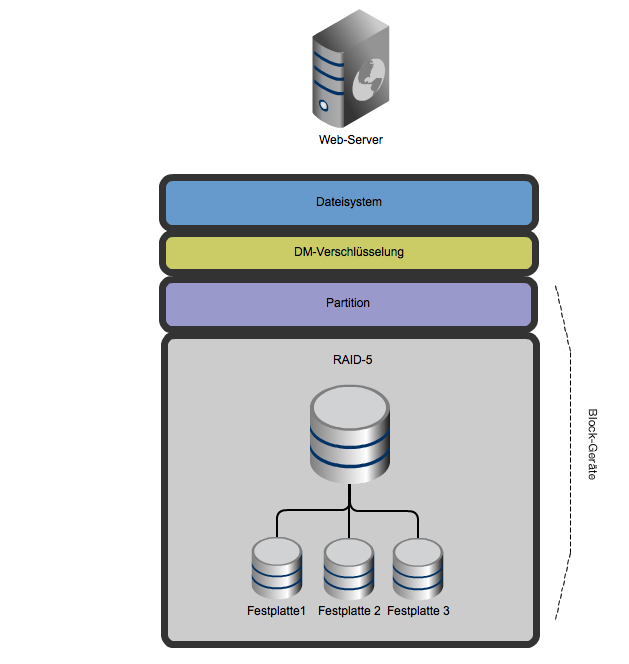
\includegraphics[width=\linewidth, keepaspectratio = true]{media/HetznerRAID.png}
\mycaption{figure}{\label{abb:HetznerRaidSpeicher} Interne Speicherarchitektur }
\end{center}

\subsubsection*{Datenschutz}
Die Integrität der Daten wird nur auf RAID Ebene sichergestellt und nicht auf Objekt-Ebene. Die Selbstheilung von Objekten wird nicht unterstützt.

Die Daten können mit einen RSYNC Job gesichert werden. Gegen eine zusätzliche Gebühre von 79 € für 10 GB ist die Datensicherung bei Hetzner möglich.

Der Datenzugriff lässt sich über die Dateiberechtigung im Dateisystem auf Benutzer- und Gruppen-Ebene steuern. Gegen den unerlaubten physischen Datenzugriff bietet die Verschlüsselung der Disk einen ausreichenden Schutz.

\subsubsection*{Technologie}
Die Konfiguration und Betrieb des Server inklusive RAID ist dem Mieter überlassen. Die RAID Technologie ist eine viel eingesetzte und bewährte Technologie.

Für die Konfiguration und den Betrieb des Servers reicht das Administratoren-Wissen für standard Linux aus.

Die Verwaltung des Speichers erfolgt über Kommandozeile bzw. über \gls{SSH}.

\subsubsection*{Kosten}
Abgesehen von den einmaligen Einrichtungskosten von 499 € und den Server Installationskosten gibt es keine weitere Investitionskosten. 

Für die Installation und Betrieb des gemieteten Servers ist der Mieter selber verantwortlich. Die Mietkosten betragen pro Monat 299 €.

Die Kosten für die Miete des Servers bleiben während der gesamten Mietdauer konstant. Die Kündigung ist jeweils auf 30 Tage zum Monatsende möglich. 

\paragraph*{Kosten Szenario-1}
Die Kosten für Szenario-1 betragen gemäss Zusammenstellung der Tabelle (10.9) Total € 11'163.00. Das entspricht zum aktuellen Tageskurs (13 April 2012) 13'422.95 CHF.

\begin{table}[htbp]
\caption{Kosten Hetzner S1}
\begin{small}
\begin{tabular}{|l|r|r|r|}
\hline
\textbf{Beschreibung} & \multicolumn{1}{l|}{\textbf{Kosten pro Stk/M.}} & \multicolumn{1}{l|}{\textbf{Anzahl}} & \multicolumn{1}{l|}{\textbf{Total}} \\ \hline
 \multicolumn{ 4}{c}{} \\ \hline
\multicolumn{ 4}{|c|}{\textbf{Investitionskosten}} \\ \hline
Einrichtung Root Server XS 29 & € 499.00 & 1 & € 499.00 \\ \hline \hline
 \multicolumn{ 3}{r|}{\textbf{Total:}} & \textbf{€ 499.00} \\ 
 \cline{4-4}
\multicolumn{ 4}{c}{} \\ \hline
\multicolumn{ 4}{|c|}{\textbf{Fortlaufende Kosten}} \\ \hline
Root Server XS 29 & € 299.00 & 1 & € 299.00 \\ \hline \hline
 \multicolumn{ 3}{r|}{\textbf{Total pro Monat:}} & € 299.00 \\
\cline{4-4}
 \multicolumn{ 3}{r|}{\textbf{Total 36 Monate:}} & \textbf{€ 10'764.00} \\ \cline{4-4}
 \multicolumn{ 4}{c}{} \\ \cline{4-4}
 \multicolumn{ 3}{r|}{\textbf{Total Gesamt:}} & \textbf{€ 11'163.00} \\ \cline{4-4}
\end{tabular}
\end{small}
\label{KostenHetznerS1}
\end{table}


\paragraph*{Kosten Szenario-2}
Es ist kein Produkt erhältlich, welches die Anforderungen der vorgeschlagenen Speicherkapazität von Szenario-2 erfüllen könnte.

\subsection{\ref{Al-2} und \ref{Al-3}: Netapp NFS und iSCSI}

Wie in der Markt Analyse erwähnt, ist NetApp der führende Anbieter im mittleren (engl. midrange) und oberen (Highend) Bereich von NAS und Speicherlösungen. Für beide Szenarien wurde das Modell FAS2240-4 gewählt. 

\subsubsection*{Verfügbarkeit}
Die Netapp hat mehrere Mechanismen für die Sicherstellung der Datenverfügbarkeit. So werden die Festplatten mittels RAID-DB System zusammen gefasst. RAID-DP ist eines auf Basis von RAID-4 von NetApp weiterentwickeltes RAID. Bei RAID-DP wird jedoch im Unterschied zu RAID-4 eine zusätzliche Paritäts-Festplatte eingesetzt. Wie in \refabb{abb:RAID-DP} ersichtlich, gibt es ein horizontale Parität und eine diagonale Parität. Die diagonale Parität ist durch die Farben dargestellt und auf der Festplatte DP gespeichert. Die horizontale Parität ist auf der Festplatte P gespeichert. Die mit D bezeichneten Festplatten sind normale RAID Daten-Festplatten. Die doppelte Parität hat den Vorteil, dass die Verfügbarkeit des RAID erhöht wird. So können bei einem RAID-DP gleichzeitig zwei Festplatten zur gleichen Zeit ausfallen, ohne dass dies zu einem Datenverlust führt, was in der Praxis immer wieder mal vorkommt. Im Vergleich dazu kann RAID-4 oder RAID-5 nur den Ausfall einer Festplatte kompensieren. \cite{White2010}

\begin{center}
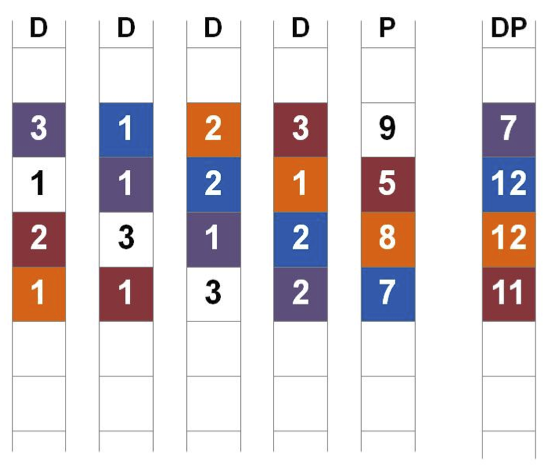
\includegraphics[ keepaspectratio = true]{media/raid-dp.png}
\mycaption{figure}{\label{abb:RAID-DP}NetApp RAID-DP doppelte Parität \cite{White2010}}
\end{center}

Als weitere Schutzmassnahme vor Datenverlusten empfiehlt NetApp den Einsatz von Spare-Festplatten. Durch den Einsatz von Spare-Festplatten kann die Wiederherstellungszeit MTTR verkleinert werden, da die Wiederherstellung automatisch starten kann. Die Anzahl an Spare-Festplatten ist abhängig von der Anzahl Festplatten und Enclosure.

Die NetApp FAS2240-4 ist mit zwei Storage Controller im Aktiv-/Aktiv-Betrieb mit Cluster Failover Funktion ausgerüstet.


\subsubsection*{Datenzugriff}
Der Datenzugriff auf die NetApp kann per NFS, CIFS, iSCSI oder Fibre Channel erfolgen.

Bei NFS ist es möglich, dass mehrere Server simultan eine Datei lesen. Das simultane Schreiben wird mit einem Sperr-Verfahren (engl. Locking) verhindert, damit die Dateikonsistenz gewährleistet bleibt.

Bei iSCSI wird der simultane Lesezugriff auf Dateien mittels clusterfähigem Dateisystem und Volume-Manager wie dem Global Filesystem bzw. LVM sichergestellt. Der simultane Schreibzugriff wird vom Dateisystem mit einem Sperrverfahren verhindert.

\subsubsection*{Speicherkapazität}
Die maximale Grösse einer Datei bzw. eines Objekts wird bei NetApp durch die maximale Grösse des Aggregates bestimmt. Seit der Betriebsystem-Version OnTab 8.0 sind Aggregate von 100 TiB möglich.

Bei iSCSI werden auf der NetApp LUN Dateien erstellt, die über iSCSI anderen Servern zur Verfügung gestellt werden. Die LUN Datei ist für den zugeteilten Server wie eine gewöhnliche Disk. Die Limitierungen für die maximale Dateigrösse und maximale Anzahl an Dateien wird bei iSCSI nicht mehr durch die NetApp limitiert, sondern durch das auf dem Server verwendete Dateisystem. So gewährleistet Red Hat für Global Filesystem (GFS) maximal ein 100 Terabyte grosses Dateisystem produktiv zu betreiben. Dieselbe Einschränkung gilt für Dateien. 

Die Anzahl möglicher Objekte, die in einen NetApp Volumen gespeichert werden können, werden durch die Anzahl Inodes des WAFEL Dateisystem bestimmt. NetApp legt standardmässig für jedes 32KiB eine Inode an. Bei einen 100 TiB Volume können somit maximal 3'355'443'200 Objekte gespeichert werden (\refeql{eqn:MaxObjekteNetApp}).

\begin{equation}
\mbox{Max Objekte} = \frac{107'374'182'400 \mathrm{\ KiB}}{32 \mathrm{\ KiB}}= 3'355'443'200 
\label{eqn:MaxObjekteNetApp}
\end{equation}

Die maximale Anzahl möglicher Objekte eines GFS Dateisystem ist variable. Inodes werden dynamisch alloziert.

\subsubsection*{Datenschutz}
NetApp speichert die Daten auf die Disk in 4 Kilo Byte Blocks. Zu jedem 4 Kilo Byte Block berechnet NetApp ein Prüfsumme und speichert diese in die Block Metadaten. Wenn der Block zu einem späteren Zeitpunkt wieder gelesen wird, berechnet die NetApp die Prüfsumme erneut und vergleicht diese mit der gespeicherten Prüfsumme. Stimmt diese nicht überein, wird der Block mittels den Paritäts-Daten neu geschrieben, erneut gelesen und geprüft. Um die Integrität von Daten zu gewährleisten, auf welche über einen längeren Zeitraum nicht mehr zugegriffen wurde, wie dies zum Beispiel bei Archivdaten der Fall ist, bietet NetApp ein konfigurierbare RAID Funktion (engl. RAID scrub) zum Durchkämmen und Prüfen der Daten. Die Funktion kann zeitgesteuert durchgeführt werden oder wenn das System sich im Leerlauf befindet. \cite{Sundaram2006}

Zu beachten ist, dass die Prüfsumme auf dem Block nur auf der Speicherebene Wirkung hat. Fehler die in einer höheren Ebene entstanden sind, wie zum Beispiel beim Einsatz von iSCSI zusammen mit einen Dateisystem, könnte bereits ein Fehler im Dateisystem durch einen Softwarefehler oder Memoryfehler entstanden sein. 

NetApp bietet mehrere Möglichkeiten eine Sicherungskopie der Daten herzustellen. Beim Einsatz von NFS oder iSCSI können die Daten über die Web-Servern mit einer handelsüblichen Sicherungs-Software gesichert werden. Bei NFS wird dazu die angefügten NFS Freigaben gesichert, bei iSCSI werden die Daten wie bei allen anderen Dateisystemen gesichert. Zu beachten ist bei diesen Verfahren, dass die Daten von der NetApp über den Server transferiert werden müssen und dadurch der Web-Server mit der Sicherungsaufgabe belastet wird. Neben der Sicherung der NetApp über den Server lässt sich die NetApp auch direkt sichern. Diese erfolgt mittels Network Data Management Protocol (NDMP) oder Mittels Snapshots. 

NDMP ist eines von NetApp mitentwickeltes Protokoll, welches für die Sicherung von NAS Geräte entwickelt wurde. Das Problem bei NAS Geräte ist, dass auf ihnen ein dediziertes Betriebsystem läuft, welche nicht erlaubt einen Sicherungs-Agenten zu installieren. Deswegen wurde das NDMP Protokoll entwickelt, um ein allgemeines agentenfreies Sicherungsverfahren für NAS Geräte zu ermöglichen. NDMP wurde dem IETF im Jahr 2000 von der NDMP Initianten als Entwurf eingereicht. Bis anhin ist jedoch noch kein RFC für NDMP standardisiert worden. Trotzdem wird es von vielen NAS-Geräte- und Sicherungs-Software- Herstellern unterstützt. Ein Liste mit Sicherungs-Software Produkten, welche das NDMP Verfahren unterstützen gibt es auf der Webseite der NDMP Initianden\footnote{\url{http://www.ndmp.org/products/index.shtml#backup}} zu finden. \cite{NDMP.orga}\cite{NDMP.org}

Beim Snapshots Sicherungsverfahren werden zeitbezogene Sicherungen des Dateisystem erstellt. Bei den Snapshots wird nicht eine eigentliche Kopie der Daten bzw. Blöcke erstellt, sondern die Referenz auf die Blöcke gespeichert. Wird nach dem Erstellen eines Snapshots ein Block geändert wird die Änderung nicht im Originalblock vorgenommen, sondern in einem neuen Block und diesen referenziert. Dadurch benötigt ein Snapshot einen minimalen Speicherplatz. Zudem lassen sich die Snapshots und damit die Sicherung in wenigen Sekunden erstellen, unabhängig von der Anzahl Dateien oder der verwendeten Speicherkapazität. Durch den Einsatz von zwei NetApp Systemen und der SnapMirror Funktion kann, das ganze Dateisystem bzw. Volume inklusive aller Snapshots auf der zweiten NetApp gesichert werden. Die Sicherung mit Snapshots hat bei grossen Datenmengen entscheidende Vorteile. Die Sicherung benötigt minimalen Speicherplatz, die Sicherung und Wiederherstellung ist innert Sekunden erstellt bzw. wiederhergestellt. Nachteile sind, dass der Speicherplatz mit der Sicherung bzw. Snapshots geteilt werden muss und das Löschen von Daten zusätzlichen Speicherplatz verbraucht.

Bei Bedarf kann die Kommunikation zwischen Speichersystem und Applikations-Server mit IPSec abhörsicher verschlüsselt werden. Zusätzlich bietet NetApp ab Version 8 die Verschlüsselung der ganzen Disk an.
%Sicherheit NFS IPSEC, intern

\subsubsection*{Technologie}
Die Firma NetApp beschäftigt in der Schweiz an ihren drei Standorten, Wallisellen, Lausanne und Bern ca. 80 Mitarbeiter. Zudem verfügt NetApp Schweiz über ein gut ausgebautes Partner Netzwerk, mit welchem die ganze Schweiz gut abgedeckt werden kann. Mit FastLane und QSkills sind zwei Schulungspartner im Raum Zürich verfügbar, welche offizielle Kurse und Zertifizierungen für NetApp Produkte anbieten. 

Neben den allgemeinen Garantie-Gewährleistungen bietet NetApp weitere kostenpflichtige Supportleistungen an. So steht eine Anlaufstelle mit dem SupportEdge Premium, den Remote Support mit einer Reaktionszeit von minimal 30 Minuten rund um die Uhr zur Verfügung. Die Installation von Ersatzteilen steht mit einer Reaktionszeit von minimal 2 Stunden rund um die Uhr zur Verfügung. 

Für den Support und Wartung stehen mehrere Produkte bereit, wie die Verlängerung der Hardware-Garantie, der Auto-Support mit oder ohne Austausch der Hardware durch NetApp.

Für die Verwaltung der NetApp stehen neben einer Kommandzeilen, Web-Interface und weitere teilweise kostenpflichtige Lösungen von NetApp zur Verfügung. 

\subsubsection*{Kosten}

\paragraph*{Kosten Szenario-1}
Die Kosten für Szenario-1 betragen gemäss Zusammenstellung total 225'711.15 CHF. Davon sind 44'811.15 CHF Investitionskosten und 180'900.00 CHF laufende Kosten für drei Jahre.

\begin{table}[htbp]
\caption{Kosten NetApp NFS/iSCSI Szenario-1}
\begin{small}
\begin{tabular}{|l|r|r|r|}
\hline
\textbf{Beschreibung} & \multicolumn{1}{l|}{\textbf{Kosten pro Stk/M.}} & \multicolumn{1}{l|}{\textbf{Anzahl}} & \multicolumn{1}{l|}{\textbf{Total}} \\ \hline
 \multicolumn{ 4}{c}{} \\ \hline
\multicolumn{ 4}{|c|}{\textbf{Investitionskosten}} \\ \hline
Dell PowerConnect 8024 & CHF 14'732.00 & 1 & CHF 14'732.00 \\ \hline
NetApp FAS2240-2 12*2TB & CHF 29'429.15 & 1 & CHF 29'429.15 \\ \hline
Rack Einrichtung & CHF 650.00 & 1 & CHF 650.00 \\ \hline \hline
 \multicolumn{ 3}{r|}{\textbf{Total:}} & \textbf{CHF 44'811.15} \\ 
 \cline{4-4}
\multicolumn{ 4}{c}{} \\ \hline
\multicolumn{ 4}{|c|}{\textbf{Fortlaufende Kosten}} \\ \hline
Dell Service & CHF 0.00 & 2 & CHF 0.00 \\ \hline
Rackkosten 11 U (500 W) & CHF 450.00 & 1 & CHF 450.00 \\ \hline
Strom 500 W & CHF 165.00 & 5 & CHF 825.00 \\ \hline
Personal & CHF 3'750.00 & 1 & CHF 3'750.00 \\ \hline \hline
 \multicolumn{ 3}{r|}{\textbf{Total pro Monat:}} & CHF 5'025.00 \\
\cline{4-4}
 \multicolumn{ 3}{r|}{\textbf{Total 36 Monate:}} & \textbf{CHF 180'900.00} \\ \cline{4-4}
 \multicolumn{ 4}{c}{} \\ \cline{4-4}
 \multicolumn{ 3}{r|}{\textbf{Total Gesamt:}} & \textbf{CHF 225'711.15} \\ \cline{4-4}
\end{tabular}
\end{small}
\label{KostenNetAppS1}
\end{table}


\paragraph*{Kosten Szenario-2}
Die Kosten für Szenario-1 betragen gemäss Zusammenstellung total 884'772.44 CHF. Davon sind 550'152.44 CHF Investitionskosten und 334'620.00 CHF laufende Kosten für drei Jahre.

% Zur Bereitstellung der 306 TiB sind 5 Disk Selfs des Typs DS4243 in der maximal Konfiguration mit 24 mal 3 TB SATA Festplatten erforderlich.

% Gemäss \refeqlb{eqn:AnzahlRackNetappS2} werden zwei ganze Racks für den Einbau aller Komponenten benötigt. Der benötigte Rackplatz entspricht dem Full Rack Angebot von Nine, welches 47 Rack-Höheneinheiten platz bietet. Der Preis pro Rack beträgt 1450 CHF pro Monat, plus 1500 CHF für die einmalige Einrichtung des Racks durch Nine.

% \begin{equation}
% \mbox{Anzahl Rack} = \frac{2*4\mathrm{\ U}+10*\mathrm{\ U}+2*1\mathrm{\ U}}{47\mathrm{\ U} } \approx 2 \mbox{(Auf ganze Rack gerundet)}
% \label{eqn:AnzahlRackNetappS2}
% \end{equation}
 

\begin{table}[htbp]
\caption{Kosten NetApp NFS/iSCSI Szenario-2}
\begin{small}
\begin{tabular}{|l|r|r|r|}
\hline
\textbf{Beschreibung} & \multicolumn{1}{l|}{\textbf{Kosten pro Stk/M.}} & \multicolumn{1}{l|}{\textbf{Anzahl}} & \multicolumn{1}{l|}{\textbf{Total}} \\ \hline
 \multicolumn{ 4}{c}{} \\ \hline
\multicolumn{ 4}{|c|}{\textbf{Investitionskosten}} \\ \hline
Dell PowerConnect 8024 & CHF 14'732.00 & 2 & CHF 29'464.00 \\ \hline
NetApp FAS2240-2 24*3TB & CHF 51'133.77 & 2 & CHF 102'267.54 \\ \hline
Disk Shelf DS4243 24*3TB & CHF 40'251.65 & 10 & CHF 402'516.50 \\ \hline
SnapMirror Lizenz & CHF 11'404.40 & 1 & CHF 11'404.40 \\ \hline
Rack Einrichtung & CHF 1'500.00 & 2 & CHF 3'000.00 \\ \hline 
Multi-Site Einrichtung & CHF 1'500.00 & 1 & CHF 1'500.00 \\ \hline \hline
 \multicolumn{ 3}{r|}{\textbf{Total:}} & \textbf{CHF 550'152.44} \\ 
 \cline{4-4}
\multicolumn{ 4}{c}{} \\ \hline
\multicolumn{ 4}{|c|}{\textbf{Fortlaufende Kosten}} \\ \hline
Dell Service & CHF 0.00 & 2 & CHF 0.00 \\ \hline
Rackkosten 47 U (2000 W) & CHF 1450.00 & 2 & CHF 2'900.00 \\ \hline
Strom 500 W & CHF 165.00 & 13 & CHF 2'145.00 \\ \hline
Mulit-Site 1 GBit/s & CHF 500.00 & 1 & CHF 500.00 \\ \hline
Personal & CHF 3'750.00 & 1 & CHF 3'750.00 \\ \hline \hline
 \multicolumn{ 3}{r|}{\textbf{Total pro Monat:}} & CHF 9'295.00 \\
\cline{4-4}
 \multicolumn{ 3}{r|}{\textbf{Total 36 Monate:}} & \textbf{CHF 334'620.00} \\ \cline{4-4}
 \multicolumn{ 4}{c}{} \\ \cline{4-4}
 \multicolumn{ 3}{r|}{\textbf{Total Gesamt:}} & \textbf{CHF 884'772.44} \\ \cline{4-4}
\end{tabular}
\end{small}
\label{KostenNetAppS2}
\end{table}

\subsection{\ref{Al-4}: OpenStack Objekt Storage}
OpenStack Object Storage ist ein quelloffene, frei verfügbare verteilte Speicherlösung. OpenStack Object Storage selbst ist kein Dateisystem, sondern eher ein Speicher-Cluster, welcher primär für die Speicherung von Virtual Maschine Images, Bilder, E-Mail und Sicherungskopien vorgesehen ist. Für einen OpenStack Cluster kommen vergleichbar mit dem Google Filesystem, kostengünstige konventionelle Computer-Hardware zum Einsatz. 

In \refabb{abb:OpenStack-Infrastruktur} zeigt die System und Netzwerk Architektur der OpenStack Object Storage Infrastruktur. Die Infrastruktur besteht aus zwei Proxy und Authentifizierungs-Servern, welche mit den 5 Daten-Nodes, in welcher jeder eine eigene Zone repräsentiert, über ein privates geswitches Netzwerk verbunden sind. Die Applikations-Server-Farm oder Web-Farm greift über das öffentliche Netzwerk über die Proxy-Server auf den Speicher zu. Die Infrastruktur ist jeweil für Szenario-2 über zwei Standorte verteilt, hier Site A und Site B.

\begin{center}
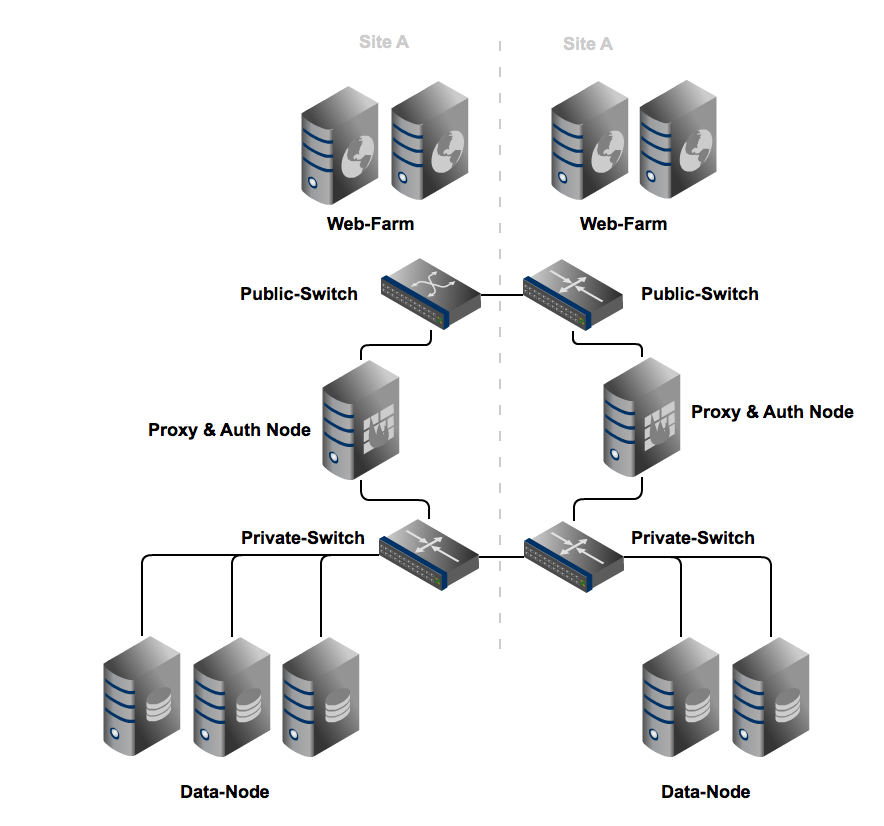
\includegraphics[width=\linewidth, keepaspectratio = true]{media/OpenStack.png}
\mycaption{figure}{\label{abb:OpenStack-Infrastruktur} OpenStack Infrastrutkur}
\end{center}


\subsubsection*{Verfügbarkeit}
OpenStack Object Storage wurde so konzipiert, dass ein Ausfall einer Hardwarekomponente den Weiterbetrieb aufrecht erhalten kann, ohne dabei einen Datenverlust oder die Verfügbarkeit des Systems zu gefährden. Die Daten bzw. Objekte werden redundant auf mehreren Zonen gespeichert. Zonen sind Gruppierungen von Servern. Die Anzahl redundanten Replikate für ein Objekt kann konfiguriert werden. Gewöhnlich werden drei Kopien verwaltet.

Für die Architektur wird von Joe Arnolds CEO bei SwiftStack bei dreifacher Redundanz die Implementierung von 5 Zonen empfohlen. OpenStack Object Storage, speichert die redundanten Objekte jeweils in einer separaten Zonen. Eine Zone kann bei kleinen Implementationen auch nur aus Gruppen von Festplatten bestehen, also innerhalb eines einzigen Servers existieren. Es wird aber empfohlen, eine Zone auf Hierarchie von Server-Gruppen zu implementieren. Das bedeutet, jede redundante Kopie ist auf einem eigenen Server gespeichert. \cite{Arnold} 

Zusätzlich zu den Speicherservern benötigt es noch zwei oder mehrere Proxy Server, um die hohe Verfügbarkeit zu gewährleisten. Die Proxy Server werden bei Rackspace mit 10 Gb Ethernet an den Netzwerk-Switch angeschlossen. \cite{OpenStack2011}

Möchte man den Speicher standortübergreifend betreiben, ist es erforderlich, dass pro Standort nicht mehr als $(Redundanz -1)$ Zonen betrieben werden, da ansonsten die Gefahr besteht, dass alle Replikate am gleichen Standort gespeichert werden. Das möchte niemand.

\subsubsection*{Speicherkapazität}
Der OpenStack Object Storage Cluster lässt sich im laufenden Betrieb ohne Unterbruch vergrössern. In der Regeln können auch Software Updates und Patches ohne Unterbruch des Clusters eingespielt werden, wenn darauf geachtet wird, nie mehr als eine Zone gleichzeitig zu aktualisieren.

Grundsätzlich ist die Anzahl an speicherbaren Objekten nicht begrenzt. Der Container Server von OpenStack Object Storage, dessen primäre Aufgabe es ist, die Auflistung der gespeicherten Objekten in einen Container zu verwalten, speichert die Informationen, welche Objekte sich im Container befinden. Pro Container in ein SQLite Datenbank angelegt. Die Performance der Datenbank, welche mit der Anzahl Einträge abnimmt, kann sich zum limitierenden Faktor entwickeln. Wie viele Objekte in einem Container gespeichert werden können. Der Performance Einbruch kann, je nach Leistung der Hardware und die generelle Last auf dem Cluster, bei ca. einer Million Objekten pro Container eintreten. Es können pro Account mehrere Container erstellt werden, wodurch die Limitierung entschärft wäre. Zu beachten ist hier, dass pro Account ebenfalls eine SQLite Datenbank mit allen Containern geführt wird und auch hier dieselben Einschränkungen zum tragen kommen. \cite{OpenStack2012}\cite{A2011}

\subsubsection*{Datenzugriff}
Der Zugriff auf die gespeicherten Objekten erfolgt ähnlich wie bei Amazon S3 über ein API. Das API verwendet für den Zugriff den standard HTTP Request. Verschiedene Speicherlösungs-Hersteller haben angekündigt, das Swift API ebenfalls für den Zugriff auf ihren Speicher unterstützen zu wollen. Glusterfs mit seiner verteilten Speicherlösung, bietet in der Entwicklerversion bereits die Unterstützung für Swift an. Applikationen, welche, das Swift API unterstützen, können ihre Speicherlösung künftig einfacher austauschen, ohne dabei die Applikation anpassen zu müssen. Neben dem Zugriff mit dem Swift API, bietet OpenStack eine Amazon S3 kompatibles API an. Der Zugriff über POSIX IO auf den Speicher ist nicht möglich.

Der Zugriff auf den Speicher erfolgt über einen Proxy, welcher den Speicherort des Objektes prüft und die Anfrage weiterleitet. Pro OpenStack Object Storage Cluster können mehrere Proxys eingesetzt werden. Mit Hilfe eines Load Balancers (Last Verteiler) können die Anfragen über die vorhandenen Proxys verteilt werden.

Die maximale Uploadgrösse beträgt 5 GB, die Downloadgrösse ist jedoch unbeschränkt. Wenn ein Objekt grösser als 5 GB hochgeladen wird, wird das Objekt in Teilen hochgeladen und gespeichert. Die Abfrage auf das Objekt erfolgt wie bei einem ganzen Objekt. Es müssen also keine Teile durch das API adressiert werden. \cite{OpenStack2012a}


\subsubsection*{Datenschutz}
OpenStack Object Storage stellt die Datenintegrität beim Speichern von Objekten und beim Auslesen der Daten sicher. Somit ist gewährleistet, dass die Daten im original gespeichert werden und bei der Speicherung kein Datenverlust entsteht. Die Selbstheilung von korrupten Objekten stellt OpenStack Objekt Storage mit dem Auditors Dien6st sicher. Der Auditors Dienst läuft auf jedem Server und prüft dort die Integrität von Objekten. Wenn ein korruptes Objekt erkannt wird, wird die Datei sofort unter Quarantäne gestellt und durch ein korrektes Reblikations-Objekt ersetzt.
Um die Last die durch den Auditors möglichst gering zu halten, kann die Anzahl Objekte oder die Anzahl Bits, die pro Sekunde geprüft werden, konfiguriert werden. \cite{OpenStack2012}

OpenStack Objekt Storage bietet neben der Redundanz der Objekte keine Möglichkeit, die Daten zu sichern. Dadurch ist keine Versionierung der Objekte möglich. Zwar lassen sich die Cluster Nodes mit einer konventionellen Sicherungssoftware direkt sichern. Dadurch lässt sich nur der gesamte Cluster wiederherstellen und nicht einzelne Objekte. Zudem wäre die Speicherkapazität pro Sicherung so gross wie es für die redundante Speicherung der Objekte Speicherkapazität benötigt würde. \cite{AndyBrezinsky2011}


Die Sicherheit der Daten wird mit sogenannten Accounts sichergestellt. Das heisst, dass ein Account nur auf seine gespeicherten Objekten zugreifen kann. Die Daten werden auf dem OpenStack Cluster unverschlüsselt in binärer Form gespeichert. Durch die Verteilung der Daten müsste jedoch ein Angreifer Zugriff auf alle Cluster Node erlangen, um an alle Daten eines Account zu gelangen.

\subsubsection*{Technologie}
OpenStack Objekt Storage wurde von der Firma RackSpace unter dem Code Name Swift entwickelt. Zusammen mit National Aeronautics and Space Administration (NASA) hat RackSpace die Softwareprojekt-Gemeinschaft OpenStack gegründet und Swift zusammen mit der Cloud-Lösung Nova für die Verwaltung von virtuellen Maschinen und Glace für die Verwaltung von Images als quelloffene Software veröffentlicht. Die OpenStack Gemeinschaft ist in Vergleich zu anderen quelloffenen Gemeinschaften noch eine relative jung Gemeinschaft. Es gelang ihr dennoch neben den beiden Gründerunternehmen weiter bedeutende Unternehmen aus der Informatikbranche, wie Hewlett Packard, Dell, Citrix, Intel, AMD, NetApp und weitere zu gewinnen. Eine vollständige Liste aller unterstützenden Unternehmen ist unter \url{http://openstack.org/community/companies/} zu finden. Die Aktivität auf der Projektseite von OpenStack Object Storage lässt erkennen, dass die Entwicklung aktiv vorangetrieben wird und viele Beiträge zu neuen Funktionen oder Verbesserungen von Anwendern und Entwickler beigetragen werden. \cite{Ohloh2012}

Die Internet-Recherche für auf OpenStack spezialisierte Schweizer Firmen ergaben keine Ergebnisse. 
Gemäss Internet-Recherchen gibt es noch keine spezialisierten Firmen für OpenStack Lösungen. Einige wenige Experten für OpenStack mit Domizil in der Schweiz konnten über die Profile bei LinkedIn, einem Social Network für Firmen, gefunden werden. 

Für die Verwaltung des Speichers bietet OpenStack ein Kommandozeilen-Tools an. Ein Web-GUI für Objekt Storage von OpenStack gibt es nicht. Die Firma SwiftStack bietet hierfür eine kostenpflichtige Lösung an. Die Überwachung des Speichers, zum Beispiel für die Verfügbarkeit einzelner Cluster Nodes, muss mit zusätzlichen Fremdlösungen erfolgen. 

\subsubsection*{Kosten}
Grundsätzlich unterscheiden sich die Kosten für die beiden Szenario nur in der Anzahl Server, den verwendeten Server Typen, der Anzahl Festplatten und dem benötigten Rackplatz. Die restlichen Faktoren sind für beide Szenarien gleich und werden in diesem Abschnitt behandelt.

Um die Rechenzentrumskosten möglichst tief zu halten, welche pro Rack verrechnet werden, soll möglichst viel Speicherkapazität in einer Rackeinheit gepackt werden. Dies bedeutet, dass die richtigen Server für die Anzahl der zur Verfügung gestellten Speicherkapazität verwendet werden sollen.

Um die Preise für die Festplatten möglichst tief zu halten werden diese separate beschaffen. Als Festplatte soll eine SATA-3 3.5 Zoll 3 Terabyte Festplatte eingesetzt werden. Dies entspricht 2.728 Tebibyte. Die Kosten für Festplatten sind stark marktabhängig, Für die Arbeit wird einfachheitshalber mit ca. 300 CHF pro Festplatte budgetiert.

Für beide Szenarien werden die gleichen Proxy-Server verwendet. Als Proxy Server wurden die Transtec Server-Systeme "'Lynx CALLEO Application Server 2260S'" ausgewählt. Die Proxy Server stammen vom selben Hersteller wie die in den Szenarien aufgeführten Datenserver. Dies hat den Vorteil, dass nur ein Ansprechpartner für die Server-Farm benötigt wird. Es ist kein Muss-Kriterium und kann bei Bedarf durch ein besseres Angebot eines anderen Herstellers ersetzt werden. Die Proxy sind mit einem Intel Xeon Prozessor E5-2665 mit 64 Gigabyte Hauptspeicher ausgerüstet. Die Server haben eine Rack-Höheneinheit von je 2 Einheiten. Wie bei den Datenserver wurde ein 365 mal 24 Stunden vor Ort Service ausgewählt. Der Preis pro Server beträgt 9'954 CHF.

Neben der Server Infrastruktur sind noch zwei Netzwerk-Switches notwendig. Der Dell PowerConnect 8024 bietet 24 Port mit 10GbE. Die Switches haben eine Rack-Höheneinheit von je 1 Einheiten und benötigen gemäss Hersteller maximal 237,77 Watt. Dell gewährt einen 3 Jahres Support für den Switch. Der Preis pro Switch beträgt 14'732 CHF.

Als Rechenzentrumsbetreiber wurde Nine Internet Solution ausgewählt. Nine betreibt ihr Rechenzentrum in Zürich und ist auf das Hosting spezialisiert. Mit seinem Rechenzentrumsstandort in der Stadt Zürich befindet sich Nine geographisch in der Nähe des Auftraggebers. Die Anfahrtszeit und der Anfahrtsweg kann so für den Auftraggeber kurz gehalten werden. Die verschiedenen Rack-Produkte, welche Nine anbietet, unterscheiden sich von der Anzahl Rack-Höheneinheiten und deren Watt-Leistung. In den Produkten ist zusätzlich die Anbindung ans Internet mit 100 Mbps enthalten. Bei zusätzlichem Wattbedarf bietet Nine die Möglichkeit, die zusätzliche Watts in 500er Pakete zu 165 CHF pro Monat an.

Für den den Betrieb der Speicherinfrastruktur wird mit einer Mannstelle gerechnet. Organisatorisch kann diese auch auf mehrere teilprozentuale Stellen aufgeteilt werden, damit auch der Betrieb während Ferienabwesenheiten sichergestellt ist. Pro Monat wird mit Personalkosten von 15'000 CHF gerechnet.


\paragraph*{Kosten Szenario-1}

Für die dreifache Redundanz sind für die aus der Soll-Analyse bestimmten 306 Tebibyte gemäss \refeqlb{eqn:SpeicherkapazitätS1} 918 Tebibyte an Speicherkapazität notwendig.

\begin{equation}
\mbox{Speicherkapazität}_{Redundanz} = 306 \mathrm{\ TiB} * 3 \mbox{\ Redundanz} = 918 \mathrm{\ TiB}
\label{eqn:SpeicherkapazitätS1}
\end{equation}


Als Server System wurde der Transtec Lynx CALLEO Application Server 1260 gewählt. Der Server basiert auf Server-Hardware des Herstellers SuperMicro. Der Server benötigt 1 Rack-Höcheneinheiten und bietet Platz für den Einbau von 4 3.5 Zoll Festplatten, welche auch während des Betriebs ausgetauscht werden können. Als Prozessoreinheit kommen ein Intel Xeon Prozessor E5-2620 zum Einsatz. Ferner verfügt der Server über 32 Gigabyte Hauptspeicher. Der Server wurde mit einem 3 Jahres, 24 Stunden, 365 Tage Vor-Ort Service gerechnet. Somit ist sichergestellt, dass im Störungsfall der Unterbruch möglichst gering gehalten werden kann. Der Preis pro Server beträgt ohne Festplatten 1'260 CHF.


Ein Server mit Festplatten ausgerüstet, weist gemäss der \refeqlb{eqn:SpeicherkapazitätServerS1} eine Speicherkapazität von 10,912 Tebibyte aus. Damit sind in anbetracht der notwendigen Speicherkapazität von 48,3 Tebibyte und der 5 Zonen insgesamt 5 Server notwendig (siehe \refeqlb{eqn:AnzahlServerS1}). Für die Speicherkapazität von 48,3 Tebibyte bei gleich ausgerüsteten Servern sind insgesamt nur 20 Festplatten notwendig.

\begin{equation}
\mbox{Speicherkapazität}_{Server} = 2,728 \mathrm{\ TiB} * 4 \mbox{\ Einschub} = 10,912 \mathrm{\ TiB}
\label{eqn:SpeicherkapazitätServerS1}
\end{equation}

\begin{equation}
\mbox{Anzahl Server} = \frac{48,3 \mathrm{\ TiB}}{10,912 \mathrm{\ TiB}} \approx 5 \mbox{\ (Auf 5 Zonen gerundet)}
\label{eqn:AnzahlServerS1}
\end{equation}

\begin{equation}
\mbox{Anzahl Festplatten} = \frac{48,3 \mathrm{\ TiB}}{2,728 \mathrm{\ TiB}} \approx 20 \mbox{\ (Auf 5 Server gerundet)}
\label{eqn:AnzahlServerS1}
\end{equation}

Gemäss \refeqlb{eqn:AnzahlRackS1} wird ein viertel-Rack für den Einbau aller Komponenten benötigt. Der Rackplatz entspricht dem Quarter Rack Angebot von Nine, welches 11 Rack-Höheneinheiten platz bietet. Der Preis pro Rack beträgt 450 CHF pro Monat, plus 650 CHF für die einmalige Einrichtung des Racks durch Nine.
Für die Berechnung der Gesamt Watt-Leistung fehlen die Angaben des Herstellers. Aus diesem Grund wird angenommen, dass der Daten-Server ca. 300 Watt und der Proxy-Server ca. 500 Watt bezieht. Mit diesen Annahmen benötigt es gemäss \refeqlb{eqn:AnzahlWattPaketeS1}, die 500 Watt, welche im Rackpreis enthalten sind, zusätzliche 5 Pakete a je 500 Watt pro Monat.

\begin{equation}
\mbox{Anzahl Racks} = \frac{5 * 1 \mathrm{\ U} + 2 * 2 \mathrm{\ U} + 2 * 2 \mathrm{\ U}}{11\mathrm{\ U}} \approx 1 \mbox{\ (Auf viertel Rack gerundet)}
\label{eqn:AnzahlRackS1}
\end{equation}

\begin{equation}
\mbox{Anzahl 500 \mathrm{W} Pakete} = \frac{5 * 300 \mathrm{\ W} + 2 * 500 \mathrm{\ W} +2 * 237,77 \mathrm{\ W} - 2000 \mathrm{\ W} }{500\mathrm{\ W}} \approx 5
\label{eqn:AnzahlWattPaketeS1}
\end{equation}

Wie aus der \reftab{tab:KostenOpenStackS1} ersichtlich ist, betragen die Gesamtkosten 653'646.50 CHF.


\begin{table}[htbp]
\caption{Kosten OpenStack S1}
\begin{small}
\begin{tabular}{|l|r|r|r|}
\hline
\textbf{Beschreibung} & \multicolumn{1}{l|}{\textbf{Kosten pro Stk/M.}} & \multicolumn{1}{l|}{\textbf{Anzahl}} & \multicolumn{1}{l|}{\textbf{Total}} \\ \hline
 \multicolumn{ 4}{c}{} \\ \hline
\multicolumn{ 4}{|c|}{\textbf{Investitionskosten}} \\ \hline
Dell PowerConnect 8024 & CHF 14'732.00 & 2 & CHF 29'464.00 \\ \hline
Lynx CALLEO App. Server 1260 & CHF 5'451.50 & 2 & CHF 10'903.00 \\ \hline
Lynx CALLEO App. Server 1260 & CHF 2'831.30 & 5 & CHF 14'156.50 \\ \hline
Festplatte 3,5 3 TB & CHF 300.00 & 20 & CHF 6'000.00 \\ \hline
Rack Einrichtung & CHF 650.00 & 1 & CHF 650.00 \\ \hline \hline
 \multicolumn{ 3}{r|}{\textbf{Total:}} & \textbf{CHF 61'173.50} \\ 
 \cline{4-4}
\multicolumn{ 4}{c}{} \\ \hline
\multicolumn{ 4}{|c|}{\textbf{Fortlaufende Kosten}} \\ \hline
Dell Service & CHF 0.00 & 2 & CHF 0.00 \\ \hline
Transtec Service (Server 1260) & CHF 26.08 & 2 & CHF 52.17 \\ \hline
Transtec Service (Server 1260) & CHF 26.08 & 5 & CHF 130.42 \\ \hline
Rackkosten 11 U (500 W) & CHF 450.00 & 1 & CHF 450.00 \\ \hline
Strom 500 W & CHF 165.00 & 5 & CHF 825.00 \\ \hline
Personal & CHF 15'000.00 & 1 & CHF 15'000.00 \\ \hline \hline
 \multicolumn{ 3}{r|}{\textbf{Total pro Monat:}} & CHF 16'457.58 \\
\cline{4-4}
 \multicolumn{ 3}{r|}{\textbf{Total 36 Monate:}} & \textbf{CHF 592'473.00} \\ \cline{4-4}
 \multicolumn{ 4}{c}{} \\ \cline{4-4}
 \multicolumn{ 3}{r|}{\textbf{Total Gesamt:}} & \textbf{CHF 653'646.50} \\ \cline{4-4}
\end{tabular}
\end{small}
\label{tab:KostenOpenStackS1}
\end{table}



\paragraph*{Kosten Szenario-2}

Für die dreifache Redundanz sind für die aus der Soll-Analyse bestimmten 306 Tebibyte gemäss \refeqlb{eqn:SpeicherkapazitätS2} 918 Tebibyte an Speicherkapazität notwendig.

\begin{equation}
\mbox{Speicherkapazität}_{Redundanz} = 306 \mathrm{\ TiB} * 3 \mbox{\ Redundanz} = 918 \mathrm{\ TiB}
\label{eqn:SpeicherkapazitätS2}
\end{equation}


Als Server-System wurde der Transtec Lynx CALLEO Application Server 4260 gewählt. Der Server basiert auf Server-Hardware des Herstellers SuperMicro, welche gemäss eigenen Recherchen auch bei anderen OpenStack Lösungen verwendet wird. Der Server benötigt 4 Rack-Höcheneinheiten Platz und bietet Platz für den Einbau von 36 3.5 Zoll Festplatten, welche auch während des Betriebs ausgetauscht werden können. Als Prozessoreinheit kommen zwei Intel Xeon Prozessor E5-2620 zum Einsatz. Ferner verfügt der Server über 64 Gigabyte Hauptspeicher. Der Server wurde mit einem 3 Jahres, 24 Stunden, 365 Tage Vor-Ort Service gerechnet. Somit ist sichergestellt, das im Störungsfall der Unterbruch möglichst gering gehalten werden kann. Der Preis pro Server beträgt ohne Festplatten 8'672 CHF.


Ein Server ausgerüstet mit Festplatten weist gemäss der \refeqlb{eqn:SpeicherkapazitätServerS2} eine Speicherkapazität von 98.208 Tebibyte aus. Damit sind in anbetracht der notwendigen Speicherkapazität von 918 Tebibyte und der 5 Zonen insgesamt 10 Server notwendig (siehe \refeqlb{eqn:AnzahlServerS2}). Für die Speicherkapazität von 918 Tebibyte bei gleich ausgerüsteten Servern sind insgesamt nur 340 Festplatten notwendig. Das heisst, pro Server sind 34 Einschübe mit Festplatten belegt. Sie könnten bei Bedarf noch weiter aufgerüstet werden.

\begin{equation}
\mbox{Speicherkapazität}_{Server} = 2,728 \mathrm{\ TiB} * 36 \mbox{\ Einschub} = 98.208 \mathrm{\ TiB}
\label{eqn:SpeicherkapazitätServerS2}
\end{equation}

\begin{equation}
\mbox{Anzahl Server} = \frac{918 \mathrm{\ TiB}}{98.208 \mathrm{\ TiB}} \approx 10 \mbox{\ (Auf 5 Zonen gerundet)}
\label{eqn:AnzahlServerS2}
\end{equation}

\begin{equation}
\mbox{Anzahl Festplatten} = \frac{918 \mathrm{\ TiB}}{2,728 \mathrm{\ TiB}} \approx 340 \mbox{\ (Auf 10 Server gerundet)}
\label{eqn:AnzahlServerS2}
\end{equation}

Gemäss \refeqlb{eqn:AnzahlRackS2} wird ein ganzes Rack für den Einbau aller Komponenten benötigt. Der Rackplatz entspricht den Full Rack Angebot von Nine, welches 47 Rack-Höheneinheiten platz bietet. Der Preis pro halbes Rack beträgt 750 CHF pro Monat, plus 850 CHF für die einmalige Einrichtung des Racks durch Nine.
Für die Berechnung der Gesamt Watt-Leistung fehlen die Angaben des Herstellers. Aus diesem Grund wird angenommen, dass der Daten-Server ca. 700 Watt und der Proxy-Server ca. 500 Watt bezieht. Mit diesen Annahmen benötigt es gemäss \refeqlb{eqn:AnzahlWattPaketeS2}, den 2000 Watt, welche im Rackpreis enthalten sind, zusätliche 13 Pakete zu je 500 Watt pro Monat.

\begin{equation}
\mbox{Anzahl Racks} = \frac{10 * 4 \mathrm{\ U} + 2 * 2 \mathrm{\ U} + 2 * 2 \mathrm{\ U}}{47\mathrm{\ U}} \approx 1 \mbox{\ (Auf ganze Rack gerundet)}
\label{eqn:AnzahlRackS2}
\end{equation}

\begin{equation}
\mbox{Anzahl 500 \mathrm{W} Pakete} = \frac{10 * 700 \mathrm{\ W} + 2 * 500 \mathrm{\ W} +2 * 237,77 \mathrm{\ W} - 2000 \mathrm{\ W} }{500\mathrm{\ W}} \approx 13
\label{eqn:AnzahlWattPaketeS2}
\end{equation}

Wie aus der \reftab{tab:KostenOpenStackS2} ersichtlich ist, betragen die Gesamtkosten 916'965.00 CHF.

\begin{table}[htbp]
\caption{Kosten OpenStack}
\begin{small}
\begin{tabular}{|l|r|r|r|}
\hline
\textbf{Beschreibung} & \multicolumn{1}{l|}{\textbf{Kosten pro Stk/M.}} & \multicolumn{1}{l|}{\textbf{Anzahl}} & \multicolumn{1}{l|}{\textbf{Total}} \\ \hline
 \multicolumn{ 4}{c}{} \\ \hline
\multicolumn{ 4}{|c|}{\textbf{Investitionskosten}} \\ \hline
Dell PowerConnect 8024 & CHF 14'732.00 & 2 & CHF 29'464.00 \\ \hline
Lynx CALLEO App. Server 1260 & CHF 5'451.50 & 2 & CHF 10'903.00 \\ \hline
Lynx CALLEO App. Server 4260H & CHF 6'111.00 & 10 & CHF 61'110.00 \\ \hline
Festplatte 3,5 3 TB & CHF 300.00 & 340 & CHF 102'000.00 \\ \hline
Rack Einrichtung & CHF 850.00 & 2 & CHF 1700.00 \\ \hline \hline
Mulit-Site Einrichtung & CHF 1500.00 & 1 & CHF 1500.00 \\ \hline \hline
 \multicolumn{ 3}{r|}{\textbf{Total:}} & \textbf{CHF 206'677.00} \\ \cline{4-4}
\multicolumn{ 4}{c}{} \\ \hline
\multicolumn{ 4}{|c|}{\textbf{Fortlaufende Kosten}} \\ \hline
Dell Service & CHF 0.00 & 2 & CHF 0.00 \\ \hline
Transtec Service (Server 1260) & CHF 26.08 & 2 & CHF 52.17 \\ \hline
Transtec Service (Server 4260H) & CHF 53.31 & 10 & CHF 533.06 \\ \hline
Rackkosten 22 U (1000 W) & CHF 750.00 & 2 & CHF 1'500.00 \\ \hline
Strom 500 W & CHF 165.00 & 13 & CHF 2'145.00 \\ \hline
Mulit-Site 1 GBit/s & CHF 500.00 & 1 & CHF 500.00 \\ \hline
Personal & CHF 15'000.00 & 1 & CHF 15'000.00 \\ \hline \hline
 \multicolumn{ 3}{r|}{\textbf{Total pro Monat:}} & CHF 19'730.22 \\ \cline{4-4}
 \multicolumn{ 3}{r|}{\textbf{Total 36 Monate:}} & \textbf{CHF 710'288.00} \\ \cline{4-4}
 \multicolumn{ 4}{c}{} \\ \cline{4-4}
 \multicolumn{ 3}{r|}{\textbf{Total Gesamt:}} & \textbf{CHF 916'965.00} \\ \cline{4-4}
\end{tabular}
\end{small}
\label{tab:KostenOpenStackS2}
\end{table}


\subsection{\ref{Al-5}: Amazon S3}
Amazon zählt zu den grössten, wenn nicht der grösste Online Speicheranbieter weltweit. Genaue Angaben über die Anzahl Kunden und Speicherkapazität veröffentlich Amazon nicht. Seit 2006 bietet Amazon Ihren Kunden unter dem Produktname S3, einen Online Speicher an. Die genaueren technischen Eigenschaften und Architektur des Online Speicher ist bis anhin von Amazon nicht veröffentlicht worden. Nach eigenen Angaben von Amazon basiert die Dienstleistung auf gewöhnlicher Computer Hardware.

Im \refabb{abb:AmazonS3-Infrastruktur} ist die Netzwerk und System-Architektur dargestellt. Es zeigt wie die Applikations-Server Farm Bildobjekte über das Internet auf dem Amazon S3 Speicher ablegt und darauf zugreift. Zudem zeigt die Abbildung wie eine Client-Anfrage auf ein Bildobjekt an die Applikations-Server Farm, den direkten URL Pfad zum Bildobjekt auf den Amazon S3 Speicher verweist. Somit kann die Auslieferung der Bilddaten direkt über Amazon S3 erfolgen, was die Bandbreite der Applikations-Server Farm entlastet. 

\begin{center}
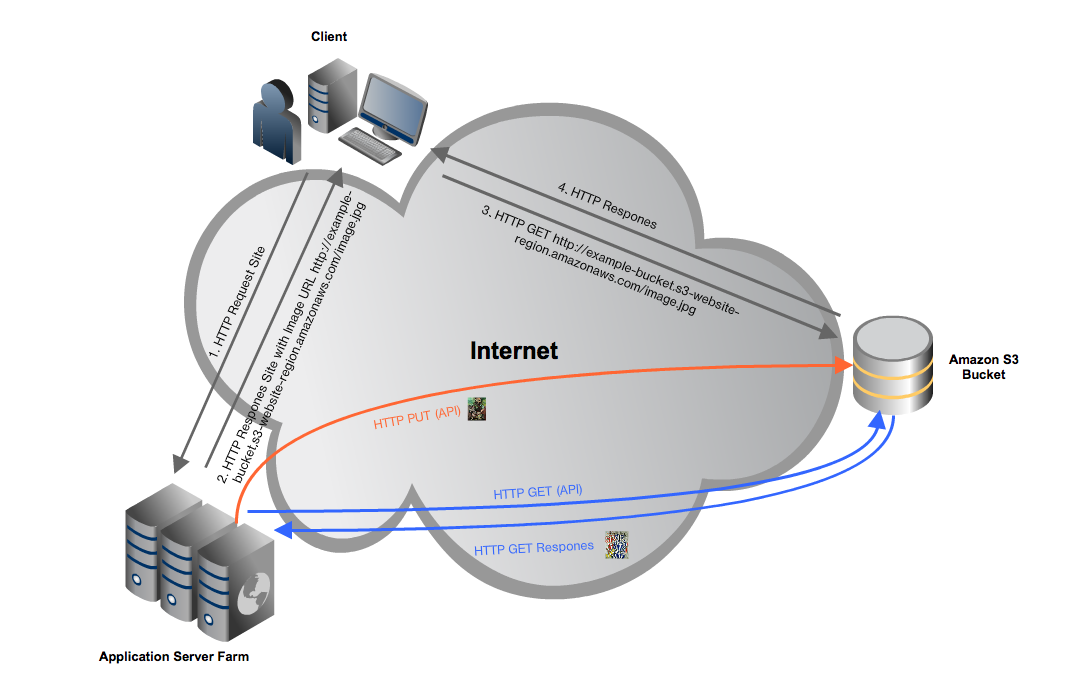
\includegraphics[width=\linewidth, keepaspectratio = true]{media/Amazon_S3.png}
\mycaption{figure}{\label{abb:AmazonS3-Infrastruktur} Amazon S3 Netz und System Architektur}
\end{center}




Bei Online Speicher wie Amazon S3, kann der Kunde gleich nach Anmeldung an den Dienst, die Speicherressourcen verwenden. Es fallen also keine Installationkosten für die Speicherinfrastruktur an. 

\subsubsection*{Verfügbarkeit}
Amazon S3 speichert die Daten auf mehreren Geräten in verschiedenen Rechenzentren in derselben Region ab. Beim Speichern werden die Daten synchron in verschiedene Rechenzentren abgelegt bevor die Speicherung als erfolgreich gemeldet wird. Damit ist sichergestellt, dass die Daten von Beginn weg einwandfrei redundant gespeichert sind. Mit diesen Massnahmen gewährleistet Amazon gemäss Dienstgütevereinbarung eine Zuverlässigkeit von 99.999999999\%. Bei Bedarf kann die Zuverlässigkeit für Daten, welche wenig Schutz benötigen, wie zum Beispiel Thumbnails von Bilder, mit einer geringeren Zuverlässigkeit von 99.99\% zu einem günstigeren Preis gespeichert werden. \cite{Amazon2007}

Durch die redundante Speicherung der Daten auf mehrere Geräte gewährleistet Amazone gemäss Dienstgütevereinbarung von 99.99\% pro Monat.

\subsubsection*{Datenzugriff}
Der Zugriff auf die Daten findet über eine API oder über die Verwaltungskonsole von Amazon statt. Für den Zugriff mit einem API bietet Amazon ein \gls{REST} und eine \gls{SOAP} Schnittstelle an. Der \gls{REST} Zugriff findet über HTTP statt. Dabei werden standard HTTP requests verwendet. Für den Zugriff kann auch ein gewöhnlicher Web-Browser verwendet werden solange die Objekte öffentlich sind.

Einen offiziellen POSIX IO Zugriff von Amazon steht nicht zur Verfügung. Es existiert allerdings ein quelloffenes Projekt Namens s3fs\footnote{\url{https://code.google.com/p/s3fs/}}, welches es ermöglicht, einen Amazon S3 Speicher unter Linux zu mounten. \cite{S3fs}

Da die Infrastruktur von Amazon S3 nicht bekannt ist, können keine detaillierten Angaben über die Skalierung der Datenzugriffe gemacht werden. Es kann von einem hochskalierbaren System ausgegangen werden, da Amazon die Zugriffe von tausenden von Kunden gleichzeitig handhaben muss.

Amazon S3 unterstützt das Lesen und Schreiben von mehreren Systemen. Beim Lesen einen Objektes, welches aus mehreren Systemen zugegriffen und beschrieben wird, stellt Amazon S3 die Lesekonsistenz sicher. \cite{Amazon2012a}

Für das Einlesen von grossen Datenmengen bietet Amazon einen kostenpflichtigen Import/Export Dienstleistung an. Bei dieser Dienstleistung sendet der Kunde die Daten gespeichert auf einem tragbaren Speichermedium an Amazon, welches die Daten direkt in ihre Cloud ohne Umwege über das Internet einliesst.

Die API von Amazon ist gut dokumentiert, weshalb für einen erfahrenen Entwickler die Anbindung der Web-Applikation an Amazon S3 umsetzbar sein sollte.

\subsubsection*{Speicherkapazität}
Für die Skalierung der Speicherkapazität kümmert sich Amazon.

Im Amazon S3 können eine unbegrenzte Anzahl von Objekten gespeichert werden, welche eine Speichergrösse von 1 Byte bis zu 5 Terrabyte haben können. In einem PUT können maximal 5 Gigabyte hochgeladen werden. Für das Hochladen von grösseren Objekten muss die Multipart Funktion verwendet werden, welche das Objekte in mehrere Teilen gliedert und hochladet. \cite{Amazon2012b}

\subsubsection*{Datenschutz}
Die Daten können bei Amazon in mehren Regionen gespeichert werden. Zu den verfügbaren Regionen gehören, US Standard, US West (Oregon), US West (Northern California), EU (Ireland), Asia Pacific (Singapore), Asia Pacific (Tokyo), South America (Sao Paulo). Gemäss Amazon verlassen die gespeicherten Daten eine Region nicht, ausser für die Erfüllung von Gesetzen oder auf Anforderung einer Regierung. Als US amerikanisches Unternehmen steht Amazon wegen dem Patriot Act unter der Pflicht, den US-Behörden auf Anforderung Zugang zu den Daten zu gewährleisten, auch wenn diese Informationen ausserhalb der USA gespeichert sind. Gemäss EU Recht dürfen ohne Einverständnis der Behörden keine gespeicherten Informationen an Dritten zugänglich gemacht werden, auch nicht solche Daten die ausserhalb der EU gespeichert sind. Bei Microsoft, ebenfalls ein grosser Cloud-Anbieter bestätigt diese Regel, dass die Daten nicht vor dem Zugriff der USA geschützt sind. \cite{Amazon2012}\cite{Ostler}

Die Integrität der Daten wird mit einer Prüfsumme sichergestellt. Die gespeicherten Daten werden von Amazon regelmässig auf ihre Integrität geprüft und bei Bedarf von einer integren Kopie der Daten ersetzt. 

Die Daten können verschlüsselt per SSL zugegriffen bzw. gespeichert werden. Somit ist gewährleistet, dass Dritte die Daten beim Transport nicht lesen können. Seit 2011 bietet Amazon kostenlos ebenfalls die Verschlüsselung mit AES-256 von Objekten im Speicher an. Dabei wird jedes Objekt mit einem eigenen Schlüssel ver- und entschlüsselt. Die erzeugten Schlüssel werden mit einem Master-Schlüssel ebenfalls verschlüsselt und auf den Amazon-Servern gespeichert. Das Schlüsselmanagment bleibt jedoch bei Amazon, weshalb man abhängig von den Massnahmen zum Schutz des Schlusselmanagment ist die Amazon alleine trifft. Wird diese kompromitiert oder fällt sie aus, ist der Zugriff auf die verschlüsselten Daten nicht mehr möglich. \cite{RobertLippert2011}

Die Berechtigung auf gespeicherte Objekte oder Ordner können mit einem Rechte-Management verwaltet werden. Objekte können öffentlich zugänglich gemacht werden oder nur an bestimmte authentifizierte Benutzer zur Verfügung gestellt werden. Zudem lassen sich Zugriffe auf Objekte protokollieren. \cite{Amazon2012b}

Für die Berechtigung und Verwaltung stellt Amazon ein Web-GUI zur Verfügung. Bis auf das Eröffnen eines Speichers und die Initialberechtigung sollten voraussichtlich nicht weitere Verwaltungsaufgaben anfallen.

Amazon bietet neben der Redundanz der Objekte kein weiteres Sicherungsverfahren an. Beim Herunterladen der Daten fallen für den Transfer zusätzliche Kosten an.

\subsubsection*{Technologie}
Der Online Speicher von Amazon S3 gilt als ausgereiftes und etabliertes Produkt im Markt. Es kann davon ausgegangen werden, dass die Dienstleistung über die nächsten vier Jahre hinaus bestehen wird und für den Kunden keine Migration notwendig ist. Amazon S3 wird ebenfalls von SmugMug, ein Photodienstleister, verwendet oder andere bekannte Web-Applikationen wie Dropbox verwendet. \cite{SmugMug}\cite{Dropbox2011}

Der Online-Speicher-Markt ist im Verhältnis zu anderen Speichermärkten noch relativ jung. Analysten wie Jeff Boles gehen davon aus, dass der Online-Speicher-Markt in den nächsten Jahren stark wachsen wird. Wie in der Marktstudie beschrieben, konnte Amazon seit dem Start des Amazon S3 Produktes die Anzahl gespeicherte Objekte jeweils pro Jahr mehr als verdoppeln (sie dazu \refabb{abb:AnzahlObjekteAmazonS3}). Die Konkurrenz wie Google, Microsoft oder Rackspace machen Amazon den Markt streitig. Der Kunden darf hoffen, dass die Anbieter ihre Preise noch spitzer kalkulieren müssen, um konkurrenzfähig zu bleiben. Amazon hat die Preise für S3 Speicher erst kürzlich angepasst. \cite{Boles2011}\cite{Barr2012a}


\subsubsection*{Kosten}
Durch den Bezug der Speicherressourcen als Dienstleistung fallen für den Kunden keine Investitionskosten für die Speicherinfrastruktur an.
Dafür muss in den meisten Fällen die Applikation für den Zugriff mittels Amazon S3 API programmiert werden, wodurch Entwicklungskosten anfallen können.

Beim Amazon S3 wird jeweils nur der effektiv verwendete Speicherplatz pro Monat verrechnet. Im Preis von Amazon ist jeweils die dreifache Redundanz inbegriffen. Der Speicherplatz kostet ab 1 Terabyte bis 49 Terabyte \$ 0.110 per Gigabyte. Ab 49 Terabyte bis 450 Terabyte reduzieren sich die Kosten pro Gigabyte auf \$ 0.095. Anders als beim Betrieb einer eigenen Speicherinfrastruktur muss der Kunden keine zusätzliche Speicherkapazitätsreserven für Unvorhergesehenes einrechnen, da diese erst bei Bedarf von Amazon zur Verfügung gestellt wird. Dies spart substantiell Kosten für den Kunden.

Bei Verwendung von Amazon S3 fallen für den Kunden zudem keine Wartungskosten für den Betrieb der Speicherinfrastruktur an. 

Im Vergleich zum eigenen Betrieb fallen dem Kunden allerdings Kosten für den Transfer und Abfragen der Daten an. So kostet der Transfer der Daten aus dem Amazon S3 Speicher für jedes GB \$ 0.12 bei einem Transfervolumen bis zu 10 TB. Für die Abfrage wird unterschieden zwischen schreibenden und lesenden Abfragen. Der Lesezugriff kostet pro 10'000 Abfragen \$ 0.01 und für jeden Schreibzugriff pro 1'000 Abfragen \$ 0.01. Die tatsächlichen Kosten sind schwierig vorherzusagen und könnten zu Überraschungen führen. Die zu budgetierenden Kosten sind stark von den Anzahl Benutzern und deren Benutzerverhalten abhängig und können saisonalen Schwankungen unterliegen.

\paragraph*{Kosten Szenario-1}
Die Kosten für Szenario-1 betragen gemäss Zusammenstellung der\reftab{tab:KostenAmazonS3S1} total \$ 42'646.32. Das entspricht zum aktuellen Tageskurs gerechnet (13 April 2012) 39'10.52 CHF. 


\subsubsection**{Kosten Szenario-2}
Die Kosten für Szenario-1 betragen gemäss Zusammenstellung der \reftab{tab:KostenAmazonS3S2} total \$ 493'902.84. Das entspricht zum aktuellen Tageskurs gerechnet (13 April 2012) 450'637.17 CHF. 

\begin{table}
\caption{Kosten Amazon S3 Szenario-1}
\begin{center}
\begin{tabular}{|l|r|r|r|}
\hline
\multicolumn{1}{|l|}{\textbf{Bezeichnung}} &\multicolumn{1}{|l|}{\textbf{Monat}} & \multicolumn{1}{l|}
{\textbf{Speicherkapazität}} & \multicolumn{1}{l|}{\textbf{Kosten}} \\ \hline
\multicolumn{4}{c}{} \\ \hline
\multicolumn{ 4}{|c|}{\textit{Investitionskosten}} \\ \hline 
- & & & \\ \hline
\multicolumn{3}{r|}{\textbf{Total:}} & CHF 0.00 \\ \cline{4-4}
\multicolumn{4}{c}{} \\ \hline
\multicolumn{ 4}{|c|}{\textit{Fortlaufende Kosten}} \\ \hline
Amazon S3 & 1 & 2,75 & \$691.82 \\ \hline
Amazon S3 & 2 & 3 & \$719.98 \\ \hline
Amazon S3 & 3 & 3,25 & \$748.14 \\ \hline
Amazon S3 & 4 & 3,5 & \$776.30 \\ \hline
Amazon S3 & 5 & 3,75 & \$804.46 \\ \hline
Amazon S3 & 6 & 4 & \$832.62 \\ \hline
Amazon S3 & 7 & 4,25 & \$860.78 \\ \hline
Amazon S3 & 8 & 4,5 & \$888.94 \\ \hline
Amazon S3 & 9 & 4,75 & \$917.10 \\ \hline
Amazon S3 & 10 & 5 & \$945.26 \\ \hline
Amazon S3 & 11 & 5,25 & \$973.42 \\ \hline
Amazon S3 & 12 & 5,5 & \$1'001.58 \\ \hline
Amazon S3 & 13 & 5,75 & \$1'029.74 \\ \hline
Amazon S3 & 14 & 6 & \$1'057.90 \\ \hline
Amazon S3 & 15 & 6,25 & \$1'086.06 \\ \hline
Amazon S3 & 16 & 6,5 & \$1'114.22 \\ \hline
Amazon S3 & 17 & 6,75 & \$1'142.38 \\ \hline
Amazon S3 & 18 & 7 & \$1'170.54 \\ \hline
Amazon S3 & 19 & 7,25 & \$1'198.70 \\ \hline
Amazon S3 & 20 & 7,5 & \$1'226.86 \\ \hline
Amazon S3 & 21 & 7,75 & \$1'255.02 \\ \hline
Amazon S3 & 22 & 8 & \$1'283.18 \\ \hline
Amazon S3 & 23 & 8,25 & \$1'311.34 \\ \hline
Amazon S3 & 24 & 8,5 & \$1'339.50 \\ \hline
Amazon S3 & 25 & 8,75 & \$1'367.66 \\ \hline
Amazon S3 & 26 & 9 & \$1'395.82 \\ \hline
Amazon S3 & 27 & 9,25 & \$1'423.98 \\ \hline
Amazon S3 & 28 & 9,5 & \$1'452.14 \\ \hline
Amazon S3 & 29 & 9,75 & \$1'480.30 \\ \hline
Amazon S3 & 30 & 10 & \$1'508.46 \\ \hline
Amazon S3 & 31 & 10,25 & \$1'536.62 \\ \hline
Amazon S3 & 32 & 10,5 & \$1'564.78 \\ \hline
Amazon S3 & 33 & 10,75 & \$1'592.94 \\ \hline
Amazon S3 & 34 & 11 & \$1'621.10 \\ \hline
Amazon S3 & 35 & 11,25 & \$1'649.26 \\ \hline
Amazon S3 & 36 & 11,5 & \$1'677.42 \\ \hline
\multicolumn{3}{r|}{\textbf{Total:}} & \textbf{\$ 42'646.32} \\ \cline{4-4}
\multicolumn{4}{c}{} \\ \cline{4-4}
\multicolumn{3}{r|}{\textbf{Total Gesamt:}} & \textbf{ \$ 42'646.32} \\ \cline{4-4}
\end{tabular}
\end{center}
\label{tab:KostenAmazonS3S1}
\end{table}

\begin{table}
\caption{Kosten Amazon S3 Szenario-2}
\begin{center}
\begin{tabular}{|l|r|r|r|}
\hline
\multicolumn{1}{|l|}{\textbf{Bezeichnung}} &\multicolumn{1}{|l|}{\textbf{Monat}} & \multicolumn{1}{l|}
{\textbf{Speicherkapazität}} & \multicolumn{1}{l|}{\textbf{Kosten}} \\ \hline
\multicolumn{4}{c}{} \\ \hline
\multicolumn{ 4}{|c|}{\textit{Investitionskosten}} \\ \hline 
- & & & \\ \hline
\multicolumn{3}{r|}{\textbf{Total:}} & CHF 0.00 \\ \cline{4-4}
\multicolumn{4}{c}{} \\ \hline
\multicolumn{ 4}{|c|}{\textit{Fortlaufende Kosten}} \\ \hline
Amazon S3 & 1 & 8.5 & \$2'937.87 \\ \hline
Amazon S3 & 2 & 14.5 & \$3'613.71 \\ \hline
Amazon S3 & 3 & 20.5 & \$4'289.55 \\ \hline
Amazon S3 & 4 & 26.5 & \$4'965.39 \\ \hline
Amazon S3 & 5 & 32.5 & \$5'641.23 \\ \hline
Amazon S3 & 6 & 38.5 & \$6'317.07 \\ \hline
Amazon S3 & 7 & 44.5 & \$6'992.91 \\ \hline
Amazon S3 & 8 & 50.5 & \$7'661.07 \\ \hline
Amazon S3 & 9 & 56.5 & \$8'244.75 \\ \hline
Amazon S3 & 10 & 62.5 & \$8'828.43 \\ \hline
Amazon S3 & 11 & 68.5 & \$9'412.11 \\ \hline
Amazon S3 & 12 & 74.5 & \$9'995.79 \\ \hline
Amazon S3 & 13 & 80.5 & \$10'579.47 \\ \hline
Amazon S3 & 14 & 86.5 & \$11'163.15 \\ \hline
Amazon S3 & 15 & 92.5 & \$11'746.83 \\ \hline
Amazon S3 & 16 & 98.5 & \$12'330.51 \\ \hline
Amazon S3 & 17 & 104.5 & \$12'914.19 \\ \hline
Amazon S3 & 18 & 110.5 & \$13'497.87 \\ \hline
Amazon S3 & 19 & 116.5 & \$14'081.55 \\ \hline
Amazon S3 & 20 & 122.5 & \$14'665.23 \\ \hline
Amazon S3 & 21 & 128.5 & \$15'248.91 \\ \hline
Amazon S3 & 22 & 134.5 & \$15'832.59 \\ \hline
Amazon S3 & 23 & 140.5 & \$16'416.27 \\ \hline
Amazon S3 & 24 & 146.5 & \$16'999.95 \\ \hline
Amazon S3 & 25 & 152.5 & \$17'583.63 \\ \hline
Amazon S3 & 26 & 158.5 & \$18'167.31 \\ \hline
Amazon S3 & 27 & 164.5 & \$18'750.99 \\ \hline
Amazon S3 & 28 & 170.5 & \$19'334.67 \\ \hline
Amazon S3 & 29 & 176.5 & \$19'918.35 \\ \hline
Amazon S3 & 30 & 182.5 & \$20'502.03 \\ \hline
Amazon S3 & 31 & 188.5 & \$21'085.71 \\ \hline
Amazon S3 & 32 & 194.5 & \$21'669.39 \\ \hline
Amazon S3 & 33 & 200.5 & \$22'253.07 \\ \hline
Amazon S3 & 34 & 206.5 & \$22'836.75 \\ \hline
Amazon S3 & 35 & 212.5 & \$23'420.43 \\ \hline
Amazon S3 & 36 & 218.5 & \$24'004.11 \\ \hline
\multicolumn{3}{r|}{\textbf{Total:}} & \textbf{\$ 493'902.84}
 \\ \cline{4-4}
\multicolumn{4}{c}{} \\ \cline{4-4}
\multicolumn{3}{r|}{\textbf{Total Gesamt:}} & \textbf{\$ 493'902.84}
 \\ \cline{4-4}
\end{tabular}
\end{center}
\label{tab:KostenAmazonS3S2}
\end{table}




\section{Evaluation KO Kriteren}
\subsection{Evaluation KO Kriteren Szenario-1}

\paragraph*{Untersuchung auf KO Kriterium \ref{KO-1}}
Alle Alternativen für das Szenario-1 unterstützen die Speicherung von Dateien bis 2 Gibibyte Speichergrösse (\refbf{KO-1}).

\paragraph*{Untersuchung auf KO Kriterium \ref{KO-2}}
Alle Alternativen aus dem Szenario-1 erfüllen die geforderten Speicherkapazität des Szenario-1.

\paragraph*{Untersuchung auf KO Kriterium \ref{KO-3}}
Die günstigste Lösung ist die Alternative \ref{Al-1} mit Gesamtkosten von 13'422.95 CHF. Gemäss KO Kriterium \ref{KO-3} dürfen die Kosten 40'268.85 CHF nicht überschritten werden. Mit Ausnahme von \ref{Al-5} mit Kosten von insgesamt 39'10.52 CHF überschreiten die Alternativen \ref{Al-2} (240’443.15 CHF), \ref{Al-3} (240’443.15 CHF) und \ref{Al-4} (653’646.50 CHF) die Kosten und werden somit von der weiteren Evaluation für das Szenario-1 ausgeschlossen.

\subsection{Evaluation KO Kriteren Szenario-2}

\paragraph*{Untersuchung auf KO Kriterium \ref{KO-1}}
Alle Alternativen für das Szenario-2 unterstützen die Speicherung von Dateien bis 2 Gibibyte Speichergrösse (\refbf{KO-1}).

\paragraph*{Untersuchung auf KO Kriterium \ref{KO-2}}
Bis auf Alternative \ref{Al-1}, welches kein Produkte für die geforderten Speicherkapazität hat, erfüllen alle die vorgegebene Speicherkapazität des Szenario-2. Die Alternative \ref{Al-1} wird somit für die weitere Evaluation für das Szenario-2 ausgeschlossen.

\paragraph*{Untersuchung auf KO Kriterium \ref{KO-3}}
Die günstigste Lösung ist die Alternative \refsoll{Al-5} \ref{Al-5} mit Gesamtkosten von 450'637.17 CHF. Gemäss KO Kriterium \ref{KO-3} dürfen die Kosten von 1'351'911.15 CHF nicht überschritten werden. Die Alternative \ref{Al-2} (884’772.44 CHF), \ref{Al-3} (884’772.44 CHF) und \ref{Al-4} (916’965.00) überschreiten die maximalen Kosten nicht. Die Alternative \ref{Al-1} bietet keine Produkt für Szenario-2.

\section{Evaluation Soll Kriteren}
Die Evaluation der Soll Kriterien und die dazugehörigen Begründungen für die Bewertung sind detailliert im Anhang aufgeführt. Die Bewertungen der Vergleiche der Alternativen wurden in das Programm AHP Decision eingegeben und ausgewertet.

\subsection{Auswertung Szenario-1}

Wie in \reftab{EvalResultS1} zu entnehmen ist, gewinnt die Alternative \refsoll{Al-5} \ref{Al-5} mit 0.698 Punkte oder 69.8\% die Evaluation von Szenario-1. Die Alternative \refsoll{Al-1} \ref{Al-1} hat insgesamt 0.302 Punkte oder 30.2 \% erreicht.

\begin{table}[htbp]
\caption{Evalutation Resultat Szenario-1}
\begin{center}
\begin{tabular}{|c|l|r|}
\hline
Rang & Alternativen & \multicolumn{1}{l|}{Priorität} \\ \hline
1 & Amazon S3 & 0.698 \\ \hline
2 & Hetzner & 0.302 \\ \hline
\end{tabular}
\end{center}
\label{EvalResultS1}
\end{table}


\subsection{Auswertung Szenario-2}

Wie in \reftab{EvalResultS2} zu entnehmen ist, gewinnt die Alternative \refsoll{Al-5} \ref{Al-5} mit 0.310 Punkte oder 31\% die Evaluation. Auf dem zweiten Platz folgt \refsoll{Al-3} \ref{Al-3} mit 0.236 Punkte oder 23.6\%, dicht gefolgt vom drittklassierten \refsoll{Al-4} \ref{Al-4} mit 0.36 Punkte oder 23.6 \%. Die wenigsten Punkte erhielt \refsoll{Al-2} \ref{Al-2} mit 0.218 Punkte oder 21.8 \%.

\begin{table}[htbp]
\caption{Evalutation Resultat Szenario-2}
\begin{center}
\begin{tabular}{|c|l|r|}
\hline
Rang &Alternativen & \multicolumn{1}{l|}{Priorität} \\ \hline
1 & Amazon S3 & 0.274 \\ \hline
2 & NetApp iSCSI & 0.232 \\ \hline
3 & OpenStack Object Storage & 0.199 \\ \hline
4 & NetApp NFS & 0.295\\ \hline
\end{tabular}
\end{center}
\label{EvalResultS2}
\end{table}

Amazon S3 \ref{Al-5} hat in den Soll-Kriterien, Anschaffungskosten, Langlebigkeit, Skalierbarkeit der Speicherkapazität, Datenintegrität, Selbstheilung von Objekten und Verwaltungskomfort am meisten Punkte von allen Alternativen erhalten.

NetApp iSCSI \ref{Al-3} hat in den Soll-Kriterien, Unterhaltskosten, Redundanz, standortübergreifend, Performance, POSIX IO, simultaner Schreibzugriff, Datensicherheit am meisten Punkte von allen Alternativen erhalten.

OpenStack Object Storage \ref{Al-4} hat in den Soll-Kriterien, Systemverfügbarkeit, standortübergreifend, Datenzugriff Skalierbarkeit, maximale Anzahl speicherbare Objekte, maximale Objektspeichergrösse grösser als 2 GiB, Datenintegrität, Selbstheilung von Objekten und Weiterentwicklung am meisten Punkte von allen Alternativen erhalten.

NetApp NFS \ref{Al-2} hat in den Soll-Kriterien, Unterhaltskosten, Redundanz, Datensicherung, Datenschutz, Marktverbreitung, Verfügbarkeit von Experten und ausgereifte Anwendung jeweils am meisten Punkte von allen Alternativen erhalten.









%!TEX root=../documentation-bachlorthesis-speicherarchitektur-lstucker.tex
\cleardoublepage
\chapter{Empfehlung für den Auftraggeber}

Der Evaluations-Sieger ist bei beiden Szenerien Amazon S3. Dass Amazon S3 in beiden Evaluationen gewinnen konnte liegt unter anderem, dass der Speicher verbrauchsabhängig abgerechnet wird, somit muss keine Speicher für Zukünftigen Speicherverbrauch oder Reserven zur Verfügung gestellt werden und hohe Investitionskosten in die Infrastruktur getätigt werden, was die Kosten insgesamt senkt und es ermöglicht als einzige Alternative sowohl im Szenario-1 und Szenario-1 berücksichtigt zu werden.

Diese Grunde sind sicher auch der Grund weshalb andere Web-2.0 Startup Unternehmen wie Dropbox, SmugMug, swisstopo, litmus, Mendeley, ElephantDrive, fotopedia und viele mehr Amazon S3 als Speicherlösung verwenden.

Die Verfügbarkeit der Daten stellt Amazon S3 durch eine Architektur sicher, welche alle Komponenten Redundant betreiben lässt. So sind Daten im Amazon S3 Speicher mindestens dreifach Redundant gespeichert und auch über mehre Datencenter verteilt.

Ein Nachteil bei Amazon S3 sind die Kosten für die Ausgehende Bandbreite, wird eine Bild für den Druck konvertiert muss das Bild zuerst auf den Applikations-Server übertragen werden. Werden viele Bilder umgerechnet können die Kosten erheblich steigen. Zudem kann die Übertragung über das Internet im vergleich zur Übertragung im internen Netzwerk relative lange dauren, was auch die Bearbeitungszeit pro Bild beeinflusst.

Diese Arbeit hat nur Amazon S3 als Online Speicher berücksichtigt. Diese Bedeutet jedoch nicht, dass Amazon S3 die Bedürfnisse des Auftraggeber am besten erfüllt. Neben Amazon S3 gibt es noch weiter Anbieter wie Rackspace welche ebenfalls Online Speicher an bieten. Bei der Auswahl des Dienstleisters ist neben den Kosten, generell auf die Dienstgütevereinbarung (kurz DGV) oder auch Service-Level-Agreement (kurz SLA) genannt zu Achten. Eine genaue Studie der SLA ist wichtig um entscheiden zu können ob der Online Speicher die Gesetzte Anforderungen erfüllt. Des weiteren soll man darauf achten, das der Dienstleister Wirtschaftlich gesund aufgestellt ist und man davon ausgehen kann, dass dieser die Dienstleistung in den nächsten Jahren auch noch anbieten kann. 

Bei der Auswahl des Online Speicher Anbieters soll, man auch darauf achten, dass diese die Amazon S3 API oder Swift API (OpenStack Object Storage) unterstützen, da diese sich quasi zu inoffizellen Standard entwickelt haben, welche auch von Anderen Speicheranbietern unterstützt oder zukünftig unterstützt werden.
 
Einen Wechsel von der Aktuellen Speicherlösung ist bei folgenden Annahmen, trotzt des besseren Evaluations-Ergebnisse nicht zu empfehlen:

\begin{itemize}
\item Wenn angenommen wird, dass sich die Anforderungen für die Speicherkapazität und Bildverarbeitungsanfragen aus dem Szenario-1 nicht übersteigt.
\end{itemize}

Geht man davon aus, dass sich die Anforderungen von den Anforderungen aus Szenario-1 hinaus bewegen, aber noch nicht absehbar ist in welchen ausmass, ist eine welches zu einen Online Speicheranbieter empfehlendes Wert.

Sollten sich die Anforderungen allen Falls sogar die Anforderungen aus Szenario-2 übertreffen. Speziell was die Anzahl an Bildverarbeitungsanfragen betrifft. Ist eine Wechsel auf OpenStack Objekt Storage zu Prüfen. Aber gerade die Kombatibilität von OpenStack Objekt Storage zum Amazon S3 API ermöglicht es, mit Amazon S3 zu starten und bei bedarf später auf eine eigene OpenStack Objekt Storage Infrastruktur zu wechseln. Somit stehen den Auftraggeber alle Optionen zur Verfügung um bedarfsgerecht die beste Speicherlösung für Ihn zu verwenden.


%!TEX root=../documentation-bachlorthesis-speicherarchitektur-lstucker.tex
\cleardoublepage
\chapter{Machbarkeitsnachweis}
Mit der Machbarkeitsnachweis soll mit einen Prototyp gezeigt werden, dass die Empfohlene Variante umgesetzt werden kann. Als Prototyp wurde eine OpenStack Object Storage Cluster aufgesetzt und mit der Programmiersprache Ruby Objekte gespeichert und zugegriffen.

\section{Architetkur}

\section{Installation Swift Cluster}

Die Installation ist nach der Empfehlung \url{http://swift.openstack.org/howto_installmultinode.html} und \url{http://docs.openstack.org/trunk/openstack-object-storage/admin/content/ch_installing-openstack-object-storage.html} erfolgt. Die dazu verwendeten Installations Befehle und die erzeugten Konfigurations Dateien sind im Anhang aufgeführt.

Die Verwendete Konfiguration ist für einen Prototyp geeignet für den Produktiven betrieb sind jedoch weitere Optimierungen in der Konfiguration notwendig.

Als Betriebsystem für die den OpenStack Object Storage wurden das Linux Betriebsystem, Ubuntu Server 12.04 LTS von Distributor Canonical verwendet.
 
 
\section{Anwendung mit Ruby API}
Für den Ruby Zugriff auf das Speichersystem wurde das von Rackspace Quelloffene GEM Paket cloudfiles verwendet.

Die Einzelnen Programmier Befehle wurden mit der Ruby Version 1.9.3 in der Interaktiven Ruby Shell irb ausgeführt und getestet. Sie können aber ohne Probleme in Bestehenden Programm Code oder eigene Klassen implementiert werden,
 
Mit require 'cloudfiles' werden die Methoden von Cloudfiles geladen.
\begin{lstlisting}[label=requireCloudfiles, language=Bash, caption=Laden ] 
 1 .9.3p0 :036 > require 'cloudfiles'
\end{lstlisting}

Im \reflisting{logon} wird gezeigt wie man sich mit dem Benutzer root der Gruppe system und den Passwort testpass sich über die URL \url{https://172.16.251.80:8080/auth/v1.0} am Speichersystem authentifiziert.

\begin{lstlisting}[label=logon, language=Bash, caption=Anmelden an Speichersystem] 
 1 .9.3p0 :036 > cf = CloudFiles::Connection.new(:username => "system:root", :api_key => "testpass", :auth_url => "https://172.16.251.80:8080/auth/v1.0")
 => #<CloudFiles::Connection:0x007fcfca04c170 @authuser="system:root", @authkey="testpass", @auth_url="https://172.16.251.80:8080/auth/v1.0", @retry_auth=true, @snet=nil, @proxy_host=nil, @proxy_port=nil, @authok=true, @http={}, @storagehost="172.16.251.80", @storagepath="/v1/AUTH_system", @storageport=8080, @storagescheme="https", @authtoken="AUTH_tk4bc3d45cef364606ad521708101ad574"> 
\end{lstlisting}

Anschliessend wird einen Container 'pictures' erstellt in welche Objekte abgelegt werden können. Im \reflisting{create_container} dargestellt.

\begin{lstlisting}[label=create_container, language=Bash, caption=Server bzw. Speicher den Ringen hinzufügen]
1.9.3p0 :033 > cf.create_container('pictures')
 => pictures
\end{lstlisting}

Mit containers werden alle vorhandenen Containers auf gelistet, siehe \reflisting{list_contaners}
\begin{lstlisting}[label=list_contaners, language=Bash, caption=Auflisten der Vorhandenen Containers]
1.9.3p0 :035 > cf.containers
 => ["pictures"] 
\end{lstlisting}

Im \reflisting{access_container} wird auf den Container 'pictures zugegriffen.
\begin{lstlisting}[label=access_container, language=Bash, caption=Zugreifen auf den Container]
1.9.3p0 :033 > container = cf.container('pictures')
 => pictures 
 \end{lstlisting}

Im \reflisting{create_object} wird eine Objekt Namens ursfischer\_web.png erstellt und mit write die Datei ins Objekt geschrieben.

\begin{lstlisting}[label=create_object, language=Bash, caption=Erstellt ein Object und schreibt den Inhalt ins Objekt] 
  1.9.3p0 :032 > object = container.create_object 'ursfischer_web.png', false
 => ursfischer_web.png
  1.9.3p0 :030 > object.write   open('ursfischer_web.png')
 => true  
\end{lstlisting}

Die Vorhandenen Objekte im Containers werden wie im \reflisting{create_object} dargestellt aufgelistet

\begin{lstlisting}[label=list_objects, language=Bash, caption=Objekte des Containers auflisten]
 1.9.3p0 :031 > container.objects
 => ["ursfischer_web.png"] 
\end{lstlisting} 
%!TEX root=../documentation-bachlorthesis-speicherarchitektur-lstucker.tex
\cleardoublepage
\chapter{Fazit}

Für den Auftraggeber stehen unterschiedliche Speichertechnologien zur Auswahl. Doch welche der Speichertechnologien ist nun die richtige Lösung für die definierten Anforderungen, welche dem Auftraggeber eine erfolgreiche Geschäftstätigkeit und dem Kunden eine optimale Plattform für deren Bilddaten für die nächsten 5 Jahre sichert und Investition und laufende Kosten rechtfertigt bzw. eine marktgerechte Leistung bietet?

Die Evaluation hat gezeigt, dass der Online Speicher Amazon S3 von den gewählten Optionen die beste Lösung ist. Für Amazon S3 sprach vor allem die niedrigen Gesamtkosten (TCO). Dieser Kostenlevel wird vor allem durch die eingesparten Lohnkosten für den Betrieb der Speicherarchitektur auf Seiten des Auftraggebers zurückzuführen. Für Amazon S3 spricht ferner die sofortige Verfügbarkeit der Speicherkapazität nach Anmeldung und dass diese beliebig nach Kundenbedürfnis skaliert, ohne teure Upgrades und Datenmigrationen in neue Systeme.

Ein Nachteil in den Funktionen von Amazon S3 könnte für den Auftraggeber die Bildaufbereitung sein. Die Daten müssten dazu über die Internetverbindung zum Applikations-Server heruntergeladen werden, und nach Bearbeitung wieder zum Speichersystem zurücktransferiert werden. Dadurch würde die Internetverbindung zum Applikations-Server zusätzlich belastet und Wartezeiten bei grossen Bilddateien könnten für den Kunden unangenehm werden. Idealerweise sollte der Applikations-Server über das lokale Netzwerk mit dem Speichersystem verbunden sein. Dieser Nachteil könnte allenfalls durch Amazon EC2 entschärft werden. Amazon EC2 bietet neu auch Online-Rechenkapazität für den Betrieb von virtuellen Servern an. Der Transfer von Amazon S3 zu Amazon EC2 verursacht keine Kosten und könnte die benötigte Performance für die Bildbearbeitung bieten.

Neben Amazon S3 bieten weitere Online Speicheranbieter ihre Dienste in der Cloud an, welche in dieser Evaluation nicht berücksichtigt wurden. Für eine definitive Entscheidung sollten solche Speicherlösungen in die Entscheidungsfindung einbezogen werden.



\section{Erkenntnisse aus der Arbeit}

\subsection{Speichertechnologie}
Die Arbeit hat es mir ermöglicht, für ein reales Projekt die verschiedenen Speichertechnologien in der Tiefe zu vergleichen und ausgewählte Vertreter jeder Technologie in die Evaluation einzubeziehen und mir neues, interessantes Wissen anzueignen. Die Einarbeitung in die neuen Speichertechnology-Themen war spannend und lehrreich und hat meinen beruflichen Horizont mit Sicherheit erweitert.

Bis anhin wurde der Speicherbedarf meistens mit block- oder dateibasierenden Speicherlösungen gedeckt. Diese Speicherlösungen stellen den Speicher meisten aus einem zentralen System zur Verfügung und adressieren die Daten als Block oder als Datei.
Die zunehmende Vernetzung, der enorm steigende Speicherbedarf sowie die Bedürfnisse aus den gespeicherten Daten mehr wertvolle Informationen zu gewinnen, stellen neue  Herausforderungen an die Speichersysteme hinsichtlich Skalierung der Speicherkapazität, der Performance, der Verwaltung und der Verteilung der Daten. Die bisherigen konventionellen Lösungen stossen hier immer mehr an ihre Leistungsgrenzen. Wie man den neuen Anforderungen gerecht werden kann, haben Google und Amazon uns vorgemacht. Google ermöglichte es mit ihrem System aus einer täglich steigenden Flut an Daten in Rekordzeit ein brauchbares Suchergebnis zu liefern. Amazon ermöglicht es mit seinem Speichersystem eine enorme Speicherkapazität ihren Kunden bedarfsgerecht über das Internet zur Verfügung zu stellen. 

Von diesen Lösungen inspiriert, sind in den vergangenen Jahren neue quelloffene Lösungen und dazugehörende Communities entstanden, wie Hadoop, Gluster, OpenStack, um die bekanntesten davon zu nennen. Diese Entwicklung erlaubt nun auch anderen Organisationen diese neuen Technologien zu nutzen und in ihre eigenen Lösungen zu integrieren. Dass dieses Entwicklungspotential zu neuen Lösungen und Servicen führen wird, ist offensichtlich. Das zunehmende mediale Interesse an diesen Projekten und die Teilnahme der grossen Speicherhersteller wird meiner Meinung nach die Entwicklung weiter fördern, die schon heute in manchen Diskussion in den Chefetagen zu berücksichtigen wären. 

\subsection*{Evaluation}
Bevor die eigentliche Arbeit begann, hatte ich basierend auf meinem Wissen insgeheim bereits einen persönlichen Favoriten bei den Speichertechnologie ins Auge gefasst - das klassische Vorurteil auf einer schmalen Informationsbasis. Die Evaluationsarbeit hat dann aber gezeigt, dass die methodische, sachliche Wissensaufbereitung und -Bewertung zu einem ganz anderen Resultat führen kann und Vorurteile abbaut. Im Nachhinein bin ich überzeugt, dass es für die objektive, vorurteilsfreie Entscheidungsfindung notwendig ist, geeignete Verfahren einzusetzen. Wenn ich die Evaluation mit der einfachen Auflistung von den Vor- und Nachteilen jeder Technologie gemacht hätte, wäre dies wahrscheinlich nicht gelungen. Das AHP Verfahren mit seinen hierarchischen Gliederung und Prozessen zwang mich, die Evaluationen in kleinen Schritten zu untersuchen, losgelöst vom eigentlich anvisierten Ergebnis. Das tatsächliche Ergebnis ist nun zu meiner Freude objektiv und frei von subjektiv gefärbten Bewertungen entstanden, hinter das ich mich jederzeit stellen kann, weil ich auf allfällige Fragen auf den gut dokumentierten Prozess und die Teilergebnisse jederzeit zurückgreifen kann. 

Meiner Einschätzung nach ist das gewählte AHP-Verfahren mit zunehmender Anzahl von Alternativen und Kriterien relativ aufwendig. Ich hatte den Aufwand für meine Arbeit für die beiden gewählten Szenarien klar unterschätzt. Es wäre angebracht gewesen, für die Evaluation zwar einen möglichst vollständigen Katalog von Alternativen und Kriterien zu definieren, dann aber unter Berücksichtigung der vorgegeben Zeit, nur die klar relevanten Kriterien für den Vergleich zu bestimmen und auszuwerten. Diese Wahl beeinflusst natürlich bereits das Endergebnis und so bin ich doch froh mit den gewählten Kriterien ein vielleicht genaueres, umfassendes Ergebnis erarbeitet zu haben. Die dafür notwendige zusätzliche Zeit wurde zum Glück von der Schule bewilligt. Dies wird im Berufsleben nicht immer so sein.

Aus der Erfahrung dieser Arbeit würde ich empfehlen, eine solch wichtige Evaluation nicht im Alleingang durchzuführen, sondern zu zweit oder im kleinen Team die Arbeiten aufzuteilen und sich auszutauschen. Grund hierfür sehe ich im Vorteil, dass in den Evalutionsschritten und bei der Beurteilung ein Diskussionspartner eine echte Hilfe für die Qualität der Arbeit sein kann.

\section{Offene Fragen}

Fragen, die in dieser Arbeit nicht geklärt werden konnten.

\textbf{Wie hoch ist der effektive Arbeitsaufwand, um eine eigene OpenStack Object Storage Umgebung aufzubauen und zu betreiben?}

\textbf{Gibt es bereits oder wird es künftig eine echte schweizerische Alternative zu Amazon S3 geben?}

\textbf{Werden die grossen Speicherhersteller eigene Produkte für verteilte Speichersysteme anbieten?}

\textbf{Wird sich ein breit abgestützter und verlässlicher Standard für den Zugriff auf verteilte Speicher entwickeln?}

\textbf{Wie hoch wären die Kosten für die Bearbeitung der Bilder auf Amazon EC2?}


\section{Schlusswort}
Ich möchte mich hiermit bei allen beteiligten Personen ganz herzlich bedanken, die mit ihrem Engagement und Unterstützung es mir ermöglichten, diese Arbeit und meine Studium durchzuführen und zum Abschluss zu bringen. 

Die Arbeit hat in mir die Neugier geweckt, mich vermehrt in die Welt der verteilten Speichersysteme und Speicherlösungen zu vertiefen. Ich finde es persönlich höchst spannend und würde mich gerne auch zukünftig mit solchen Systemen beschäftigen. Ich bin überzeugt, dass der Bedarf an verteilten Speicherlösungen in Unternehmen steigen wird. Mein Eindruck ist aber, dass in der Schweiz der Bedarf für solche Lösungen noch in den Kinderschuhen ist, obwohl auch hier sicher ein grosses Potential vorhanden wäre. IT-Firmen und IT-Experten, welche sich jetzt schon das fachliche Wissen aneignen, haben wahrscheinliche mit dem Wissensvorsprung gute Chancen, sich in einem wachsenden Markt positionieren zu können. 

Das Thema ist noch für manchen neu, für mich bleibt es in jedem Falle höchst spannend die Entwicklung weiter zu verfolgen. 
\cleardoublepage

% \usepackage{fancyhdr}
%\pagenumbering{roman}
%\setcounter{page}{1}
% \input{chapter/Listings}
% %!TEX root=../documentation-bachlorthesis-speicherarchitektur-lstucker.tex

\newglossaryentry{ATA}{ name={ATA}, description={Advanced Technology Attachment (ATA) ist eine Speicher Schnittstellen Standard für die Verbindung und Datentransfer zwischen Computer und Speichermedien. \url{http://www.t13.org/}}}

\newglossaryentry{eSATA}{ name={eSATA}, description={External Serial Advanced Technology Attachment (SATA) ist die externe Version von SATA welche robustere Stecker verwendet und längere Kabel von bis zu zwei Meter unterstützt. Wie SATA wird eSATA von der Organisation Serial ATA International Organisation verwaltet. \url{http://www.sata-io.org/}}}

\newglossaryentry{SATA}{ name={SATA}, description={Serial Advanced Technology Attachment (SATA) ist einen Standard Schnittstelle für die Verbindung und Datentransfer zwischen Computer und Speichermedien. SATA ersetzt dabei Parallel ATA und erreicht eine Übertragungsgeschwindigkeit bis 6Gb/s. Der Standard wird von der Serial ATA International Organisation verwaltet. \url{http://www.sata-io.org/}}}

\newglossaryentry{SCSI}{ name={SCSI}, description={Small Computer System Interface (SCSI) ist eine Schnittstelle für die Verbindung und Datentransfer zwischen Computer und Speichermedium. Es gibt mehre SCSI Standards welche von der Organisation T10 Verwaltet werden. \url{http://www.t10.org/}}}

\newglossaryentry{SAS}{ name={SAS}, description={Serial Attached SCSI (SAS) ist eine serielle Schnittstelle für die Verbindung und Datentransfer zwischen Computer und Speichermedium. SAS erlaubt eine Übertragung der Daten mit bis zu 12Gb/s. SATA wurde weitgehend zu SATA kompatibel gehalten. STA wird von der Organisation SCSI Trade Association verwaltet. \url{http://www.scsita.org/}}}

\newglossaryentry{SNIA}{ name={SNIA}, description={Storage Networking Industry Assocation (SNIA) ist eine Non-Profit mit dem Ziel Standards und Ausbildungsprogramme für die IT-Industry im Speicherbereich zu erschaffen. \url{http://www.snia.org/}}}


\newglossaryentry{RFC}{ name={RFC}, description={Request for Comments (RFC) sind Dokumente, über Internet, inklusive der technischen Spezifikation und Richtlinien, welche von der Organisation Internet Engineering Task Force entwickelt wurde. "'Das RFC wird erst nach erfolgter Diskussion unter der Aussicht des Internet Architecture Board (IAB) herausgegeben und fungiert als Quasistandard. Jedes RFC enthält eine eindeutige, vorlaufende Nummer, die kein zweites Mal zu gewiesen wird."' \cite{Microsoft2003} \url{http://www.rfc-editor.org/}}}

\newglossaryentry{UDP}{ name={UDP}, description={User Datagram Protocol (UDP) ist eine Verbindungsloses Netzwerkprotokoll der Transportschicht. UDP gibt keine Garantie das eine Versendetes Packet bei Empfänger ankommt, oder das es in der selben Reihenfolge wie es Versendet wurde ankommt.}}

\newglossaryentry{TCPIP}{ name={TCP IP}, description={Transmission Control Protocol / Internet Protocol (TCP/IP) ist eine Netzwerkprotokoll Famile für die Kommunikation von Hosts im Internet. TCP/IP verwendet verschiedene Protokolle, dazu zählen die beiden Hauptprotokolle TCP und IP welche den Namen von TCP/IP auch bestimmen}}

\newglossaryentry{IBM}{ name={IBM}, description={International Business Machines Corporation (IBM) ist ein führendes unternehmen in Software, Hardware und IT-Dienstleistung Bereich }}

\newglossaryentry{HP}{ name={HP}, description={Hewlett-Packard Company (HP), ist das umsatzstärkste IT-Unternehmen der Welt }}

\newglossaryentry{HitachiDataSystems}{ name={Hitachi Data Systems}, description={Hitachi Data Systems ist ein Japanische Tochter Firma von Hitachi und ist einer der grössten Speichersystem Hersteller}}

\newglossaryentry{Cisco}{ name={Cisco}, description={Cisco Systems ist eine US Amerikanisches multiinternationales Unternehmen, welches Netzwerk Equipment entwirft und Herstellt}}

\newglossaryentry{EMC}{ name={EMC}, description={EMC Corporation (EMC), ist einer der Führenden Disk Array Speicher Hersteller }}

\newglossaryentry{Dell}{ name={Dell}, description={Dell Computer Corporation (Dell), ist ein der grössten IT-Unternehmen der Welt }}

\newglossaryentry{IETF}{ name={IETF}, description={Die Internet Engineering Task Force ist eine Organisation welche Internet Standards entwickelt und veröffentlicht. \url{http://www.ietf.org/ }}}

\newglossaryentry{CPU}{ name={CPU}, description={Central Processing Unit ist der Hauptprozessor eines Computersystems, welcher die Befehle von Programmen und Betriebsystem verarbeitet}}

\newglossaryentry{CIFS}{ name={CIFS}, description={Common Internet File System (kurz CIFS) wurde 1996 von Microsoft eingeführt und beschreibt eine erweiterte Version von SMB. CIFS und SMB sind eine Netzwerkdateisystem vergleichbar mit NFS und wird vorwiegend im MS Windows Bereich eingesetzt}}

\newglossaryentry{SSH}{ name={SSH}, description={Secure Shell (kurz. SSH) ist ein Programm bzw. Protokoll, welche es ermöglicht über eine Verschlüsselte Verbindung in einen entfernten Rechner über das Netzwerk bzw. Internet sich anzumelden und dort auf dem Rechner Kommandos auszuführen}}

\newglossaryentry{Primearen-Daten}{ name={Primären-Daten}, description={Die Primären-Daten sind die Orginal-Daten, auf welches das Rechensystem Zugriff hat, um die Daten auszulesen oder zu manipulieren}}

\newglossaryentry{IO}{ name={I/O}, description={IO ist die Englische Abkürzung für Input/Output was für Eingabe/Ausgabe steht. Unter Eingabe/Ausgabe versteht man die Kommunikation eines Information System. Zum Beispiel wird die Kommunikation von einer Festplatten mit dem Kontroller als Eingabe/Ausgabe bezeichnet}}

\newglossaryentry{XDR}{ name={XDR}, description={Die eXternal Data Representation (kurz XDR) Spezifikation stellt ein Standardisierte Verfahren zur Präsentation von gebräuchlichsten Daten Typen über das Netzwerk zur Verfügung. Dies löst das Problem der verschiedenen Byte-Reihenfolge (Big Endian), Speicherausrichtung auf unterschiedlichen Kommunikations Partner}}

\newglossaryentry{Hosting}{ name={Hosting}, description={Hosting versteht man die Unterbringung von Internetprojekten, die sich in der Regel auch öffentlich durch das Internet abrufen lassen. Diese Aufgabe übernehmen Internet-Dienstleistungsanbieter (Provider) die Web-Speicher, Datenbanken, E-Mail-Adressen und weitere Produkte anbieten und zum Austausch von Daten durch das Internet dienen. \url{https://de.wikipedia.org/wiki/Hosting}}}

\newglossaryentry{Provider}{ name={Hosting}, description={Provider zu deutsch auch Internetdienstanbieter oder Internetdienstleister sind Anbieter von Diensten, Inhalten oder technischen Leistungen, die für die Nutzung oder den Betrieb von Inhalten und Diensten im Internet erforderlich sind. \url{https://de.wikipedia.org/wiki/Internetdienstanbieter}}}

\newglossaryentry{POSIX}{ name={POSIX}, description={Portable Operating System Interface (kurz POSIX) ist eine von IEEE entwickelter Standard, welche die Schnittstelle zwischen Applikation und Betriebsystem darstellt. Die aktuelle Version des Standards ist IEEE Std 1003.1-2008 \url{http://www.opengroup.org/austin/papers/posix_faq.html}}}

\newglossaryentry{POSIXIO}{ name={POSIX-IO}, description={POSIX IO (kein Offizellername) ist der Teil des POSIX Standard welche die IO Schnittstelle definiert}}

\newglossaryentry{FUSE}{ name={FUSE}, description={Filesystem in Userspace (kurz FUSE), ermöglicht die Implementierung eines voll Funktionsfähigen Dateisystem in Userspace. Normaler weise laufen 
FUSE wurde urspünglich Entwickelt um AVFS zu unterstützen, ist jedoch heute ein seperates Projekt. \url{http://fuse.sourceforge.net/}}} 

\newglossaryentry{FileLocking}{ name={FileLocking}, description={File locking erlaubt es einen Prozess den exklusiven Zugriff auf eine Datei oder teile einer Datei und zwingt ander Prozesse die auf die selbe Ressource zugreifen wollen zu warten bis das Locking aufgehoben wurde }}

\newglossaryentry{API}{ name={API}, description={Application Programming Interface (kurz API) auch Anwendungsprogrammierschnittstelle genannt. "'Ein Satz an Routinen, die vom Betriebsystem des Computers für die Verwendung aus Anwendungsprogrammen heraus angeboten werden und diverse Dienste zur Verfügung stellen."' \cite{MicrosoftComputerLex}}}

\newglossaryentry{MIT}{ name={MIT}, description={Die MIT Lizenz stammt von Massachusetts Institute of Technology und erlaub die die Verwendung von Software welche Quelloffen ist als auch software welche nicht Quell geschlossene ist. Die genauen Lizenz Bestimmungen sind unter folgenden URL zu finden \url{http://www.opensource.org/licenses/mit-license.php}}}

\newglossaryentry{GNU GPL}{ name={GNU GPL}, description={Die GNU General Public License Lizenz auch GPL genannt stammt von der Free Software Foundation und regelt die Lizenzierung von Freie Software. Es gibt drei Versionen der GPL welche unter folgenden URL beschrieben sind \url{http://www.gnu.org/licenses/}}}

\newglossaryentry{RPC}{ name={RPC}, description={Remote Procedure Call (RPC) ist ein Protokoll, dass es einen Programm ermöglicht einen Dienst eines Anderen Programm, welches auf einen anderen Computer befindet, aufzurufen ohne die Details des Netzwerkes kennen zu müssen}}

\newglossaryentry{REST}{ name={REST}, description={Representational State Transfer (REST) ist gemäss Wikipedia ein Programmierparadigma für Webanwendungen. \url{https://de.wikipedia.org/wiki/Representational_State_Transfer}}}

\newglossaryentry{SOAP}{ name={SOPA}, description={SOAP ist gemäss Wikipedia ist ein Netzwerkprotokoll, mit dessen Hilfe Daten zwischen Systemen ausgetauscht und Remote Procedure Calls durchgeführt werden können. \url{https://de.wikipedia.org/wiki/SOAP}}}

\newglossaryentry{Ruby}{ name={Ruby}, description={Ruby ist eine interpretierte und objektorientierte Programmiersprache und beinhaltet einige bewährte Prinzipien wie z.B. "'DuckTyping"' und "'Principle of Least Suprice"'. Die Entwickler von Ruby stellen sich selber den Anspruch eine Programmiersprache zu schaffen, die durch Ihre Natürlichkeit einfach erlernbar ist und es den Programmierern ermöglicht, einfachen und übersichtlichen Code zu schreiben, welcher aber nicht seine Mächtigkeit und innere Komplexität verliert.
Ruby hat sich in den letzten Jahren von einer kaum beachteten Programmiersprache zu einem Publikums-Magneten entwickelt. Es gibt eine stetig wachsende offene Community "'Gemeinschaft"', welche sich und die Sprache durch Austausch von Erfahrungen und Ideen weiterbringen möchte.
Ein Grund für die hohe Bereitschaft der Community die Sprache Ruby weiter zu bringen ist der Umstand, dass die Programmiersprache vollständig OpenSource ist und unter der Lizenz der Ruby-License und GPL steht. Zudem ist die Sprache fast beliebig erweiterbar und bestehende Funktionen können einfach durch eigene Funktionen ausgetauscht werden}}




% 


\pagenumbering{roman}
% Glossar ausgeben
\printglossary[style=altlist,title=Glossar]
% Abkürzungen ausgeben
%\deftranslation[to=German]{Acronyms}{Abkürzungsverzeichnis}
%\printglossary[type=\acronymtype,style=long]
%Symbole ausgeben
% \printglossary[type=symbolslist,style=long]

% Literatur
%\bibliographystyle{plainnat}

\bibliographystyle{gerplain}
\bibliography{library.bib}
% \input{Index}

%\appendix
\clearpage
\renewcommand{\appendixtocname}{Anhang}
\renewcommand{\appendixpagename}{Anhang}
\appendix
%\addappheadtotoc
\appendixpage

\cleardoublepage
\chapter{Details zur Evaluation}
\section{Evaluation Soll Kriteren}
\subsection{Evaluation Soll Kriteren Szenario-1}

\subsubsection{Kosten}

\paragraph*{\refsoll{Soll-1-1} \refsoll{Al-1} verglichen mit \refsoll{Al-5} (\ref{Al-1}/\ref{Al-5})}
Bei \ref{Al-1} Hetzner entstehen Einrichtungs-Kosten für den Root Server von 499.00 € in 600,02 CHF (Kurs 13 April 2012), weitere Kosten kommen nicht hinzu. Bei Amazon S3 \ref{Al-5} entstehen keine Einrichtung bzw. Anschaffungskosten. In Vergleich zu \ref{Al-5} sind die Anschaffungskosten von \ref{Al-1} höher, sind aber in Vergleich zu den Gesamtkosten von \ref{Al-1} oder \ref{Al-5} gering, aus diesen Grund wird die \ref{Al-1} etwas bis erheblich Geringer bewertet als \ref{Al-5}.

\textbf{Bewertet: 1/5}

\paragraph*{\refsoll{Soll-1-2} \refsoll{Al-1} verglichen mit \refsoll{Al-5} (\ref{Soll-1-2} \ref{Al-1}/\ref{Al-5})}
Die Unterhaltskosten von Hetzner \ref{Al-1} sind mit 13'422.95 CHF in Vergleich zu den Unterhaltskosten von Amazon S3 \ref{Al-5} mit 39'10.52 CHF erheblich tiefer. Aus diesen Grund, wird \ref{Al-1} sehr viel besser bewertet als \ref{Al-5}

\textbf{Bewertet: 7}

\paragraph*{\refsoll{Soll-1-3} \refsoll{Al-1} verglichen mit \refsoll{Al-5} (\ref{Soll-1-3} \ref{Al-1}/\ref{Al-5})}
Beide Alternativen sind von Dienstleister abgängig. Sowohl Hetzer als auch Amazon sind grössere Anbieter in Ihren Martkumfeld. Bei Hetzer ist nach drei Jahren zu Prüfen ob die gemietete Hardware durch neuere günstigere und besser ausgebaute Produkte von Hetzner ersetztet werden soll. Im Marktsegment des Webspeichers ist hingegen mit weiteren Veränderungen zu Rechnen was ebenfalls eine regelmässige Überprüfung erfordert. Aus diesen Grund sind beide gleich zu Bewerten.

\textbf{Bewertet: 1}


\subsubsection{Verfügbarkeit}

\paragraph*{\refsoll{Soll-2-1} \refsoll{Al-1} verglichen mit \refsoll{Al-5} (\ref{Soll-2-1} \ref{Al-1}/\ref{Al-5})}
Bei Hetzner \ref{Al-1} sind die Daten einfach Redundant gespeichert, wobei die Redundanz durch Parität sichergestellt ist und die Daten nicht 1:1 doppelt gespeichert sind. Bei Amazon S3 sind die Daten mindestens in dreifacher Redundanz gespeichert. Die Redundante Speicherung von Amazon S3 hat folgende Vorteile:

\begin{itemize}
\item höhere Redundanz über mehrere Medien
\item bei doppelter Ausfall, kein Datenverlust
\item Keine Berechnung aus Parität notwendig
\end{itemize}

Wegen den genannten Vorteilen von \ref{Al-5 }ist die \refsoll{Soll-2-1} der Aktiven Daten von \ref{Al-1} erheblich bis sehr viel Geringer zu bewerten als \ref{Al-5}.

\textbf{Bewertet: 1/6}

\paragraph*{\refsoll{Soll-2-2} \refsoll{Al-1} verglichen mit \refsoll{Al-5} (\ref{Soll-2-2} \ref{Al-1}/\ref{Al-5})}
Bei Hetzner \ref{Al-1} sind die Daten nur auf einen System gespeichert, welche keine Besonderen Massnahmen hat um die System Verfügbarkeit zu erhöhen. Bei Amazon S3 sind die Daten mindestens auf drei unterschiedlichen Server verteilt, über die Restlichen Massnahmen die Amazon für die System-Redundanz trifft sind nicht bekannt, es kann davon ausgegangen werden, dass das System von Amazon S3 die Verfügbarkeit des System Harvard Research Group AEC-4 erfüllt.

Die \refsoll{Soll-2-2} von \ref{Al-1} sehr viel Geringer zu bewerten als \ref{Al-5}.

\textbf{Bewertet: 1/8}

\paragraph*{\refsoll{Soll-2-3} \refsoll{Al-1} verglichen mit \refsoll{Al-5} (\ref{Soll-2-3} \ref{Al-1}/\ref{Al-5})}
Bei Hetzner \ref{Al-1} sind die Aktiven Daten nur auf einen System am einen Standort gespeichert. Bei Amazon S3 \ref{Al-5} sind die Daten in mehreren Rechenzentren gespeichert.

Die \refsoll{Soll-2-3} Verfügbarkeit der aktiven Daten von \ref{Al-1} sind absolut Geringer zu bewerten als \ref{Al-5}.

\textbf{Bewertet: 1/9}

\subsubsection{Datenzugriffe}

\paragraph*{\refsoll{Soll-3-1} \refsoll{Al-1} verglichen mit \refsoll{Al-5} (\ref{Soll-3-1} \ref{Al-1}/\ref{Al-5})}
Bei Hetzner\ref{Al-1} handelt es sich nur um einen Server welche nur von sich selber zugegriffen werden kann. Bei Amazon S3 handelt es sich um ein Hochskalierbares System welches von hunderttausenden von Benutzer bzw. Systeme zugegriffen wird. Nachteil dabei ist , dass durch die hohe Anzahl an Benutzer die auf Amazon S3 zugreifen, Schwankungen in der Antwort und Auslieferung der Daten durch den Tag verteilt geben kann.
Die \refsoll{Soll-3-1} ist bei \ref{Al-1} erheblich bis sehr geringer zu bewerten als bei \ref{Al-5}.

\textbf{Bewertet: 1/6}

\paragraph*{\refsoll{Soll-3-2} \refsoll{Al-1} verglichen mit \refsoll{Al-5} (\ref{Soll-3-2} \ref{Al-1}/\ref{Al-5})}
Die Performance bei Amazon S3 ist von der Internet Anbindung abhängig. Bei Hetzner gibt es diese beschränkung nich da alles auf einen Server stattfindet. Somit ist die Performance bei \refsoll{Al-1} \ref{Al-1} sehr viel grosser zu bewerten als \refsoll{Al-5} \ref{Al-5}.

\textbf{Bewertet: 7} 

\paragraph*{\refsoll{Soll-3-3} \refsoll{Al-1} verglichen mit \refsoll{Al-5} (\ref{Soll-3-3} \ref{Al-1}/\ref{Al-5})}
Der Zugriff bei Hetzner \ref{Al-1} erfolgt über POSIX-IO, bei Amazon S3 hingegen existiert keine offizielle POSIX IO Schnittstelle. Aus diesen Grund ist der \refsoll{Soll-3-3} bei \refsoll{Al-1} \ref{Al-1} sehr viel bis absolut höher zu bewerten als bei \refsoll{Al-5} \ref{Al-5}.

\textbf{Bewertet: 8} 


\paragraph*{\refsoll{Soll-3-4} \refsoll{Al-1} verglichen mit \refsoll{Al-5} (\ref{Soll-3-4} \ref{Al-1}/\ref{Al-5})}
Bei Hetzner kann keinen Simultaner Lese Zugriff von mehreren Server auf ein Objekt erfolgen, da der Speicher nur einem System zur Verfügung steht. Bei Amazon S3 ist der Zugriff auf eine Objekt von mehren Server-System möglich. Aus diesen Grund ist \refsoll{Al-1} \ref{Al-1} absolut schlechter zu bewerten als \refsoll{Al-5} \ref{Al-5}.

\textbf{Bewertet: 1/9} 

\paragraph*{\refsoll{Soll-3-4} \refsoll{Al-1} verglichen mit \refsoll{Al-5} (\ref{Soll-3-4} \ref{Al-1}/\ref{Al-5})}
Bei Hetzner kann keinen Simultaner Schreib Zugriff von mehreren Server auf ein Objekt erfolgen, da der Speicher nur einem System zur Verfügung steht. Bei Amazon S3 ist das Simulate schreiben auf eine Objekt von mehrern Server möglich, es gewinnt aber nur die aktuellste Version.
Beider Alternativen sind gleich zu bewerten

\textbf{Bewertet: 1}

\subsubsection{Speicherkapazität}

\paragraph*{\refsoll{Soll-4-1} \refsoll{Al-1} verglichen mit \refsoll{Al-5} (\ref{Soll-4-1} \ref{Al-1}/\ref{Al-5})} 
Die Speicherkapazität von \ref{Al-1} bei Hetzner ist auf maximal mit geringster Redundanz auf 38,192 TiB begrenzt. Durch die Begrenzung von ext3 können jedoch nicht die ganzen 38,192 TiB in einem einzigen Dateisystem genutzt werden sondern müssen auf mehre Dateisysteme aufgeteilt werden. Bei Amazon S3 \ref{Al-5} existiert eine solche Begrenzung für den Kunden nicht. Die maximale Speicherkapazität von \ref{Al-1} ist dennoch mehr als doppelt so gross wie die geforderten Speicherkapazität von Szenario-1 aus diesen Grund ist die \refsoll{Soll-4-1} von \ref{Al-1} erheblich Geringer zu bewerten als \ref{Al-5}.

\textbf{Bewertet: 1/5}

\paragraph*{\refsoll{Soll-4-2} \refsoll{Al-1} verglichen mit \refsoll{Al-5} (\ref{Soll-4-2} \ref{Al-1}/\ref{Al-5})} 
Die \ref{Al-1} kann durch die Begrenzung von Dateisystem ext3 maimal 17'592'186'044'416 Objekte in einem Dateisystem Speichern. Bei Amazon S3 sind keine Informationen bekannt über eine mögliche Begrenzung eines Amazon S3 Bucket, über die Bucket grenze hinaus gibt es keine Begrenzung für den Kunden. Es werden jedoch Hauptsächlich grössere Objekte gespeichert weshalb im Speicher gespeichert wo durch die Begrenzung von Alternativen \ref{Al-1} ausreichend Platz für die Speicherung von Objekten hat. Aus diesen Grund ist die \refsoll{Soll-4-2} bei \ref{Al-1} etwas schlechter zu bewerten als bei \ref{Al-5}.

\textbf{Bewertet: 1/3}

\paragraph*{\refsoll{Soll-4-3} \refsoll{Al-1} verglichen mit \refsoll{Al-5} (\ref{Soll-4-3} \ref{Al-1}/\ref{Al-5})} 
Die \ref{Al-1} kann durch die Begrenzung von Dateisystem ext3 maimal Objekte mit einer Speicherkapazität von 2 TiB gespeichert werden. Bei \ref{Al-5} ist die Begrenzung bei 5 TB, wobei hier die Objekte maximal in 5 GB Stücke hochgeladen werden können, bei späteren Zugriff ist jedoch einen Zugriff auf das Ganze Objekt möglich. Aus diesen Grund ist \ref{Al-1} etwas tiefer zu bewerten als \ref{Al-5}.

\textbf{Bewertet: 1/3}

\subsubsection{Datenschutz}

\paragraph*{\refsoll{Soll-5-1} \refsoll{Al-1} verglichen mit \refsoll{Al-5} (\ref{Soll-5-1} \ref{Al-1}/\ref{Al-5})} 
Die Alternative \ref{Al-1} kann die Integrität der Daten nur auf RAID Ebene Sicherstellen nicht aber auf Objekte. Amazon S3 \ref{Al-5} stellt mittels Hash Prüfsumme die Integrität beim Übermitteln und im Speicher sicher. Aus diesen Grund ist die \refsoll{Soll-5-1} von \ref{Al-1} sehr viel tiefer zu bewerten als \ref{Al-5}

\textbf{Bewertet: 1/7}


\paragraph*{\refsoll{Soll-5-2} \refsoll{Al-1} verglichen mit \refsoll{Al-5} (\ref{Soll-5-2} \ref{Al-1}/\ref{Al-5})} 
Die Alternative \ref{Al-1} bietet keine selbstheilung von Objekten. Amazon S3\ref{Al-5} prüft Regelmässig alle gespeicherten kopien eines Objekte auf deren Integrität auf Ihren Server. Wird festgestellt das ein gespeicherte Kopie eines Objekts nicht mehr Integer ist wird es für den Zugriff gesperrt und von einer intakten Kopie wiederhergestellt. Aus diesen Grund ist die \refsoll{Soll-5-1} von \ref{Al-1} sehr viel bis absolut tiefer zu bewerten als \ref{Al-5}.

\textbf{Bewertet: 1/8}

\paragraph*{\refsoll{Soll-5-3} \refsoll{Al-1} verglichen mit \refsoll{Al-5} (\ref{Soll-5-3} \ref{Al-1}/\ref{Al-5})} 
Die Alternative \ref{Al-1} kann über RSYNC gesichert werden oder auf eine kostenpflichtigen Sicherungsspeicherplatz von Heztner. Bei Amazon S3 gibt es keine integrierte Sicherungsmöglichkeit, da Daten werden jedoch dreifach Redundant gehalten. Eine Sicherung der Daten ausserhalb Amazon S3 währen mit hohen kosten für den Datentransfer verbunden. Aus diesen Grund ist die \refsoll{Soll-5-1} von \ref{Al-1} erheblich bis viel besser zu bewerten als \ref{Al-5}.

\textbf{Bewertet: 6}

\paragraph*{\refsoll{Soll-5-4} \refsoll{Al-1} verglichen mit \refsoll{Al-5} (\ref{Soll-5-4} \ref{Al-1}/\ref{Al-5})} 
Die Haltung der Daten auf einen Server welche selber betreut, wie es bei \ref{Al-1} der Fall ist, kann man höheren Einfluss nehmen auf die Sicherheit. Die Sicherheit ist jedoch nur so gut, wie man selber erfahren ist in die sichere Konfiguration des Servers. Vor den Physischen Zugriff auf die Daten lassen sich diese durch eine Festplattenverschlüsselung schützen. Auf dem Server selber lassen sich durch ein Berechtigungs-Verwaltung den Zugriff von anderen Benutzer Schützen. Bei Amazon S3 ist man auf den Vertrauenswürdigkeit des Anbieters angewiesen. Zwar ermöglicht es Amazon die Daten ebenfalls zu Verschlüsseln der Hauptschlüssel bleibt jedoch bei Amazon. Zudem handelt sich bei Amazon um einen US-amerikanisches Unternehmen das den Patriot Act unterstellt ist.
Aus diesen Grund ist die \refsoll{Soll-5-4} viel besser zu bewerten bei \ref{Al-1} als bei \ref{Al-5}.

\textbf{Bewertet: 7}


\subsubsection{Technologie}

\paragraph*{\refsoll{Soll-6-1} \refsoll{Al-1} verglichen mit \refsoll{Al-5} (\ref{Soll-6-1} \ref{Al-1}/\ref{Al-5})} 
Die Alternative \ref{Al-1} kann die Integrität der Daten nur auf RAID Ebene Sicherstellen nicht aber auf Objekte. Amazon S3 \ref{Al-5} stellt mittels Hash Prüfsumme die Integrität beim Übermitteln und im Speicher sicher. Aus diesen Grund ist die \refsoll{Soll-5-1} von \ref{Al-1} sehr viel tiefer zu bewerten als \ref{Al-5}.

\textbf{Bewertet: 1/7}

\paragraph*{\refsoll{Soll-6-2} \refsoll{Al-1} verglichen mit \refsoll{Al-5} (\ref{Soll-6-2} \ref{Al-1}/\ref{Al-5})} 
Die Technologie von \ref{Al-1} ist eine Ausgereift viel verwendete Technologie, an der Basis Technologie hat sich in den letzen fünf oder mehr Jahren nichts geändert. Die Technologie von \ref{Al-5} ist dagegen im Verhältnis zur \ref{Al-1} noch eine junge Technologie die trotzdem ihre stark zunehmende Verbreitung noch am Anfang ihrer Potentielle Entwicklung steht. Die Weiterentwicklungs-Möglichkeiten sind bei \ref{Al-5} sehr viel höher zu Gewichten als bei \ref{Al-1}.

\textbf{Bewertet: 1/7}

\paragraph*{\refsoll{Soll-6-3} \refsoll{Al-1} verglichen mit \refsoll{Al-5} (\ref{Soll-6-3} \ref{Al-1}/\ref{Al-5})} 
Die Technologie von \ref{Al-1} ist eine Ausgereift viel verwendete Technologie, an der Basis Technologie hat sich in den letzen fünf oder mehr Jahren nichts geändert. Die Technologie von \ref{Al-5} ist dagegen im Verhältnis zur \ref{Al-1} noch eine junge Technologie die trotzdem ihre stark zunehmende Verbreitung noch am Anfang ihrer Potentielle Entwicklung steht. Die Weiterentwicklungs-Möglichkeiten sind bei \ref{Al-5} sehr viel höher zu Gewichten als bei \ref{Al-1}

\textbf{Bewertet: 1/7}

\paragraph*{\refsoll{Soll-6-3} \refsoll{Al-1} verglichen mit \refsoll{Al-5} (\ref{Soll-6-3} \ref{Al-1}/\ref{Al-5})} 
Die Verfügbarkeit von Experten welche sich mit \ref{Al-1} auskennen ist sehr viel grosser als bei \ref{Al-5}. 

\textbf{Bewertet: 8}


\paragraph*{\refsoll{Soll-6-3} \refsoll{Al-1} verglichen mit \refsoll{Al-5} (\ref{Soll-6-3} \ref{Al-1}/\ref{Al-5})} 
Der Verwaltungsaufwand ist durch den Bezug der Speicherkapazität bei Amazon S3 \ref{Al-5} sehr viel geringer als bei Hetzner \ref{Al-1}. Für die wengien Aufgaben die für die Verwaltung notwendig sind stellt Amazon zudem eine übersichtliches Webinterface zur Verfügung.
Aus diesen Grund ist der Verwaltungskomfort bei \ref{Al-1} erheblich geringer zu bewerten als bei \ref{Al-5}.

\textbf{Bewertet: 1/5}

\paragraph*{\refsoll{Soll-6-3} \refsoll{Al-1} verglichen mit \refsoll{Al-5} (\ref{Soll-6-3} \ref{Al-1}/\ref{Al-5})} 
Durch das lange Bestehen der Technologie von \ref{Al-1} ist die Technologie als ausgereifter zu Betrachten als bei \ref{Al-5}

\textbf{Bewertet: 3}


\subsection{Evaluation Soll Kriteren Szenario-2}

\subsubsection{Kosten}

%Anschaffungskosten
\paragraph*{\refsoll{Soll-1-1} \refsoll{Al-2} verglichen mit \refsoll{Al-3} (\ref{Soll-1-1} \ref{Al-2}/\ref{Al-3})}
Die Anschaffungskosten für NetApp NFS und NetApp iSCSI sind gleich hoch, das es sich um die selbe Speicher-Infrastruktur handelt.

\textbf{Bewertet: 1}

\paragraph*{\refsoll{Soll-1-1} \refsoll{Al-2} verglichen mit \refsoll{Al-4} (\ref{Soll-1-1} \ref{Al-2}/\ref{Al-4})}
Die Anschaffungskosten mit 550’152.44 CHF sind bei NetApp NFS mehr als doppelt so hoch wie bei OpenStack Cloud Storage, welche 203'477.00 CHF betragen. Aus diesen Grund ist \refsoll{Al-2} \ref{Al-2} erheblich erheblich bis sehr viel geringer zu bewerten als \refsoll{Al-4} \ref{Al-4}

\textbf{Bewertet: 1/6}

\paragraph*{\refsoll{Soll-1-1} \refsoll{Al-2} verglichen mit \refsoll{Al-5} (\ref{Soll-1-1} \ref{Al-2}/\ref{Al-5})}

Die Anschaffungskosten mit 550’152.44 CHF sind NetApp NFS im Vergleich zu Amason S3 wo keine Anschaffungskosten anfallen, sehr viel höher. Aus diesen Grund ist \refsoll{Al-3} \ref{Al-3} absolut geringer zu bewerten als \refsoll{Al-5} \ref{Al-5}

\textbf{Bewertet: 1/9}


\paragraph*{\refsoll{Soll-1-1} \refsoll{Al-3} verglichen mit \refsoll{Al-4} (\ref{Soll-1-1} \ref{Al-3}/\ref{Al-4})}

Die Anschaffungskosten mit 550’152.44 CHF sind bei NetApp iSCSI mehr als doppelt so hoch wie bei OpenStack Cloud Storage, welche 203'477.00 CHF betragen. Aus diesen Grund ist \refsoll{Al-3} \ref{Al-3} erheblich erheblich bis sehr viel geringer zu bewerten als \refsoll{Al-4} \ref{Al-4}

\textbf{Bewertet: 1/6}

\paragraph*{\refsoll{Soll-1-1} \refsoll{Al-3} verglichen mit \refsoll{Al-5} (\ref{Soll-1-1} \ref{Al-3}/\ref{Al-5})}
Die Anschaffungskosten mit 550’152.44 CHF sind bei NetApp iSCSI im Vergleich zu Amason S3 wo keine Anschaffungskosten anfallen, sehr viel höher. Aus diesen Grund ist \refsoll{Al-3} \ref{Al-3} absolut geringer zu bewerten als \refsoll{Al-4} \ref{Al-4}

\textbf{Bewertet: 1/9}


\paragraph*{\refsoll{Soll-1-1} \refsoll{Al-4} verglichen mit \refsoll{Al-5} (\ref{Soll-1-1} \ref{Al-4}/\ref{Al-5})}
Die Anschaffungskosten für Openstack \ref{Al-4} von 203’477.00 CHF sind in Vergleich zu Amazon S3 \ref{Al-5} erheblich viel höher.
Aus diesen Grund ist \ref{Al-4} sehr viel tiefer zu bewerten als \ref{Al-5}

\textbf{Bewertet: 1/7}

%Unterhaltskosten
\paragraph*{\refsoll{Soll-1-2} \refsoll{Al-2} verglichen mit \refsoll{Al-3} (\ref{Soll-1-2} \ref{Al-2}/\ref{Al-3})}
Die Unterhaltskosten sind bei NetApp NFS und NetApp iSCSI gleich hoch. Aus diesen Grund sind beide gleich zu bewerten.

\textbf{Bewertet: 1}

\paragraph*{\refsoll{Soll-1-2} \refsoll{Al-2} verglichen mit \refsoll{Al-4} (\ref{Soll-1-2} \ref{Al-2}/\ref{Al-4})}
Die Unterhaltskosten sind bei NetApp NFS mit 334’620.00 CHF im Vergleich zu den Unterhaltskosten von OpenStack Object Storage mit 710’288.00 CHF auf drei Jahre gerechnet erheblich günstiger. Grund dafür sind die höheren Personalkosten die bei NetApp wesentlich geringer sind als bei OpenStack Object Storage sind. Aus diesen Grund ist \refsoll{Al-2} \ref{Al-2} sehr viel bis absolut besser zu bewerten als \refsoll{Al-4} \ref{Al-4}.

\textbf{Bewertet: 8}

\paragraph*{\refsoll{Soll-1-2} \refsoll{Al-2} verglichen mit \refsoll{Al-5} (\ref{Soll-1-2} \ref{Al-2}/\ref{Al-5})}
Die Unterhaltskosten für drei Jahre sind mit 334’620.00 CHF in Vergleich zu Amazon S3 mit 450'637.17 CHF um mehr als 100'000 CHF günstiger. Grund dafür ist, dass bei Amazon S3 alle Kosten als Unterhaltskosten anfallen.
Aus diesen Grund ist \refsoll{Al-2} \ref{Al-2} etwas besser zu bewerten als \refsoll{Al-5} \ref{Al-5}.

\textbf{Bewertet: 3}

\paragraph*{\refsoll{Soll-1-2} \refsoll{Al-3} verglichen mit \refsoll{Al-4} (\ref{Soll-1-2} \ref{Al-3}/\ref{Al-4})}
Die Unterhaltskosten sind bei NetApp iSCSI mit 334’620.00 CHF im Vergleich zu den Unterhaltskosten von OpenStack Object Storage mit 710’288.00 CHF auf drei Jahre gerechnet erheblich günstiger. Grund dafür sind die höheren Personalkosten die bei NetApp wesentlich geringer sind als bei OpenStack Object Storage sind. Aus diesen Grund ist \refsoll{Al-3} \ref{Al-3} sehr viel bis absolut besser zu bewerten als \refsoll{Al-4} \ref{Al-4}.

\textbf{Bewertet: 8}

\paragraph*{\refsoll{Soll-1-2} \refsoll{Al-3} verglichen mit \refsoll{Al-5} (\ref{Soll-1-2} \ref{Al-3}/\ref{Al-5})}
Die Unterhaltskosten für drei Jahre sind mit 334’620.00 CHF in Vergleich zu Amazon S3 mit 450'637.17 CHF um mehr als 100'000 CHF günstiger. Grund dafür ist, dass bei Amazon S3 alle Kosten als Unterhaltskosten anfallen.
Aus diesen Grund ist \refsoll{Al-3} \ref{Al-3} etwas besser zu bewerten als \refsoll{Al-5} \ref{Al-5}.

\textbf{Bewertet: 3}


\paragraph*{\refsoll{Soll-1-2} \refsoll{Al-4} verglichen mit \refsoll{Al-5} (\ref{Soll-1-2} \ref{Al-4}/\ref{Al-5})}

Die Unterhaltskosten auf 3 Jahre gerechnet sind mit 710’288.00 CHF in von OpenStack \ref{Al-4} Vergleich zu Amazon S3 \ref{Al-5} mit 450’637.17 CHF um mehr als 250'000 CHF teurer. Diese hat vor allen mit den hohen Personal kosten zu tun die alleine für die drei Jahre 540'000 CHF betragen. Aus diesen Grund sind die \refsoll{Soll-1-2} bei \ref{Al-4} erheblich tiefer zu bewerten als bei \ref{Al-5}

\textbf{Bewertet: 1/5}


%Langlebigkeit
\paragraph*{\refsoll{Soll-1-3} \refsoll{Al-2} verglichen mit \refsoll{Al-3} (\ref{Soll-1-3} \ref{Al-2}/\ref{Al-3})}
Die Langlebigkeit sind bei beiden Alternativen gleich einzustufen.

\textbf{Bewertet: 1}

\paragraph*{\refsoll{Soll-1-3} \refsoll{Al-2} verglichen mit \refsoll{Al-4} (\ref{Soll-1-3} \ref{Al-2}/\ref{Al-4})}
Bei der gewählten NetApp NFS Konfiguration handelt sich um ein Maximal ausgebaute Variante des Modells. Eine Erweiterung des Modells ist aus diesen Grund nicht. Zudem steigen die Wartungsverträge bei Speicherprodukte mit den Betrieb Jahren zum Teil stark an. Bei OpenStack Cloud Storage ist die Erweiterung durch weitere Server Systeme jederzeit möglich. Zudem ist man nicht von einen einzigen Hardware Lieferanten und dessen Dienstleitung und Wartungsverträge abhängig. Aus diesen Grund ist \refsoll{Al-2} \ref{Al-2} erheblich geringer zu bewerten als \refsoll{Al-4} \ref{Al-4}.

\textbf{Bewertet: 1/5}

\paragraph*{\refsoll{Soll-1-3} \refsoll{Al-2} verglichen mit \refsoll{Al-5} (\ref{Soll-1-3} \ref{Al-2}/\ref{Al-5})}
Im Vergleich zur NetApp NFS wird der Speicher bei Amazon S3 als Dienstleitung bezogen. Deshalb gibt es keinen verschleiss der Hardware, noch existiert eine Begrenzung der Maximalen Speicherkapazität oder die Kosten für den Notwendigen Support erhöht sich derart, dass ein Ersatz die bessere Alternative ist.
Aus diesen Grund ist die Langlebigkeit bei \refsoll{Al-2} \ref{Al-2} sehr viel geringer zu Bewerten als bei \refsoll{Al-5} \ref{Al-5}

\textbf{Bewertet: 1/7}

\paragraph*{\refsoll{Soll-1-3} \refsoll{Al-3} verglichen mit \refsoll{Al-4} (\ref{Soll-1-3} \ref{Al-3}/\ref{Al-4})}
Bei der gewählten NetApp iSCSI Konfiguration handelt sich um ein Maximal ausgebaute Variante des Modells. Eine Erweiterung des Modells ist aus diesen Grund nicht. Zudem steigen die Wartungsverträge bei Speicherprodukte mit den Betrieb Jahren zum Teil stark an. Bei OpenStack Cloud Storage ist die Erweiterung durch weitere Server Systeme jederzeit möglich. Zudem ist man nicht von einen einzigen Hardware Lieferanten und dessen Dienstleitung und Wartungsverträge abhängig. Aus diesen Grund ist \refsoll{Al-3} \ref{Al-3} erheblich geringer zu bewerten als \refsoll{Al-4} \ref{Al-4}.

\textbf{Bewertet: 1/5}

\paragraph*{\refsoll{Soll-1-3} \refsoll{Al-3} verglichen mit \refsoll{Al-5} (\ref{Soll-1-3} \ref{Al-3}/\ref{Al-5})}
Im Vergleich zur NetApp iSCSI wird der Speicher bei Amazon S3 als Dienstleitung bezogen. Deshalb gibt es keinen verschleiss der Hardware, noch existiert eine Begrenzung der Maximalen Speicherkapazität oder die Kosten für den Notwendigen Support erhöht sich derart, dass ein Ersatz die bessere Alternative ist.
Aus diesen Grund ist die Langlebigkeit bei \refsoll{Al-3} \ref{Al-3} sehr viel geringer zu Bewerten als bei \refsoll{Al-5} \ref{Al-5}

\textbf{Bewertet: 1/7}


\paragraph*{\refsoll{Soll-1-3} \refsoll{Al-4} verglichen mit \refsoll{Al-5} (\ref{Soll-1-3} \ref{Al-4}/\ref{Al-5})}
Dadurch das es sich bei Amazon S3 \ref{Al-5} um eine Dienstleitung handelt muss sich der Kunde nicht um die Erneuerung der Speicherinfrastruktur kümmern. Es ist auch nicht absehbar, dass diese Dienstleistung in den nächsten 5 oder mehr Jahre von Markt verschwinden wird. Bei der Alternative OpenStack \ref{Al-5} müssen mit den Jahren gewisse Komponenten, welche nicht mehr den aktuellen Anforderungen entsprechen oder Gebrauchserscheindungen, wie diese bei Festplatten der Fall sein kann, aufweisen ersetzt werden. Aus diesen Grund ist die \refsoll{Soll-1-3} erheblich tiefer zu bewerten als bei \ref{Al-5}

\textbf{Bewertet: 1/5}


\subsubsection{Verfügbarkeit}

%Redundanz
\paragraph*{\refsoll{Soll-2-1} \refsoll{Al-2} verglichen mit \refsoll{Al-3} (\ref{Soll-2-1} \ref{Al-2}/\ref{Al-3})}
NetApp NFS und NetApp iSCSI haben die Redundanz über zwei Stufen gelöst. In der ersten Stufe unterscheiden sich die beiden Alternativen nicht. Die erste Stufe wird mit RAID innerhalb der NetApp gelöst in welcher zwei Festplatten ausfallen können ohne einen Datenverlust erleiden zu müssen. In der zweiten Stufen unterscheiden sich die Alternativen, bei NetApp NFS wird die Redundanz zwischen zwei identischen NetApp Cluster mit SnapMirror durch die NetApp selber gelöst. Bei NetApp iSCSI wird die Redundanz zwischen zwei identischen NetApp Cluster über den Volume Manager des Applikations-Server gelöst. Beide Alternativen weisen jedoch die selbe Redundanz auf. Aus diesen Grund sind beide gleich zu bewerten.

\textbf{Bewertet: 1}


\paragraph*{\refsoll{Soll-2-1} \refsoll{Al-2} verglichen mit \refsoll{Al-4} (\ref{Soll-2-1} \ref{Al-2}/\ref{Al-4})}
Bei der Alternative NetApp NFS wird die Redundanz in zwei Stufen gelöst. Die Erste Redundanz wird mit RAID gelöst die zweite Redundanz mit Snap Mirror auf eine identischen NetApp Cluster mit ebenfalls RAID Schutz. Bei OpenStack Objekt Storage werden die Objekte auf drei Cluster Nodes verteilt. Im Vergleich zu OpenStack Objekt Storage können bei NetApp mehr Datenträger ausfallen als bei OpenStack. Die Ausfall Wahrscheinlichkeit ist bei beiden Alternativen aber ausreichend gering, zudem währe eine Erhöhung der Redundanz bei OpenStack Object Storage möglich. Aus diesen Grund ist \refsoll{Al-2} \ref{Al-2} etwas besser zu bewerten als \refsoll{Al-4} \ref{Al-4}.

\textbf{Bewertet: 3}

\paragraph*{\refsoll{Soll-2-1} \refsoll{Al-2} verglichen mit \refsoll{Al-5} (\ref{Soll-2-1} \ref{Al-2}/\ref{Al-5})}
Bei der Alternative NetApp NFS wird die Redundanz in zwei Stufen gelöst. Die Erste Redundanz wird mit RAID gelöst die zweite Redundanz mit Snap Mirror auf eine identischen NetApp Cluster mit ebenfalls RAID Schutz. Bei Amazon S3 werden die Objekte auf drei Cluster Nodes verteilt. Im Vergleich zu Amazon S3 können bei NetApp mehr Datenträger ausfallen als bei Amazon S3. Die Ausfall Wahrscheinlichkeit ist bei beiden Alternativen aber ausreichend gering. Aus diesen Grund ist \refsoll{Al-2} \ref{Al-2} etwas besser zu bewerten als \refsoll{Al-5} \ref{Al-5}.

\textbf{Bewertet: 3}

\paragraph*{\refsoll{Soll-2-1} \refsoll{Al-3} verglichen mit \refsoll{Al-4} (\ref{Soll-2-1} \ref{Al-3}/\ref{Al-4})}
Bei der Alternative NetApp iSCSI wird die Redundanz in zwei Stufen gelöst. Die Erste Redundanz wird mit RAID gelöst die zweite Redundanz mit der Spiegelungsfunktion des Volume Managers auf eine identischen NetApp Cluster mit ebenfalls RAID Schutz. Bei OpenStack Objekt Storage werden die Objekte auf drei Cluster Nodes verteilt. Im Vergleich zu OpenStack Objekt Storage können bei NetApp mehr Datenträger ausfallen als bei OpenStack. Die Ausfall Wahrscheinlichkeit ist bei beiden Alternativen aber ausreichend gering, zudem währe eine Erhöhung der Redundanz bei OpenStack Object Storage möglich. Aus diesen Grund ist \refsoll{Al-3} \ref{Al-3} etwas besser zu bewerten als \refsoll{Al-4} \ref{Al-4}.

\textbf{Bewertet: 3}

\paragraph*{\refsoll{Soll-2-1} \refsoll{Al-3} verglichen mit \refsoll{Al-5} (\ref{Soll-2-1} \ref{Al-3}/\ref{Al-5})}
Bei der Alternative NetApp NFS wird die Redundanz in zwei Stufen gelöst. Die Erste Redundanz wird mit RAID gelöst die zweite Redundanz mit der Spiegelungsfunktion des Volume Managers auf eine identischen NetApp Cluster mit ebenfalls RAID Schutz. Bei Amazon S3 werden die Objekte auf drei Cluster Nodes verteilt. Im Vergleich zu Amazon S3 können bei NetApp mehr Datenträger ausfallen als bei Amazon S3. Die Ausfall Wahrscheinlichkeit ist bei beiden Alternativen aber ausreichend gering. Aus diesen Grund ist \refsoll{Al-3} \ref{Al-3} etwas besser zu bewerten als \refsoll{Al-5} \ref{Al-5}.

\textbf{Bewertet: 3}

\paragraph*{\refsoll{Soll-2-1} \refsoll{Al-4} verglichen mit \refsoll{Al-5} (\ref{Soll-2-1} \ref{Al-4}/\ref{Al-5})}
Beide Alternativen, OpenStack \ref{Al-4} und Amazon \ref{Al-5}, Speichern die Daten in dreifacher Redundanz. Sie sind deshalb gleich zu bewerten.

\textbf{Bewertet: 1}




%Systemverfügbarkeit
\paragraph*{\refsoll{Soll-2-2} \refsoll{Al-2} verglichen mit \refsoll{Al-3} (\ref{Soll-2-2} \ref{Al-2}/\ref{Al-3})}
Beider Alternativen NetApp NFS und NetApp iSCSI sind mit zwei NetApp Cluster, welche beide Cluster jeweils alle Komponenten Redundant ausgelegt sind. Der Unterschied liegt bei den Alternativen ist der Spiegelung der Daten von einem NetApp Cluster zum anderen. Während diese bei NFS durch die NetApp selber erfolgt wird diese bei iSCSI durch den Volume Manager des Server gelöst. Vorteil von der Lösung von iSCSI ist, dass bei einem Ausfall des eines NetApp Clusters keinen Unterbruch gibt, während bei NFS einen manueller Umschaltung der NFS Freigaben auf den zweiten NetApp Cluster erfordert muss. Aus diesen Grund ist \refsoll{Al-2} \ref{Al-2} erheblich schlechter zu bewerten als \refsoll{Al-3} \ref{Al-3}

\textbf{Bewertet: 1/5}

\paragraph*{\refsoll{Soll-2-2} \refsoll{Al-2} verglichen mit \refsoll{Al-4} (\ref{Soll-2-2} \ref{Al-2}/\ref{Al-4})}
OpenStack Object Storage ist so ausgelegt, dass alle Dienste und Daten mehrfach auf mehrere Serversysteme verteilt werden können. Bei NetApp NFS sind alle Komponenten Redundant ausgelegt. Fällt jedoch der Primäre NetApp Cluster aus muss auf den Hot Standby Cluster manuelle umgeschaltet werden, indem die NFS Freigaben auf den Applikations-Server auf den zweiten NetApp Cluster zeigen. Bei OpenStack ist dagegen kein manueller eingriff erforderlich. Aus diesen Grund ist \refsoll{Al-2} \ref{Al-2} erheblich bis viel schlechter zu bewerten als \refsoll{Al-4} \ref{Al-4}.

\textbf{Bewertet: 1/6}

\paragraph*{\refsoll{Soll-2-2} \refsoll{Al-2} verglichen mit \refsoll{Al-5} (\ref{Soll-2-2} \ref{Al-2}/\ref{Al-5})}
Amazon S3 wird so ausgelegt sein, dass alle Dienste und Daten mehrfach auf mehrere Serversysteme verteilt sind. Bei NetApp NFS sind alle Komponenten Redundant ausgelegt. Fällt jedoch der Primäre NetApp Cluster aus muss auf den Hot Standby Cluster manuelle umgeschaltet werden, indem die NFS Freigaben auf den Applikations-Server auf den zweiten NetApp Cluster zeigen. Bei Amazon S3 ist dagegen kein manueller eingriff erforderlich. Die Nachteile bei Amazon S3 sind hingegen, die Abhängigkeit von der Internet Verbindung. Ist diese nicht Verfügbar oder zu stark ausgelastet kann die Systemverfügbarkeit Leiden.

Aus diesen Grund ist \refsoll{Al-2} \ref{Al-2} etwas schlechter zu bewerten als \refsoll{Al-5} \ref{Al-5}.

\textbf{Bewertet: 1/3}

\paragraph*{\refsoll{Soll-2-2} \refsoll{Al-3} verglichen mit \refsoll{Al-4} (\ref{Soll-2-2} \ref{Al-3}/\ref{Al-4})}
OpenStack Object Storage ist so ausgelegt, dass alle Dienste und Daten mehrfach auf mehrere Serversysteme verteilt werden können. Bei NetApp iSCSI sind alle Komponenten Redundant ausgelegt. Durch die dreifache Isolierung der Daten und Dienste bei OpenStack Objekt Storage ist \refsoll{Al-3} \ref{Al-3} etwas geringer zu bewerten als \refsoll{Al-4} \ref{Al-4}.

\textbf{Bewertet: 1/3}

\paragraph*{\refsoll{Soll-2-2} \refsoll{Al-3} verglichen mit \refsoll{Al-5} (\ref{Soll-2-2} \ref{Al-3}/\ref{Al-5})}
Amazon S3 wird so ausgelegt sein, dass alle Dienste und Daten mehrfach auf mehrere Server-Systeme verteilt sind. Bei NetApp iSCSI sind alle Komponenten Redundant ausgelegt. Die Nachteile bei Amazon S3 sind hingegen, die Abhängigkeit von der Internet Verbindung. Ist diese nicht Verfügbar oder zu stark ausgelastet kann die Systemverfügbarkeit leiden.
Aus diesen Grund ist \refsoll{Al-3} \ref{Al-3} besser zu bewerten als \refsoll{Al-5} \ref{Al-5}.

\textbf{Bewertet: 3}


\paragraph*{\refsoll{Soll-2-2} \refsoll{Al-4} verglichen mit \refsoll{Al-5} (\ref{Soll-2-2} \ref{Al-4}/\ref{Al-5})}
Beide Alternativen sind von der Architektur und System Verfügbarkeit gleich ausgelegt. Durch den möglichen Betrieb von Applikations-Server und Speicherlösung in der selben Infrastukur kann die Ausfall Sicherheit zwischen Applikations Server und Speicherösung redundanter gestaltet werden. Aus diesen Grund ist \refsoll{Al-4} \ref{Al-4} erheblich bis sehr viel besser zu bewerten als \refsoll{Al-5} \ref{Al-5}.

\textbf{Bewertet: 7}


%Stanndortübergreifend
\paragraph*{\refsoll{Soll-2-3} \refsoll{Al-2} verglichen mit \refsoll{Al-3} (\ref{Soll-2-3} \ref{Al-2}/\ref{Al-3})}
Beide Alternativen sind Standort übergreifen bei NetApp NFS erfolgt jedoch keinen Automatischen Umschaltung bei einen Ausfall eines Standorts. Aus diesen Grund ist \refsoll{Al-2} \ref{Al-2} sehr viel schlechter zu bewerten als \refsoll{Al-3} \ref{Al-3}.

\textbf{Bewertet: 1/7}

\paragraph*{\refsoll{Soll-2-3} \refsoll{Al-2} verglichen mit \refsoll{Al-4} (\ref{Soll-2-3} \ref{Al-2}/\ref{Al-4})}
Beide Alternativen sind Standort übergreifen bei NetApp NFS erfolgt jedoch keinen Automatischen Umschaltung bei einen Ausfall eines Standorts. Aus diesen Grund ist \refsoll{Al-2} \ref{Al-2} sehr viel schlechter zu bewerten als \refsoll{Al-4} \ref{Al-4}.

\textbf{Bewertet: 1/7}

\paragraph*{\refsoll{Soll-2-3} \refsoll{Al-2} verglichen mit \refsoll{Al-5} (\ref{Soll-2-3} \ref{Al-2}/\ref{Al-5})}
Beide Alternativen stellen die Verfügbarkeit der Daten über mindestens zwei Standorte zur Verfügung, bei NetApp NFS erfolgt jedoch keinen Automatischen Umschaltung bei einen Ausfall eines Standorts. Die genaue Standort übergreifende Architektur ist jedoch nicht bekannt. Mangels Automatischer Umschaltung ist \refsoll{Al-2} \ref{Al-2} erheblich bis sehr viel schlechter  zu bewerten als \refsoll{Al-5} \ref{Al-5}.

\textbf{Bewertet: 1/5}

\paragraph*{\refsoll{Soll-2-3} \refsoll{Al-3} verglichen mit \refsoll{Al-4} (\ref{Soll-2-3} \ref{Al-3}/\ref{Al-4})}
Beide Alternativen stellen die Verfügbarkeit der Daten über mindestens zwei Standorte und verfügen über eine Automatische Umschaltung. Aus diesen Grund sind beide gleich zu bewerten. 

\textbf{Bewertet: 1}

\paragraph*{\refsoll{Soll-2-3} \refsoll{Al-3} verglichen mit \refsoll{Al-5} (\ref{Soll-2-3} \ref{Al-3}/\ref{Al-5})}
Beide Alternativen stellen die Verfügbarkeit der Daten über mindestens zwei Standorte zur Verfügung. Die genaue Standort übergreifende Architektur ist jedoch nicht bekannt. Aus diesen Grund ist \refsoll{Al-3} \ref{Al-3} etwas besser zu bewerten als \refsoll{Al-5} \ref{Al-5}.

\textbf{Bewertet: 2}

\paragraph*{\refsoll{Soll-2-3} \refsoll{Al-4} verglichen mit \refsoll{Al-5} (\ref{Soll-2-3} \ref{Al-4}/\ref{Al-5})}
Beide Alternativen stellen die Verfügbarkeit der Daten über mindestens zwei Standorte zur Verfügung. Die genaue Standort übergreifende Architektur ist jedoch nicht bekannt.  Aus diesen Grund ist \refsoll{Al-3} \ref{Al-3} etwas besser zu bewerten als \refsoll{Al-5} \ref{Al-5}.

\textbf{Bewertet: 2}


\subsubsection{Datenzugriff}

%Skalierbarkeit
\paragraph*{\refsoll{Soll-3-1} \refsoll{Al-2} verglichen mit \refsoll{Al-3} (\ref{Soll-3-1} \ref{Al-2}/\ref{Al-3})}
Gemäss Red Hat Skaliert iSCSI zusammen mit GFS beim Zugriff von mehren Server besser als NFS. Einen direkten Vergleich auf NetApp hat dabei nicht statt gefunden. 
\cite{O'Keefe2005}

Aus diesen Grund ist die Skalierbarkeit von NetApp NFS \refsoll{Al-2} in Vergleich zu \refsoll{Al-3} etwas bis erheblich tiefer zu bewerten.

\textbf{Bewertet: 1/4}

\paragraph*{\refsoll{Soll-3-1} \refsoll{Al-2} verglichen mit \refsoll{Al-4} (\ref{Soll-3-1} \ref{Al-2}/\ref{Al-4})}
Bei NetApp NFS \ref{Al-2} ist der Datenzugriff mittels NFS stark optimiert, es kann davon ausgegangen werden, dass NetApp besser Skaliert als eine gewöhnliche NAS Lösung. NFS wurde jedoch nicht für hoch skalierte Lösung entwickelt. Reicht eine NetApp NFS nicht aus für den Bewältigung der Datenzugriffe kann diese nicht durch eine weitere NetApp erweitert werden. Bei OpenStack Object Storage \ref{Al-5} handelt sich eine Lösung, welche in Hinblick auf die Skalierung entwickelt wurde. Durch Erweiterung von Daten-Proxy Servern und Daten-Server kann die Speicherlösung skaliert werden. So werden die Datenzugriff auf mehr Server verteilt. Wie höher die Anzahl der Datenzugriffe sind, desto besser sollten die Skalierung von OpenStack Object Storage in Vergleich zur NetApp sein.
Aus diesen Grund ist \ref{Al-2} sehr viel tiefer zu bewerten als \ref{Al-4}

\textbf{Bewertet: 1/7}

\paragraph*{\refsoll{Soll-3-1} \refsoll{Al-2} verglichen mit \refsoll{Al-5} (\ref{Soll-3-1} \ref{Al-2}/\ref{Al-5})}
Bei der direkten Auslieferung der Bilddaten von Speichersystem zum Client, was bei Amazon S3 möglich ist, ist die Skalierung erheblich besser als bei NetApp NFS wo alle Bilddaten von Speichersystem über die Applikations-Server erfolgen muss. Diese ist durch die Architektur von Amazon S3 bestimmt. Bei der Bearbeitung der Bilddaten wo die Bilddaten in beiden Fällen von Speichersystem zum Applikations-Server übertragen werden müssen, ist die Skalierung durch die Netzwerk Bandbreite zwischen Speichersystem und Applikations-Server bestimmt, welche bei \ref{Al-2} erheblich besser ist als \ref{Al-5}.

Aus diesen Grund ist die Skalierung von NetApp NFS \ref{Al-2} gleich bis etwas höher zu Gewichten als \ref{Al-5}.

\textbf{Bewertet: 2}

\paragraph*{\refsoll{Soll-3-1} \refsoll{Al-3} verglichen mit \refsoll{Al-4} (\ref{Soll-3-1} \ref{Al-3}/\ref{Al-4})}
Bei NetApp iSCSI \ref{Al-3} ist der Datenzugriff mittels iSCSI optimiert, es kann davon ausgegangen werden, dass NetApp besser Skaliert als eine gewöhnliche iSCSI Lösung. Bei OpenStack Object Storage \ref{Al-5} handelt sich eine Lösung, welche in Hinblick auf die Skalierung entwickelt wurde. Durch Erweiterung von Daten-Proxy Servern und Daten-Server kann die Speicherlösung skaliert werden. So werden die Datenzugriff auf mehr Server verteilt. Wie höher die Anzahl der Datenzugriffe sind, desto besser sollten die Skalierung von OpenStack Object Storage in Vergleich zur NetApp sein.
Aus diesen Grund ist \refsoll{Al-3} \ref{Al-3} erheblich tiefer zu bewerten als \refsoll{Al-4} \ref{Al-4}.

\textbf{Bewertet: 1/5}

\paragraph*{\refsoll{Soll-3-1} \refsoll{Al-3} verglichen mit \refsoll{Al-5} (\ref{Soll-3-1} \ref{Al-3}/\ref{Al-5})}
Bei der direkten Auslieferung der Bilddaten von Speichersystem zum Client, was bei Amazon S3 möglich ist, ist die Skalierung erheblich besser als bei NetApp iSCSI wo alle Bilddaten von Speichersystem über die Applikations-Server erfolgen muss. Diese ist durch die Architektur von Amazon S3 bestimmt. Bei der Bearbeitung der Bilddaten wo die Bilddaten in beiden Fällen von Speichersystem zum Applikations-Server übertragen werden müssen, ist die Skalierung durch die Netzwerk Bandbreite zwischen Speichersystem und Applikations-Server bestimmt, welche bei \ref{Al-3} erheblich besser ist als \ref{Al-5}.

Aus diesen Grund ist die Skalierung von \refsoll{Al-3} \ref{Al-3} erheblich höher zu Gewichten als \refsoll{Al-5} \ref{Al-5}.

\textbf{Bewertet: 5}


\paragraph*{\refsoll{Soll-3-1} \refsoll{Al-4} verglichen mit \refsoll{Al-5} (\ref{Soll-3-1} \ref{Al-4}/\ref{Al-5})}
Die Alternative OpenStack Object Storage\ref{Al-4} kann durch den Ausbau der Daten-Proxy-Server und fall notwendig durch den Ausbau der Daten-Server bei in beim Datenzugriff weiter Skalieren. Bei Amazon S3 ist der Dienstleister für die Skalierung verantwortlich. Von der Architektur her sind so weit bekannt die Skalierbarkeit der beiden Alternativen vergleichbar. Bei der direkten Auslieferung der Bilddaten zum Client von Speichersystem aus wird sich die Skalierung der beiden Alternativen wenig unterscheiden. Bei der bearbeiten der Bilddaten ist die Skalierung ist nicht zuletzt auch abhängig von der Bandbreite der Verbindung zwischen Speichersystem um Applikations Server, diese ist bei \ref{Al-4} durch den Betrieb von Speichersystem und Applikations Server in der selben Infrastruktur erheblich höher als bei \ref{Al-4}. Deshalb ist \refsoll{Al-4} \ref{Al-4} sehr viel besser zu bewerten als \refsoll{Al-4} \ref{Al-5}

\textbf{Bewertet: 7}


%Performance
\paragraph*{\refsoll{Soll-3-2} \refsoll{Al-2} verglichen mit \refsoll{Al-3} (\ref{Soll-3-2} \ref{Al-2}/\ref{Al-3})}
Die Studie von NetApp wie die \refabb{abb:NetappIOPS} aus \refsec{DurchsatzIO} zeigt, unterscheidet sich die Performance der beiden Protokolle NFS und iSCSI im 1Gb und 10Gb mit einer NetApp Speichersystem kaum. Aus diesen Grund sind \ref{Al-2} und \ref{Al-3} gleich zu bewerten.

\textbf{Bewertet: 1}

\paragraph*{\refsoll{Soll-3-2} \refsoll{Al-2} verglichen mit \refsoll{Al-4} (\ref{Soll-3-2} \ref{Al-2}/\ref{Al-4})}
Die reine Übertragung Performance von Netapp NFS \ref{Al-2} wird bei wenig Server zugreifen in Vergleich zu OpenStack Object Storage \ref{Al-5} besser sein. Aus diesen Grund ist \ref{Al-2} erheblich besser zu bewerten als \ref{Al-4}.
 
\textbf{Bewertet: 5}

\paragraph*{\refsoll{Soll-3-2} \refsoll{Al-2} verglichen mit \refsoll{Al-5} (\ref{Soll-3-2} \ref{Al-2}/\ref{Al-5})}
Die reine Übertragung Performance von Netapp NFS \ref{Al-2} sehr viel besser als bei Amazon S3 \ref{Al-5}, da die Übertragung im selben Netzwerk stattfindet. Aus diesen Grund ist \ref{Al-2} sehr viel besser bis absolut besser zu bewerten als \ref{Al-5}.

\textbf{Bewertet: 8}

\paragraph*{\refsoll{Soll-3-2} \refsoll{Al-3} verglichen mit \refsoll{Al-4} (\ref{Soll-3-2} \ref{Al-3}/\ref{Al-4})}
Die reine Übertragung Performance von Netapp iSCSI \ref{Al-3} wird bei wenig Server zugreifen in Vergleich zu OpenStack Object Storage \ref{Al-5} besser sein. Aus diesen Grund ist \ref{Al-3} erheblich besser zu bewerten als \ref{Al-4}.

\textbf{Bewertet: 5}

\paragraph*{\refsoll{Soll-3-2} \refsoll{Al-3} verglichen mit \refsoll{Al-5} (\ref{Soll-3-2} \ref{Al-3}/\ref{Al-5})}
Die reine Übertragung Performance von Netapp iSCSI \ref{Al-3} sehr viel besser als bei Amazon S3 \ref{Al-5}, da die Übertragung im selben Netzwerk stattfindet. Aus diesen Grund ist \ref{Al-3} sehr viel besser bis absolut besser zu bewerten als \ref{Al-5}.

\textbf{Bewertet: 8}

\paragraph*{\refsoll{Soll-3-2} \refsoll{Al-4} verglichen mit \refsoll{Al-5} (\ref{Soll-3-2} \ref{Al-4}/\ref{Al-5})}
Dadurch, dass bei OpenStack Object Storage\ref{Al-4} die Speicherinfrastruktur und die Applikations-Server (Web-Server) im selben Netzwerk betrieben werden können und die Speicherinfrastuktur nicht mit anderen Kunden geteilt werden muss, ist bei \ref{Al-4} mit einer besseren und konstanteren Performance zu rechnen als bei Amazon S3\ref{Al-5}. Bei Amazon S3 muss die Kommunikation und der Datenaustausch zwischen Applikations-Server und Speichersystem über die Internet Verbindung erfolgen. Aus diesen Grund ist die Alternative\ref{Al-4} etwas bis viel besser zu bewerten als \ref{Al-5}

\textbf{Bewertet: 6}


%POSIX
\paragraph*{\refsoll{Soll-3-3} \refsoll{Al-2} verglichen mit \refsoll{Al-3} (\ref{Soll-3-3} \ref{Al-2}/\ref{Al-3})}
Die Alternative NetApp iSCSI \refsoll{Al-3} hat dem Cluster Dateisystem GFS volle POSIX Unterstützung. Die Alternative NetApp NFS \refsoll{Al-2} hat auf Grund NFS eine teilweise POSIX Unterstützung. Aus Performance Gründen wird jedoch nicht alle POSIX Funktionen unterstützt, so ist zum Beispiel bei NFS nicht Garantiert, dass wenn ein Prozess in eine Datei Schreibt, dass ein weiterer Prozess welche die selbe Datei liest die Änderung sieht. \cite{O'Keefe2005}

Aus diesen Grund ist die \refsoll{Soll-3-3} bei Alternative erheblich \refsoll{Al-2} geringer zu bewerten als bei \refsoll{Al-3}.

\textbf{Bewertet: 1/5}

\paragraph*{\refsoll{Soll-3-3} \refsoll{Al-2} verglichen mit \refsoll{Al-4} (\ref{Soll-3-3} \ref{Al-2}/\ref{Al-4})}
OpenStack Object Storage \ref{Al-4} unterstützt in Vergleich zu NetApp NFS \ref{Al-2} keine POSIX IO. NetApp NFS unterstützt jedoch nicht die volle POSIX IO. Deshalb ist \ref{Al-2} erheblich besser zu bewerten als \ref{Al-4}.

\textbf{Bewertet: 5}

\paragraph*{\refsoll{Soll-3-3} \refsoll{Al-2} verglichen mit \refsoll{Al-5} (\ref{Soll-3-3} \ref{Al-2}/\ref{Al-5})}
Amazon S3 \ref{Al-5} unterstützt in Vergleich zu NetApp NFS \ref{Al-2} keine POSIX IO. NetApp NFS unterstützt jedoch nicht die volle POSIX IO. Deshalb ist \ref{Al-2} erheblich besser zu bewerten als \ref{Al-5}.

\textbf{Bewertet: 5}

\paragraph*{\refsoll{Soll-3-3} \refsoll{Al-3} verglichen mit \refsoll{Al-4} (\ref{Soll-3-3} \ref{Al-3}/\ref{Al-4})}
OpenStack Object Storage \ref{Al-4} unterstützt in Vergleich zu NetApp iSCSI \ref{Al-3} keine oder teilweise Unterstützung POSIX IO. Deshalb ist \ref{Al-3} absolut besser zu bewerten als \ref{Al-4}.

\textbf{Bewertet: 9}

\paragraph*{\refsoll{Soll-3-3} \refsoll{Al-3} verglichen mit \refsoll{Al-5} (\ref{Soll-3-3} \ref{Al-3}/\ref{Al-5})}
Amazon S3 \ref{Al-5} unterstützt in Vergleich zu NetApp iSCSI \ref{Al-2} keine oder teilweise Unterstützung POSIX IO. Deshalb ist \ref{Al-3} absolut besser zu bewerten als \ref{Al-5}.

\textbf{Bewertet: 9}


\paragraph*{\refsoll{Soll-3-3} \refsoll{Al-4} verglichen mit \refsoll{Al-5} (\ref{Soll-3-3} \ref{Al-4}/\ref{Al-5})}
Beide Alternativen OpenStack Object Storage\ref{Al-4} und Amazon S3 \ref{Al-5} bieten kein POSIX-IO an. Aus diesen Grund sind beide gleich zu Werten.

\textbf{Bewertet: 1}

%Simulatner Lese Zugriff auf Objekte
\paragraph*{\refsoll{Soll-3-4} \refsoll{Al-2} verglichen mit \refsoll{Al-3} (\ref{Soll-3-4} \ref{Al-2}/\ref{Al-3})}
Beide Alternativen NetApp NFS \refsoll{Al-2} und NetApp iSCSI \refsoll{Al-3} ermöglichen es, dass die Objekte von mehreren Systeme Simultan gelesen werden kann. Aus diesen Grund sind beide gleich zu Gewichten.

\textbf{Bewertet: 1}

\paragraph*{\refsoll{Soll-3-4} \refsoll{Al-2} verglichen mit \refsoll{Al-4} (\ref{Soll-3-4} \ref{Al-2}/\ref{Al-4})}
Beide Alternativen NetApp NFS \ref{Al-2} und OpenStack Object Storage\ref{Al-4} unterstützen den Simultane Lese Zugriff auf Objekte. Aus diesen Grund sind beide gleich zu Werten.

\textbf{Bewertet: 1}

\paragraph*{\refsoll{Soll-3-4} \refsoll{Al-2} verglichen mit \refsoll{Al-5} (\ref{Soll-3-4} \ref{Al-2}/\ref{Al-5})}
Beide Alternativen NetApp NFS \ref{Al-2} und Amazon S3\ref{Al-5} unterstützen den Simultane Lese Zugriff auf Objekte. Aus diesen Grund sind beide gleich zu Werten.

\textbf{Bewertet: 1}

\paragraph*{\refsoll{Soll-3-4} \refsoll{Al-3} verglichen mit \refsoll{Al-4} (\ref{Soll-3-4} \ref{Al-3}/\ref{Al-4})}
Beide Alternativen NetApp iSCSI \ref{Al-3} (abhängig von Dateisystem und Volume Manager) und OpenStack Object Storage\ref{Al-4} unterstützen den Simultane Lese Zugriff auf Objekte. Aus diesen Grund sind beide gleich zu Werten.
\textbf{Bewertet: 1}

\paragraph*{\refsoll{Soll-3-4} \refsoll{Al-3} verglichen mit \refsoll{Al-5} (\ref{Soll-3-4} \ref{Al-3}/\ref{Al-5})}
Beide Alternativen NetApp iSCSI \ref{Al-3} (abhängig von Dateisystem und Volume Manager) und Amazon S3\ref{Al-5} unterstützen den Simultane Lese Zugriff auf Objekte. Aus diesen Grund sind beide gleich zu Werten.

\textbf{Bewertet: 1}


\paragraph*{\refsoll{Soll-3-4} \refsoll{Al-4} verglichen mit \refsoll{Al-5} (\ref{Soll-3-4} \ref{Al-4}/\ref{Al-5})}
Beide Alternativen OpenStack Object Storage\ref{Al-4} und Amazon S3\ref{Al-5} unterstützen den Simultane Lese Zugriff auf Objekte. Aus diesen Grund sind beide gleich zu Werten.


\textbf{Bewertet: 1}


%Simulatner Schreib Zugriff auf Objekte
\paragraph*{\refsoll{Soll-3-5} \refsoll{Al-2} verglichen mit \refsoll{Al-3} (\ref{Soll-3-5} \ref{Al-2}/\ref{Al-3})}
Beide Alternativen verhindern das gleichzeitige Schreiben auf eine Datei mit einem Locking verfahren. Dadurch wird sichergestellt, dass Dateien Konsistenz bleiben. Bei NFS bis Version 3 wird das Locking von NFS Client gehalten und beim nicht mehr gebrauch dem Server mitgeteilt, dass die Datei wieder zugänglich ist. Stürzt der Client während er das Locking hält ab, kann er dem Server die Freigabe der Datei nicht mitteilen und die Datei bleibt gesperrt. 
Diese schwäche der Sperrung der Dateien ist bei NetApp iSCSI mit GFS nicht vorhanden. Aus diesen Grund ist der Simultane Schreibzugriff bei \refsoll{Al-2} \ref{Al-2} erheblich tiefer zu bewerten als bei  \refsoll{Al-3} \ref{Al-3}.

\textbf{Bewertet: 1/3}

\paragraph*{\refsoll{Soll-3-5} \refsoll{Al-2} verglichen mit \refsoll{Al-4} (\ref{Soll-3-5} \ref{Al-2}/\ref{Al-4})}
OpenStack \ref{Al-4} kenn kein Sperr verfahren um das gleichzeitige Schreiben auf eine Objekt zu verhindern. Schreiben zwei Server gleichzeitig auf eine Objekt gewinnt die neuere Version der Änderung die andere geht verloren. Aus diesen Grund ist \refsoll{Al-2} \ref{Al-2} erheblich besser zu Gewichten als \refsoll{Al-4} \ref{Al-4}.

\textbf{Bewertet: 5}

\paragraph*{\refsoll{Soll-3-5} \refsoll{Al-2} verglichen mit \refsoll{Al-5} (\ref{Soll-3-5} \ref{Al-2}/\ref{Al-5})}
Amazon S3 \ref{Al-5} kenn kein Sperr verfahren um das gleichzeitige Schreiben auf eine Objekt zu verhindern. Schreiben zwei Server gleichzeitig auf eine Objekt gewinnt die neuere Version der Änderung die andere geht verloren. Aus diesen Grund ist \refsoll{Al-2} \ref{Al-2} erheblich besser zu Gewichten als \refsoll{Al-5} \ref{Al-5}.

\textbf{Bewertet: 5}


\paragraph*{\refsoll{Soll-3-5} \refsoll{Al-3} verglichen mit \refsoll{Al-4} (\ref{Soll-3-5} \ref{Al-3}/\ref{Al-4})}
OpenStack \ref{Al-4} kenn kein Sperr verfahren um das gleichzeitige Schreiben auf eine Objekt zu verhindern. Schreiben zwei Server gleichzeitig auf eine Objekt gewinnt die neuere Version der Änderung die andere geht verloren. Aus diesen Grund ist \refsoll{Al-3} \ref{Al-3} sehr viel besser zu Gewichten als \refsoll{Al-4} \ref{Al-4}.

\textbf{Bewertet: 7}

\paragraph*{\refsoll{Soll-3-5} \refsoll{Al-3} verglichen mit \refsoll{Al-5} (\ref{Soll-3-5} \ref{Al-3}/\ref{Al-5})}

Amazon S3 \ref{Al-5} kenn kein Sperr verfahren um das gleichzeitige Schreiben auf eine Objekt zu verhindern. Schreiben zwei Server gleichzeitig auf eine Objekt gewinnt die neuere Version der Änderung die andere geht verloren. Aus diesen Grund ist \refsoll{Al-3} \ref{Al-3} sehr viel besser zu Gewichten als \refsoll{Al-5} \ref{Al-5}.

\textbf{Bewertet: 7}

\paragraph*{\refsoll{Soll-3-5} \refsoll{Al-4} verglichen mit \refsoll{Al-5} (\ref{Soll-3-5} \ref{Al-4}/\ref{Al-5})}
Sowohl die Alternative von OpenStack \ref{Al-4} als auch die Alternative von Amazon S3 \ref{Al-5} verhindern nicht das gleichzeitige Schreiben auf Objekt. Die beiden schreib Vorgänge konkurrenzieren sich jedoch gegeneinander und nur das aktuellere, welches als letzteres abschliesst bleibt erhalten. Die Lese Konsistenz nach dem Schreibvorgang, dass die neuste Version der drei vorhandenen replikations Kopien kann gelesen wird, kann bei beiden mit einer zusätzlichen Option garantiert werden, ist jedoch mit einer höheren Latentz verbunden. Aus diesen Grund sind beide Alternativen gleich zu bewerten.

\textbf{Bewertet: 1}


\subsubsection{Speicherkapazität}

%Skalierbarkeit
\paragraph*{\refsoll{Soll-4-1} \refsoll{Al-2} verglichen mit \refsoll{Al-3} (\ref{Soll-5-1} \ref{Al-2}/\ref{Al-3})}
Vom Ausbau der physischen Speicherkapazität sind beiden Alternativen auf Grund der selben Speichersystem gleich limitiert. Bei NFS und iSCSI hängen die Maximale Beschränkung für die Grösse nicht von Protokoll ab sondern bei NFS das drunterliegende Dateisystem und bei iSCSI die Lun grösse oder beim Einsatz eines Volume Managers auf dem Server, die Beschränkung des Volume Managers oder des verwendeten Dateisystem. 

Für den NFS Freigabe und iSCSI Lun gelten von der NetApp folgende Beschränkungen.
Bei einer 32 Bit Netapp ist die Limitierung eines Aggregats auf 16 Terabyte beschränkt, bei einer 64 Bit Netapp mit einer Betriebsystem Version ab 8 ist die Begrenzung bei 100 Terabyte. Die Beschränkungen gelten auch für Volume, somit kann ein NFS Freigabe oder iSCSI LUN maximal 16 Terabyte bzw. 100 Terabyte betragen.

Die iSCSI LUN können auf dem Server mit dem Volume Manager LVM zusammengefasst werden. Die maximale Beschränkung des erstellten Volume wird jedoch durch das Dateisystem GFS auf 100 Terabyte unterstützt.

Um höhere Speicherkapazitäten zur Verfügungstellen müssen mehre NFS Freigaben oder Dateisysteme erstellt werden.

Die beiden Alternativen \refsoll{Al-2} \ref{Al-2} und \refsoll{Al-3} \ref{Al-3} sind aus diesen Grund gleich zu bewerten.

\textbf{Bewertet: 1}


\paragraph*{\refsoll{Soll-4-1} \refsoll{Al-2} verglichen mit \refsoll{Al-4} (\ref{Soll-5-1} \ref{Al-2}/\ref{Al-4})}
Bei der Alternative OpenStack \ref{Al-4} kann der zur Verfügung gestellte Speicher durch hinzufügen von weiteren Daten-Note erweitert werden. Die Alternative NetApp NFS ist hingegen bereits voll ausgebaut eine Skalierung währe nur durch eine Produkte welchel z.B auf NetApp FAS3210 möglich.

Aus diesen Grund ist die Skalierbarkeit von \refsoll{Al-2} \ref{Al-2} erheblich bis sehr viel tiefer zu bewerten als \refsoll{Al-4} \ref{Al-4}.

\textbf{Bewertet: 1/6}

\paragraph*{\refsoll{Soll-4-1} \refsoll{Al-2} verglichen mit \refsoll{Al-5} (\ref{Soll-5-1} \ref{Al-2}/\ref{Al-5})}
Bei der Alternative Amazon S3 \ref{Al-5} gibt es durch den Bezug des Speichers als Dienstleistung keine Begrenzung in der Speicherkapazität, zudem steht der erforderliche Speicherplatz sofort zur Verfügung. Die Alternative NetApp NFS ist hingegen bereits voll ausgebaut eine Skalierung währe nur durch eine Produkte welchel z.B auf NetApp FAS3210 möglich.

Aus diesen Grund ist die Skalierbarkeit von \refsoll{Al-2} \ref{Al-2} absolut tiefer zu bewerten als \refsoll{Al-5} \ref{Al-5}.

\textbf{Bewertet: 1/9}

\paragraph*{\refsoll{Soll-4-1} \refsoll{Al-3} verglichen mit \refsoll{Al-4} (\ref{Soll-5-1} \ref{Al-3}/\ref{Al-4})}
Bei der Alternative OpenStack \ref{Al-4} kann der zur Verfügung gestellte Speicher durch hinzufügen von weiteren Daten-Note erweitert werden. Die Alternative NetApp NFS ist hingegen bereits voll ausgebaut eine Skalierung währe nur durch eine Produkte welchel z.B auf NetApp FAS3210 möglich.

Aus diesen Grund ist die Skalierbarkeit von \refsoll{Al-3} \ref{Al-3} erheblich bis sehr viel tiefer zu bewerten als \refsoll{Al-4} \ref{Al-4}.

\textbf{Bewertet: 1/6}

\paragraph*{\refsoll{Soll-4-1} \refsoll{Al-3} verglichen mit \refsoll{Al-5} (\ref{Soll-5-1} \ref{Al-3}/\ref{Al-5})}

Bei der Alternative Amazon S3 \ref{Al-5} gibt es durch den Bezug des Speichers als Dienstleistung keine Begrenzung in der Speicherkapazität, zudem steht der erforderliche Speicherplatz sofort zur Verfügung. Die Alternative NetApp NFS ist hingegen bereits voll ausgebaut eine Skalierung währe nur durch eine Produkte welchel z.B auf NetApp FAS3210 möglich.

Aus diesen Grund ist die Skalierbarkeit von \refsoll{Al-3} \ref{Al-3} absolut tiefer zu bewerten als \refsoll{Al-5} \ref{Al-5}.

\textbf{Bewertet: 1/9}

\paragraph*{\refsoll{Soll-4-1} \refsoll{Al-4} verglichen mit \refsoll{Al-5} (\ref{Soll-5-1} \ref{Al-4}/\ref{Al-5})}
Von der Architektur her Skalieren bei Alternativen OpenStack Object Storage \ref{Al-4} und Amazon S3 \ref{Al-5} gleich gut. Durch den Bezug des Speicher als Dienstleitung muss man sich bei Amazon S3 \ref{Al-5} nicht um ein Ausbau kümmern, sondern wird von Dienstleiter geplant und umgesetzt. Bei \ref{Al-4} muss man selber den Speicher überwachen und frühzeitig den Ausbau planen. Die eingesetzten Server können alle mit zwei weiteren Festplatten ausgerüstet werden, sollte der Speicherbedarf noch grösser sein, müssen weitere Server installiert werden. Aus diesen Grund ist die Skalierung bei \ref{A-4} etwas tiefer zu bewerten als \ref{Al-5}.

\textbf{Bewertet: 1/3}


%Max Anzahl Objekte
\paragraph*{\refsoll{Soll-4-2} \refsoll{Al-2} verglichen mit \refsoll{Al-3} (\ref{Soll-5-2} \ref{Al-2}/\ref{Al-3})}
Bei der Alternative NetApp NFS können maximal 3'355'443'200 Objekte erstellt werden. Bei der Alternative NetApp iSCSI ist die Maximale Anzahl von Dateisystem GFS abhängig, bei welcher die Maximale Anzahl dynamisch erstellt werden Aus diesen Grund sind \refsoll{Al-2} \ref{Al-2} etwas schlechter als \refsoll{Al-3} \ref{Al-3} zu bewerten.

\textbf{Bewertet: 1/3}

\paragraph*{\refsoll{Soll-4-2} \refsoll{Al-2} verglichen mit \refsoll{Al-4} (\ref{Soll-5-2} \ref{Al-2}/\ref{Al-4})}
Die Maximale Anzahl an Objekten mit 3'355'443'200 Objekte ist bei NetApp NFS mehr als ausreichen hoch. Im Vergleich dazu gibt es bei OpenStack Object Storage keine Begrenzung der Anzahl Objekte. Aus diesen Grund ist \refsoll{Al-2} \ref{Al-2} erheblich schlechter als \refsoll{Al-4} \ref{Al-4} zu bewerten.

\textbf{Bewertet: 1/5}

\paragraph*{\refsoll{Soll-4-2} \refsoll{Al-2} verglichen mit \refsoll{Al-5} (\ref{Soll-5-2} \ref{Al-2}/\ref{Al-5})}
Die Maximale Anzahl an Objekten mit 3'355'443'200 Objekte ist bei NetApp NFS mehr als ausreichen hoch. Im Vergleich dazu gibt es bei Amazon S3 keine Begrenzung der Anzahl Objekte. Aus diesen Grund ist \refsoll{Al-2} \ref{Al-2} erheblich schlechter als \refsoll{Al-5} \ref{Al-5} zu bewerten.

\textbf{Bewertet: 1/5}

\paragraph*{\refsoll{Soll-4-2} \refsoll{Al-3} verglichen mit \refsoll{Al-4} (\ref{Soll-5-2} \ref{Al-3}/\ref{Al-4})}
Bei der Alternative NetApp iSCSI ist die Maximale Anzahl von Dateisystem GFS abhängig, bei welcher die Maximale Anzahl dynamisch erstellt werden. Bei OpenStack Object Storage gibt es keine Begrenzung über die Maximale Anzahl an Objekte. Aus diesen Grund ist \refsoll{Al-3} \ref{Al-3} etwas schlechter zu bewerten als \refsoll{Al-4} \ref{Al-4}.

\textbf{Bewertet: 1/3}

\paragraph*{\refsoll{Soll-4-2} \refsoll{Al-3} verglichen mit \refsoll{Al-5} (\ref{Soll-5-2} \ref{Al-3}/\ref{Al-5})}
Bei der Alternative NetApp iSCSI ist die Maximale Anzahl von Dateisystem GFS abhängig, bei welcher die Maximale Anzahl dynamisch erstellt werden. Bei Amazon S3 gibt es keine Begrenzung über die Maximale Anzahl an Objekte. Aus diesen Grund ist \refsoll{Al-3} \ref{Al-3} etwas schlechter als \refsoll{Al-5} \ref{Al-5} zu bewerten.

\textbf{Bewertet: 1/3}


\paragraph*{\refsoll{Soll-4-2} \refsoll{Al-4} verglichen mit \refsoll{Al-5} (\ref{Soll-5-2} \ref{Al-4}/\ref{Al-5})}
Beide Alternativen habe keine Begrenzung über die Maximale Anzahl an Objekte die Gespeichert werden können. Aus diesen Grund sind beide gleich zu bewerten.

\textbf{Bewertet: 1}


%Max Objekt Grösse
\paragraph*{\refsoll{Soll-4-3} \refsoll{Al-2} verglichen mit \refsoll{Al-3} (\ref{Soll-5-3} \ref{Al-2}/\ref{Al-3})}
Beide Alternativen NetApp NFS und NetApp iSCSI unterstützen eine Maximal grösse von Objekten bis 100 TiB. Während diese bei NetApp NFS durch das Dateisystem der NetApp beschränkt ist, ist es bei NetApp iSCSI die Beschränkung des Dateisystems GFS. Beide Alternativen sind gleich zu bewerten.

\textbf{Bewertet: 1}

\paragraph*{\refsoll{Soll-4-3} \refsoll{Al-2} verglichen mit \refsoll{Al-4} (\ref{Soll-5-3} \ref{Al-2}/\ref{Al-4})}
Im Vergleich zu NetApp NFS hat OpenStack Object Storage keine Begrenzung der Objekt grösse. Bei OpenStack Object Storage werden Objekt welche grösser als 5 GiB sind in mehre Speichereinheiten aufgeteilt, für den Anwender erscheint das Objekt aber als ganzes. Aus diesen Grund ist \refsoll{Al-2} \ref{Al-2} etwas schlechter zu Bewerten als \refsoll{Al-4} \ref{Al-4}.

\textbf{Bewertet: 1/3}

\paragraph*{\refsoll{Soll-4-3} \refsoll{Al-2} verglichen mit \refsoll{Al-5} (\ref{Soll-5-3} \ref{Al-2}/\ref{Al-5})}
Bei NetApp NFS ist die maximale Objektgrösse auf 100 TiB beschränkt, bei Amazon S3 liegt die Beschränkung bei 5 GiB. Aus diesen Grund ist \refsoll{Al-2} \ref{Al-2} etwas besser zu bewerten als \refsoll{Al-5} \ref{Al-5}.

\textbf{Bewertet: 3}

\paragraph*{\refsoll{Soll-4-3} \refsoll{Al-3} verglichen mit \refsoll{Al-4} (\ref{Soll-5-3} \ref{Al-3}/\ref{Al-4})}
Im Vergleich zu NetApp NFS hat OpenStack Object Storage keine Begrenzung der Objekt grösse. Bei OpenStack Object Storage werden Objekt welche grösser als 5 GiB sind in mehre Speichereinheiten aufgeteilt, für den Anwender erscheint das Objekt aber als ganzes. Aus diesen Grund ist \refsoll{Al-2} \ref{Al-2} etwas schlechter zu Bewerten als \refsoll{Al-4} \ref{Al-4}.

\textbf{Bewertet: 1/3}

\paragraph*{\refsoll{Soll-4-3} \refsoll{Al-3} verglichen mit \refsoll{Al-5} (\ref{Soll-5-3} \ref{Al-3}/\ref{Al-5})}
Bei NetApp iSCSI ist die maximale Objektgrösse auf 100 TiB beschränkt, bei Amazon S3 liegt die Beschränkung bei 5 GiB. Aus diesen Grund ist \refsoll{Al-3} \ref{Al-3} etwas besser zu bewerten als \refsoll{Al-5} \ref{Al-5}.

\textbf{Bewertet: 3}


\paragraph*{\refsoll{Soll-4-3} \refsoll{Al-4} verglichen mit \refsoll{Al-5} (\ref{Soll-5-3} \ref{Al-4}/\ref{Al-5})}
Bei OpenStack Object Storage \ref{Al-4} gibt es keine Begrenzung der Objekt grösse. Objekten welche grösser als 5 GiB betragen, werden im Speicher jedoch in Stücke gespeichert. Der Zugriff erfolgt jedoch auf das eine Objekt. Bei Amazon S3 \ref{Al-5} gilt die selbe Einschränkung bezüglich der Aufteilung der Daten im Speicher. Amazon S3 beschränkt die maximal grösse eines Objektes jedoch auf 5 TiB. Aus diesen Grund ist \ref{Al-4} erheblich besser zu bewerten als \ref{Al-5}.

\textbf{Bewertet: 5}


\subsubsection{Datenschutz}

%Datenintegrität
\paragraph*{\refsoll{Soll-5-1} \refsoll{Al-2} verglichen mit \refsoll{Al-3} (\ref{Soll-5-1} \ref{Al-2}/\ref{Al-3})}
NetApp NFS und NetApp iSCSI stellt die Datenintegriät auf 4 Kilo Byte Block auf Speicher ebene sicher. Im Unterschied zu NFS wird bei iSCSI noch weitere Speicherschichten zwischen den gespeicherten Objekt und den Speichersystem erstellt. In den höheren Schichten kann iSCSI zusammen mit dem Dateisystem GFS die Integrität nicht sicherstellen. Eine allfällige Beschädigung der Integrität währe möglich. Aus diesen Grund ist \refsoll{Al-2} \ref{Al-2} erheblich besser zu Bewerten als \refsoll{Al-3} \ref{Al-3}.

\textbf{Bewertet: 5}

\paragraph*{\refsoll{Soll-5-1} \refsoll{Al-2} verglichen mit \refsoll{Al-4} (\ref{Soll-5-1} \ref{Al-2}/\ref{Al-4})}
Im Vergleich zur NetApp NFS wo die Integrität auf Speicherebene sichergestellt wird, wird bei OpenStack Object Storage die Integrität auf dem gespeicherten Objekt selbst sichergestellt. Zudem kann bei OpenStack Object Storage die Integrität ebenfalls bei Transfer der Daten sichergestellt werden. Aus diesen Grund ist die Datenintegrität von \refsoll{Al-2} \ref{Al-2} erheblich bis sehr viel schlechter zu bewerten als \refsoll{Al-4} \ref{Al-4}.

\textbf{Bewertet: 1/6}

\paragraph*{\refsoll{Soll-5-1} \refsoll{Al-2} verglichen mit \refsoll{Al-5} (\ref{Soll-5-1} \ref{Al-2}/\ref{Al-5})}
Im Vergleich zur NetApp NFS wo die Integrität auf Speicherebene sichergestellt wird, wird bei Amazon S3 die Integrität auf dem gespeicherten Objekt selbst sichergestellt. Zudem kann bei Amazon S3 die Integrität ebenfalls bei Transfer der Daten sichergestellt werden. Aus diesen Grund ist die Datenintegrität von \refsoll{Al-2} \ref{Al-2} erheblich bis sehr viel schlechter zu bewerten als \refsoll{Al-5} \ref{Al-5}.

\textbf{Bewertet: 1/6}


\paragraph*{\refsoll{Soll-5-1} \refsoll{Al-3} verglichen mit \refsoll{Al-4} (\ref{Soll-5-1} \ref{Al-3}/\ref{Al-4})}
Im Vergleich zur NetApp iSCSI wo die Integrität auf Speicherebene sichergestellt wird, wird bei OpenStack Object Storage die Integrität auf dem gespeicherten Objekt selbst sichergestellt. Zudem kann bei OpenStack Object Storage die Integrität ebenfalls bei Transfer der Daten sichergestellt werden. Aus diesen Grund ist die Datenintegrität von \refsoll{Al-3} \ref{Al-3} sehr viel bis absolut schlechter zu bewerten als \refsoll{Al-4} \ref{Al-4}.

\textbf{Bewertet: 1/8}


\paragraph*{\refsoll{Soll-5-1} \refsoll{Al-3} verglichen mit \refsoll{Al-5} (\ref{Soll-5-1} \ref{Al-3}/\ref{Al-5})}
Im Vergleich zur NetApp iSCSI wo die Integrität auf Speicherebene sichergestellt wird, wird bei Amazon S3 die Integrität auf dem gespeicherten Objekt selbst sichergestellt. Zudem kann bei Amazon S3 die Integrität ebenfalls bei Transfer der Daten sichergestellt werden. Aus diesen Grund ist die Datenintegrität von \refsoll{Al-3} \ref{Al-3} erheblich bis sehr viel schlechter zu bewerten als \refsoll{Al-5} \ref{Al-5}.

\textbf{Bewertet: 1/8}

\paragraph*{\refsoll{Soll-5-1} \refsoll{Al-4} verglichen mit \refsoll{Al-5} (\ref{Soll-5-1} \ref{Al-4}/\ref{Al-5})}
Beide Alternativen stellen die Integrität mittes Hash Prüfsumme beim übertragen und im Speicher sicher. Sie sind deshalb gleich zu bewerten.

\textbf{Bewertet: 1}


%Selbstheilung
\paragraph*{\refsoll{Soll-5-2} \refsoll{Al-2} verglichen mit \refsoll{Al-3} (\ref{Soll-5-2} \ref{Al-2}/\ref{Al-3})}
NetApp NFS und NetApp iSCSI können die Daten auf auf Speicherebene selbstheilen. Im Unterschied zu NFS wird bei iSCSI noch weitere Speicherschichten zwischen den gespeicherten Objekt und den Speichersystem erstellt. In den höheren Schichten kann iSCSI zusammen mit dem Dateisystem GFS die Integrität nicht sicherstellen. Eine allfällige Beschädigung der Integrität währe möglich. In diesen fall könnten die Daten nicht selbtgeheilt werden. Aus diesen Grund ist \refsoll{Al-2} \ref{Al-2} erheblich besser zu Bewerten als \refsoll{Al-3} \ref{Al-3}.

\textbf{Bewertet: 5}

\paragraph*{\refsoll{Soll-5-2} \refsoll{Al-2} verglichen mit \refsoll{Al-4} (\ref{Soll-5-2} \ref{Al-2}/\ref{Al-4})}
Beide Alternativen können die Daten selbstheilen. Im Unterschied zu NetApp NFS wo die Selbsheilung auf Speicherebene erfolgt, erfolgt bei OpenStack Object Storage die Selbstheilung auf Objekt ebene. Aus diesen Grund ist die Selbstheilung von \refsoll{Al-2} \ref{Al-2} erheblich bis sehr viel schlechter zu bewerten als \refsoll{Al-4} \ref{Al-4}.

\textbf{Bewertet: 1/6}


\paragraph*{\refsoll{Soll-5-2} \refsoll{Al-2} verglichen mit \refsoll{Al-5} (\ref{Soll-5-2} \ref{Al-2}/\ref{Al-5})}
Beide Alternativen können die Daten selbstheilen. Im Unterschied zu NetApp NFS wo die Selbstheilung auf Speicherebene erfolgt, erfolgt bei Amazon S3 die Selbstheilung auf Objekt ebene. Aus diesen Grund ist die Selbstheilung von \refsoll{Al-2} \ref{Al-2} erheblich bis sehr viel schlechter zu bewerten als \refsoll{Al-5} \ref{Al-5}.

\textbf{Bewertet: 1/6}

\paragraph*{\refsoll{Soll-5-2} \refsoll{Al-3} verglichen mit \refsoll{Al-4} (\ref{Soll-5-2} \ref{Al-3}/\ref{Al-4})}
Beide Alternativen können die Daten selbstheilen. Im Unterschied zu NetApp iSCSI wo die Selbsheilung auf Speicherebene erfolgt, erfolgt bei OpenStack Object Storage die Selbstheilung auf Objekt ebene. Zudem kann die Integrität bei iSCSI durch die Zusätzliche Speicherschichten auf einer höheren Ebene verletzt werden, in diesen Fall hätte eine Selbstheilung auf Speicherebene keine Wirkung. Aus diesen Grund ist die Selbstheilung von \refsoll{Al-3} \ref{Al-3} sehr viel bis absolut schlechter zu bewerten als \refsoll{Al-4} \ref{Al-4}.

\textbf{Bewertet: 1/8}

\paragraph*{\refsoll{Soll-5-2} \refsoll{Al-3} verglichen mit \refsoll{Al-5} (\ref{Soll-5-2} \ref{Al-3}/\ref{Al-5})}
Beide Alternativen können die Daten selbstheilen. Im Unterschied zu NetApp iSCSI wo die Selbsheilung auf Speicherebene erfolgt, erfolgt bei OpenStack Object Storage die Selbstheilung auf Objekt ebene. Zudem kann die Integrität bei iSCSI durch die Zusätzliche Speicherschichten auf einer höheren Ebene verletzt werden, in diesen Fall hätte eine Selbstheilung auf Speicherebene keine Wirkung. Aus diesen Grund ist die Selbstheilung von \refsoll{Al-3} \ref{Al-3} sehr viel bis absolut schlechter zu bewerten als \refsoll{Al-5} \ref{Al-5}.

\textbf{Bewertet: 1/8}


\paragraph*{\refsoll{Soll-5-2} \refsoll{Al-4} verglichen mit \refsoll{Al-5} (\ref{Soll-5-2} \ref{Al-4}/\ref{Al-5})}
Beide Alternativen untersuchen in regelmässigen abständen die gespeicherten Replikations-Kopien anhand der gespeicherten Hash Prüfsumme und stellen diese bei nicht mehr integren Kopien von einer integrer Kopie wieder her. Beide Alternativen sind deshalb gleich zu bewerten.

\textbf{Bewertet: 1}


%Datensicherung
\paragraph*{\refsoll{Soll-5-3} \refsoll{Al-2} verglichen mit \refsoll{Al-3} (\ref{Soll-5-3} \ref{Al-2}/\ref{Al-3})}
Beide Alternativen können über SnapShot oder NDMP gesichert werden. Bei der Alternative NetApp iSCSI \ref{Al-3} wird dabei jedoch die ganze LUN Datei auf der NetApp gesichert, dadurch ist eine Wiederherstellung nur von ganzen LUN und nicht von einzelnen Dateien möglich. Die Sicherung von von einzelnen Bilddaten ist bei \ref{Al-3} mit gewöhnlicher Sicherungssoftware über die Applications Server möglich.
Durch die direkte Sicherung der Bilddaten über das Speichersystem ist die Alternative \refsoll{Al-2} \ref{Al-2} erheblich höher zu Gewichten als \refsoll{Al-3} \ref{Al-3}.

\textbf{Bewertet: 5}

\paragraph*{\refsoll{Soll-5-3} \refsoll{Al-2} verglichen mit \refsoll{Al-4} (\ref{Soll-5-3} \ref{Al-2}/\ref{Al-4})}
Die Alternative OpentStack Object Storage \ref{Al-4} bietet neben der Redundanz keine weiteres Sicherungsverfahren an. Aus diesen Grund ist \refsoll{Al-2} \ref{Al-2} sehr viel bis absolut höher zu bewerten als \refsoll{Al-4} \ref{Al-4}.

\textbf{Bewertet: 8}

\paragraph*{\refsoll{Soll-5-3} \refsoll{Al-2} verglichen mit \refsoll{Al-5} (\ref{Soll-5-3} \ref{Al-2}/\ref{Al-5})}
Die Alternative Amazon S3 \ref{Al-5} bietet neben der Redundanz keine weiteres Sicherungsverfahren an. Aus diesen Grund ist \refsoll{Al-2} \ref{Al-2} sehr viel bis absolut höher zu bewerten als \refsoll{Al-5} \ref{Al-5}.

\textbf{Bewertet: 8}

\paragraph*{\refsoll{Soll-5-3} \refsoll{Al-3} verglichen mit \refsoll{Al-4} (\ref{Soll-5-3} \ref{Al-3}/\ref{Al-4})}
Die Alternative OpentStack Object Storage \ref{Al-4} bietet neben der Redundanz keine weiteres Sicherungsverfahren an. Aus diesen Grund ist \refsoll{Al-3} \ref{Al-3} erheblich bis sehr höher zu bewerten als \refsoll{Al-4} \ref{Al-4}.

\textbf{Bewertet: 6}

\paragraph*{\refsoll{Soll-5-3} \refsoll{Al-3} verglichen mit \refsoll{Al-5} (\ref{Soll-5-3} \ref{Al-3}/\ref{Al-5})}
Die Alternative Amazon S3 \ref{Al-5} bietet neben der Redundanz keine weiteres Sicherungsverfahren an. Aus diesen Grund ist \refsoll{Al-3} \ref{Al-3} erheblich bis sehr höher zu bewerten als \refsoll{Al-5} \ref{Al-5}.

\textbf{Bewertet: 6}


\paragraph*{\refsoll{Soll-5-3} \refsoll{Al-4} verglichen mit \refsoll{Al-5} (\ref{Soll-5-3} \ref{Al-4}/\ref{Al-5})}
Beide Alternativen bieten neben der Redundanz keine weiteres Sicherungsverfahren an. Aus diesen Grund sind beide gleich zu bewerten.
\textbf{Bewertet: 1}

%Datensicherheit
\paragraph*{\refsoll{Soll-5-4} \refsoll{Al-2} verglichen mit \refsoll{Al-3} (\ref{Soll-5-4} \ref{Al-2}/\ref{Al-3})}
Die Daten werden bei beiden Alternative NetApp NFS und NetApp iSCSI in der eigenen Infrastruktur betreiben. Zudem können bei beiden Alternativen die selben Sicherheitfunktionen seitens NetApp aktiviert werden.

Aus diesen Grund sind beide Alternativen \refsoll{Al-2} \ref{Al-2} und \refsoll{Al-3} \ref{Al-3} gleich zu bewerten.

\textbf{Bewertet: 1}

\paragraph*{\refsoll{Soll-5-4} \refsoll{Al-2} verglichen mit \refsoll{Al-4} (\ref{Soll-5-4} \ref{Al-2}/\ref{Al-4})}
Die Daten werden bei beiden Alternative NetApp NFS \ref{Al-2} und OpenStack Object Storage \ref{Al-4} in der eigenen Infrastruktur betreiben. In Vergleich zu OpenStack Object Storage \ref{Al-4} wird bei NetApp ein eigenes Optimiertes Betriebsystem eingesetzt, welches weniger stark verbreitet ist wie dem Linux Betriebsystem von OpenStack Object Storage, aus diesen Grund ist die Gefahr kleiner das eine Schwachstelle ausgenutzt werden kann.

Die Alternative \refsoll{Al-2} \ref{Al-2} ist im Vergleich zur Alternative \refsoll{Al-4} \ref{Al-4} etwas besser zu bewerten.

\textbf{Bewertet: 3}

\paragraph*{\refsoll{Soll-5-4} \refsoll{Al-2} verglichen mit \refsoll{Al-5} (\ref{Soll-5-4} \ref{Al-2}/\ref{Al-5})}
Bei der Alternative NetApp NFS\ref{Al-2} werden die Daten abgesehen von Rechenzentrum in der eignen Infrastruktur betrieben und müssen nicht einer dritt Partei anvertraut werden. Im Vergleich dazu, vertraut man seine Daten bei der Alternative \ref{Al-5} an Amazon an. Da es sich bei Amazon um eine Amerikanisches unternehmen handelt, dass dem Patriot Act unterstellt ist, besteht die Gefahr, dass auf Verlanden von US Behörden diese, diesen ausgehändigt werden. Aus diesen Grund ist die Sicherheit der Daten bei \refsoll{Al-2}\ref{Al-2} sehr viel bis absolut höher zu bewerten als bei \refsoll{Al-5}\ref{Al-5}

\textbf{Bewertet: 8}

\paragraph*{\refsoll{Soll-5-4} \refsoll{Al-3} verglichen mit \refsoll{Al-4} (\ref{Soll-5-4} \ref{Al-3}/\ref{Al-4})}
Die Daten werden bei beiden Alternative NetApp iSCSI \ref{Al-3} und OpenStack Object Storage \ref{Al-4} in der eigenen Infrastruktur betreiben. In Vergleich zu OpenStack Object Storage \ref{Al-4} wird bei NetApp ein eigenes Optimiertes Betriebsystem eingesetzt, welches weniger stark verbreitet ist wie dem Linux Betriebsystem von OpenStack Object Storage, aus diesen Grund ist die Gefahr kleiner das eine Schwachstelle ausgenutzt werden kann.

Die Alternative \refsoll{Al-3} \ref{Al-3} ist im Vergleich zur Alternative \refsoll{Al-4} \ref{Al-4} etwas besser zu bewerten.

\textbf{Bewertet: 3}

\paragraph*{\refsoll{Soll-5-4} \refsoll{Al-3} verglichen mit \refsoll{Al-5} (\ref{Soll-5-4} \ref{Al-3}/\ref{Al-5})}

Bei der Alternative NetApp iSCSI \ref{Al-3} werden die Daten abgesehen von Rechenzentrum in der eignen Infrastruktur betrieben und müssen nicht einer dritt Partei anvertraut werden. Im Vergleich dazu, vertraut man seine Daten bei der Alternative \ref{Al-5} an Amazon an. Da es sich bei Amazon um eine Amerikanisches unternehmen handelt, dass dem Patriot Act unterstellt ist, besteht die Gefahr, dass auf Verlanden von US Behörden diese, diesen ausgehändigt werden. Aus diesen Grund ist die Sicherheit der Daten bei \refsoll{Al-3} \ref{Al-3} sehr viel bis absolut höher zu bewerten als bei \refsoll{Al-5}\ref{Al-5}.

\textbf{Bewertet: 8}

\paragraph*{\refsoll{Soll-5-4} \refsoll{Al-4} verglichen mit \refsoll{Al-5} (\ref{Soll-5-4} \ref{Al-4}/\ref{Al-5})}
Bei der Alternative OpenStack Object Storage \ref{Al-4} werden die Daten abgesehen von Rechenzentrum in der eignen Infrastruktur betrieben und müssen nicht einer dritt Partei anvertraut werden. Im Vergleich dazu, vertraut man seine Daten bei der Alternative \ref{Al-5} an Amazon an. Da es sich bei Amazon um eine Amerikanisches unternehmen handelt, dass dem Patriot Act unterstellt ist, besteht die Gefahr, dass auf Verlanden von US Behörden diese, diesen ausgehändigt werden. Aus diesen Grund ist die Sicherheit der Daten bei \refsoll{Al-4} \ref{Al-4} sehr viel höher zu bewerten als bei \refsoll{Al-5} \ref{Al-5}

\textbf{Bewertet: 7}

\subsubsection{Technologie}

%Martverbreitung
\paragraph*{\refsoll{Soll-6-1} \refsoll{Al-2} verglichen mit \refsoll{Al-3} (\ref{Soll-6-1} \ref{Al-2}/\ref{Al-3})}
Bei Beiden Alternativen kommt der selber Hersteller zum Einsatz. Installationen in welche der Speicher über NFS zur Verfügung gestellt wird sind aus eigenen Erfahrungen eher anzutreffen als solche die, die die Netapp für iSCSI verwenden. Durch die steigende Bandbreite im IP-Netzwerk könnte sich iSCSI vermehrt zu Gunsten Fibre Channel SAN verbreiten.

Die Alternative \refsoll{Al-2} \refsoll{Al-2} ist deshalb etwas höher zu bewerten als \refsoll{Al-3} \ref{Al-3}.

\textbf{Bewertet: 3}

\paragraph*{\refsoll{Soll-6-1} \refsoll{Al-2} verglichen mit \refsoll{Al-4} (\ref{Soll-6-1} \ref{Al-2}/\ref{Al-4})}
Bei Beiden Alternative OpentStack Object Storage \ref{Al-4} handelt sich um eine Lösung für ein spezifischen Kunden Segment. Bei NetApp NFS hingegen handelt es sich um ein viel breiter aufgestellte Lösung, weshalb NetApp die viel grösser Marktverbreitung aufweist. Aus diesen Grund ist \refsoll{Al-2} \ref{Al-2} sehr viel besser zu bewerten als \refsoll{Al-4} \ref{Al-4}.

\textbf{Bewertet: 7}

\paragraph*{\refsoll{Soll-6-1} \refsoll{Al-2} verglichen mit \refsoll{Al-5} (\ref{Soll-6-1} \ref{Al-2}/\ref{Al-5})}
Beide Alternativen sind führend in Ihren Marktsegment. Durch das breitere Kunden Segment hat NetApp einen grössere Marktverbreitung. Grössere Marktchancen sind jedoch eher im Markt Segment von Amazon S3 zu erwarten. Aus diesen Grund können die beiden Alternativen gleich Bewertet werden.

Durch das breitere Marktsegment ist \refsoll{Al-2} \ref{Al-2} etwas besser zu bewerten als \refsoll{Al-5} \ref{Al-5}.

\textbf{Bewertet: 3}

\paragraph*{\refsoll{Soll-6-1} \refsoll{Al-3} verglichen mit \refsoll{Al-4} (\ref{Soll-6-1} \ref{Al-3}/\ref{Al-4})}
Bei Beiden Alternative OpentStack Object Storage \ref{Al-4} handelt sich um eine Lösung für ein spezifischen Kunden Segment. Bei NetApp NFS hingegen handelt es sich um ein viel breiter aufgestellte Lösung, weshalb NetApp die viel grösser Marktverbreitung aufweist. Aus diesen Grund ist \refsoll{Al-3} \ref{Al-3} viel besser zu bewerten als \refsoll{Al-4} \ref{Al-4}.

\textbf{Bewertet: 5}

\paragraph*{\refsoll{Soll-6-1} \refsoll{Al-3} verglichen mit \refsoll{Al-5} (\ref{Soll-6-1} \ref{Al-3}/\ref{Al-5})}
Beide Alternativen sind führend in Ihren Marktsegment. Durch das breitere Kunden Segment hat NetApp einen grössere Marktverbreitung. Grössere Marktchancen sind jedoch eher im Markt Segment von Amazon S3 zu erwarten. Aus diesen Grund können die beiden Alternativen gleich Bewertet werden.
\textbf{Bewertet: 1}


\paragraph*{\refsoll{Soll-6-1} \refsoll{Al-4} verglichen mit \refsoll{Al-5} (\ref{Soll-6-1} \ref{Al-4}/\ref{Al-5})}
Bei OpenStack Object Storage \ref{Al-4} handelt sich im vergleich zur Amazon S3 \ref{Al-5} um eine jüngere Lösung, weshalb Amazon S3 die bekanntere Lösung der beiden sind. OpenStack Object Storage wird zunehmen von mehr und mehr Hersteller unterstützt, weshalb hier es sich zukünftig gut im Markt behaupten könnte. Da beiden Alternativen sich in einen Marktsegment befinden welche sich Starkt am Entwickeln sind, ist schwer vorhersagbar wie sich der Markt entwickeln wird. Zur Zeit ist \ref{Al-5}noch etwas etwas tiefer zu bewerten als \ref{Al-6}

\textbf{Bewertet: 1/3}


%Weiterentwicklung
\paragraph*{\refsoll{Soll-6-2} \refsoll{Al-2} verglichen mit \refsoll{Al-3} (\ref{Soll-6-2} \ref{Al-2}/\ref{Al-3})}
NetApp gilt als einer der Innovativsten Hersteller in seinem Marktsegment. In Bezug auf Daten Verwaltung, wird bei einer Weiterentwicklung eher NFS profitieren als iSCSI, da dort die Daten in einer LUN Datei gekapselt sind. Auch ist NetApp bei der pNFS Entwicklung beteiligt.

Aus diesen Gründe ist \refsoll{Al-2} \ref{Al-2} etwas höher zu bewerten als \refsoll{Al-3} \ref{Al-3}.
 
\textbf{Bewertet: 3}

\paragraph*{\refsoll{Soll-6-2} \refsoll{Al-2} verglichen mit \refsoll{Al-4} (\ref{Soll-6-2} \ref{Al-2}/\ref{Al-4})}
Da es sich bei OpenStack Objekt Storage um eine relative junge Speichertechnologie handelt welche aktuell relative viel Aufmerksamkeit geniest, hat es mehr potential in der Weiterentwicklung als NetApp NFS. Aus diesen Grund ist \refsoll{Al-2} \ref{Al-2} viel geringer zu bewerten als \refsoll{Al-4} \ref{Al-4}.

\textbf{Bewertet: 1/5}

\paragraph*{\refsoll{Soll-6-2} \refsoll{Al-2} verglichen mit \refsoll{Al-5} (\ref{Soll-6-2} \ref{Al-2}/\ref{Al-5})}
Wie OpenStack Objekt Storage handelt sich bei Amazon S3 \ref{Al-5} um eine junge Speichertechnologie die aktuell relative viel Aufmerksamkeit geniest, es hat ebenfalls ein höheres potential für Weiterentwicklung als NetApp NFS, anders als OpentStack Objekt Storage ist Amazon S3 alleine in der Weiterentwicklung von Amazon S3. Aus diesen ist \refsoll{Al-2} \ref{Al-2} etwas geringer zu bewerten als \refsoll{Al-5} \ref{Al-5}.

\textbf{Bewertet: 1/3}

\paragraph*{\refsoll{Soll-6-2} \refsoll{Al-3} verglichen mit \refsoll{Al-4} (\ref{Soll-6-2} \ref{Al-3}/\ref{Al-4})}
Da es sich bei OpenStack Objekt Storage um eine relative junge Speichertechnologie handelt welche aktuell relative viel Aufmerksamkeit auf sich zieht, hat es mehr potential in der Weiterentwicklung als NetApp iSCSI. Aus diesen Grund ist \refsoll{Al-3} \ref{Al-3} sehr viel geringer zu bewerten als \refsoll{Al-4} \ref{Al-4}.

\textbf{Bewertet: 1/7}

\paragraph*{\refsoll{Soll-6-2} \refsoll{Al-3} verglichen mit \refsoll{Al-5} (\ref{Soll-6-2} \ref{Al-3}/\ref{Al-5})}
Wie OpenStack Objekt Storage handelt sich bei Amazon S3 \ref{Al-5} um eine junge Speichertechnologie die aktuell relative viel Aufmerksamkeit geniest, es hat ebenfalls ein höheres potential für Weiterentwicklung als NetApp NFS, anders als OpentStack Objekt Storage ist Amazon S3 alleine in der Weiterentwicklung von Amazon S3. Aus diesen ist \refsoll{Al-2} \ref{Al-2} geringer zu bewerten als \refsoll{Al-5} \ref{Al-5}.

\textbf{Bewertet: 1/5}

\paragraph*{\refsoll{Soll-6-2} \refsoll{Al-4} verglichen mit \refsoll{Al-5} (\ref{Soll-6-2} \ref{Al-4}/\ref{Al-5})}
Bis anhin hat sich OpenStack Object Storage \ref{Al-4} stark an Amazon S3 \ref{Al-5} orientiert. Bei Amazon S3 handelst sich um eine Lösung die nur von Amazon eingesetzt wird, es macht zur Zeit noch den Anschein als sei Amazon die Weiterentwickelte Lösung. Bei OpenStack handelt sich um eine Quelloffene Lösung, an welche sich mehr und mehr namhafte Hersteller am Projekt beteiligen. Langfristig wird wahrscheinlich die Weiterentwicklung bei OpenStack Object Storage schnellere vorschritte machen als Amazon S3, es kommt jedoch stark darauf an ob sich OpenStack als Standard wie andere Quelloffene Projekte wie Apache entwickeln kann.
Aus diesen Grund ist \ref{Al-4} etwas besser zu bewerten als \ref{Al-5}.

\textbf{Bewertet: 3}


%Verfügbarkeit von Experten
\paragraph*{\refsoll{Soll-6-3} \refsoll{Al-2} verglichen mit \refsoll{Al-3} (\ref{Soll-6-3} \ref{Al-2}/\ref{Al-3})}
Beide Alternativen basieren auf dem selben NetApp Speicher. Die NetApp Produkte sind in der Schweiz gut verbreitet, zudem unterhält NetApp ein gut ausgebautes Partnerprogramm in der Schweiz. Bei der Mehrheit der Installationen in der Schweiz wird der Speicher mittels NFS oder CIFS Protokoll freigegeben. Aus diesen Grund ist \refsoll{Al-2} etwas höher zu Bewerten als \refsoll{Al-3} \ref{Al-3}

\textbf{Bewertet: 3}

\paragraph*{\refsoll{Soll-6-3} \refsoll{Al-2} verglichen mit \refsoll{Al-4} (\ref{Soll-6-3} \ref{Al-2}/\ref{Al-4})}
Gemäss eignenden Recherchen gibt es in der Schweiz kaum bis sehr wenige Experten die sich mit OpenStack Object Storage \ref{Al-4} auskennen. Die NetApp Produkte sind in der Schweiz viel stärker verbreitet als OpenStack Object Storage, zudem unterhält NetApp in der Schweiz ein gut ausgebautes Partner Programm in der Schweiz. Aus Grund ist \refsoll{Al-2} \ref{Al-2} absolut hoher zu bewerten als \refsoll{Al-4} \ref{Al-4}.

\textbf{Bewertet: 9}

\paragraph*{\refsoll{Soll-6-3} \refsoll{Al-2} verglichen mit \refsoll{Al-5} (\ref{Soll-6-3} \ref{Al-2}/\ref{Al-5})}
NetApp unterhält in der Schweiz ein gut ausgebautes Partner Netzwerk mit geschulten Experten. Amazon unterhält in der Schweiz kein solches Partnernetzwerk im Vergleich zur NetApp ist aber bei Amazon S3 erheblich weniger Wissen für den Betrieb notwendig. Aus diesen Grund ist \refsoll{Al-2} \ref{Al-2} erheblich besser zu bewerten als \refsoll{Al-5} \ref{Al-5}.

\textbf{Bewertet: 5}

\paragraph*{\refsoll{Soll-6-3} \refsoll{Al-3} verglichen mit \refsoll{Al-4} (\ref{Soll-6-3} \ref{Al-3}/\ref{Al-4})}
Gemäss Eigenen Recherchen gibt es in der Schweiz kaum bis sehr wenige Experten die sich mit OpenStack Object Storage \ref{Al-4} auskennen. Die NetApp Produkte sind in der Schweiz viel stärker verbreitet als OpenStack Object Storage, zudem unterhält NetApp in der Schweiz ein gut ausgebautes Partner Programm in der Schweiz. Bei den mehr meisten Installationen in der Schweiz werden mehrheitlich den Speicher per NFS oder CIFS freigegeben. Aus diesen Grund ist \refsoll{Al-3} \ref{Al-3} sehr viel hoher zu bewerten als \refsoll{Al-3} \ref{Al-4}.

\textbf{Bewertet: 7}


\paragraph*{\refsoll{Soll-6-3} \refsoll{Al-3} verglichen mit \refsoll{Al-5} (\ref{Soll-6-3} \ref{Al-3}/\ref{Al-5})}
NetApp unterhält in der Schweiz ein gut ausgebautes Partner Netzwerk mit geschulten Experten. Amazon unterhält in der Schweiz kein solches Partnernetzwerk im Vergleich zur NetApp ist aber bei Amazon S3 erheblich weniger Wissen für den Betrieb notwendig. Aus diesen Grund ist \refsoll{Al-3} \ref{Al-3} besser zu bewerten als \refsoll{Al-5} \ref{Al-5}.

\textbf{Bewertet: 3}


\paragraph*{\refsoll{Soll-6-3} \refsoll{Al-4} verglichen mit \refsoll{Al-5} (\ref{Soll-6-3} \ref{Al-4}/\ref{Al-5})}
Die Anforderungen an Experten ist bei beiden Alternativen \ref{Al-4} und \ref{Al-5} stark unterschiedlich. Während es für Amazon S3 Experten für die Einbindung der Applikation an das API benötigt, sind bei OpenStack Object Storage ebenfalls Experten für die Implementierung und Betrieb der Infrastruktur notwendig. Zudem sind die Experten in der Schweiz für OpenStack noch sehr rar. Aus diesen Grund ist \ref{Al-5} erheblich bis sehr viel tiefer zu bewerten als \ref{Al-5}.

\textbf{Bewertet: 1/6}

%Verwaltungskomfort
\paragraph*{\refsoll{Soll-6-4} \refsoll{Al-2} verglichen mit \refsoll{Al-3} (\ref{Soll-6-4} \ref{Al-2}/\ref{Al-3})}
Mit Ausnahme dem erstellen der iSCSI Lun auf der NetApp ist bei iSCSI der meisten Verwaltungsaufgaben auf den Applikation Server erforderliche. Bei NetApp NFS hingegen sind die Verwaltungsaufgaben des Speichers eher auf Seite der NetApp angesiedelt. Für die Bearbeitung von NFS stehen von Seiten NetApp mehr Werkzeuge zur Verfügung als bei iSCSI. Der Verwlatungskomfort ist deshalb bei \refsoll{Al-2} etwas besser zu bewerten als bei \refsoll{Al-3}

\textbf{Bewertet: 3}

\paragraph*{\refsoll{Soll-6-4} \refsoll{Al-2} verglichen mit \refsoll{Al-4} (\ref{Soll-6-4} \ref{Al-2}/\ref{Al-4})}
Bei NetApp NFS stehen gute mehr oder weniger einfach zu bedienende Verwaltungs-Werkzuge zur Verfügung. Die Schwächen von NetApp sind jedoch, dass mehre Werkzeuge zur Verfügung stehen, die zum Überschneidend Aufgaben erfüllen. Bei OpenStack Object Storage stehen mit Ausnahme von dritt Hersteller nur Kommando Zeilen Werkzeuge zur Verfügung. 
Aus diesen Grund ist \refsoll{Al-2} \ref{Al-2} gegenüber \refsoll{Al-4} \ref{Al-4} erheblich Besser zu bewerten.
 
\textbf{Bewertet: 5}

\paragraph*{\refsoll{Soll-6-4} \refsoll{Al-2} verglichen mit \refsoll{Al-5} (\ref{Soll-6-4} \ref{Al-2}/\ref{Al-5})}
Bei Amazon S3 handelt es sich im Speicher als Dienstleistung, der Betrieb des Speichersystem wird Amazon überlassen. Für den Kunden fallen nur wenig Verwaltungsaufgaben an die in einen Guten und übersichtlichen Webinterface erfolgen. Durch den eigenen Betrieb ist bei NetApp NFS mehr Verwaltungsaufgaben erforderlich. Aus diesen Grund ist \refsoll{Al-2} \ref{Al-2} erheblich geringer zu bewerten als \refsoll{Al-5} \ref{Al-5}.

\textbf{Bewertet: 1/5}


\paragraph*{\refsoll{Soll-6-4} \refsoll{Al-3} verglichen mit \refsoll{Al-4} (\ref{Soll-6-4} \ref{Al-3}/\ref{Al-4})}
Bei NetApp iSCSI stehen gute mehr oder weniger einfach zu bedienende Verwaltungs-Werkzuge zur Verfügung. Die Schwächen von NetApp sind jedoch, dass mehre Werkzeuge zur Verfügung stehen, die zum Überschneidend Aufgaben erfüllen. Bei OpenStack Object Storage stehen mit Ausnahme von dritt Hersteller nur Kommando Zeilen Werkzeuge zur Verfügung. 
Aus diesen Grund ist \refsoll{Al-3} \ref{Al-3} gegenüber \refsoll{Al-4} \ref{Al-4} etwas bis erheblich Besser zu bewerten.
 
\textbf{Bewertet: 4}


\paragraph*{\refsoll{Soll-6-4} \refsoll{Al-3} verglichen mit \refsoll{Al-5} (\ref{Soll-6-4} \ref{Al-3}/\ref{Al-5})}
Bei Amazon S3 handelt es sich im Speicher als Dienstleistung, der Betrieb des Speichersystem wird Amazon überlassen. Für den Kunden fallen nur wenig Verwaltungsaufgaben an die in einen Guten und übersichtlichen Webinterface erfolgen. Durch den eigenen Betrieb ist bei NetApp iSCSI mehr Verwaltungsaufgaben erforderlich. Aus diesen Grund ist \refsoll{Al-3} \ref{Al-3} erheblich bis sehr viel geringer zu bewerten als \refsoll{Al-5} \ref{Al-5}.

\textbf{Bewertet: 1/6}


\paragraph*{\refsoll{Soll-6-4} \refsoll{Al-4} verglichen mit \refsoll{Al-5} (\ref{Soll-6-4} \ref{Al-4}/\ref{Al-5})}
Bei Amazon S3 handelt es sich im Speicher als Dienstleistung, der Betrieb des Speichersystem wird Amazon überlassen. Für den Kunden fallen nur wenig Verwaltungsaufgaben an die in einen Guten und übersichtlichen Webinterface erfolgen. Bei OpenStack Object Storage müssen alle Verwaltungs Aufgaben selber durchgeführt werden. Für die Verwaltung steht zur Zeit mit ausnahmen von dritt Hersteller Lösungen nur die Kommandozeilen Werkzeuge (engl. Tools) zur Verfügung. Der Verwaltungskomfort ist bei \refsoll{Al-4} \ref{Al-4} sehr viel bis absolut geringer als bei \ref{Al-5} \refsoll{Al-5}.

\textbf{Bewertet: 1/8}


%Ausgereift
\paragraph*{\refsoll{Soll-6-5} \refsoll{Al-2} verglichen mit \refsoll{Al-3} (\ref{Soll-6-5} \ref{Al-2}/\ref{Al-3})}
Sowohl iSCSI als auch NFS gelten als Stabile ausgereifte Protokolle. NetApp Systeme gelten ebenfalls als Stabil. Gemäss meiner Erfahrung hat sich iSCSI noch nicht so stark durchgesetzt wie NFS. Aus diesen Grund ist \refsoll{Al-2} \ref{Al-2} gleich bis etwas besser zur bewerten als \refsoll{Al-3} \ref{Al-3}.

\textbf{Bewertet: 2}

\paragraph*{\refsoll{Soll-6-5} \refsoll{Al-2} verglichen mit \refsoll{Al-4} (\ref{Soll-6-5} \ref{Al-2}/\ref{Al-4})}
OpenStack ist eine relative junge Speicherlösung, zudem ist es eine Lösung die sich noch weiterentwickelt. Im Vergleich dazu ist NFS eine Technologie die schon lange erhältlich ist und keine starke Weiterentwicklung erfahren hat. Sie gilt deshalb als ausgereift und Stabil.
Aus diesen Grund ist \refsoll{Al-2} \ref{Al-2} sehr viel grosser zu bewerten als \refsoll{Al-4} \ref{Al-4}.

 \textbf{Bewertet: 7}

\paragraph*{\refsoll{Soll-6-5} \refsoll{Al-2} verglichen mit \refsoll{Al-5} (\ref{Soll-6-5} \ref{Al-2}/\ref{Al-5})}
Amazon S3 ist seit 2006 erhältlich und hat in dieser Zeit ein starkes Wachstum erhalten. Die Technologie die Amazon S3 verwendet kann man als Ausgereift bezeichnen. Im Vergleich zu Amazon S3 ist jedoch NFS wesentlich länger erhältlich und wird bei den meisten Unix Artigen Betriebsysteme unterstützt.
Aus diesen Grund ist \refsoll{Al-2} \ref{Al-2} besser zu bewerten als\refsoll{Al-5} \ref{Al-5}.

 \textbf{Bewertet: 3}

\paragraph*{\refsoll{Soll-6-5} \refsoll{Al-3} verglichen mit \refsoll{Al-4} (\ref{Soll-6-5} \ref{Al-3}/\ref{Al-4})}
OpenStack ist eine relative junge Speicherlösung, zudem ist es eine Lösung die sich noch weiterentwickelt. Im Vergleich dazu ist iSCSI eine Technologie die schon lange erhältlich ist die Weiterentwicklung für iSCSI erfahren vor allem in Netzwerkberech. Sie gilt deshalb als ausgereift und Stabil.
Aus diesen Grund ist \refsoll{Al-3} \ref{Al-3} etwas bis sehr viel grosser zu bewerten als \refsoll{Al-4} \ref{Al-4}.

 \textbf{Bewertet: 6}

\paragraph*{\refsoll{Soll-6-5} \refsoll{Al-3} verglichen mit \refsoll{Al-5} (\ref{Soll-6-5} \ref{Al-3}/\ref{Al-5})}
Amazon S3 ist seit 2006 erhältlich und hat in dieser Zeit ein starkes Wachstum erhalten. Die Technologie die Amazon S3 verwendet kann man als Ausgereift bezeichnen. Im Vergleich zu Amazon S3 ist jedoch iSCSI wesentlich länger erhältlich und die gängigsten Betriebsysteme unterstützt standardmässig iSCSI. 
Aus diesen Grund ist \refsoll{Al-3} \ref{Al-3} gleich bis etwas besser zu als\refsoll{Al-5} \ref{Al-5}.

 \textbf{Bewertet: 2}

\paragraph*{\refsoll{Soll-6-5} \refsoll{Al-4} verglichen mit \refsoll{Al-5} (\ref{Soll-6-5} \ref{Al-4}/\ref{Al-5})}
Bei OpenStack Object Storage \ref{Al-4} handelt es sich um ein sehr junges Lösung, es wird jedoch bereits von RackSpace einen namhaften Webdienstleister eingesetzt. Durch das länger bestehen von Amazon S3 \ref{Al-5}, wird Amazon S3 mehr Erfahrung im Betrieb gesammelt haben als RackSpace und weshalb davon auszugehen ist das mehr Verbesserungen in Amazon S3 für die Stabilität eingeflossen sind als bei OpenStack Object Storage. Deshalb ist \ref{Al-4} erheblich tiefer zu bewerten als \ref{Al-5}.

\textbf{Bewertet: 1/5}

\section{Berechnung und Auswertung}
Die Berechnung wurde mit der Software AHP Dectition von True North Software durchgeführt. 






%!TEX root=../documentation-bachlorthesis-speicherarchitektur-lstucker.tex
\cleardoublepage
\chapter{Installation OpenStack Object Storage}
\section{Generelle Konfiguration}

\begin{lstlisting}[label=paketegenerell, language=Bash, caption=Installation generelle Host Pakete ]
sudo apt-get install swift openssh-server  rsync memcached python-netifaces python-xattr python-memcache 
\end{lstlisting}

\begin{lstlisting}[label=swiftconfdir, language=Bash, caption=Erstell /etc/swift Ordner und setzt Berechtigung ]
sudo mkdir -p /etc/swift
sudo chown -R swift:swift /etc/swift/
\end{lstlisting}


\begin{lstlisting}[label=swift.conf language=Bash, caption=Swift in /etc/swift/swift.conf konfigurieren]
[swift-hash]
# random unique string that can never change (DO NOT LOSE)
swift_hash_path_suffix = KmwBretYgombitrL
\end{lstlisting}

\section{Storage Nodes Konfiguration}

\begin{lstlisting}[label=paketenode, language=Bash, caption=Installation Data-Node Pakete ]
sudo apt-get install swift-account swift-container swift-object xfsprogs
\end{lstlisting}

\begin{lstlisting}[label=partition, language=Bash, caption=Partition auf zweiter Festplatte erstellen ]
sudo fdisk /dev/sdb 
Device contains neither a valid DOS partition table, nor Sun, SGI or OSF disklabel
Building a new DOS disklabel with disk identifier 0xd5f71779.
Changes will remain in memory only, until you decide to write them.
After that, of course, the previous content won't be recoverable.

Warning: invalid flag 0x0000 of partition table 4 will be corrected by w(rite)

Command (m for help): m
Command action
   a   toggle a bootable flag
   b   edit bsd disklabel
   c   toggle the dos compatibility flag
   d   delete a partition
   l   list known partition types
   m   print this menu
   n   add a new partition
   o   create a new empty DOS partition table
   p   print the partition table
   q   quit without saving changes
   s   create a new empty Sun disklabel
   t   change a partition's system id
   u   change display/entry units
   v   verify the partition table
   w   write table to disk and exit
   x   extra functionality (experts only)

Command (m for help): n
Partition type:
   p   primary (0 primary, 0 extended, 4 free)
   e   extended
Select (default p): p
Partition number (1-4, default 1): 1
First sector (2048-41943039, default 2048): 
Using default value 2048
Last sector, +sectors or +size{K,M,G} (2048-41943039, default 41943039): 
Using default value 41943039

Command (m for help): w
The partition table has been altered!

Calling ioctl() to re-read partition table.
Syncing disks.
\end{lstlisting}

\begin{lstlisting}[label=xfs, language=Bash, caption=XFS Dateisystem in der Partition anlegen ]
sudo mkfs.xfs -i size=1024 /dev/sdb1
meta-data=/dev/sdb1              isize=1024   agcount=4, agsize=1310656 blks
         =                       sectsz=512   attr=2, projid32bit=0
data     =                       bsize=4096   blocks=5242624, imaxpct=25
         =                       sunit=0      swidth=0 blks
naming   =version 2              bsize=4096   ascii-ci=0
log      =internal log           bsize=4096   blocks=2560, version=2
         =                       sectsz=512   sunit=0 blks, lazy-count=1
realtime =none                   extsz=4096   blocks=0, rtextents=0
\end{lstlisting}

\begin{lstlisting}[label=mountconfig, language=Bash, caption=Mount Konfiguration anlegen ]
sudo echo "/dev/sdb1 /srv/node/sdb1 xfs noatime,nodiratime,nobarrier,logbufs=8 0 0" >> /etc/fstab
\end{lstlisting}

\begin{lstlisting}[label=MountPointDisk, language=Bash, caption=Mount Anlegen]
sudo mkdir -p /srv/node/sdb1
sudo mount /srv/node/sdb1
sudo chown -R swift:swift /srv/node
\end{lstlisting}

\begin{lstlisting}[label=rsyncConf, language=Bash, caption=Rsyncd in /etc/rsyncd.conf konfigurieren]
uid = swift
gid = swift
log file = /var/log/rsyncd.log
pid file = /var/run/rsyncd.pid
address = 172.16.251.90 

[account]
max connections = 2
path = /srv/node/
read only = false
lock file = /var/lock/account.lock

[container]
max connections = 2
path = /srv/node/
read only = false
lock file = /var/lock/container.lock

[object]
max connections = 2
path = /srv/node/
read only = false
lock file = /var/lock/object.lock
\end{lstlisting}

\begin{lstlisting}[label=configRsyncDefault, language=Bash, caption=Rsync Aktivieren in /etc/default/rsync]
RSYNC_ENABLE = true
\end{lstlisting}

\begin{lstlisting}[label=startRsynx, language=Bash, caption=Rsync Starten]
sudo service rsync start
\end{lstlisting}

\begin{lstlisting}[label=account-server.conf, language=Bash, caption=Account Server in /etc/swift/account-server.conf konfigurieren]
[DEFAULT]
bind_ip = 172.16.251.90  # IP Addresse des Node Servers
workers = 2

[pipeline:main]
pipeline = account-server

[app:account-server]
use = egg:swift#account

[account-replicator]

[account-auditor]

[account-reaper]
\end{lstlisting}


\begin{lstlisting}[label=container-server.conf, language=Bash, caption=Container Server in /etc/swift/container-server.conf konfigurieren]
[DEFAULT]
bind_ip = 172.16.251.90 # IP Addresse des Node Servers
workers = 2

[pipeline:main]
pipeline = container-server

[app:container-server]
use = egg:swift#container

[container-replicator]

[container-updater]

[container-auditor]
\end{lstlisting}


\begin{lstlisting}[label=object-server.conf, language=Bash, caption=Object Server in /etc/swift/object-server.conf konfigurieren]
[DEFAULT]
bind_ip = 172.16.251.90 # IP Addresse des Node Servers
workers = 2

[pipeline:main]
pipeline = object-server

[app:object-server]
use = egg:swift#object

[object-replicator]

[object-updater]

[object-auditor]
\end{lstlisting}

\section{Proxy Node Konfiguration}
\begin{lstlisting}[label=paketeProxy, language=Bash, caption=Installation Proxy-Node Pakete ]
sudo apt-get install swift-proxy memcached
\end{lstlisting}

\begin{lstlisting}[label=zertifikat, language=Bash, caption=X.509 Zertifikats in /etc/swift erstellen ]
sudo openssl req -new -x509 -nodes -out cert.crt -keyout cert.key
Generating a 1024 bit RSA private key
......++++++
.......................................++++++
writing new private key to 'cert.key'
-----
You are about to be asked to enter information that will be incorporated
into your certificate request.
What you are about to enter is what is called a Distinguished Name or a DN.
There are quite a few fields but you can leave some blank
For some fields there will be a default value,
If you enter '.', the field will be left blank.
-----
Country Name (2 letter code) [AU]:CH
State or Province Name (full name) [Some-State]:Zuerich
Locality Name (eg, city) []:Wallisellen
Organization Name (eg, company) [Internet Widgits Pty Ltd]:Stuker.biz
Organizational Unit Name (eg, section) []:Cloud Storage
Common Name (e.g. server FQDN or YOUR name) []:swift-c1.swift.stuker.biz
Email Address []:it@stuker.biz
\end{lstlisting}

\begin{lstlisting}[label=memcachedconf, language=Bash, caption=MemCached in /etc/memcached.conf konfigurieren ]
-l 172.16.251.80
\end{lstlisting}

\begin{lstlisting}[label=startMemcached, language=Bash, caption=Memcached starten]
sudo service memcached restart
\end{lstlisting}

\begin{lstlisting}[label=ring_create, language=Bash, caption=Account Container und Object Ring erstellen]
sudo swift-ring-builder account.builder create 18 3 1
sudo swift-ring-builder container.builder create 18 3 1
sudo swift-ring-builder object.builder create 18 3 1
\end{lstlisting}

\begin{lstlisting}[label=ring_add, language=Bash, caption=Server bzw. Speicher den Ringen hinzufügen]
sudo swift-ring-builder account.builder add z1-172.16.251.90:6002/sdb1 100
 sudo swift-ring-builder account.builder add z2-172.16.251.91:6002/sdb1 100
sudo swift-ring-builder account.builder add z3-172.16.251.92:6002/sdb1 100
sudo swift-ring-builder account.builder add z4-172.16.251.93:6002/sdb1 100
sudo swift-ring-builder account.builder add z5-172.16.251.94:6002/sdb1 100
sudo swift-ring-builder container.builder add z1-172.16.251.90:6001/sdb1 100
sudo swift-ring-builder container.builder add z2-172.16.251.91:6001/sdb1 100
sudo swift-ring-builder container.builder add z3-172.16.251.92:6001/sdb1 100
sudo swift-ring-builder container.builder add z4-172.16.251.93:6001/sdb1 100
sudo swift-ring-builder container.builder add z5-172.16.251.94:6001/sdb1 100
sudo swift-ring-builder object.builder add z1-172.16.251.90:6000/sdb1 100
sudo swift-ring-builder object.builder add z2-172.16.251.91:6000/sdb1 100
sudo swift-ring-builder object.builder add z3-172.16.251.92:6000/sdb1 100
sudo swift-ring-builder object.builder add z4-172.16.251.93:6000/sdb1 100
sudo swift-ring-builder object.builder add z5-172.16.251.94:6000/sdb1 100
sudo swift-ring-builder account.builder
sudo swift-ring-builder container.builder
sudo swift-ring-builder object.builder
\end{lstlisting}

\begin{lstlisting}[label=ring_rebalance, language=Bash, caption=Ring rebalance]
sudo swift-ring-builder account.builder rebalance
sudo swift-ring-builder container.builder rebalance
sudo swift-ring-builder object.builder rebalance
\end{lstlisting}

\begin{lstlisting}[label=scp, language=Bash, caption=Dateien Verteilen]
  scp *.gz data01-c1-d1:/etc/swift
  scp *.gz data02-c1-d1:/etc/swift  
  scp *.gz data03-c1-d1:/etc/swift
  scp *.gz data04-c1-d2:/etc/swift
  scp *.gz data05-c1-d2:/etc/swift
  sudo chown -R swift:swift /etc/swift
\end{lstlisting}

\begin{lstlisting}[label=startproxy, language=Bash, caption=Proxy Dienst starten]
swift-init proxy start
\end{lstlisting}

\begin{lstlisting}[label=start_datanode, language=Bash, caption=Auf allen Nodes die Dienste starten]
swift-init all start
\end{lstlisting}

\end{document}